% $Id: nap_users_guide.tex,v 1.12 2006/11/23 22:39:10 dav480 Exp $

\documentclass[a4paper]{book}

% $Id: common.tex,v 1.3 2006/10/20 05:10:30 dav480 Exp $

\raggedbottom
\usepackage{vmargin}
\usepackage{verbatim}
\usepackage{graphics}
\usepackage[pdftex]{graphicx}
\usepackage[pdftex,
        colorlinks=true,
        urlcolor=rltblue,       % \href{...}{...} external (URL)
        filecolor=rltgreen,     % \href{...} local file
        linkcolor=rltred        % \ref{...} and \pageref{...}
        ]{hyperref}
\usepackage{color}
\definecolor{rltred}{rgb}{0.75,0,0}
\definecolor{rltgreen}{rgb}{0,0.5,0}
\definecolor{rltblue}{rgb}{0,0,0.75}

% Martin Dix's version of today to produce just month and year
\def\todayshort{\ifcase\month\or
 January\or February\or March\or April\or May\or June\or
 July\or August\or September\or October\or November\or December\fi
 \space\number\year}

% $Id: env.tex,v 1.3 2007/11/07 02:16:09 dav480 Exp $

% Define environments

% Simple bullet items with no vertical space between them
\newenvironment{bullets}{
    \begin{list}{$\bullet$}{
	\setlength{\itemindent}{0pt}
	\setlength{\itemsep}{0pt}
	\setlength{\labelsep}{4pt}
	\setlength{\topsep}{0pt}
	\setlength{\parsep}{0pt}
	\setlength{\parskip}{0pt}
    }
}{
    \end{list}
}

% Simple items with no labels and no vertical space between them
\newenvironment{simpleitems}{
    \begin{list}{}{
	\setlength{\itemindent}{-\parindent}
	\setlength{\itemsep}{0pt}
	\setlength{\topsep}{0pt}
	\setlength{\parsep}{0pt}
	\setlength{\parskip}{0pt}
	\setlength{\labelwidth}{0pt}
	\setlength{\labelsep}{0pt}
	\setlength{\leftmargin}{2\parindent}
    }
}{
    \end{list}
}


\input{nap_version.tex}

\setcounter{secnumdepth}{4}
\setcounter{tocdepth}{4}

\begin{document}

\pagenumbering{roman}

% $Id: title_pages.tex,v 1.5 2006/10/27 06:52:20 dav480 Exp $

\newcommand{\toptitle}{

    \vspace*{-3mm}

    \textsf{
	\begin{tabular}{ll}
	    \hspace{14mm}
	    
\includegraphics{20050921_CSIRO_logo_RGB_colour_small.png}
	    \hspace{10mm}
	    & {\huge Nap {\napversion} User's Guide} \\ \\
	    & {\Large Harvey L. Davies} \\ \\
	    & {\Large CSIRO Marine and Atmospheric Research Paper 004} \\ \\
	    & {\Large \todayshort}
	\end{tabular}
    }
}

{
\addtolength{\hoffset}{-39mm}
\thispagestyle{empty}

\toptitle

\enlargethispage{1000mm}

\vspace*{15mm}

\hspace*{7mm}
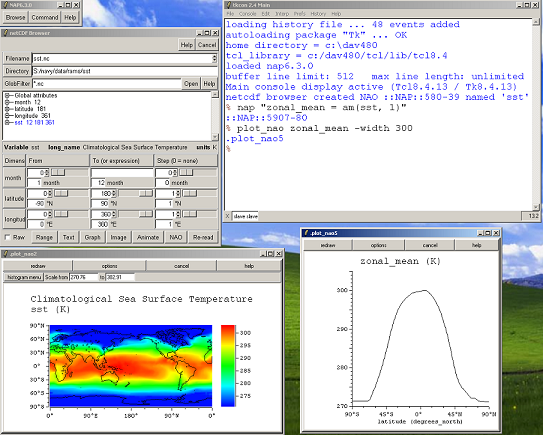
\includegraphics{screen.png}

\vspace*{15mm}

\colorbox{blue}{
    \textcolor{white}{
	\rule[-10mm]{0mm}{27mm}
	\hspace{159mm}
	\textsf{
	    {\Large www.csiro.au}
	}
	\hspace{10mm}
    }
}

\pagebreak
\mbox{}
\pagebreak
\thispagestyle{empty}
\toptitle
\pagebreak

\vspace*{140mm}
}

{
\setlength{\parindent}{0mm}
\setlength{\parskip}{0.5\baselineskip}

{\large 
Davies, Harvey, 1944- . \\
NAP {\napversion} user's guide. \\
\\	
ISBN 1 921061 18 9 (pdf.). \\
ISSN 1833-2331 \\
\\	
1. Earth Sciences - Computer programs - Handbooks, manuals, \\
etc.  2. Array processors - Handbooks, manuals, etc.  I. \\
CSIRO. Marine and Atmospheric Research.  II. Title. \\
(Series : CSIRO Marine and Atmospheric Research paper; 4). \\
\\	
\\	
550.0285
}

\pagebreak

\newcommand{\sectionlabel}[1]{
    \vspace*{6mm}
    \textbf{\textsf{\Large #1}}
    \vspace*{3mm}
}

{\large 
Enquiries should be addressed to:

Harvey L. Davies\\
CSIRO Marine and Atmospheric Research\\
Private Bag No. 1, Aspendale, Victoria 3195, Australia\\
Telephone: +61 3 9239 4556\\
Facsimile:  +61 3 9239 4444\\
Email: harvey.davies@csiro.au
}
	
\sectionlabel{Distribution list}

\begin{tabular}{|l|l|}
    \hline
    Project Manager & \hspace{15mm} \\ \hline
    On-line approval to publish & \\ \hline
    Client & \\ \hline
    Authors & \\ \hline
    Other CSIRO Staff  & \\ \hline
    National Library  & \\ \hline
    State Library & \\ \hline
    CMAR Library as pdf & \\ 
    (Meredith Hepburn) & \\ \hline
    CMAR Web Manager  as pdf & \\
    (Diana Reale) & \\ \hline
\end{tabular}

\sectionlabel{Important Notice}

\fbox{
    \begin{minipage}[t]{\textwidth}
	\setlength{\parskip}{0.5\baselineskip}
	\begin{raggedright}
	    {\sffamily
		{\copyright} Copyright Commonwealth Scientific and Industrial Research
		Organisation (`CSIRO') Australia 2006

		All rights are reserved and no part of this publication covered by copyright
		may be reproduced or copied in any form or by any means except with the written
		permission of CSIRO.

		The results and analyses contained in this Report are based on a number of
		technical, circumstantial or otherwise specified assumptions and parameters.
		The user must make its own assessment of the suitability for its use of
		the information or
		material contained in or generated from the Report. To the extent permitted by law,
		CSIRO excludes all liability to any party for expenses, losses, damages and costs
		arising directly or indirectly from using this Report.
	    }
	\end{raggedright}
    \end{minipage}
}

\sectionlabel{Use of this Report}

\begin{raggedright}
    {\sffamily
	The use of this Report is subject to the terms on which it was prepared by CSIRO.
	In particular, the Report may only be used for the following purposes.
	\begin{itemize}
	    \item
		this Report may be copied for distribution within the Client's organisation; 
	    \item
		the information in this Report may be used by the entity for which it was prepared
		(``the Client''), or by the Client's contractors and agents, for the Client's
		internal business operations (but not licensing to third parties); 
	    \item
		extracts of the Report distributed for these purposes must clearly note that the
		extract is part of a larger Report prepared by CSIRO for the Client.
	\end{itemize}
	The Report must not be used as a means of endorsement without the prior written consent
	of CSIRO.

	The name, trade mark or logo of CSIRO must not be used without the prior written
	consent of CSIRO.
    }
\end{raggedright}
}

\pagebreak
\mbox{}
\pagebreak


\tableofcontents

\chapter{Introduction}
\pagenumbering{arabic}
        % Overview of NAP
    \section{Overview of NAP (N-Dimensional Array Processor)}
\label{overview}

  \par NAP is a loadable extension of 
  \href{http://wiki.tcl.tk/}{Tcl}. NAP provides a powerful and
  efficient facility for processing data in the form of n-dimensional
  arrays. It has been designed to provide a tcl-flavoured
  array-processing facility with much of the functionality of languages
  such as 
  \href{http://www.acm.org/sigapl/}{APL}, 
  \href{http://www.fortran.com/fortran/}{Fortran-90}, 
  \href{http://www.rsinc.com/idl/index.asp}{IDL}, 
  \href{http://www.jsoftware.com/}{J}, 
  \href{http://www.mathworks.com/}{matlab} and 
  \href{http://www.octave.org/}{octave}. Three other tcl
  extensions which provide array-processing facilities are 
  \href{http://www-obs.univ-lyon1.fr/\%7Ethiebaut/TiM/TiM.html}{TiM},
  \href{http://sourceforge.net/projects/blt/}{BLT} and 
  \href{http://www.gm.com/automotive/innovations/rnd/TK3/TK3D-Software-Description.html}{ Tk3D}.
  \par Existing Tcl facilities (e.g. Tcl variables and procedures) are
  used where appropriate. The new facilities have been designed to
  match similar existing ones. In particular, NAP expressions use
  conventions which are essentially a superset of those of the Tcl 
  \texttt{expr} command. Support is provided for data based on 
  \emph{n-dimensional grids}, where the dimensions correspond to
  continuous spatial coordinates. There are interfaces to the 
  \href{http://hdf.ncsa.uiuc.edu}{HDF} and 
  \href{http://www.unidata.ucar.edu/packages/netcdf/index.html}{netCDF}
  file formats commonly used for such data, especially in Earth
  sciences such as Oceanography and Meteorology. There is a new photo
  image format for NAP data.
  \par NAP was developed as part of the CSIRO 
  \href{http://www.dar.csiro.au/rs/avhrr-processing-software.htm}{CAPS}
  project, but can be loaded and used without the (satellite oriented)
  CAPS extension. However the CAPS extension requires NAP since most
  CAPS data are stored as NAOs.
  \par Data are stored in memory as 
  \emph{n-dimensional array objects (NAOs)}, which include
  information such as:
  \begin{itemize}
    \item data-type
    \item unique ID (handle generated by NAP) called the 
    \emph{OOC-name} (OOCs are discussed below)
    \item optional label
    \item optional C format
    \item optional unit of measure
    \item reference count (allowing automatic deletion of the NAO when it
    is no longer needed)
    \item optional missing-value (used to indicate undefined data,
    etc.)
    \item rank (number of dimensions)
    \item dimension sizes
    \item optional dimension names
    \item optional pointers to 
    \emph{coordinate-variable} NAOs associated with each
    dimension
  \end{itemize}There are eleven data-types, six for integers, two for
  floating-point, one for characters, one 
  \emph{pointer} type (allowing arrays of arrays) and a 
  \emph{ragged} type providing a form of compression.
  \par NAOs are created by the Tcl commands 
  \texttt{nap} and 
  \texttt{nap\_get}.
  \par The 
  \texttt{nap} command takes arguments specifying an expression in
  a manner similar to the 
  \texttt{expr} command. However, unlike 
  \texttt{expr}, 
  \texttt{nap} provides:
  \begin{itemize}
    \item assignment (to a Tcl variable whose value is set to the
    OOC-name of the resultant NAO)
    \item substitution of Tcl names (obviating the need for `\texttt{\$}' prefixes)
    \item array facilities (constants, operators, functions,
    indexing)
  \end{itemize}Array indices can take fractional values, which are defined by
  n-dimensional linear interpolation. Index values can be specified
  indirectly via coordinate-variable values (e.g. latitudes and
  longitudes).
  \par The 
  \texttt{nap\_get} command creates a NAO from data read from a
  binary, HDF or netCDF file. Some platforms (only Linux on Intel 386
  at the time of writing) support reading of remote virtual netCDF
  files provided by 
  \href{http://www.opendap.org/}{OPeNDAP} (a.k.a. 
  \emph{DODS}) web servers.
  \par Every NAO has an associated Tcl command called an 
  \emph{object-oriented command} (
  \emph{OOC}). This is used to:
  \begin{itemize}
    \item display the data in the NAO
    \item display other information about the NAO such as its data-type
    and dimensions
    \item change data and other details
    \item write data from the NAO to a binary, HDF or netCDF file
  \end{itemize}
  \par As usual in Tcl, OOC and 
  \texttt{nap\_get} command options can be abbreviated provided
  there is no ambiguity.
  \par NAP provides many operators and built-in functions. One can define
  new functions by defining Tcl procedures with the 
  \texttt{proc} command. It is also possible to call functions
  written in C and Fortran.
  \par The 
  \emph{caps/nap GUI} provides browsers for:
  \begin{itemize}
    \item Tcl variables
    \item image files (e.g. GIF, JPEG)
    \item AVHRR satellite files (caps package required)
    \item ATSR satellite files (caps package required)
    \item CIF files (Melbourne University format)
    \item HDF/netCDF files
  \end{itemize}The HDF/netCDF browser is a convenient tool for quickly browsing
  HDF and netCDF files. Selected data can be
  \begin{itemize}
    \item displayed as text
    \item graphed
    \item shown as various kinds of images and maps
    \item animated
    \item used to create a NAO for further processing using NAP
  \end{itemize}

    %  $Id: typo.tex,v 1.3 2006/04/06 09:54:47 dav480 Exp $ 
    % Nap Typographic Conventions

\section{Typographic Conventions}

Hyperlinks are blue, as in
\href{http://tcl-nap.sourceforge.net/index.php}{tcl-nap}.
Internal references are red, as in section \ref{overview}.
Both can be clicked on if you are reading this on a screen rather than paper.
Try it.

Consider the following example:
\\
\texttt{count(}$x$[\texttt{,} $r$]\texttt{)}

The font used for `\texttt{count(,)}' indicates this is 
    \textit{literal text}. In other words this is exactly what appears
    on the screen (which could be either output or typed input). Note
    that `$x$' 
    and `$r$' are in italics (with slanted font), which
    indicates these are 
    \textit{formal argument names} rather than literal text. You
    replace such names with whatever is desired.
    
 Optional arguments are indicated using two alternative
    conventions. In the above example they are enclosed in brackets,
    indicating that `\texttt{,} $r$' is optional. This convention is common in
    computing documentation. Use has also been made of the the
    alternative (commonly used in Tcl documentation) of surrounding the
    optional component with question marks. For example:
    \\
    \texttt{count(}$x$ ?\texttt{,} $r$?\texttt{)}
    
 Alternatives are indicated with a vertical bar `\texttt{|}', as
    in the following:
    \\
    \texttt{nap\_info bytes|sequence}
    \\
    which indicates that the argument can be either `\texttt{bytes}' or `\texttt{sequence}'.

    %  $Id: ack.tex,v 1.1 2006/02/24 05:51:11 dav480 Exp $ 
    % Acknowledgments
    \section{Acknowledgments}

  Ken Iverson (who died in 2004) is the father of array
  processing. NAP does not use the radical mathematical conventions of
  his languages 
  \href{http://www.acm.org/sigapl/}{APL}, and 
  \href{http://www.jsoftware.com/}{J}, but he must be
  acknowledged as the source of the fundamental concepts upon which NAP
  is based. NAP has also adopted various J conventions such as that for
  floating-point constants (e.g. allowing 0.5 to be written in rational
  form as 
  \texttt{1r2} and allowing powers of $\pi$ as in 
  \texttt{1p1}).
  \par NAP would never have happened if the author (Harvey Davies) had
  not worked with Rhys Francis and Ian Mathieson on development of the
  data-parallel modelling language 
  \textit{DPML} and learned from them things like 
  \textit{yacc}. This project met a premature death but we did learn a
  lot. It is hoped to implement unit calculus (automatic unit
  conversion and definition) in NAP as was done in DPML.
  \par The other strong influence on NAP was 
  \href{http://www.unidata.ucar.edu/packages/netcdf/index.html}{netCDF}.
  It is amazing that a portable array file format did not exist until
  Russ Rew and the late Glenn Davis developed netCDF in the early
  1990s. This work was based on 
  \href{http://nssdc.gsfc.nasa.gov/cdf/cdf-home.html}{CDF}, which
  was developed by Michael Gough and Lloyd Treinish. NAP is designed to
  read and write netCDF (and the similar 
  \href{http://hdf.ncsa.uiuc.edu}{HDF}) files and stores data in
  memory in stuctures called 
  \textit{NAOs}, which have similar properties to netCDF variables.
  \par Peter Turner (now with CSIRO Marine Research) made significant
  contributions to the NAP code. He wrote the C code for:
  \begin{itemize}
    \item NAO photo-image handler
    \item 
    \textit{draw} and 
    \textit{fill} OOC methods
    \item morphological functions (moving\_range, dilate, erode)
  \end{itemize}He also made significant contributions to the following Tcl
  library files:
  \begin{itemize}
    \item 
      \texttt{browse\_var.tcl}
    \item 
      \texttt{caps\_nap\_menu.html}
    \item 
      \texttt{colour.tcl}
    \item 
      \texttt{hdf.tcl}
    \item 
      \texttt{pal.tcl}
    \item 
      \texttt{plot\_nao.tcl}
    \item 
      \texttt{proc\_lib.tcl}
  \end{itemize}
  \par The 
  \href{land-flag.html}{ \texttt{nap\_land\_flag} } command is based on code which was originally written by Dr.
  Chris. Mutlow at the Rutherford Appleton Laboratory in England. This
  code has been adapted for NAP by Peter Turner and Harvey Davies.
  \par Past and present members of The CAPS development group (Ian Grant,
  Edward King, Jenny Lovell, Paul Tildesley, Peter Turner and Chris
  Rathbone) have provided ideas, support and feedback over the years.
  Mark Collier and Janice Bathols were early users of NAP for
  processing results from atmospheric modelling. Their success and
  enthusiasm has has done a great deal to convert others to 
  \textit{napism}. Paul Durack produced the PDF version of the
  User's Guide.
  \par Dr Takeshi Enomoto, Earth Simulator Center, maintains the 
  \href{http://fink.sourceforge.net/pdb/package.php/nap}{nap Fink site}, which provides distributions for the 
  \textit{Mac OS X} and 
  \textit{Darwin} platforms.


\chapter{Background}
    %  $Id: tcl_log.tex,v 1.8 2006/09/20 08:48:49 dav480 Exp $ 
    % Simple Tcl/Tk

\section{Demonstration of Simple Tcl/Tk}

\subsection{Introduction}
    \label{Introduction}

The following are logs of demonstrations of simple 
  \emph{Tcl/Tk} (excluding Nap). These can be used as a starting
  point from which to explore the system.

\subsection{First Look at Tcl}
    \label{tcl1}

The following demonstrates Tcl syntax, variables and the
  following commands:
\begin{bullets}
    \item 
    \texttt{expr} (arithmetic)
    \item 
    \texttt{set} (setting and displaying variables)
    \item 
    \texttt{puts} (output)
    \item 
    \texttt{for} (looping)
\end{bullets}
  \begin{verbatim}
% expr 3.1416 * 10 * 10
314.16
% set pi 3.1416
3.1416
% set pi
3.1416
% set r 10
10
% expr $pi * $r * $r
314.16
% set area [expr $pi * $r * $r]
314.16
% puts "circle of radius $r has area $area"
circle of radius 10 has area 314.16
% puts "circle of radius $r has area [expr $pi * $r * $r]"
circle of radius 10 has area 314.16
% for {set r 4} {$r < 5.1} {set r [expr $r + 0.2]} {
puts "circle of radius $r has area [expr $pi * $r * $r]"
}
circle of radius 4 has area 50.2656
circle of radius 4.2 has area 55.417824
circle of radius 4.4 has area 60.821376
circle of radius 4.6 has area 66.476256
circle of radius 4.8 has area 72.382464
circle of radius 5.0 has area 78.54
\end{verbatim}

\subsection{First Look at Tk}
    \label{tcl-log-tk1}

Tcl was designed to be extended. One of the first extensions was
  \emph{Tk}, which provides a toolkit for building GUIs (Graphical
  User Interfaces).
  

The following demonstration is intended to provide just a hint of
  the nature of Tk. It displays two buttons which can be pressed to
  execute simple commands.
  \begin{verbatim}
% button .hello -text "press me" -command {puts "Hello world"}
.hello
% pack .hello
Hello world
% button .beep -text beep -command bell
.beep
% pack .beep
\end{verbatim}

\subsection{Syntax of Tcl}
    \label{tcl-log-syntax}

The syntax of Tcl is based on the following 
  \emph{metacharacters} (characters treated in special ways):
  \\
  \texttt{; \# \$ " $\backslash$ \{\} []}
  \\Note that the following are 
  \emph{not} metacharacters:
  \\
  \texttt{' * ()}
  \begin{verbatim}
% set s1 the; set s2 "This is $s1"; set s3 {end of it all.}
end of it all.
% puts "$s2$s3"
This is theend of it all.
% puts "${s1}2"; # Braces around name are needed when next char could be part of name
the2
% puts \
"$s2 $s3"
This is the end of it all.
% puts "$s2
$s3"
This is the
end of it all.
% puts "$s2\
$s3"
This is the end of it all.
% puts \
"$s2\n$s3"
This is the
end of it all.
% # This is a comment
% set s1; # Value of s1
the
% # Character # is only special at start:
% puts #
#
% puts [expr [string length $s2] + 1 + [string length $s3]]
26
% unset s1
% set s1
can't read "s1": no such variable
% puts [expr "2 + 2"]
4
\end{verbatim}

\subsection{Lists and Strings}
    \label{tcl-log-lists-strings}

Tcl is a 
  \emph{text-oriented} language in which text can be treated as
  either a single 
  \emph{string} or a 
  \emph{list} of elements. A sentence is a simple 
  \emph{list} of words separated by white-space. An element of a list
  can itself be a list.
  \begin{verbatim}
% set names "Bill Jan Harry"; # Simple list of 3 words
Bill Jan Harry
% lindex $names 0
Bill
% lindex $names 2
Harry
% lsort $names
Bill Harry Jan
% foreach name $names {puts "'$name' has [string length $name] letters"}
'Bill' has 4 letters
'Jan' has 3 letters
'Harry' has 5 letters
% set names {{Bill Jones} {Jan Smith} {Harry Brown}}; # list of lists
{Bill Jones} {Jan Smith} {Harry Brown}
% foreach name $names {puts "'$name' has [string length $name] letters"}
'Bill Jones' has 10 letters
'Jan Smith' has 9 letters
'Harry Brown' has 11 letters
% string toupper $names
{BILL JONES} {JAN SMITH} {HARRY BROWN}
% string map {i a rr r} $names; # change "i" to "a", "rr" to "r"
{Ball Jones} {Jan Smath} {Hary Brown}
% string index hello 0
h
% string index hello 4
o
% foreach name $names {puts "[lindex $name 1], [lindex $name 0]"}
Jones, Bill
Smith, Jan
Brown, Harry
% foreach name $names {
    foreach word $name {
       puts -nonewline [string index $word 0]
    }
    puts ""
}
BJ
JS
HB
\end{verbatim}

\subsection{File Input and Output}
    \label{tcl-log-file}

The following commands are demonstrated in the following log:
\begin{bullets}
    \item 
      \texttt{open}
    \item 
      \texttt{close}
    \item 
    \texttt{puts} (Write to file or screen)
    \item 
    \texttt{gets} (Read from file)
    \item 
    \texttt{format} (Controlled conversion of values to text)
    \item 
    \texttt{glob} (List of files matching pattern)
\end{bullets}
\begin{verbatim}
% # Write file containing height and width on each line
% set lines {{2 4} {1 1} {9 3}}
{2 4} {1 1} {9 3}
% set f [open hw.txt w]; # open file for writing
filee1c290
% foreach line $lines {puts $f $line}
% close $f
% 
% # Read this file and display: height, width, area of rectangle
% set f [open hw.txt]; # open file for reading
filee1cd80
% while {[gets $f line] >= 0} {
     set h [lindex $line 0]
     set w [lindex $line 1]
     puts "$h $w [expr $h * $w]"
}
2 4 8
1 1 1
9 3 27
% close $f
% 
% format {%s is %5.2f} {my age} 60.127
my age is 60.13
% format {%s is %8.1f} {my age} 60.127
my age is     60.1
%
% # For files *.txt: Display lines containing "if"
% foreach file [glob *.txt] {
     set f [open $file]
     while {[gets $f line] >= 0} {
         if {[string match {*if*} $line]} {puts "$file $line"}
     }
}
\end{verbatim}

\subsection{Procedures and Control Structures}
    \label{tcl-log-control}

The following shows how the 
  \texttt{proc} command can be used to define a procedure and thus
  a new command. It also illustrates the control-structure commands 
  \texttt{if}, 
  \texttt{for} and 
  \texttt{foreach}.
  \begin{verbatim}
% proc initials words {
    foreach word $words {append result [string index $word 0]}
    return $result
}
% initials {Bill Harry Jan}
BHJ
% 
% # arithmetic progression
% proc ap {
     from
     to
     {step 1}
} {
     for {set next $from} {$next <= $to} {set next [expr $next + $step]} {
         lappend result $next
     }
     return $result
}
% ap 1 9 2
1 3 5 7 9
% ap 1 9
1 2 3 4 5 6 7 8 9
% ap 0 3 0.5
0 0.5 1.0 1.5 2.0 2.5 3.0
% foreach r [ap 1 9 2] {puts "square of $r is [expr $r * $r]"}
square of 1 is 1
square of 3 is 9
square of 5 is 25
square of 7 is 49
square of 9 is 81
% 
% # Define factorial using recursion
% proc factorial n {
     if {$n > 1} {
         return [expr $n * [factorial [expr $n - 1]]]
     } else {
         return 1
     }
}
% factorial 3
6
% foreach i [ap 0 5] {puts "$i [factorial $i]"}
0 1
1 1
2 2
3 6
4 24
5 120
\end{verbatim}


    %  $Id: model.tex,v 1.7 2006/06/07 04:58:19 dav480 Exp $ 
    % NAP: Data Models

\section{Data Models}

A 
  \textit{data model} is a mental model of the nature of some data. It
  answers such questions as the following:

\subsection{What values can the data take?}

Are they all numeric? Are they
  all integers? Is the set of possible values finite? What are the
  minimum and maximum possible values? Are $\infty$ and 
  \textit{NaN} possible values? Do some values have special meanings,
  such as indicating undefined or missing data?

\subsection{What is the measurement level?}

Data is often classified as follows according to \emph{measurement level}:
\\
    \begin{tabular}{|l||p{40 mm}|p{20 mm}|p{20 mm}|p{30 mm}|}
    \hline 
      \textbf{Level} & 
      \textbf{Description} & 
      \textbf{Valid \mbox{Operations}} & 
      \textbf{Measure of Central\ Tendency} & 
      \textbf{Examples}
    \\
    \hline 
    \hline 
      nominal & 
      Values denote categories which have no order & 
      = $\neq$ & 
      mode & 
      \mbox{zip post-code} \mbox{chemical e.g. CO$_{2}$}
    \\
    \hline 
      ordinal & 
      \mbox{Values ordered} \mbox{Differences meaningless} & 
      = $\neq$ $<$ $\le$ $>$ $\ge$ & 
      median & 
      Richter earthquake scale
    \\
    \hline 
      interval & 
      \mbox{Differences valid} \mbox{Quotients meaningless} & 
      $= \neq < \le > \ge + -$ & 
      arithmetic mean & 
      temperature in $^{\circ}$C
    \\
    \hline 
      ratio & 
      Quotients valid & 
      $= \neq < \le > \ge + - \times \div $ & 
      geometric mean & 
      temperature in $^{\circ}$K 
    \\
  \hline
\end{tabular}

\subsection{How accurate are the values?}

A \textit{measurement error} is the difference between the 
  \textit{true value} and the 
  \textit{measured value}. Measured values can differ from true values
  due to:
\begin{bullets}
    \item finite precision of instrument
    \item systematic errors (e.g. inadequately calibrated
    instrument)
    \item random errors (due to finite size of sample)
    \item sampling errors (due to non-randomness of sample)
    \item blunders (e.g. a human misreading an instrument)
\end{bullets}
It is desirable to include error estimates with data.

\subsection{Are the data located in some space?}

A \textit{time series} consists of values located along the time
  dimension. 
  \textit{Geographic} data is located along spatial dimensions such as
  latitude, longitude and altitude and may also have a time dimension.
  Note that longitude is 
  \textit{cyclic}.

The dimensions of the space can have a measurement level of \textit{nominal}.
For example, an accounting spreadsheet might have columns corresponding to 
\textit{charge codes} and rows corresponding to \textit{company divisions}.

Some variables have a vector value at each point in space and time.
For example, wind data is typically stored as two (east and north) components. 
These components are often treated as separate variables.
An alternative approach is to have a single array whose dimensions include a
\textit{nominal} dimension corresponding to the components.
Thus a wind array could include a dimension of size 2 corresponding to east and north.

Data located in a continuous space can be either 
  \textit{gridded} or 
  \textit{scattered}. Both types are discussed in section \ref{grid} (Nap Grids).

    %  $Id: term.tex,v 1.6 2006/09/20 08:48:49 dav480 Exp $ 
    % Nap Terminology

\section{Terminology}

\subsection{Arrays}

    \begin{description}
      \item[scalar]
      array with 0 dimensions i.e. a simple number, character,
      etc.
      \item[vector]
      array with 1 dimension.
      \item[matrix]
      array with 2 dimensions.
      \item[dimension-size]
      number of values along a dimension.
      \item[shape]
      vector of dimension-sizes of array.
      \item[rank]
      number of dimensions (a.k.a. dimensionality) i.e. shape of
      shape.
      \item[column]
      final (least-significant) dimension
      \item[dimension-name]
      name given to dimension e.g. "latitude".
      \item[coordinate-variable (CV)]
      vector (usually sorted) associated with a dimension of the
      same size. CVs are often used to map an array's dimensions to
      physical dimensions such as length and time, thus locating the
      array elements in physical space and time.
    \end{description}

\subsection{Special Numeric Values}

    \begin{description}
      \item[missing-value (MV)]
      numeric value of data which is abnormal in some way such as:
\begin{bullets}
	    \item not applicable (e.g. land point for ocean data)
	    \item not available (e.g. instrument failure or delay in obtaining data)
	    \item result of some illegal operation such as dividing 0 by 0
	    \item undefined for some other reason 
\end{bullets}
      \item[infinity ($\infty$)]
      floating-point value representing a value which is too
          large (or small in the case of $-\infty$) to
          represent. This can result from operations such as dividing
          by 0.
      \item[NaN (not-a-number)]
      floating-point value resulting from an illegal operation
          such as dividing 0 by 0.
    \end{description}

    %  $Id: grid.tex,v 1.6 2006/05/04 04:49:04 dav480 Exp $ 
    % Nap Grids

\section{Grids}
    \label{grid}

\subsection{Dimensions, Coordinate variables and Mappings}
    \label{grid-Dims}

Traditional array-processors, such as APL, are based on a
  data-model which has discrete dimensions whose corresponding
  subscripts take integer values. Nap handles such traditional arrays
  in the traditional manner. However Nap is based on a more general
  data-model which also allows non-integer subscript values. These
  values represent distances along dimensions which often correspond to
  the physical dimensions of spacio-temporal spaces, which are of
  course continuous.

If desired, a dimension can have an associated variable called the
  \textit{coordinate variable (CV)}. This is a vector which defines a
  piecewise-linear mapping from subscript to physical dimension.

\emph{Nominal} dimensions often have text labels associated with each value.
For example, wind components could be labelled `\texttt{east}' and `\texttt{north}'.
One could imagine some kind of CV containing such string values.
Nap does allow a string CV, but there can be only a single character for each value.
So in the wind case one would have to make do with a string CV with a value such as `\texttt{EN}'.

CVs are convenient when each array dimension maps to a single
  physical dimension. However, the relationship between array
  dimensions and physical dimensions may be more complex. Consider the
  example of a satellite image with dimensions 
  \textit{line} (row) and 
  \textit{pixel} (column). The physical dimension 
  \textit{latitude} depends on both array dimensions (\textit{line} and 
  \textit{pixel}). There is a matrix (with the same 
  \textit{line} and 
  \textit{pixel} dimensions as the image) giving the latitude at each
  point. There is another similar longitude matrix. These two matrices
  define piecewise-bilinear mappings from line/pixel space to
  latitude/longitude space. The task of warping the image to
  latitude/longitude space is essentially that of defining mappings
  from latitude/longitude space to line/pixel space i.e. the inverses
  of the given mappings. This can be done using the Nap functions 
{\texttt{invert\_grid} and \texttt{invert\_grid\_no\_trim}},
which are discussed in section \ref{function-Grid}.

\subsection{Difference between Grids and Scattered Data}
    \label{grid-Dif}

Data in a continuous space with two or more dimensions can be
  either 
  \textit{gridded} or 
  \textit{scattered}. Nap's data-model (with continuous subscripts,
  coordinate variables, etc.) facilitates the processing of gridded
  data.

Let us consider the case of two dimensions i.e. matrices.
  Two-dimensional 
  \textit{gridded} data is aligned in rows and columns, whereas 
  \textit{scattered} data is not. The following examples are intended
  to illustrate the difference between 
  \textit{scattered} and 
  \textit{gridded} 2D data.

\subsubsection{Example of Scattered 2D Data (Not a Grid)}

Note that the data are not aligned in rows and columns.

  \begin{tabular}{|*{9}{p{6 mm}}|}
      \hline 
       & 
       & 
       & 
      $\bullet$
       & 
       & 
       & 
       & 
       & 
    \\
      $\bullet$
       & 
       & 
       & 
       & 
       & 
      $\bullet$
       & 
       & 
       & 
    \\
       & 
       & 
       & 
       & 
       & 
       & 
       & 
       & 
    \\
       & 
       & 
       & 
       & 
      $\bullet$ 
       & 
       & 
       & 
       & 
    \\
       & 
       & 
       & 
       & 
       & 
      $\bullet$
       & 
       & 
       & 
    \\
       & 
       & 
       & 
       & 
       & 
       & 
       & 
      $\bullet$
       & 
    \\
       & 
       & 
       & 
       & 
       & 
       & 
       & 
       & 
    \\
       & 
       & 
       & 
       & 
       & 
       & 
       & 
       & 
    \\
       & 
       & 
       & 
       & 
       & 
       & 
       & 
       & 
    \\
       & 
      $\bullet$
       & 
       & 
       & 
       & 
       & 
       & 
       & 
    \\
       & 
       & 
       & 
       & 
       & 
       & 
       & 
       & 
      $\bullet$
    \\
       & 
       & 
       & 
       & 
       & 
       & 
       & 
       & 
    \\
       & 
       & 
       & 
       & 
       & 
       & 
       & 
       & 
    \\
       & 
       & 
       & 
       & 
       & 
       & 
      $\bullet$
       & 
       & 
    \\
      \hline 
\end{tabular}

\subsubsection{Example of 2D Grid}
    \label{grid-ex2dgrid}

The following example has the grid in black. The green point is not
  on the grid and has non-integer subscript values (2.1, 1.6). The
  coordinate variables are latitude and longitude.

    \begin{tabular}{|lrl|cccccc|}
      \hline 
         & 
         & 
        column & 
        0 & 
        1 & 
	\textcolor{green}{1.6}
         & 
        2 & 
        3 & 
        4
      \\
         & 
         & 
        longitude & 
        30$^{\circ}$E & 
        40$^{\circ}$E & 
	\textcolor{green}{52$^{\circ}$E}
         & 
        60$^{\circ}$E & 
        65$^{\circ}$E & 
        75$^{\circ}$E
      \\
        row & 
        latitude
         & 
         & 
         & 
         & 
         & 
         & 
         & 
      \\
      \hline 
        0 & 
        30$^{\circ}$N & 
         & 
        $\bullet$ & 
        $\bullet$ & 
         & 
        $\bullet$ & 
        $\bullet$ & 
        $\bullet$
      \\
        1 & 
        25$^{\circ}$N & 
         & 
        $\bullet$ & 
        $\bullet$ & 
         & 
        $\bullet$ & 
        $\bullet$ & 
        $\bullet$ 
      \\
        2 & 
        10$^{\circ}$N & 
         & 
        $\bullet$ & 
        $\bullet$ & 
         & 
        $\bullet$ & 
        $\bullet$ & 
        $\bullet$ 
      \\
	\textcolor{green}{2.1}
         & 
	\textcolor{green}{8$^{\circ}$N}
         & 
         & 
         & 
         & 
\textcolor{green}{$\bullet$}
         & 
         & 
         & 
      \\
        3 & 
        10$^{\circ}$S & 
         & 
        $\bullet$ & 
        $\bullet$ & 
         & 
        $\bullet$ & 
        $\bullet$ & 
        $\bullet$
      \\
      \hline 
\end{tabular}

\subsection{Missing Data}
    \label{grid-Missing}

The Nap data model allows any element of an array to have a
  value which is a 
  \textit{missing-value}. Such elements are considered null or missing
  and are treated specially in operations such as arithmetic. Thus
  adding a missing value to anything produces a missing value.

The following example is similar to that above. However four grid
  points are missing. These are shown in red.

    \begin{tabular}{|lrl|cccccc|}
      \hline 
         & 
         & 
        column & 
        0 & 
        1 & 
	\textcolor{green}{1.6}
         & 
        2 & 
        3 & 
        4
      \\
         & 
         & 
        longitude & 
        30$^{\circ}$E & 
        40$^{\circ}$E & 
	\textcolor{green}{52$^{\circ}$E}
         & 
        60$^{\circ}$E & 
        65$^{\circ}$E & 
        75$^{\circ}$E
      \\
        row & 
        latitude
         & 
         & 
         & 
         & 
         & 
         & 
         & 
      \\
      \hline 
        0 & 
        30$^{\circ}$N & 
         & 
        $\bullet$ & 
        $\bullet$ & 
         & 
        $\bullet$ & 
	\textcolor{red}{$\bullet$} & 
        $\bullet$
      \\
        1 & 
        25$^{\circ}$N & 
         & 
        $\bullet$ & 
        $\bullet$ & 
         & 
        $\bullet$ & 
        $\bullet$ & 
        $\bullet$ 
      \\
        2 & 
        10$^{\circ}$N & 
         & 
	\textcolor{red}{$\bullet$}
         & 
        $\bullet$ & 
         & 
        $\bullet$ & 
        $\bullet$ & 
	\textcolor{red}{$\bullet$}
      \\
	\textcolor{green}{2.1}
         & 
	\textcolor{green}{8$^{\circ}$N}
         & 
         & 
         & 
         & 
\textcolor{green}{$\bullet$}
         & 
         & 
         & 
      \\
        3 & 
        10$^{\circ}$S & 
         & 
        $\bullet$ & 
        $\bullet$ & 
         & 
	\textcolor{red}{$\bullet$}
         & 
        $\bullet$ & 
        $\bullet$
      \\
      \hline 
\end{tabular}

  The missing points are treated as if they did not exist, as shown
  in the following:

    \begin{tabular}{|lrl|cccccc|}
      \hline 
         & 
         & 
        column & 
        0 & 
        1 & 
	\textcolor{green}{1.6}
         & 
        2 & 
        3 & 
        4
      \\
         & 
         & 
        longitude & 
        30$^{\circ}$E & 
        40$^{\circ}$E & 
	\textcolor{green}{52$^{\circ}$E}
         & 
        60$^{\circ}$E & 
        65$^{\circ}$E & 
        75$^{\circ}$E
      \\
        row & 
        latitude
         & 
         & 
         & 
         & 
         & 
         & 
         & 
      \\
      \hline 
        0 & 
        30$^{\circ}$N & 
         & 
        $\bullet$ & 
        $\bullet$ & 
         & 
        $\bullet$ & 
	& 
        $\bullet$
      \\
        1 & 
        25$^{\circ}$N & 
         & 
        $\bullet$ & 
        $\bullet$ & 
         & 
        $\bullet$ & 
        $\bullet$ & 
        $\bullet$ 
      \\
        2 & 
        10$^{\circ}$N & 
         & 
         & 
        $\bullet$ & 
         & 
        $\bullet$ & 
        $\bullet$ & 
      \\
	\textcolor{green}{2.1}
         & 
	\textcolor{green}{8$^{\circ}$N}
         & 
         & 
         & 
         & 
\textcolor{green}{$\bullet$}
         & 
         & 
         & 
      \\
        3 & 
        10$^{\circ}$S & 
         & 
        $\bullet$ & 
        $\bullet$ & 
         & 
         & 
        $\bullet$ & 
        $\bullet$
      \\
      \hline 
\end{tabular}

It would be possible to represent scattered data by a grid with
  many missing points. In the extreme, each scattered point would have
  its own row and its own column. There would be only one non-missing
  point in each row. There would be only one non-missing point in each
  column. Of course this would be very inefficient for a matrix of
  significant size.

\subsection{Processing Scattered Data}
    \label{grid-Scattered}

Function 
{\texttt{scattered2grid} } interpolates scattered data onto a grid.
See section
  \ref{nap-function-lib-scattered2grid}
for details.

    %  $Id: hdf_netcdf.tex,v 1.2 2007/01/01 23:31:26 dav480 Exp $ 

\section{HDF and netCDF File Formats} 
    \label{hdf-netcdf}

  \href{http://www.hdfgroup.org/}{HDF} and 
  \href{http://www.unidata.ucar.edu/packages/netcdf/index.html}{netCDF}
  are similar array-oriented file formats.
Such files are popular in earth sciences such as meteorology and oceanography.
They contain data referenced by
symbol tables containing the names, data-types and dimensions of entities called
\emph{variables} in netCDF and \emph{scientific data sets (SDSs)} in HDF.
Each variable (SDS) can also have attributes such as a label, a
  format, a unit of measure and a missing-value. 

The design of Nap has been strongly influenced by HDF and netCDF.
Nap stores data in memory structures called \emph{n-dimensional array objects} (\emph{NAOs})
that have similar attributes to those of HDF SDSs and netCDF variables
(e.g. label, format, unit of measure, missing-value). 
Nap has powerful high-level facilities for HDF and netCDF I/O.

Nap does not currently support the new 
\href{http://www.hdfgroup.org/whatishdf5.html}{HDF5}
file format.
Note that
\href{http://www.unidata.ucar.edu/software/netcdf/netcdf-4/}{netCDF-4} software
supports this HDF5 file format (as well as the traditional netCDF format)
and is due for official release in late 2006.
It is planned to support HDF5 and netCDF-4 in a future version of Nap.

    %  $Id: refs.tex,v 1.1 2006/02/28 00:09:32 dav480 Exp $ 
    % References
    \section{References}

  \subsection{
    \label{Introduction}Introduction
  }
The following provides a guide to books, papers and web sites
  relevant to NAP. The opinions are those of the author (Harvey
  Davies).
  \subsection{
    \label{tcl}Tcl/Tk
  }
The following are my three favourite Tcl/Tk web sites:
  \begin{description}
    \item[
      \href{http://wiki.tcl.tk}{wiki.tcl.tk}
    ]
    Wiki-based open community site. Excellent starting point.
    \item[
      \href{http://www.tcl.tk}{www.tcl.tk}
    ]
    Main Tcl Developer Xchange site.
    \item[
      \href{http://www.activestate.com/Products/ActiveTcl/}{www.activestate.com/Products/ActiveTcl/}
    ]
    ActiveState provide ActiveTcl here for downloading.
  \end{description}
  \par Despite its age, I consider John Ousterhout's 1994 
  \emph{Tcl and the Tk Toolkit} to still be the best introduction
  to Tcl/Tk. In fact it really is a classic example of clear readable
  technical writing. Ousterhout was the original developer of Tcl. Tcl
  has developed a lot since 1994 and the new features missing from this
  book are discussed in the 
  \href{http://wiki.tcl.tk/103}{Wiki}.
  \par The only detailed up-to-date book is the much less readable 4th
  edition of 
  \emph{Practical Programming in Tcl and Tk} by Brent Welch and
  Ken Jones with Jeffrey Hobbs. This book has the web site 
  \href{http://www.beedub.com/book}{www.beedub.com/book}.
  \subsection{
    \label{NAP}NAP
  }
The home page for 
  \emph{nap} (a.k.a.
  \emph{tcl-nap}) is at 
  \href{http://tcl-nap.sourceforge.net/index.php}{http://tcl-nap.sourceforge.net/index.php}.
The main documentation of NAP is provided by the
  \href{http://tcl-nap.sourceforge.net/nap_users_guide.pdf}{NAP User's Guide},
which is what you are reading.
  \par The only published paper on NAP is Harvey Davies's talk 
  \emph{The NAP (N-Dimensional Array Processor) Extension to Tcl}
  , which was given at the 9th (2002) Annual Tcl/Tk Conference.
Both the
\href{http://aspn.activestate.com/ASPN/Tcl/TclConferencePapers2002/Tcl2002papers/davies-nap/nap.pdf}{original}
and a
  \href{http://tcl-nap.sourceforge.net/nap_paper2002.pdf}{revised} version are available.
  \par NAP was originally developed as part of the CSIRO CAPS project,
  which has the web page 
  \href{http://www.eoc.csiro.au/cats/caps/}{http://www.eoc.csiro.au/cats/caps/}.

  \subsection{
    \label{array}Array Processing
  }
There are two main array processing professional associations in
  the world. The USA has the ACM 
  \emph{Special Interest Group on the APL and J languages}, which has
  the web page 
  \href{http://www.acm.org/sigapl}{www.acm.org/sigapl}. The
  British Computer Society has a specialist group the 
  \emph{British APL Association}, which publishes the journal 
  \emph{Vector}, which has the web page 
  \href{http://www.vector.org.uk}{www.vector.org.uk}. Both
  associations were originally concerned with only APL but now include
  other array processing languages.
  \par The primary site for the J language is 
  \href{http://www.jsoftware.com}{www.jsoftware.com}.
  \subsection{
    \label{file}Array-oriented File Formats
  }
The primary site for netCDF is 
  \href{http://www.unidata.ucar.edu/packages/netcdf/index.html}{www.unidata.ucar.edu/packages/netcdf/index.html}.
  \\The primary site for HDF is 
  \href{http://hdf.ncsa.uiuc.edu}{hdf.ncsa.uiuc.edu}.
  \subsection{
    \label{Arithmetic}Arithmetic
  }
The classic article on floating-point arithmetic (and the IEEE
  Standard 754 for it) is David Goldberg's 
  \href{http://delivery.acm.org/10.1145/110000/103163/p5-goldberg.pdf?key1=103163$\backslash$\&amp;key2=9533216011$\backslash$\&amp;coll=GUIDE$\backslash$\&amp;dl=ACM$\backslash$\&amp;CFID=36776917$\backslash$\&amp;CFTOKEN=647870}{ \emph{What Every Computer Scientist Should Know About Floating-Point Arithmetic} }, ACM Computing Surveys, 1991. A more recent paper is Kahan's
  \href{http://www.cs.berkeley.edu/~wkahan/ieee754status/ieee754.ps} {\emph{Lecture 
    Notes on the Status of IEEE 754} }.


\chapter{Installation}
    %  $Id: install.tex,v 1.9 2006/09/20 08:48:49 dav480 Exp $ 
    % Installing Tcl/Tk and NAP

\section{Installing Tcl/Tk and Nap}

\subsection{Introduction}
    \label{install-Introduction}

  \emph{Tcl/Tk} and 
  \emph{Nap} are available without charge in both binary (compiled)
  and source-code form. The following instructions explain how to
  install Tcl/Tk and then Nap. The Nap installer for Linux on the
  (64-bit) Intel IA64 installs the total system since this platform is
  not supported by ActiveState.

\subsection{Installing Tcl/Tk}
    \label{install-Installing-Tcl-Tk}

  \href{http://aspn.activestate.com/ASPN//}{ActiveState Corporation} provides free binary distributions of 
  \emph{Tcl/Tk} with many extensions. There are versions for Windows,
  Linux (on Intel 386), SunOS (Solaris) and HP-UX. HTML documentation
  is also available. These can all be downloaded from 
  \href{http://aspn.activestate.com/ASPN/Tcl/Downloads/}{ActiveState Tcl Downloads}.
  
 Read the 
  \href{http://aspn.activestate.com/ASPN/docs/ActiveTcl/at.install.html}{ installation instructions}. Note that these explain how to
  uninstall any existing version of Tcl/Tk, which should be done before
  installing the new one. (If this method of uninstalling fails then it
  is usually best to delete the whole 
  \emph{tcl root directory}.)
  
 The 
  \emph{tcl root directory} is the directory in which Tcl is
  installed. Tcl extensions (e.g. Nap) are usually also installed in
  it. Note that it is denoted below by the variable 
  $tcl\_root$. A typical value for Windows is 
  \texttt{C:$\backslash$Program\ Files$\backslash$Tcl}. Typical values for Unix
  (including Linux) are 
  \verb!~/tcl! (personal installation) and 
  \verb!/usr/local/tcl! (system installation).
  
 Unix users should include 
  $tcl\_root$\texttt{/bin} in the list defined by the standard environment
  variable 
  \texttt{PATH}. If there are problems with dynamic loading then
  try including 
  $tcl\_root$\texttt{/lib} in the list defined by the standard environment
  variable 
  \texttt{LD\_LIBRARY\_PATH}.
  
 The following three executables will be installed in 
  $tcl\_root$\texttt{/bin}:
  \begin{description}
    \item[\texttt{tclsh}]
    This provides a bare-bones command-line 
    \emph{Tcl shell} without Tk. (Tk provides GUI facilities.) It is
    useful for non-interactive applications such as 
\begin{bullets}
    \item Unix shell scripts using Tcl
    \item automatically run (e.g.  \texttt{cron}) jobs using Tcl
\end{bullets}
    \item[\texttt{wish}]
    This 
    \emph{window shell} provides a full Tcl shell including Tk.
    \item[\texttt{tkcon}]
    This provides all the facilities of 
    \texttt{wish}, but in a better console. It is recommended as
    the normal way of running Tcl.
  \end{description}
  
 Each executable will execute a startup script file with the name
  listed in the following table, if this file is found in the home
  directory:

\begin{tabular}{|l||l|l|l|}
    \hline 
      \textbf{Operating System} & 
      \textbf{tclsh} & 
      \textbf{wish} & 
      \textbf{tkcon}
    \\
    \hline 
    \hline 
        \textbf{Windows}
       & 
        \texttt{tclshrc.tcl}
       & 
        \texttt{wishrc.tcl}
       & 
        \texttt{tkcon.cfg}
    \\
    \hline 
        \textbf{Unix}
       & 
        \texttt{.tclshrc}
       & 
        \texttt{.wishrc}
       & 
        \texttt{.tkconrc}
    \\
  \hline
\end{tabular}
  
 If you are unsure of which directory is 
  \emph{home}, then enter the following two commands: 
  \texttt{
  \\cd
  \\pwd}

\subsection{Tcl/Tk Documentation}
    \label{install-tcl-doc}

The Caps/Nap Menu
  \emph{help} menu includes the remote web 
  \href{http://aspn.activestate.com/ASPN/Tcl/Reference/}{Tcl Documentation}.

  The above installation process for Windows installs this
  documentation in the form of the compiled HTML help file 
  \texttt{ActiveTclHelp.chm}. Under Windows, the above help menu
  does include this local copy of the documentation.
  
 The standard installation for Unix installs 
  \texttt{man} pages in the directory 
  $tcl\_root$\texttt{/man}. If you want to use these then include this
  directory in 
  \texttt{MANPATH}.
  
 It is also possible to create a local copy of this documentation
  in HTML form.
Under Unix, this allows the Caps/Nap Menu
  (see section \ref{caps-nap-menu})
 to provide a local
  copy of the Tcl Documentation (similar to that for Windows). To do
  this, download the the HTML documentation into the directory 
  $tcl\_root$\texttt{/doc}. Then unpack the tar file and create a symbolic
  link 
  $tcl\_root$\texttt{/doc/html} pointing to the root directory of the unpacked
  files.
  
 For example, if the Tcl root directory is 
  \verb!~/tcl! then download the version 8.4.9 file 
  \\
  \texttt{ActiveTcl8.4.9.0.121397-html.tar.gz} into the directory 
  \verb!~/tcl/doc/!.
  \\
Change to this directory and then unpack the file using a command such as
  \\
  \texttt{gtar zxf ActiveTcl8.4.9.0.121397-html.tar.gz}
  \\or
  \\
  \texttt{gunzip $<$ gtar zxf ActiveTcl8.4.9.0.121397-html.tar.gz | tar xf -}
  \\Then create the symbolic link using
  \\
  \texttt{ln -s ActiveTcl8.4.9.0.121397-html html}

\subsection{Installing Nap}
    \label{install-Installing-nap}

  \emph{Nap installers} are available for:
\begin{bullets}
    \item Linux on Intel 386
    \item Linux on IA64
    \item SunOS
    \item Windows
\end{bullets}
  
 The 
  \emph{Mac OS X} and 
  \emph{Darwin} platforms are supported via the 
  \href{http://fink.sourceforge.net}{Fink} project, which has a 
  \href{http://fink.sourceforge.net/pdb/package.php/nap}{nap}
  page.
  
 It is hoped to support HP-UX in the near future. The SGI Irix
  platform is no longer supported.
  
 Note that the Linux IA64 installer installs a total tcl system as
  well as Nap. This platform does not have an uninstaller, so it is
  suggested you install into a completely new directory rather than
  over an existing installation. 
For example, if your installation directory is 
\verb!~/tcl! you could do the following:
  \begin{verbatim}
mv ~/tcl ~/tcl_old
mkdir ~/tcl
\end{verbatim}
  
 The above installers can be downloaded from the page selected by clicking
 `Files for Downloading'  on
  \href{http://tcl-nap.sourceforge.net/}
  {http://tcl-nap.sourceforge.net/}.
They are in the form of 
  \emph{starpacks}, which are self-contained binary executables which
  contain the files to be installed. Starpacks are themselves based on
  Tcl and are described in 
  \href{http://www.equi4.com/papers/skpaper1.html}{ \emph{Beyond TclKit - Starkits, Starpacks and other *stuff} }.
  
 Then you simply execute the installer. It will first prompt you
  for the directory in which to install Nap, which is usually the 
  \emph{Tcl root directory}. Then it will check for existing Nap
  files and offer to delete them (strongly recommended) if any are
  found.
  
 Finally it will offer to install three 
  \emph{standard Nap startup script files} (with the names in the
  above table) in your home directory. It is recommended that you
  install these unless you have alternative startup files. Such
  alternative files can include the following commands to facilitate
  use of Nap: 
  \texttt{
  \\package require nap
  \\namespace import ::NAP::*}
  \\If there will be other users then copy the three startup files
  to their home directories.
  
 The script files 
  \verb!~/my_tkcon.cfg! and 
  \verb!~/my.tcl! will be sourced if they exist. You can create 
  \verb!~/my_tkcon.cfg! to tailor the tkcon console to your
  personal requirements. You can create 
  \verb!~/my.tcl! to tailor other aspects of the Tcl system to
  your personal requirements. See section
  \ref{scripts-Sample-Startup-Scripts}
for examples.
  
 These scripts and the standard Nap startup scripts are
  interrelated. The script 
  \texttt{tkcon.cfg} (\texttt{.tkconrc}) sources 
  \verb!~/my_tkcon.cfg! and initialises tkcon to source 
  \texttt{wishrc.tcl} (\texttt{.wishrc}). The script 
  \texttt{wishrc.tcl} (\texttt{.wishrc}) in turn sources 
  \texttt{tclshrc.tcl} (\texttt{.tclshrc}), which sources 
  \verb!~/my.tcl!.
  
 On Unix systems it is possible to install Nap in a directory
  (which we will denote by 
  $nap\_root$) other than the 
  \emph{Tcl root directory}. If 
  $nap\_root$\ $\neq$\  
  $tcl\_root$ then 
  $nap\_root$\texttt{/lib} must be included in the lists defined by:
\begin{bullets}
    \item the standard Tcl variable 
    \texttt{auto\_path}
    \item the standard environment variable 
    \texttt{LD\_LIBRARY\_PATH}.
\end{bullets}
For example, assume Nap is installed in 
  \verb!~/alt!. 
The following two commands are included in 
  \texttt{tclshrc.tcl} or 
  \texttt{.tclshrc}:
\begin{verbatim}
lappend auto_path ~/alt/lib
set env(LD_LIBRARY_PATH) ":~/alt/lib:$env(LD_LIBRARY_PATH)"
\end{verbatim}

\subsection{Nap User's Guide}
    \label{install-nap-doc}

The above installation process installs a copy of the Nap User's Guide
as file
\\
$nap\_root$\texttt{/lib/nap?.?/nap\_users\_guide.pdf}
(where \texttt{?.?} is the version number).
The Caps/Nap Menu (see section \ref{caps-nap-menu})
\emph{help} menu includes this local copy as well as the remote web copy at
\href{http://tcl-nap.sourceforge.net/nap\_users\_guide.pdf}
{http://tcl-nap.sourceforge.net/nap\_users\_guide.pdf}.

\subsection{Nap Source Code}
    \label{install-source}

Source code for Nap is maintained using CVS and can be accessed
  by:
\begin{bullets}
    \item 
      \href{http://tcl-nap.cvs.sourceforge.net/tcl-nap/}{Browsing CVS Source Repository}
    \item 
      \href{http://sourceforge.net/cvs/?group_id=55616}{Using
	a CVS client to access CVS Source Repository}
    \item Downloading tar file from 
    \href{http://sourceforge.net/project/showfiles.php?group_id=55616}{Tcl-Nap Files}.
\end{bullets}

\subsection{Related Packages}
    \label{install-Related-Packages}

Nap now provides the functionality previously provided by the
  (now obsolete) separate packages 
  \emph{convert\_date}, 
  \emph{inform} and 
  \emph{land\_flag}. 
However 
\href{http://www.eoc.csiro.au/cats/caps/}{Caps}
is still separate.
  
 The Windows Nap distribution now includes the 
  \href{http://lbayuk.home.mindspring.com/ezprint/}{ \emph{ezprint} }
	utility, which provides access to printers. No such separate
  printing package is needed for Unix. Previous versions of Nap used
  the 
  \emph{printer} package to provide access to printers on all
  platforms.
  
 Previous versions of Nap provided an interface to the vector
  facility in the package 
  \href{http://sourceforge.net/projects/blt/}{BLT}. This allowed
  use of the BLT 
  \emph{graph} command, which was used at that time by the Nap
  procedure 
  \emph{plot\_nao}. Nap no longer provides an interface to BLT or uses
  it in any way.

    %  $Id: scripts.tex,v 1.6 2006/06/07 04:58:22 dav480 Exp $ 
    % Sample Startup Scripts

\section{Sample Startup Scripts}
    \label{scripts}
    \label{scripts-Sample-Startup-Scripts}

\subsection{Introduction}
    \label{scripts-Introduction}

These startup scripts tailor 
  \emph{Tcl} and 
  \emph{tkcon} to personal requirements. The scripts can be copied to
  your home directory and modified as desired.

\subsection{Script \texttt{my.tcl}}
    \label{scripts-my}

The script 
  \verb!~/my.tcl! is called by the script 
  \verb!~/.tclshrc! or 
  \verb!~/tclshrc.tcl! that is created by the standard nap
  installation. This 
  \verb!~/my.tcl! script can be used to tailor Tcl in various
  ways such as
\begin{bullets}
    \item initialising packages
    \item initialising libraries
    \item defining procedures
    \item sourcing other scripts
\end{bullets}
  
 The following sample script initialises a personal library and
  defines some simple aliases:
  \begin{verbatim}
# my.tcl --
#
# Initialise my library of Tcl procedures (including Nap functions) by
sourcing its tclIndex.
# The library consists of files in directory ~/my_tcl_lib
# The file tclIndex is created by the following command:
#     auto_mkindex ~/my_tcl_lib *.tcl
foreach dir {~/my_tcl_lib} {source $dir/tclIndex}
#
proc define_alias {alias args} {proc $alias args "eval $args \$args"}
#
define_alias e expr
define_alias n nap
define_alias p pwd
define_alias cp file copy
define_alias md file mkdir
define_alias rm file delete
\end{verbatim}

\subsection{Script \texttt{my\_tkcon.tcl}}
    \label{scripts-my-tkcon}

The script 
  \verb!~/my_tkcon.tcl! is called by the script 
  \verb!~/.tkconrc! or 
  \verb!~/tkcon.cfg! that is created by the standard nap
  installation. This 
  \verb!~/my_tkcon.tcl! script can be used to tailor various
  aspects of tkcon.
  
 The following sample script defines
\begin{bullets}
    \item the font used by tkcon
    \item the number of rows and columns provided by tkcon
    \item the number of commands in history
    \item the prompt at start of each input line
\end{bullets}
\begin{verbatim}
# my_tkcon.cfg --
#
set ::tkcon::OPT(font) "Courier 10"
set ::tkcon::OPT(rows) 40
set ::tkcon::OPT(cols) 80
set ::tkcon::OPT(history) 200; # number of commands in history
set ::tkcon::OPT(prompt1) {% };# prompt at start of each input line
# set ::tkcon::OPT(prompt1) {[history nextid] % };# alternative
\end{verbatim}



\chapter{Nap Basics}
    %  $Id: sample.tex,v 1.9 2006/09/20 08:48:49 dav480 Exp $ 
    % Nap Sample Session

\section{Sample Session}

The following sample session illustrates some basic features of
    Nap. The input command lines begin with the standard Tcl prompt
    `\texttt{\%}'.
    \begin{verbatim}
% nap "x = {2 2.5 5}"
::NAP::13-13
% nap "y = x * x"
::NAP::14-14
% $y
4 6.25 25
\end{verbatim}

The first command assigns to 
    \texttt{x} a vector containing the three elements 2, 2.5 and 5.
    The second command assigns to 
    \texttt{y} a vector containing the three elements which are the
    squares of the corresponding elements of 
    \texttt{x}. The command `\texttt{\$y}' displays the value of 
    \texttt{y}.

Nap stores each variable in memory using a data-structure called
    an 
    \emph{n-dimensional array object} (\emph{NAO}).
    Each NAO has an associated Tcl command called its 
    \emph{object-oriented command} (\emph{OOC}) which is used to
\begin{bullets}
      \item obtain data and other information from the NAO
      \item write data from the NAO to files
      \item modify the NAO.
\end{bullets}
An \emph{OOC-name} (command-name of an OOC) is used
\begin{bullets}
      \item to execute the OOC (like any other Tcl command)
      \item as a unique identifier for the NAO associated with the OOC.
\end{bullets}
An OOC-name has the form 
      `\texttt{::NAP::}\emph{seq}\texttt{-}\emph{slot}', where
\begin{simpleitems}
      \item 
      \texttt{::NAP::} is the Tcl namespace used by NAP
      \item 
      \emph{seq} is the \emph{sequence number} assigned in order of creation
      \item 
      \emph{slot} is the index of an internal table used to provide fast access.
\end{simpleitems}
In the above example, both OOC-names (\texttt{::NAP::13-13} and 
      \texttt{::NAP::14-14}) have slots equal to their sequence
      number, but this is not the case in general since the slots of
      deleted NAOs may be reused.

An assignment (`\texttt{=}') operator has on its left a standard Tcl
    variable name which is assigned the (string) value of the OOC-name.
    Continuing the above example, these string values can be displayed
    using the standard Tcl command 
    \texttt{set}.
\begin{verbatim}
% set x
::NAP::13-13
% set y
::NAP::14-14
\end{verbatim}

    

Thus the command `\texttt{\$y}' is equivalent to the command `\texttt{::NAP::14-14}'. \  Confirming this:
\begin{verbatim}
% ::NAP::14-14
4 6.25 25
\end{verbatim}

If an OOC has no arguments (as above) then it returns the value
    of the NAO (abbreviated if the NAO is large). Arguments can be
    specified as in:
\begin{verbatim}
% $x all
::NAP::13-13  f64  MissingValue: NaN  References: 1  Unit: (NULL)
Dimension 0   Size: 3      Name: (NULL)    Coordinate-variable: (NULL)
Value:
2 2.5 5
\end{verbatim}

This illustrates the `\texttt{all}' 
    \emph{method} (sub-command), which provides a more detailed
    description of the NAO than the default method. The\  following
    example uses the `\texttt{set value}' method to change the value of element
    1 of 
    \texttt{x} from 2.5 to 7. Note that element 1 is the second
    element because the subscript origin is 0 (as in other aspects of
    Tcl) rather than 1 (as in languages such as Fortran).
\begin{verbatim}
% $x set value 7 1
% $x all
::NAP::13-13  f64  MissingValue: NaN  References: 1  Unit: (NULL)
Dimension 0   Size: 3      Name: (NULL)    Coordinate-variable: (NULL)
Value:
2 7 5
\end{verbatim}

    

The similarity between the `\texttt{expr}' and `\texttt{nap}' commands for simple arithmetic 
is shown by:
\begin{verbatim}
% expr "2 * (1 - 0.25)"
1.5
% nap "2 * (1 - 0.25)"
::NAP::25-25
% ::NAP::25-25
1.5
% ::NAP::25-25
invalid command name "::NAP::25-25"
\end{verbatim}

Note that the command `\texttt{::NAP::25-25}' worked the first time but failed
    when it was repeated. The NAOs reference count was zero, as it was
    not referenced by anything (e.g. a Tcl variable). So the NAO and
    its associated OOC were automatically deleted after the first
    execution of the OOC.
    

The need to type the additional command `\texttt{::NAP::25-25}' can be obviated using the Tcl
    bracket (`\texttt{[]}') notation. Tcl executes the bracketed
    command, substitutes its result and then executes the generated
    command. So the above can be replaced by:
    \begin{verbatim}
% [nap "2 * (1 - 0.25)"]
1.5
\end{verbatim}

    

The following example illustrates 
    \emph{array indexing}. The six commands do the following:
    \begin{enumerate}
      \item Assign to the variable 
      \texttt{score} a 32-bit floating-point vector containing the
      five values 56, 75, 47, 99 and 49.
      \item Display 
      \texttt{score}.
      \item Index a vector by a scalar `\texttt{2}' to give a scalar.
      \item Index a vector by a vector `\texttt{\{2 0 4\}}' to give a vector.
      \item Illustrate the operator `\texttt{..}' which defines an 
      \emph{arithmetic progression}.
      \item Use such an arithmetic progression as an index.
    \end{enumerate}
    \begin{verbatim}
% nap "score = f32{56 75 47 99 49}"
::NAP::16-16
% $score all
::NAP::16-16  f32  MissingValue: NaN  References: 1  Unit: (NULL)
Dimension 0   Size: 5      Name: (NULL)    Coordinate-variable: (NULL)
Value:
56 75 47 99 49
% [nap "score(2)"] all
::NAP::20-20  f32  MissingValue: NaN  References: 0  Unit: (NULL)
Value:
47
% [nap "score({2 0 4})"] all
::NAP::25-25  f32  MissingValue: NaN  References: 0  Unit: (NULL)
Dimension 0   Size: 3      Name: (NULL)    Coordinate-variable: (NULL)
Value:
47 56 49
% [nap "0 .. 3"]
0 1 2 3
% [nap "score(0 .. 3)"]
56 75 47 99
\end{verbatim}

The following three commands respectively illustrate:
    \begin{enumerate}
      \item function \texttt{sum}, which has the functionality of mathematical `$\sum$'
      \item function \texttt{count}, which gives the \emph{number of non-missing elements}
      \item the use of these functions to calculate an \emph{arithmetic-mean}
    \end{enumerate}
    \begin{verbatim}
% [nap "sum(score)"]
326
% [nap "count(score)"]
5
% [nap "sum(score) / count(score)"]
65.2
\end{verbatim}

    

The following two commands respectively illustrate:
    \begin{enumerate}
      \item the definition of a tcl procedure to calculate an
      arithmetic-mean using NAP
      \item the calling of this procedure as a Nap function
    \end{enumerate}
    \begin{verbatim}
% proc mean x {nap "sum(x)/count(x)"}
% [nap "mean(score)"]
65.2
\end{verbatim}

    

Procedures defining Nap functions have arguments and results
    which are OOC-names. All the facilities of Tcl and Nap can be used.
    So recursion is allowed, as shown by the following 
    \emph{factorial} example:
    \begin{verbatim}
% proc factorial n {
    if {[[nap "n > 1"]]} {
        nap "n * factorial(n-1)"
    } else {
        nap "1"
    }
}
% [nap "factorial(4)"]
24
\end{verbatim}

    

Note the double brackets (inside braces) in the first line of
    the body of the above procedure. The inner brackets produce an
    OOC-name. The outer brackets execute this OOC to produce the string
`\texttt{0}' (meaning \emph{false}) or `\texttt{1}' (meaning \emph{true}).

    %  $Id: nao_ooc.tex,v 1.7 2006/09/20 08:48:49 dav480 Exp $ 
    % NAOs, OOCs and Nap command

\section{NAOs, OOCs and \texttt{nap} command}

  The standard Tcl 
  \texttt{expr} command produces a single (scalar) number. For
  example:
  \begin{verbatim}
% expr "2 * 3.5"
7.0
\end{verbatim}

Note that the Tcl result of this command is simply the text
`\texttt{7.0}'.
  

However the 
  \texttt{nap} command often produces an array containing millions
  of numbers. It is not practical to store, process and display
  millions of numbers as text. It is far better to store and process
  them in binary form. The binary values are stored in a memory object
  called an 
  \emph{N-dimensional Array Object (NAO)}, which also includes other
  information such as the number of elements and the data-type. Nap is
  designed to efficiently handle large arrays, but let us begin
  demonstrating it on the above simple scalar expression:
  \begin{verbatim}
% nap "2 * 3.5"
::NAP::16-16
\end{verbatim}

What is this strange Tcl result `\texttt{::NAP::16-16}'? It is the ID of the NAO result and
  also the name of the command that is used to examine the NAO and make
  changes to it. Such a command is called an 
  \emph{Object-Oriented Command (OOC)}. The ID is called the 
  \emph{OOC-name}. Continuing the above example, let's execute
  the OOC by typing its name `\texttt{::NAP::16-16}':
  \begin{verbatim}
% ::NAP::16-16
7
\end{verbatim}

This displays the value in the NAO.
  

However the following attempt to repeat the command fails because
  the NAO and its associated OOC were automatically deleted at the end
  of the first execution of the OOC. Nap detected the fact that this
  NAO was not referenced by anything and it was therefore treated as 
  \emph{use once and then discard}.
  \begin{verbatim}
% ::NAP::16-16
invalid command name "::NAP::16-16"
\end{verbatim}

  

Tcl syntax allows a command to include another command within
  square brackets 
  \texttt{[]}. First the bracketed command is executed and its Tcl
  result replaces it. Then the modified whole command is executed. So
  the above commands can be simplified by enclosing the 
  \texttt{nap} command in brackets as follows:
  \begin{verbatim}
% [nap "2 * 3.5"]
7
\end{verbatim}

  

Nap expressions can contain the assignment operator `\texttt{=}' with a Tcl variable name on its left and any
  expression on its right. For example:
  \begin{verbatim}
% nap "result = 2 * 3.5"
::NAP::24-24
\end{verbatim}

The following shows that this sets the Tcl variable 
  \texttt{result} to the string value `\texttt{::NAP::24-24}'.
  \begin{verbatim}
% set result
::NAP::24-24
\end{verbatim}

Tcl syntax replaces `\texttt{\$}
  $name$' by the contents of variable 
  $name$. So in our example `\texttt{\$result}' is replaced by `\texttt{::NAP::24-24}', as shown in the following:
  \begin{verbatim}
% $result
7
\end{verbatim}

The fact that this NAO is referenced by something (the variable
`\texttt{result}') means that it is not deleted after it
  executes. So we can repeat the command:
  \begin{verbatim}
% $result
7
\end{verbatim}

We can also use variable names within Nap expressions. For
example:
  \begin{verbatim}
% [nap "result + 4"]
11
\end{verbatim}

Note that no `\texttt{\$}' is needed before a variable name in a Nap expression.
Variables can also contain numeric strings, as in:
  \begin{verbatim}
% set offset 8.2
8.2
% [nap "result + offset"]
15.2
\end{verbatim}

  

An OOC can have arguments. The following example demonstrates the
  argument 
  \texttt{all}, which requests additional information about the
  NAO.
  \begin{verbatim}
% $result all
::NAP::24-24  f64  MissingValue: NaN  References: 1
Value:
7
\end{verbatim}

  

The following additional information is provided:
  \begin{bullets}
    \item 
    \emph{OOC-name} 
    \texttt{::NAP::24-24}
    \item 
    \emph{Data-type} 
    \texttt{f64} (64-bit floating-point)
    \item 
    \emph{Missing-value} 
    \texttt{NaN} (special value for missing data)
    \item 
    \emph{Reference-count} The value is 
    \texttt{1} because there is one variable (\texttt{result}) pointing to this NAO.
    If it were 0 the NAO would be deleted.
  \end{bullets}

    %  $Id: nap_args.tex,v 1.7 2006/09/20 08:48:49 dav480 Exp $ 
    % Arguments of Nap Command

\section{Arguments of \texttt{nap} Command}

If the 
    \texttt{nap} command has multiple arguments then these are
    concatenated. Thus it is not always necessary to enclose the
    expression by quote (\texttt{"}) characters, but this practice is recommended
    because it
\begin{bullets}
      \item prevents Tcl from removing braces (\texttt{\{\}})
      \item allows standard Tcl (\texttt{\$[]}) substitution within braces
      \item allows multi-line expressions.
\end{bullets}
For example, the following works without quotes:
\begin{verbatim}
% [nap 2 * 3]
6
\end{verbatim}

But the following fails without quotes:
    \begin{verbatim}
% [nap {3 5} * 2]
3 5 * 2
  ^
syntax error, unexpected UNUMBER, expecting $end
Error at line 1768 of file napParse.tab.c
% [nap "{3 5} * 2"]
6 10
\end{verbatim}

Multi-line expressions are convenient for matrices, as in:
    \begin{verbatim}
% [nap "transpose{
{1 2}
{3 4}
}"]
1 3
2 4
\end{verbatim}


    %  $Id: data_type.tex,v 1.2 2006/03/01 00:57:58 dav480 Exp $ 
    % Data Types
    \section{Data Types}

  \subsection{
    \label{data-types}NAP Data-types
  }
A NAO can have any of the following data-types:
  \\ \par \begin{tabular}{|l|l|}
    \hline 
      \textbf{Name} & 
      \textbf{Description} 
    \\
    \hline 
    \hline 
        \texttt{c8}
       & 
      8-bit character 
    \\
    \hline 
        \texttt{i8}
       & 
      8-bit signed integer
    \\
    \hline 
        \texttt{i16}
       & 
      16-bit signed integer
    \\
    \hline 
        \texttt{i32}
       & 
      32-bit signed integer
    \\
    \hline 
        \texttt{u8}
       & 
      8-bit unsigned integer
    \\
    \hline 
        \texttt{u16}
       & 
      16-bit unsigned integer
    \\
    \hline 
        \texttt{u32}
       & 
      32-bit unsigned integer
    \\
    \hline 
        \texttt{f32}
       & 
      32-bit floating-point
    \\
    \hline 
        \texttt{f64}
       & 
      64-bit floating-point
    \\
    \hline 
        \texttt{ragged}
       & 
      compressed
    \\
    \hline 
        \texttt{boxed}
       & 
      slot numbers
    \\
  \hline
\end{tabular} \\ \par
  

The 
  \texttt{ragged} type provides an efficient way of storing arrays
  with many missing values around the edges.
  

A 
  \texttt{boxed} NAO contains slot numbers pointing to other NAOs.
  This allows one to construct arrays (normally vectors) of arrays.
  Boxed vectors are generated by the 
  \href{op.html\#Link}{Link Operators `\texttt{...}' and `\texttt{,}'}. Boxed vectors are used
  \begin{itemize}
    \item to pass multiple arguments to a function
    \item to return multiple results from a function
    \item in 
    \emph{cross-product indexing}
    \item to generate 
    \emph{arithmetic progressions} with step sizes other than 1 and
    -1
  \end{itemize}Boxed vectors can be unpacked using function 
  \texttt{open\_box(} 
  $x$ 
  \texttt{)}, which is described in 
  \href{function.html\#Special-Data-types}{Functions related to Special Data-types}.
  \subsection{
    \label{constant}Data-type of Constants
  }

  

A scalar constant can contain a data-type suffix, as in:
  \begin{verbatim}
% [nap "3.7f32"] all
::NAP::53-53  f32  MissingValue: NaN  References: 0
Value:
3.7
% [nap "123u8"] all
::NAP::55-55  u8  MissingValue: (NULL)  References: 0
Value:
123
\end{verbatim}

The following examples show that if there is no such suffix then
floating-point values are treated as 
  \texttt{f64} while integer values are treated as 
  \texttt{i32}:
  \begin{verbatim}
% [nap "3.7"] all
::NAP::57-57  f64  MissingValue: NaN  References: 0
Value:
3.7
% [nap "123"] all
::NAP::58-58  i32  MissingValue: -2147483648  References: 0
Value:
123
\end{verbatim}

  \subsection{
    \label{functions}Data-type Conversion Functions
  }
There is a function with the name of each data-type except 
  \texttt{ragged} and 
  \texttt{boxed}. Each such function converts its argument to that
  data-type. For example:
  \begin{verbatim}
% [nap "f64(123)"] all
::NAP::62-62  f64  MissingValue: NaN  References: 0
Value:
123
% [nap "c8(123)"] all; # ascii character 123
::NAP::66-66  c8  MissingValue: (NULL)  References: 0
Value:
{
% [nap "f32({123 -1.2 0})"] all; # vector with 3 elements
::NAP::70-70  f32  MissingValue: NaN  References: 0
Dimension 0   Size: 3      Name: (NULL)    Coordinate-variable: (NULL)
Value:
123 -1.2 0
\end{verbatim}

  

The parentheses 
  \texttt{()} in these three examples are not needed. Deleting
  them:
  \begin{verbatim}
% [nap "f64 123"] all
::NAP::26-26  f64  MissingValue: NaN  References: 0
Value:
123
% [nap "c8 123"] all
::NAP::29-29  c8  MissingValue: (NULL)  References: 0
Value:
{
% [nap "f32{123 -1.2 0}"] all
::NAP::33-33  f32  MissingValue: NaN  References: 0
Dimension 0   Size: 3      Name: (NULL)    Coordinate-variable: (NULL)
Value:
123 -1.2 0
\end{verbatim}

  \subsection{
    \label{result}Data-type of result of operation
  }

  

Many operations (defined by an operator or a function) produce a
  result whose data-type matches that of their operands/arguments (if
  these all have the same data-type). The following examples illustrate
  this for the 
  \emph{subtract} operator:
  \begin{verbatim}
% [nap "3 - 1"] all
::NAP::57-57  i32  MissingValue: -2147483648  References: 0  Unit:
(NULL)
Value:
2
% [nap "3f32 - 1f32"] all
::NAP::61-61  f32  MissingValue: NaN  References: 0  Unit: (NULL)
Value:
2
% [nap "3u8 - 1u8"] all
::NAP::65-65  u8  MissingValue: 255  References: 0  Unit: (NULL)
Value:
2
\end{verbatim}

  

What happens if the operands differ in data-type? Let's try
  adding 
  \texttt{f32} and 
  \texttt{f64} values:
  \begin{verbatim}
% [nap "234f32 + 3.5f64"] all
::NAP::40-40  f64  MissingValue: NaN  References: 0
Value:
237.5
\end{verbatim}

The result is of type 
  \texttt{f64}, so there is no loss of precision. Next let's
  try adding 
  \texttt{i32} and 
  \texttt{f32} values:
  \begin{verbatim}
% [nap "234 + 3.5f32"] all
::NAP::54-54  f64  MissingValue: NaN  References: 0  Unit: (NULL)
Value:
237.5
\end{verbatim}

  

Why is the result 
  \texttt{f64} rather than 
  \texttt{f32}? This prevents possible loss of precision, as
  in:
  \begin{verbatim}
% [nap "f32(123456789) + 5f32"] all -format %d
::NAP::48-48  f32  MissingValue: NaN  References: 0  Unit: (NULL)
Value:
123456800
\end{verbatim}

This is due to the fact that an 
  \texttt{i32} value has 31 bits (9.3 digits) of precision, whereas
  an 
  \texttt{f32} value has only 24 bits (7.2 digits) of precision. So
  both operands must be converted to 
  \texttt{f64} before the addition takes place. This is shown by:
  \begin{verbatim}
% [nap "123456789 + 5f32"] all -format %d
::NAP::43-43  f64  MissingValue: NaN  References: 0  Unit: (NULL)
Value:
123456794
\end{verbatim}

  

Some operations produce a result whose data-type is independent of
  the types of the operands. In particular, relational and logical
  operators always produce an 
  \texttt{i8} result with value 1 for true and 0 for false. The
  following illustrates the `\texttt{$>$}' operator:
  \begin{verbatim}
% [nap "9 > 8"] all
::NAP::43-43  i8  MissingValue: (NULL)  References: 0
Value:
1
\end{verbatim}


    %  $Id: array.tex,v 1.6 2006/09/20 08:48:49 dav480 Exp $ 
    % Arrays

\section{Arrays}
    \label{array}
    \label{array-Arrays}

\subsection{Introduction}
    \label{array-Introduction}

    Nap stores data in 
  \emph{NAOs}. A NAO is essentially an object based on the concept of
  an 
  \emph{n-dimensional array}. The number of dimensions is called the 
  \emph{rank}. A scalar is simply an array of rank 0.
  

Dimensions can have names and 
  \emph{coordinate variables (CVs)}. A CV maps a subscript to another
  variable such as a physical dimension (e.g. time). Arrays with CVs
  are called 
  \emph{grids}.
  

Nap provides powerful and efficient facilities for processing
  arrays, including:
\begin{bullets}
    \item 
    \emph{elemental} (element by element) extension of scalar
    arithmetic
    \item array operations such as sum, concatenation and reshaping
    \item indexing in a variety of ways
    \item searching (inverse indexing)
\end{bullets}

\subsection{Vectors}
\label{array-Vectors}

  An array with exactly one dimension is called a 
  \emph{vector}.
  
Nap array constants are enclosed in braces (`\texttt{\{\}}').
The following example doubles a vector containing four elements:
  \begin{verbatim}
% [nap "2 * {3.4 -0.1 _ 7}"]
6.8 -0.2 _ 14
\end{verbatim}

Note that an underscore (`\texttt{\_}') represents a missing element.
  

The ordinary scalar arithmetic operators and functions are applied
  to arrays in an elemental fashion, as shown by:
  \begin{verbatim}
% [nap "{1 _ 4 -6} + {2 0 -9 _}"]
3 _ -5 _
% [nap "sqrt(-{1 _ 9 -6} + 10)"]
3 _ 1 4
\end{verbatim}

The function 
  \texttt{sum} has the functionality of the mathematical
  `$\sum$'. When applied to a vector it returns the sum of
  the elements (ignoring any that are missing), as shown by:
  \begin{verbatim}
% [nap "sum{1 _ 9 -6 3}"]
7
\end{verbatim}

  

The following example applies the concatenation operator `\texttt{//}' to vectors and scalars:
  \begin{verbatim}
% [nap "{1 _ 9} // 7 // {-3 8}"]
1 _ 9 7 -3 8
\end{verbatim}

  

The operators `\texttt{..}' and `\texttt{...}' generate 
  \emph{arithmetic progression (AP)} vectors. For example:
  \begin{verbatim}
% [nap "3 .. 7"]
3 4 5 6 7
% [nap "7 .. 3"]
7 6 5 4 3
% [nap "0 .. 10 ... 2.5"]; # From 0 to 10 with step of 2.5
0 2.5 5 7.5 10
% [nap "5 ... 0 .. 10"]; # 5 elements from 0 to 10
0 2.5 5 7.5 10
\end{verbatim}

  

An 
  \emph{index} specifies a position within an array, commencing from
  0. If two operands (representing NAOs) are adjacent then Nap treats
  the right operand as the index of the left operand. For example:
  \begin{verbatim}
% nap "abc = {4 9 8 2}"
::NAP::283-283
% [nap "abc(2)"]
8
% [nap "abc 0"]; # parentheses not needed
4
% [nap "abc{2 0 3 2 1}"]; # vector index
8 4 2 8 9
\end{verbatim}

  

Some computer languages allow indexed variable names on the left
  of the assignment operator `\texttt{=}'. So one might expect to be able to modify
  element 2 of 
  \texttt{abc} as follows:
  \begin{verbatim}
% nap "abc(2) = 5"
abc(2) = 5
       ^
syntax error, unexpected '=', expecting $end
Error at line 1768 of file napParse.tab.c
\end{verbatim}

  

Nap does not allow indexed variable names on the left of the
  assignment operator `\texttt{=}'. However the `\texttt{set value}' OOC method does provide a way to modify
  elements of a NAO. Element 2 of 
  \texttt{abc} can be changed to 5 as follows:
  \begin{verbatim}
% $abc set value 5 2
% $abc
4 9 5 2
\end{verbatim}

  

The following examples show how several elements (or the entire
  array) can be changed using a single OOC:
  \begin{verbatim}
% $abc set value "{13 11}" "{0 2}"
% $abc
13 9 11 2
% $abc set value -3
% $abc
-3 -3 -3 -3
% $abc set value "{13 11}"
% $abc
13 11 13 11
\end{verbatim}

  

The default OOC displays only the first six elements, as in:
  \begin{verbatim}
% [nap "1 .. 9"]
1 2 3 4 5 6 ..
\end{verbatim}

  

The `\texttt{value}' OOC method displays all elements, as in:
  \begin{verbatim}
% [nap "1 .. 9"] value
1 2 3 4 5 6 7 8 9
\end{verbatim}

\subsection{Matrices}
    \label{array-Matrices}

An array with exactly two dimensions is called a \emph{matrix}.
A matrix constant has two levels of braces, as in:
  \begin{verbatim}
% [nap "{{2 4 8}{0 -1 9}}"] all
::NAP::298-298  i32  MissingValue: -2147483648  References: 0
Dimension 0   Size: 2      Name: (NULL)    Coordinate-variable: (NULL)
Dimension 1   Size: 3      Name: (NULL)    Coordinate-variable: (NULL)
Value:
 2  4  8
 0 -1  9
\end{verbatim}

It is often convenient to use a separate line for each row, as in:
  \begin{verbatim}
% nap "mat = {
{2 1.5 7}
{0  -2 1.1}
}"
::NAP::301-301
% $mat all
::NAP::301-301  f64  MissingValue: NaN  References: 1
Dimension 0   Size: 2      Name: (NULL)    Coordinate-variable: (NULL)
Dimension 1   Size: 3      Name: (NULL)    Coordinate-variable: (NULL)
Value:
 2.0  1.5  7.0
 0.0 -2.0  1.1
\end{verbatim}

  

The function `\texttt{sum}' gives column and row sums, as in:
  \begin{verbatim}
% [nap "sum(mat)"]
2 -0.5 8.1
% [nap "sum(mat, 1)"]
10.5 -0.9
\end{verbatim}

  

Matrices (and higher rank arrays) can be indexed using either 
  \emph{cross-product indexing} or 
  \emph{full indexing}. A cross-product index of a matrix has the
  form `$rows$, $columns$', where 
  $rows$ and 
  $columns$ are scalars or vectors. Here are two examples of
  cross-product indexing:
  \begin{verbatim}
% [nap "mat(0,2)"]
7
% [nap "mat(0 .. 1, {0 2})"]
2.0 7.0
0.0 1.1
\end{verbatim}

  

A full index of a matrix is an array with two columns
  corresponding to 
  \emph{row} and 
  \emph{column}. Here are two examples of full indexing:
  \begin{verbatim}
% [nap "mat{0 2}"]
7
% [nap "mat{{0 2}{0 0}{1 3}}"]
7 2 0
\end{verbatim}

  

The function `\texttt{transpose}' swaps the row and column dimensions.
  E.g.
  \begin{verbatim}
% $mat
 2.0  1.5  7.0
 0.0 -2.0  1.1
% [nap "transpose mat"]
 2.0  0.0
 1.5 -2.0
 7.0  1.1
\end{verbatim}

  

The function `\texttt{reshape}' uses the elements of the first argument
  (recycled if necessary) to produce an array whose shape is specified
  by the second argument. If there is only one argument then this is
  reshaped to a vector with the same number of elements. E.g.
  \begin{verbatim}
% [nap "reshape(mat, {3 4})"]
 2.0  1.5  7.0  0.0
-2.0  1.1  2.0  1.5
 7.0  0.0 -2.0  1.1
% [nap "reshape mat"]
2 1.5 7 0 -2 1.1
% [nap "reshape(9, {2 5})"]
9 9 9 9 9
9 9 9 9 9
\end{verbatim}

  

The concatenation operator `\texttt{//}' can be applied to matrices. For example:
  \begin{verbatim}
nap "m33 = {{4 6 8}{3 5 9}{0 4 1}}"
::NAP::14-14
% $m33
4 6 8
3 5 9
0 4 1
% $mat
 2.0  1.5  7.0
 0.0 -2.0  1.1
% [nap "m33 // mat"]
 4.0  6.0  8.0
 3.0  5.0  9.0
 0.0  4.0  1.0
 2.0  1.5  7.0
 0.0 -2.0  1.1
\end{verbatim}

  

The laminate operator `\texttt{///}' joins its operands over a new dimension. The
  following example creates a matrix from two vectors:
  \begin{verbatim}
% [nap "{9 3 5} /// {1 7 2}"]
9 3 5
1 7 2
% [nap "{9 3 5} // {1 7 2}"]; # Note difference
9 3 5 1 7 2
\end{verbatim}

\subsection{Higher Rank Arrays}
    \label{array-Higher}

A NAO can have up to 32 dimensions. The following example
  creates a 3-dimensional array, sums it along each dimension, then
  extracts an element using cross-product indexing.
  \begin{verbatim}
% nap "a3D = reshape(0 .. 99, {2 3 4})"
::NAP::47-47
% $a3D 
 0  1  2  3
 4  5  6  7
 8  9 10 11

12 13 14 15
16 17 18 19
20 21 22 23
% [nap "sum(a3D)"]
12 14 16 18
20 22 24 26
28 30 32 34
% [nap "sum(a3D, 1)"]
 6 22 38
54 70 86
% [nap "sum(a3D, 2)"]
12 15 18 21
48 51 54 57
% [nap "a3D(0,2,1)"]
9
\end{verbatim}

\subsection{Grids}
    \label{array-Grids}

Grids are arrays with 
  \emph{coordinate variables (CVs)}. Dimensions often correspond to
  physical dimensions such as time and length. A CV maps a subscript to
  another variable, which is typically a physical dimension such as
  time.
  

The following example creates a NAO corresponding to the grid
  described in section \ref{grid-Missing} (Missing Data).
Note how the `\texttt{set coo}' OOC method is used to attach the CVs and
  name the dimensions.
  \begin{verbatim}
% nap "latitude = {30 25 10 -10}"
::NAP::74-74
% nap "longitude = {30 40 60 65 75}"
::NAP::76-76
% nap "grid2d = {
{15 17 10  _ 21}
{16 14 18 18 19}
{ _ 11 12 11  _}
{10  9  _ 12 11}
}"
::NAP::78-78
% $grid2d set coo latitude longitude
% $grid2d all
::NAP::78-78  i32  MissingValue: -2147483648  References: 1
Dimension 0   Size: 4      Name: latitude  Coordinate-variable: ::NAP::74-74
Dimension 1   Size: 5      Name: longitude  Coordinate-variable: ::NAP::76-76
Value:
15 17 10  _ 21
16 14 18 18 19
 _ 11 12 11  _
10  9  _ 12 11
\end{verbatim}

Grids can be indexed using 
  \emph{indirect indexing}, which is indexing via CVs. Continuing the
  above example, let us extract the value corresponding to a latitude
  of 25 and a longitude of 75:
  \begin{verbatim}
% [nap "grid2d(@25, @75)"]; # indirect indexing
19
% [nap "grid2d(1, 4)"]; # direct indexing
19
\end{verbatim}

  

Nap allows fractional subscripts, which correspond to interpolated
  values. The following produces a value corresponding to row 0.5
  (27.5$^{\circ}$N) and column 1.5 (50$^{\circ}$E):
  \begin{verbatim}
% [nap "grid2d(0.5, 1.5)"]; # direct indexing
14.75
% [nap "grid2d(@27.5, @50)"]; # indirect indexing
14.75
% expr (17+10+14+18) * 0.25; # check arithmetic
14.75
\end{verbatim}

\subsection{Strings}
    \label{array-Strings}

String constants are enclosed in apostrophes `\texttt{''}' or grave accents `\texttt{``}' and generate character vectors. For example:
  \begin{verbatim}
% nap "message = 'hello world'"
::NAP::329-329
% $message all
::NAP::329-329  c8  MissingValue: (NULL)  References: 1
Dimension 0   Size: 11     Name: (NULL)    Coordinate-variable: (NULL)
Value:
hello world
% [nap "`don't`"]
don't
\end{verbatim}

  

The following example uses the library function `\texttt{gets\_matrix}' to
    read the text file `\texttt{abc.txt}' into a NAO referenced
    by `\texttt{in}'.
  \begin{verbatim}
% nap "in = gets_matrix('abc.txt')"
::NAP::349-349
% $in all
::NAP::349-349  f64  MissingValue: NaN  References: 1
Dimension 0   Size: 2      Name: (NULL)    Coordinate-variable: (NULL)
Dimension 1   Size: 3      Name: (NULL)    Coordinate-variable: (NULL)
Value:
 2  9 -3
 0 12  7
\end{verbatim}



\chapter{Nap Expressions}
    %  $Id: syntax.tex,v 1.8 2006/09/21 07:40:12 dav480 Exp $ 
    % Syntax of Nap Expressions

\section{Syntax of Nap Expressions}
    \label{syntax}

\subsection{Introduction}
      \label{syntax-Introduction}

The standard Tcl command\  `\texttt{expr}' is based on C conventions for operators and
    functions. Nap expressions use similar conventions and can include
    any of the following tokens separated by white-space
    characters:
    \begin{itemize}
      \item Operands
      \begin{itemize}
        \item OOC-names
        \item names of Tcl variables (may include namespaces)
        \item constants
        \begin{itemize}
          \item numeric scalar
          \item numeric array
          \item string
        \end{itemize}
      \end{itemize}
      \item Operators (including assignment operator `\texttt{=}')
      \item Parentheses (`\texttt{()}')
      \item Function names
      \begin{itemize}
        \item built-in functions
        \item names (may include namespaces) of Tcl procedures defining
        Nap functions
      \end{itemize}
      \item Tcl substitution characters (`\texttt{[]\$}')
    \end{itemize}

\subsection{Substitution}
      \label{syntax-Substitution}

Like `\texttt{expr}', Nap does the Tcl substitution defined by
    any brackets and dollars (`\texttt{[]\$}') remaining after normal command parsing.
    

However, unlike `\texttt{expr}', Nap also substitutes for Tcl variable
    names that are not preceded by a `\texttt{\$}' (except where the name is the left operand of
    the assignment operator `\texttt{=}'). The value of the Tcl name is treated as a
    Nap expression, which is evaluated and the OOC-name of the result
    replaces the name. This substitution is repeated (up to eight
    times) until a single OOC-name is generated. The expressions in the
    following example include:
\begin{bullets}
      \item Tcl variable 
      \texttt{length} containing the string `\texttt{3.5}'
      \item Tcl variable 
      \texttt{breadth} defined by Nap to contain `\texttt{::NAP::13-13}'
      \item Nap constants 
      \texttt{2} and 
      \texttt{10}
      \item Tcl variable 
      \texttt{area} containing the string `\texttt{length * breadth}'
\end{bullets}
\begin{verbatim}
% set length 3.5
3.5
% nap "breadth = 2"
::NAP::13-13
% [nap "2 * (length + breadth)"]
11
% set area "length * breadth"
length * breadth
% [nap "10 * area"]
70
\end{verbatim}

    

Each constant is replaced by the OOC-name of a NAO representing
    its value. After substitution, the expression consists of
    OOC-names, operators, function names and parentheses.
    

Similarly one can use a Tcl variable as a generic function, as
    in:
    \begin{verbatim}
% set f sqrt
sqrt
% [nap "f 9"]
3
\end{verbatim}

\subsection{Nap Names}
      \label{syntax-Names}

Nap names are used to identify variables and functions.
Nap variables are just Tcl variables pointing to NAOs.
Tcl procedures can be defined to be called as Nap functions.
Nap does allow names to be prefixed by namespace pathnames.

Tcl procedures have always had their own namespaces for the names of variables.
However many packages need to use many global names for both variables and procedures.
Namespaces (introduced into Tcl in version 8.0)
provide a systematic heirarchical (tree) structure for such global names,
just as file directories (folders) provide such a structure for files.
The components of a Tcl name are separated by a double colon (`\texttt{::}') separator.

The following examples illustrate the use of namespaces with Nap.
\begin{verbatim}
% namespace eval ::mySpace {}; # create namespace "mySpace"
% nap "::mySpace::x = 8"
::NAP::13-13
% [nap "3 + ::mySpace::x"]
11
% proc ::mySpace::square x {nap "x * x"}; # Define function
% [nap "::mySpace::square {3 5 2}"];      # Call it
9 25 4
\end{verbatim}

Tcl allows any string to be the name of a variable or a procedure.
The rules for Nap names are more restrictive.
The only valid characters are letters, digits, underscore (`\texttt{\_}') and colons.
Colons are only allowed as double colon (`\texttt{::}') namespace separators.
The final component (excluding the namespace pathname) must commence with either a
letter or an underscore.
If it commences with an underscore it must contain at least one other character.
The components of the namespace pathname must either conform to the same rule or
be unsigned integers.

\subsection{Functions}
      \label{syntax-Functions}

Function arguments can be enclosed by parentheses (as required
    by many other languages), but these parentheses are not required by
    the syntax. A name (which cannot be a Tcl variable name or it would
    have been substituted) followed by an operand (now an OOC-name) is
    treated as a function name. Thus the following two commands are
    equivalent:
    \begin{verbatim}
% [nap "sin(3.14)"]
0.00159265
% [nap "sin 3.14"]
0.00159265
\end{verbatim}
This `sin' function (and `hypot' used below) are described in section \ref{function-Elemental}.

Multiple arguments are separated by commas in the usual way. For
    example:
    \begin{verbatim}
% [nap "hypot(3,4)"]
5
\end{verbatim}

    

A comma is treated as a low-precedence operator which produces a
    \emph{boxed} array. The parentheses 
    \emph{are} needed to force the comma to be executed before the
    function. The fact that comma is just another operator is shown
    by:
\begin{verbatim}
% nap "a = 3"
::NAP::13-13
% nap "b = 4"
::NAP::14-14
% nap "both = a , b"
::NAP::15-15
% $both all
::NAP::15-15  boxed  MissingValue: 0  References: 1
Dimension 0   Size: 2      Name: (NULL)    Coordinate-variable: (NULL)
Value:
13 14
% [nap "hypot both"]
5
\end{verbatim}
Note that the values of `\texttt{both}' are the slot numbers of `\texttt{a}' and `\texttt{b}' .

\subsection{Indexing}
      \label{syntax-Indexing}

Tcl array indices are enclosed by parentheses (`\texttt{()}'), while C uses brackets (`\texttt{[]}'). Nap requires neither, since indexing is
    simply implied by adjacent operands (now OOC-names). Thus the
    following two commands (which give elements 1, 0, 2 and 0 of the
    vector 
    \texttt{\{5 7 6\}}) are equivalent:
    \begin{verbatim}
% [nap "{5 7 6}({1 0 2 0})"]
7 5 6 5
% [nap "{5 7 6}{1 0 2 0}"]
7 5 6 5
\end{verbatim}

\subsection{Parenthesising Function Arguments and Indices}
      \label{syntax-Parenthesising}

As explained above, there is no syntactic need for parentheses
    around single function arguments and array indices. However, since
    most other computer languages do require such parentheses, it may
    aid human readability to include them.
    

Multiple function arguments and cross-product-indexing are both
    defined using a 
    \emph{boxed} argument. A boxed argument is normally produced
    using the comma operator. The comma operator has low precedence, so
    parentheses 
    \emph{are} normally needed for multiple function arguments and
    cross-product-indexing. The following example shows how an element
    of a matrix can be extracted using either 
    \emph{full} or 
    \emph{cross-product} indexing:
    \begin{verbatim}
% nap "matrix = {
{2 3 4}
{5 6 7}
}"
::NAP::30-30
% [nap "matrix{0 2}"]; # Full index
4
% [nap "matrix(0,2)"]; # Cross-product index
4
\end{verbatim}


    %  $Id: const.tex,v 1.5 2006/09/22 00:37:51 dav480 Exp $ 
    % Nap Constants

\section{Constants}
    \label{const}

\subsection{Introduction}
      \label{const-Introduction}

Nap provides a rich variety of constants. Nap is oriented to
    numeric data but does provide string constants. The data-type can
    be specified as a suffix (except for strings and hexadecimal
    constants). Numeric constants can be scalars (simple numbers) or
    higher-rank arrays.

\subsection{Integer Scalar Constants}
      \label{const-Integer-Scalar-Constants}

An integer scalar constant can be specified in decimal or
    hexadecimal form. The default data-type is 
    \texttt{i32} (32-bit signed integer) for decimal integer
    constants. Octal constants are not allowed from version 3, although
    they were in earlier versions (causing problems with decimal data
    containing leading 0s).
    

Hexadecimal integer constants begin with `\texttt{0x}' and are
    32-bit unsigned integers. A data-type suffix is not allowed for
    hexadecimal constants because some cases would be ambiguous.
    

Examples of integer constants are:
    \begin{verbatim}
% [nap 14] all
::NAP::72-72  i32  MissingValue: -2147483648  References: 0  Unit: (NULL)
Value:
14
% [nap 14u8] all
::NAP::74-74  u8  MissingValue: (NULL)  References: 0  Unit: (NULL)
Value:
14
% [nap 0x14] all
::NAP::80-80  u32  MissingValue: 4294967295  References: 0  Unit: (NULL)
Value:
20
\end{verbatim}

    

The constant `\texttt{\_}' represents an 
    \texttt{i32} NAO whose value and missing-value are both
    -2147483648 (the minimum possible 
    \texttt{i32} value). It provides a convenient way of indicating
    undefined data. Such values are used mainly within array constants
    and will be discussed further in that section.

\subsection{Floating-point Scalar Constants}
      \label{const-Floating-point-Scalar-Constants}

A floating-point scalar constant can represent infinity, NaN or
    a normal finite value. A finite value is represented by a mantissa,
    optionally followed by an exponent. There can be a data-type suffix
    on any floating-point scalar constant. If this suffix is omitted
    the data-type is 
    \texttt{f64} (64-bit float).
    

A mantissa can be written in either decimal or rational form.
    A \emph{scalar} decimal mantissa must not begin or end with a decimal point.
    (However this rule is relaxed within array constants as discussed below.)
    A rational mantissa consists of two integers separated by 
    `\texttt{r}' and represents their ratio. Here are examples of
    floating-point constants without exponents:
    \begin{verbatim}
% [nap 4.0] all
::NAP::82-82  f64  MissingValue: NaN  References: 0  Unit: (NULL)
Value:
4
% [nap 4f32] all
::NAP::83-83  f32  MissingValue: NaN  References: 0  Unit: (NULL)
Value:
4
% [nap 2r3] all
::NAP::85-85  f64  MissingValue: NaN  References: 0  Unit: (NULL)
Value:
0.666667
\end{verbatim}

    

The letter 
    \texttt{e} indicates an exponent with base 10. The letter 
    \texttt{p} indicates an exponent with base $\pi$. Examples of
    constants with exponents are:
    \begin{verbatim}
% [nap 1e4] all
::NAP::89-89  f64  MissingValue: NaN  References: 0  Unit: (NULL)
Value:
10000
% [nap 1e]; # Default exponent is 1
10
% [nap 1p1]
3.14159
% [nap 1p]; # Default exponent is 1
3.14159
% [nap 180p-1]; # degrees in a radian
57.2958
% [nap 1r3p1f32] all; # pi/3
::NAP::95-95  f32  MissingValue: NaN  References: 0  Unit: (NULL)
Value:
1.0472
\end{verbatim}

    

Infinity is represented by 
    \texttt{1i}. NaN is represented by 
    \texttt{1n}. Examples are:
    \begin{verbatim}
% [nap 1i] all
::NAP::101-101  f64  MissingValue: NaN  References: 0  Unit: (NULL)
Value:
Inf
% [nap 1if32] all
::NAP::102-102  f32  MissingValue: NaN  References: 0  Unit: (NULL)
Value:
Inf
% [nap 1n] all
::NAP::104-104  f64  MissingValue: NaN  References: 0  Unit: (NULL)
Value:
_
% [nap 1nf32] all
::NAP::105-105  f32  MissingValue: NaN  References: 0  Unit: (NULL)
Value:
_
\end{verbatim}

\subsection{Numeric Array Constants}
      \label{const-Numeric-Array-Constants}

Tcl uses nested braces (`\texttt{\{\}}') to represent lists.
    Nap uses braces in a
    similar manner to represent n-dimensional constant arrays. The
    elements of array constants have the same form as scalar
    constants except that \emph{array} floating point mantissas can begin or end
    with a decimal point.
    

A vector (1-dimensional array) constant is enclosed by one level
    of braces, as in:
\begin{verbatim}
% [nap "{2 .8 -7.}"] all
::NAP::16-16  f64  MissingValue: NaN  References: 0
Dimension 0   Size: 3      Name: (NULL)    Coordinate-variable: (NULL)
Value:
2 0.8 -7
\end{verbatim}

Note that `\texttt{.8}' begins with a decimal point
and `\texttt{-7.}' ends with one.
    

A matrix (2-dimensional array) constant is enclosed by two
    levels of braces, as in:
    \begin{verbatim}
% [nap "{{1 3 5}{2 4 6}}"] all
::NAP::120-120  i32  MissingValue: -2147483648  References: 0  Unit: (NULL)
Dimension 0   Size: 2      Name: (NULL)    Coordinate-variable: (NULL)
Dimension 1   Size: 3      Name: (NULL)    Coordinate-variable: (NULL)
Value:
1 3 5
2 4 6
\end{verbatim}

    

We could have written each row on a separate line, as in
    \begin{verbatim}
% [nap "{
    {1 3 5}
    {2 4 6}
}"]
1 3 5
2 4 6
\end{verbatim}

    

The following generates a three-dimensional constant:
    \begin{verbatim}
% [nap "{{{1 5 0}{2 2 9}}{{3 0 7}{4 4 9}}}"] all
::NAP::126-126  i32  MissingValue: -2147483648  References: 0  Unit: (NULL)
Dimension 0   Size: 2      Name: (NULL)    Coordinate-variable: (NULL)
Dimension 1   Size: 2      Name: (NULL)    Coordinate-variable: (NULL)
Dimension 2   Size: 3      Name: (NULL)    Coordinate-variable: (NULL)
Value:
1 5 0
2 2 9

3 0 7
4 4 9
\end{verbatim}

    

Elements can be preceded by a `\texttt{+}'
    or `\texttt{-}' sign. Repeated elements and sub-arrays can be
    specified using `\texttt{\#}' which also has a related meaning as an
    operator. The following illustrates such repetition counts:
    \begin{verbatim}
% [nap "{{7 3#5} 2#{9 1 2#4}}"] all
::NAP::131-131  i32  MissingValue: -2147483648  References: 0  Unit: (NULL)
Dimension 0   Size: 3      Name: (NULL)    Coordinate-variable: (NULL)
Dimension 1   Size: 4      Name: (NULL)    Coordinate-variable: (NULL)
Value:
7 5 5 5
9 1 4 4
9 1 4 4
\end{verbatim}

    

Undefined (missing) elements are represented by `\texttt{\_}', as in:
    \begin{verbatim}
% [nap "{1.6 _ 0}"] all
::NAP::133-133  f64  MissingValue: NaN  References: 0  Unit: (NULL)
Dimension 0   Size: 3      Name: (NULL)    Coordinate-variable: (NULL)
Value:
1.6 _ 0
\end{verbatim}

    

It is possible to include data-type suffices on individual
    elements, but it is more convenient to use a data conversion
    function to obtain the desired data-type. For example:
    \begin{verbatim}
% [nap "f32{0 -6 1e9 1p1}"] all
::NAP::137-137  f32  MissingValue: NaN  References: 0  Unit: (NULL)
Dimension 0   Size: 4      Name: (NULL)    Coordinate-variable: (NULL)
Value:
0 -6 1e+09 3.14159
\end{verbatim}

\subsection{String Constants}
      \label{const-String-Constants}

String constants are enclosed by either two apostrophes
    (`\texttt{'}') or two grave accents
    (`\texttt{`}'). String constants have the data-type 
    \texttt{c8} (8-bit character). They are 1-dimensional (vectors)
    but other ranks can be produced using the function 
    \texttt{reshape}. A simple string constant is shown by:
    \begin{verbatim}
% [nap "'Hello world'"] all
::NAP::139-139  c8  MissingValue: (NULL)  References: 0  Unit: (NULL)
Dimension 0   Size: 11     Name: (NULL)    Coordinate-variable: (NULL)
Value:
Hello world
\end{verbatim}

    

Adjacent strings are concatenated as in:
    \begin{verbatim}
% [nap "`can't` ' go'"]
can't go
\end{verbatim}

    % 

    %  $Id: op.tex,v 1.4 2006/03/01 05:31:42 dav480 Exp $ 
    % NAP Operators
    \section{Operators}

  \subsection{
    \label{Precedence}Operators and Precedence
  }

  \par The following table is essentially a superset of 
  \textbf{Table 5.2} in Ousterhout's 1994 classic 
  \emph{Tcl and the Tk Toolkit}. As there, groups of operators
  between horizontal lines have the same precedence; higher groups have
  higher precedence.
  \par Operators are left-associative unless specified otherwise. For
  example, 
  \texttt{**} is right-associative, as shown by:
  \begin{verbatim}
% [nap "10 ** 2 ** 3"]
1e+08
\end{verbatim}

  \par The nature of operands is indicated as follows:
  \\
  $a$ and 
  $b$ represent general arrays.
  \\
  $x$, 
  $y$ and 
  $z$ represent scalars.
  \\
  $u$ and 
  $v$ represent vectors.
  \\
  $A$ and 
  $B$ represent matrices.
  \\
  $n$ represents a Tcl name, which may include namespaces.
  \\
  $p$ represents a boxed vector of pointers to arrays 
  $a_0$, 
  $a_1$, 
  $a_2$, 
  $\ldots$
  \par `AP' means 
  \textit{arithmetic progression}.

\begin{tabular}{|l|l|}
    \hline 
      \textbf{Syntax} & 
      \textbf{Result}
    \\
    \hline 
        $a$
        \texttt{**}
        $b$
       & 
      $a^b$. Right-associative
    \\
    \hline
        \texttt{+}
        $a$
       & 
      New copy of 
      $a$
    \\
        \texttt{-}
        $a$
       & 
      Negative of 
      $a$
    \\
        \texttt{!}
        $a$
       & 
      Logical NOT: 1 if 
      $a$ is zero, else 0
    \\
        \texttt{|}
        $a$
       & 
      $|a|$ (Absolute value of $a$)
    \\
        \texttt{\^}
        $a$
       & 
      Nearest integer to $a$
    \\
        \texttt{$<$}
        $a$
       & 
      $\lfloor a \rfloor$ (Largest integer not greater than $a$)
    \\
        \texttt{$>$}
        $a$
       & 
      $\lceil a \rceil$ (Smallest integer not less than $a$)
    \\
        \texttt{$\sim$}
        $a$
       & 
      Bit-wise complement of 
      $a$
    \\
        \texttt{\#}
        $a$
       & 
      Frequencies of values 0, 1, 2, $\ldots$
    \\
        \texttt{@}
        $a$
       & 
      Indirect subscript
    \\
        \texttt{@@}
        $a$
       & 
      Indirect subscript
    \\
        \texttt{$<$=}
        $u$
       & 
      Permutation vector $v$ such that $u_v$ is in ascending order
    \\
        \texttt{$>$=}
        $u$
       & 
      Permutation vector $v$ such that $u_v$ is in descending order
    \\
    \hline
        $v$
        \texttt{@}
        $b$
       & 
      smallest (possibly fractional) $s$ for which $v_s=b$
    \\
        $v$ \texttt{@@} $b$
       & 
      integer $i$ for which $|v_i-b|$ is least
    \\
        $v$
        \texttt{@@@}
        $b$
       & 
      smallest integer $i$ for which $v_i=b$
    \\
    \hline
        $u$
        \texttt{\#}
        $v$
       & 
      $u$ copies of 
      $v$
    \\
        $p$
        \texttt{\#}
        $b$
       & 
      Cross-product replication
    \\
    \hline
        $u$
        \texttt{.}
        $v$
       & 
      ($u$ and $v$ vectors) Scalar (dot) product
    \\
        $A$
        \texttt{.}
        $B$
       & 
      ($A$ and $B$ matrices) Matrix product
    \\
    \hline
        $a$
        \texttt{*}
        $b$
       & 
      $a \times b$
    \\
        $a$
        \texttt{/}
        $b$
       & 
      $a \div b$
    \\
        $a$
        \texttt{\%}
        $b$
       & 
      $a \bmod b$ (Remainder after dividing $a$ by $b$)
    \\
    \hline
        $a$
        \texttt{+}
        $b$
       & 
      $a+b$
    \\
        $a$
        \texttt{-}
        $b$
       & 
      $a-b$
    \\
    \hline
        $a$
        \texttt{$<$$<$}
        $b$
       & 
      Left-shift 
      $a$ by 
      $b$ bits
    \\
        $a$
        \texttt{$>$$>$}
        $b$
       & 
      Right-shift 
      $a$ by 
      $b$ bits
    \\
    \hline
        $a$
        \texttt{$<$$<$$<$}
        $b$
       & 
      Lesser of 
      $a$ and 
      $b$
    \\
        $a$
        \texttt{$>$$>$$>$}
        $b$
       & 
      Greater of 
      $a$ and 
      $b$
    \\
    \hline
        $a$
        \texttt{$<$}
        $b$
       & 
      1 if 
      $a$ $<$ 
      $b$, else 0
    \\
        $a$
        \texttt{$>$}
        $b$
       & 
      1 if 
      $a$ $>$ 
      $b$, else 0
    \\
        $a$
        \texttt{$<$=}
        $b$
       & 
      1 if 
      $a \le b$, else 0
    \\
        $a$
        \texttt{$>$=}
        $b$
       & 
      1 if 
      $a \ge b$, else 0
    \\
    \hline
        $a$
        \texttt{==}
        $b$
       & 
      1 if 
      $a = b$, else 0
    \\
        $a$
        \texttt{!=}
        $b$
       & 
      1 if 
      $a \neq b$, else 0
    \\
    \hline
        $a$
        \texttt{\&}
        $b$
       & 
      Bit-wise AND of 
      $a$ and 
      $b$
    \\
    \hline
        $a$
        \texttt{\^}
        $b$
       & 
      Bit-wise exclusive OR of 
      $a$ and 
      $b$
    \\
    \hline
        $a$
        \texttt{|}
        $b$
       & 
      Bit-wise OR of 
      $a$ and 
      $b$
    \\
    \hline
        $a$
        \texttt{\&\&}
        $b$
       & 
      Logical AND: 1 if 
      $a$ $\neq$ 0 and 
      $b$ $\neq$ 0, else 0
    \\
    \hline
        $a$
        \texttt{||}
        $b$
       & 
      Logical OR: 1 if 
      $a$ $\neq$ 0 or 
      $b$ $\neq$ 0, else 0
    \\
    \hline
        $x$
        \texttt{..}
        $y$
       & 
      AP from 
      $x$ to 
      $y$ in steps of 
      \texttt{+1} or 
      \texttt{-1}
    \\
        $x$
        \texttt{..}
        $y$
        \texttt{...}
        $z$
       & 
      AP from 
      $x$ to 
      $y$ in steps of 
      $z$
    \\
        $x$
        \texttt{...}
        $y$
        \texttt{..}
        $z$
       & 
      AP from 
      $y$ to 
      $z$ with 
      $x$ elements
    \\
    \hline
        $a$
        \texttt{?}
        $b$
        \texttt{:}
        $c$
       & 
      Choice: if 
      $a$ $\neq$ 0 then 
      $b$, else 
      $c$
    \\
    \hline
        $a$
        \texttt{//}
        $b$
       & 
      Concatenate along existing dimension
    \\
        $a$
        \texttt{///}
        $b$
       & 
      Concatenate along new dimension
    \\
    \hline
      [$a$]\texttt{,}[$b$]
	& 
      Boxed vector pointing to $a$ and $b$ (unless already boxed)
    \\
	& 
      (If $a$ or $b$ is already boxed then concatenate it)
    \\
    \hline
        $n$ \texttt{=} $a$
       & 
      Result is $a$. Right-associative. Side Effect: Set $n$ to OOC-name of $a$
    \\
    \hline
\end{tabular}

  \subsection{
    \label{Assignment}Assignment Operator `\texttt{=}'
  }

  \par The `\texttt{nap}' command (unlike `\texttt{expr}') allows the assignment operator `\texttt{=}'. The left-hand operand must be a Tcl name, which
  is used to define a Tcl variable whose (string) value is set to the
  OOC-name of the right-hand operand. The assignment operator has a
  result like any other operator. This result is the value of the
  right-hand operand. This is shown in the following:
  \begin{verbatim}
% nap "a = (b = 6) + 2"
::NAP::15-15
% $b
6
% $a
8
\end{verbatim}

  \par The assignment operator has the lowest precedence and is
  right-associative, allowing expressions such as:
  \begin{verbatim}
% nap "a = 3 + b = {1.5 0}"
::NAP::16-16
% $b
1.5 0
% $a
4.5 3
\end{verbatim}

  \subsection{
    \label{Link}Link Operator `\texttt{,}'
  }

  \par The link operator `\texttt{,}' produces a boxed vector pointing to the
  operands. A common use of `\texttt{,}' is to pass multiple arguments to a function. For
  example the logarithm function 
  \texttt{log} takes an optional second argument specifying 
  $base$, as in:
  \begin{verbatim}
% [nap "log(32, 2)"]
5
\end{verbatim}

  \par The operator `\texttt{,}' is also used in 
  \textit{cross-product indexing}, as discussed in the section 
  \href{indexing.html}{NAP Indexing}.
  \par The left-hand operand of `\texttt{,}' generates one boxed vector and the right-hand
  operand generates another. These two boxed vectors are concatenated
  to form the result, which is also a boxed vector. If the data-type of
  an operand is not boxed then it generates a single-element boxed
  vector pointing to it. If an operand is a boxed vector then it
  generates a copy of itself. If an operand is a boxed scalar then it
  is treated as a boxed vector with a single element. If an operand is
  absent (NULL) then it generates a single-element (whose value is 0,
  the missing-value) boxed vector.
  \subsection{
    \label{AP}Arithmetic Progression Operators `\texttt{..}' and `\texttt{...}'
  }

  \par The operator `\texttt{..}' generates an arithmetic progression. If both
  operands are simple numeric scalars then the step size is +1 or
  $-$1, the left-hand operand specifies the first value and the
  right-hand operand specifies the final value. For example:
  \begin{verbatim}
% [nap "3 .. 6"]
3 4 5 6
% [nap "6 .. 3"]
6 5 4 3
% [nap "1.8 .. -1.2"]
1.8 0.8 -0.2 -1.2
\end{verbatim}

If the difference between the operands is not an integral
multiple of the step size then the final step is smaller than the
preceding steps. This is shown by:
  \begin{verbatim}
% [nap "2.3 .. 5.9"]
2.3 3.3 4.3 5.3 5.9
\end{verbatim}

  \par The right-hand operand can be a boxed two-element vector pointing
  to the final value and the step size. Such a boxed operand is usually
  generated using the operator `\texttt{...}', as in:
  \begin{verbatim}
% [nap "3 .. 9 ... 2"]
3 5 7 9
% [nap "0 .. -1.6 ... -0.5"]
0 -0.5 -1 -1.5 -1.6
\end{verbatim}

  \par The left-hand operand can be a boxed two-element vector pointing
  to the number of elements and the first value. Such a boxed operand
  is also usually generated using the operator `\texttt{...}', as in:
  \begin{verbatim}
% [nap "5 ... 1 .. 7"]
1 2.5 4 5.5 7
\end{verbatim}

It is not legal for both operands to be boxed. It is legal to
specify a non-integral number of elements, as in:
  \begin{verbatim}
% [nap "3.5 ... 2 .. 12"]
2 6 10 12
\end{verbatim}

Note that 3.5 elements means 2.5 steps. There are two full steps
of 4, followed by a half step of 2. When the left-hand operand is boxed
the step size is calculated using
  $(final-first)/(n-1)$,
where $n$ is the number of elements.
  \par The data-type of the result depends on the data-types of 
  $first$, 
  $final$ and 
  $step$. For example:
  \begin{verbatim}
% [nap "1 .. 7.0 ... 2"] all
::NAP::262-262  f64  MissingValue: NaN  References: 0  Unit: (NULL)
Dimension 0   Size: 4      Name: (NULL)    Coordinate-variable: (NULL)
Value:
1 3 5 7
\end{verbatim}

  \subsection{
    \label{Concatenation}Concatenation Operators `\texttt{//}' and `\texttt{///}'
  }

  \par The following example illustrates the difference between `\texttt{//}' and `\texttt{///}' with vector operands:
  \begin{verbatim}
% [nap "{5 2} // {9 8}"]
5 2 9 8
% [nap "{5 2} /// {9 8}"]
5 2
9 8
\end{verbatim}

  \par The following example illustrates the difference between `\texttt{//}' and `\texttt{///}' with matrix operands:
  \begin{verbatim}
% [nap "{{6 2 1}{0 9 4}} // {{7 2 7}{3 3 8}}"] all
::NAP::29-29  i32  MissingValue: -2147483648  References: 0  Unit:
(NULL)
Dimension 0   Size: 4      Name: (NULL)    Coordinate-variable: (NULL)
Dimension 1   Size: 3      Name: (NULL)    Coordinate-variable: (NULL)
Value:
6 2 1
0 9 4
7 2 7
3 3 8
% [nap "{{6 2 1}{0 9 4}} /// {{7 2 7}{3 3 8}}"] all
::NAP::35-35  i32  MissingValue: -2147483648  References: 0  Unit:
(NULL)
Dimension 0   Size: 2      Name: (NULL)    Coordinate-variable: (NULL)
Dimension 1   Size: 2      Name: (NULL)    Coordinate-variable: (NULL)
Dimension 2   Size: 3      Name: (NULL)    Coordinate-variable: (NULL)
Value:
6 2 1
0 9 4

7 2 7
3 3 8
\end{verbatim}

  \par Note that `\texttt{//}' concatenates along the most significant
  existing dimension, whereas `\texttt{///}' concatenates along a new dimension. This new
  dimension is of size 2 and is more significant that the existing
  dimensions.
  \par The above examples had operands with identical shapes and
  data-types. It is obviously desirable to allow the operands of `\texttt{//}' to have different sized leading (most
  significant) dimensions. NAP does allow this, as shown by:
  \begin{verbatim}
% [nap "'Hello' // ' world.'"]
Hello world.
% [nap "{{6 2 1}{0 9 4}} // {{7 2 7}}"]
6 2 1
0 9 4
7 2 7
\end{verbatim}

  \par In fact, both operators allow any combination of shapes. Operands
  of `\texttt{///}' are reshaped to the same shape. Operands of
  `\texttt{//}' are reshaped so all dimensions except the
  leading one have the same size. The following examples illustrate
  this reshaping process (with data-type conversion when required):
  \begin{verbatim}
% [nap "{{6 2 1}{0 9 4}} // {7 2 7}"]
6 2 1
0 9 4
7 2 7
% [nap "{{6 2 1}{0 9 4}} // 3.0"] all
::NAP::142-142  f64  MissingValue: NaN  References: 0  Unit: (NULL)
Dimension 0   Size: 3      Name: (NULL)    Coordinate-variable: (NULL)
Dimension 1   Size: 3      Name: (NULL)    Coordinate-variable: (NULL)
Value:
6 2 1
0 9 4
3 3 3
% [nap "{{6 2 1}{0 9 4}} /// 3.0"] all
::NAP::148-148  f64  MissingValue: NaN  References: 0  Unit: (NULL)
Dimension 0   Size: 2      Name: (NULL)    Coordinate-variable: (NULL)
Dimension 1   Size: 2      Name: (NULL)    Coordinate-variable: (NULL)
Dimension 2   Size: 3      Name: (NULL)    Coordinate-variable: (NULL)
Value:
6 2 1
0 9 4

3 3 3
3 3 3
\end{verbatim}

  \subsection{
    \label{Inverse:Indexing}Inverse Indexing Operators `\texttt{@}', `\texttt{@@}' and `\texttt{@@@}'
  }

  \par These three operators all take an optional vector left-hand
  operand. (The `\texttt{@}' operator also allows the left-hand operand to
  have a rank greater than 1.) The result is a subscript of this
  vector. The left-hand operand defaults to the coordinate-variable of
  the dimension (only relevant to 
  \href{indexing.html\#indirect:indexing}{indirect indexing}).
  \par The right-hand operand is attached to the result using its 
  \href{nao.html}{ \textit{link slot} }. This enables the right-hand operand to be automatically used as
  a coordinate variable if the result is directly used as an index.
  Note that the results of operators/functions do not normally retain
  any links in their operands/arguments, so this only applies to 
  \textit{direct} use. (The right-hand operand would not be an
  appropriate coordinate variable if there were further arithmetic
  prior to indexing.)
  \subsubsection{
    \label{Interpolated:Subscript}Interpolated Subscript `\texttt{@}'
  }
The result of 
  $v$
  \texttt{@}
  $b$ is the smallest (possibly fractional) 
  \texttt{f32} subscript 
  $s$ such that 
  $v$
  \texttt{(}
  $s$
  \texttt{)==}
  $b$. For example:
  \begin{verbatim}
% [nap "{1.5 3.4 3.6 4} @ 3.5"]
1.5
% [nap "{1.5 3.4 3.6 4} @ 3.7"]
2.25
\end{verbatim}

  \par Note that 3.5 is halfway between 3.4 (subscript 1) and 3.6
  (subscript 2), so the first result is 1.5. Similarly, 3.7 is
  quarter-way between 3.6 (subscript 2) and 4 (subscript 3), so the
  second result is 2.25.
  \par Combining these two examples into one:
  \begin{verbatim}
% [nap "{1.5 3.4 3.6 4} @ {3.5 3.7}"]
1.5 2.25
\end{verbatim}

  \par We can check this result by using it as an index:
  \begin{verbatim}
% [nap "{1.5 3.4 3.6 4}({1.5 2.25})"]
3.5 3.7
\end{verbatim}

  \par The following example has multiple exact matches. In this case the
  result is defined as the mean of the matching subscripts.
  \begin{verbatim}
% [nap "{1.3 6.5 6.5 7.1} @ 6.5"]
1.5
\end{verbatim}

  \par The following example shows how extrapolation is used to define
  the result when the right-hand operand is outside the range of the
  left-hand operand:
  \begin{verbatim}
% [nap "{-1 0 2} @ {-2 5}"]
-1 3.5
\end{verbatim}

  \par Such extrapolation can be prevented by adding end points with
  missing or infinite values, as in:
  \begin{verbatim}
% [nap "{_ -1 0 2 _} @ {-2 -1 2 5}"]
_ 1 3 _
% [nap "{-1i -1 0 2 1i} @ {-2 -1 2 5}"]
1 1 3 3
\end{verbatim}

  \par The effect of other missing values is shown by:
  \begin{verbatim}
% [nap "{_ 2 4 _ 6 8 _} @ (1 .. 9)"] value
_ 1 1.5 2 _ 4 4.5 5 _
\end{verbatim}

  \par If the left-hand operand is not monotonic (sorted) then the result
  is defined by the first match, as in:
  \begin{verbatim}
% [nap "{2 4 5 3} @ (1 .. 6)"]
-0.5 0 0.5 1 2 _
\end{verbatim}

  \par The left-hand operand can have a rank greater than 1. In this case
  the search takes place over the most significant dimension (0) of the
  left-hand operand. The following example searches down each column
  for the value 
  \texttt{0.7}.
  \begin{verbatim}
% nap "mat = {
    {0.3 0.1 0.9}
    {0.5 0.5 0.8}
    {0.6 0.1 0.6}
    {0.8 0.0   _}
}'
::NAP::157-157
% [nap "mat @ 0.7"]
2.5 _ 1.5
\end{verbatim}

  \par Thus this combines the effect of the following three commands.
  \begin{verbatim}
% [nap "{0.3 0.5 0.6 0.8} @ 0.7"]
2.5
% [nap "{0.1 0.5 0.1 0.0} @ 0.7"]
_
% [nap "{0.9 0.8 0.6 _} @ 0.7"]
1.5
\end{verbatim}

  \par The right-hand operand can have any rank, but trailing dimensions
  (excluding dimension 0 of the left-hand operand) must match. The
  following example has a right-hand operand with the same number (3)
  of columns as 
  \texttt{mat}.
  \begin{verbatim}
% [nap "mat @ {{0.7 0.7 0.7}{0.4 0.5 0.8}}"]
2.5   _ 1.5
0.5 1.0 1.0
\end{verbatim}

  \par The following 3D array contains ocean temperature data for 4
  depths, 2 latitudes and 3 longitudes. Note that some (shallower)
  points have missing values at the deepest level. For each (latitude,
  longitude) point, we want to find the depth (subscript) corresponding
  to a temperature of 10 degrees. The missing value in the result
  corresponds to an oceanic column whose minimum temperature is 12.
  \begin{verbatim}
% nap "temperature = {
    {{11 12 13}{11 11 12}}
    {{ 9  9 13}{11  8 10}}
    {{ 8 10 12}{ 9  8 10}}
    {{ 6  2  _}{ 5  _  _}}
}'
% [nap "temperature @ 10"]
0.500000 0.666667        _
1.500000 0.333333 1.000000
\end{verbatim}

  \subsubsection{
    \label{Subscript:of:Closest}Subscript of Closest `\texttt{@@}'
  }

  \par The result of 
  $v$
  \texttt{@@}
  $b$ is the 
  \texttt{i32} subscript 
  $s$ for which 
  \texttt{abs(}
  $v$
  \texttt{(}
  $s$
  \texttt{)-}
  $b$
  \texttt{)} is least. For example:
  \begin{verbatim}
% [nap "{1.5 3.4 0 2.4 -1 0} @@ {2 -99}"]
3 4
\end{verbatim}

Element 3 has the value 2.4, which is the closest to 2. Element 4
has the value -1, which is the closest to -99.
  \par The following example shows how the right-hand operand becomes the
  coordinate variable if the result is used directly as an index, but
  not if there is further arithmetic.
  \begin{verbatim}
% nap "coarse = {4 8 7}"
::NAP::14-14
% nap "time = {2 3 5}"
::NAP::16-16
% $coarse set coo time
% [nap "fine = coarse(time@@(2.4 .. 4.6 ... 0.2))"] value
4 8 8 8 8 8 8 8 8 7 7 7
% [$fine coo] value; # Display coordinate variable
2.4 2.6 2.8 3 3.2 3.4 3.6 3.8 4 4.2 4.4 4.6
% [nap "fine = coarse(time@@(2.4 .. 4.6 ... 0.2)+1)"] value;
# Do further arithmetic
8 7 7 7 7 7 7 7 7 4 4 4
% [$fine coo] value; # Display coordinate variable
3 5 5 5 5 5 5 5 5 2 2 2
\end{verbatim}

  \subsubsection{
    \label{Subscript:of:Match}Subscript of Match `\texttt{@@@}'
  }

  \par The result of 
  $v$
  \texttt{@@@}
  $b$ is the smallest 
  \texttt{i32} subscript 
  $s$ for which 
  $v$
  \texttt{(}
  $s$
  \texttt{)==}
  $b$. For example:
  \begin{verbatim}
% [nap "{3 2 9 2 0 3} @@@ {0 3 2}"]
4 0 1
\end{verbatim}

  \par Element 4 is the only 0, element 0 is the first 3 and element 1 is
  the first 2.
  \par The following example shows that this operator can be used with
  character data:
  \begin{verbatim}
% [nap 'hello world' @@@ 'wol']
6 4 2
\end{verbatim}

  \subsection{
    \label{Tally}Tally Unary Operator `\texttt{\#}'
  }

  \par Unary `\texttt{\#}' produces a frequency table. It tallies the
  number of 0s, 1s, 2s, $\ldots$, as in the following:
  \begin{verbatim}
% [nap "#{2 5 4 5 2 -3 0 2}"]
1 0 3 0 1 2
\end{verbatim}

  \par There is one zero, no ones, three twos, no threes, one four and
  two fives. Note that the negative value (
  \texttt{-3}) is ignored.
  \par If the operand has more than 1 dimension then the result has the
  same shape, except that the size of the first dimension is changed to
  $m$+1, where 
  $m$ is the maximum value. Each element of the result is a
  frequency tallied over the first dimension. For example:
  \begin{verbatim}
% [nap "{{2 5 4 5}{2 -3 0 2}}"]
 2  5  4  5
 2 -3  0  2
% [nap "#{{2 5 4 5}{2 -3 0 2}}"]
0 0 1 0
0 0 0 0
2 0 0 1
0 0 0 0
0 0 1 0
0 1 0 1
\end{verbatim}

  \par If the operand is boxed and points to 
  $n$ arrays (which each have the same number of elements)
  then the result is the 
  $n$-dimensional array of joint frequencies. For example:
  \begin{verbatim}
% [nap "#({2 1 1 0 1},{1 1 3 2 1})"]
0 0 1 0
0 2 0 1
0 1 0 0
\end{verbatim}

  \par The boxed operand defines the five pairs (2,1), (1,1), (1,3),
  (0,2) and (1,1). The above result gives the frequencies of these
  pairs.
  \subsection{
    \label{Replicate}Replicate Binary Operator `\texttt{\#}'
  }

  \par 
  \texttt{\#} can appear within array constants, as in:
  \begin{verbatim}
% [nap "{7 3#8 0}"]
7 8 8 8 0
\end{verbatim}

  \par The 
  \texttt{\#} operator has a related meaning, as shown by:
  \begin{verbatim}
% [nap "3#8"]
8 8 8
% [nap "{4 1 0 2} # {7 12 9 8}"] value
7 7 7 7 12 8 8
\end{verbatim}

  \par Each element of the left-hand operand defines the number of
  replications of the corresponding element of the right-hand operand.
  The operands can be vectors or scalars. The result is a vector.
  \par Note that one can use this operator to select from a vector those
  elements which satisfy some condition. The following example selects
  the even elements:
  \begin{verbatim}
% nap "x = {9 1 0 2 3 -8 0}"
::NAP::286-286
% [nap "(x % 2 == 0) # x"]
0 2 -8 0
\end{verbatim}

  \par This works because the left-hand operand is:
  \begin{verbatim}
% [nap "(x % 2 == 0)"] value
0 0 1 1 0 1 1
\end{verbatim}

  \par If the right-hand operand 
  $b$ is multidimensional then the left-hand operand must be a
  boxed vector pointing to a vector corresponding to each dimension of 
  $b$. For example:
  \begin{verbatim}
% nap "mat = reshape(1 .. 12, {3 4})"
::NAP::316-316
% $mat
 1  2  3  4
 5  6  7  8
 9 10 11 12
% [nap "({2 0 1},{3 2 0 1}) # mat"]
 1  1  1  2  2  4
 1  1  1  2  2  4
 9  9  9 10 10 12
\end{verbatim}

  \par This is equivalent to using the following cross-product index:
  \begin{verbatim}
% [nap "mat({0 0 2},{0 0 0 1 1 3})"]
 1  1  1  2  2  4
 1  1  1  2  2  4
 9  9  9 10 10 12
\end{verbatim}

  \subsection{
    \label{Remainder}Remainder Operator `\texttt{\%}'
  }
The value of the remainder 
  $r$ = 
  $a$ 
  \texttt{\%} 
  $b$ is defined for all real 
  $a$ and 
  $b$ so that:
  \\if 
  $b$ $>$ 0 then 0 $\le$ 
  $r$ $<$ 
  $b$
  \\if 
  $b$ = 0 then 
  $r$ = 0
  \\if 
  $b$ $<$ 0 then 
  $b$ $<$ 
  $r$ $\le$ 0
  \\if 
  $a$ $\ge$ 0 and b = $\infty$ then 
  $r$ = 
  $a$
  \\if 
  $a$ $\le$ 0 and b = $-$$\infty$ then 
  $r$ = 
  $a$
  \\if 
  $a$ $<$ 0 and b = $\infty$ then 
  $r$ = $\infty$
  \\if 
  $a$ $>$ 0 and b = $-$$\infty$ then 
  $r$ = $-$$\infty$.
  \\Thus:
  \begin{verbatim}
% [nap "0.7 % {0.3 0 -0.3}"]
0.1 0 -0.2
% [nap "{7 0 -7} % 1if32"]
7 0 Inf
% [nap "{7 0 -7} % -1if32"]
-Inf 0 -7
\end{verbatim}

  \subsection{
    \label{Sorting} Unary Sorting Operators `\texttt{$<$=}' and `\texttt{$>$=}'
  }
These operators are applied to vectors to produce the
  permutation vector which (when applied as its index) sorts the
  argument into ascending or descending order.
  \par Thus 
  $u = v$\texttt{(<=} $v$\texttt{)} 
  is sorted into ascending order, so that 
  $u_0 \le u_1 \le u_2 \le \ldots$
  \\
  and 
  $u = v$\texttt{(>=} $v$\texttt{)} 
  is sorted into descending order, so that 
  $u_0 \ge u_1 \ge u_2 \ge \ldots$
  \par The floating-point value 
  \textit{NaN} is treated as less than $-\infty$.
  The current
  version treats other missing values as having their numeric value.
  (This may change in future versions.)
  \par The following examples illustrate these two operators and the
  related 
  \href{function.html\#change:shape:or:order}{function \texttt{sort()}}:
  \begin{verbatim}
% [nap "x = {1.5 -1i 0 _ 9 _ 0 1i -2 1}"] value
1.5 -Inf 0 _ 9 _ 0 Inf -2 1
% [nap "pv = <= x"] value; # permutation vector
3 5 1 8 6 2 9 0 4 7
% [nap "x(pv)"] value; # ascending order
_ _ -Inf -2 0 0 1 1.5 9 Inf
% [nap "sort(x)"] value; # same result
_ _ -Inf -2 0 0 1 1.5 9 Inf
% [nap "x(>= x)"] value; # descending order
Inf 9 1.5 1 0 0 -2 -Inf _ _
\end{verbatim}


    %  $Id: indexing.tex,v 1.1 2006/03/01 05:59:17 dav480 Exp $ 
    % NAP Indexing
    \section{Indexing}

  \subsection{
    \label{Introduction}Introduction
  }

  


  \emph{Indexing} is the process of extracting elements from arrays.
  NAP extends this concept to the estimation (using interpolation) of
  values 
  \emph{between} the elements.
  

An index can appear:
  \begin{itemize}
    \item within a NAP expression
    \item as an argument of an OOC. E.g. method 
    \texttt{set\ value} takes an argument that specifies
    which elements are to be modified
    \item as an argument of commands 
    \texttt{nap\_get hdf} and 
    \texttt{nap\_get netcdf}, specifying positions within a
    file
  \end{itemize}
  

NAP provides powerful indexing (subscripting) facilities. The
  subscript origin is 0 (as in other aspects of Tcl such as lists). The
  rightmost dimension is the least significant (varies fastest). Here
  is a simple example of a vector indexed by a scalar:
  \begin{verbatim}
% nap "vector = {2 -5 9 4}"
::NAP::14-14
% [nap "vector(2)"]
9
\end{verbatim}

  \subsubsection{
    \label{Syntax}Indexing Syntax
  }
NAP syntax specifies that indexing is implied by two adjacent
  NAOs, with the base array on the left and the index on the right.
  Thus it is not necessary to parenthesise an index that is simply a
  constant or variable-name. However parentheses may make the code
  clearer to humans, who are likely to be familiar with languages where
  this is required.
  

This syntax means that the above example can be rewritten without
  parentheses as:
  \begin{verbatim}
% [nap "vector 2"]
9
\end{verbatim}

It also means that any non-scalar expression (including a
constant of course) can be indexed, as shown by:
  \begin{verbatim}
% [nap "{2 -5 9 4} 2"]
9
% [nap "({2 -5 9 4} + 10) 2"]
19
\end{verbatim}

  \subsubsection{
    \label{Dimension-Position}Dimension-Position
  }
A 
  \emph{dimension-position} is a scalar value defining the position
  along a dimension. Fractional values are valid and represent
  positions 
  \emph{between} the array elements. Values at non-integral positions
  are estimated using n-dimensional linear interpolation. The following
  demonstrates this (continuing the above example):
  \begin{verbatim}
% [nap "vector 2.5"]
6.5
\end{verbatim}

Note that the dimension-position 
  \texttt{2.5} is halfway between 
  \texttt{2} (corresponding to the value 
  \texttt{9}) and 
  \texttt{3} (corresponding to the value 
  \texttt{4}). Thus the value is estimated to be 
  \mbox{
    \texttt{0.5 * 9.0 + 0.5 * 4.0 = 4.5 + 2.0 = 6.5}
  } using ordinary one-dimensional linear interpolation.
  

If 
  $n$ is the dimension-size and 
  $p$ the position, then 
  \mbox{0 $\le$ 
  $p$ $<$ 
  $n$.} Values between 
  $n$-1 and 
  $n$ are defined by treating position 
  $n$ as equivalent to 0. This gives wraparound useful with
  cyclic dimensions such as longitude. Thus
  \begin{verbatim}
% [nap "vector 3.1"]
3.8
\end{verbatim}

Note that the dimension-position 
  \texttt{3.1} is 10\% of the distance between 
  \texttt{3} (corresponding to the value 
  \texttt{4}) and 
  \texttt{4} (equivalent to 
  \texttt{0} and corresponding to the value 
  \texttt{2}). Thus the value is estimated to be 
  \mbox{
    \texttt{0.9 * 4.0 + 0.1 * 2.0 = 3.6 + 0.2 = 3.8}
  }
  \subsubsection{
    \label{Subscript}Subscript
  }

  \emph{Dimension-positions} are always specified via 
  \emph{subscripts}. A 
  \emph{subscript} is similar to a 
  \emph{dimension-position} except that there are no size limits. If 
  $s$ is the subscript and 
  $n$ is the dimension-size, then the dimension-position 
  $p$ is defined by 
  \mbox{
  $s$ 
  \texttt{\%} 
  $n$,} the remainder after dividing 
  $s$ by 
  $n$.
  

Thus in our example subscript 
  \texttt{6} is treated as 
  \texttt{6\%4} = 
  \texttt{2}. So we get
  \begin{verbatim}
% [nap "vector 6"]
9
\end{verbatim}

It also means that negative values can be use to index backward
from the end, as shown by:
  \begin{verbatim}
% [nap "vector(-1)"]
4
% [nap "vector(-2)"]
9
% [nap "vector(-3)"]
-5
\end{verbatim}

  \subsubsection{
    \label{Elemental-Index}Elemental Index
  }
An 
  \emph{elemental index} is a vector of 
  $rank$ subscripts, specifying the subscripts of an element
  of an array. The following example creates a matrix 
  \texttt{mat} and illustrates the use of elemental indices to
  extract individual elements.
  \begin{verbatim}
% nap "mat = {{1.5 0 7}{2 -4 -9}}"
::NAP::60-60
% $mat
 1.5  0.0  7.0
 2.0 -4.0 -9.0
% [nap "mat {0 1}"]
0
% [nap "mat {1 -1}"]
-9
% 
% [nap "mat {0.5 1.5}"]
-1.5
\end{verbatim}

The value corresponding to the index 
  \texttt{\{0.5\ 1.5\}} is estimated, using bilinear
  interpolation, to be 
  \mbox{
    \texttt{0.25\ *\ 0.0\ +\ 0.25\ *\ 7.0\ +\ 0.25\ *\ (-4.0)\ +\ 0.25\ *\ (-9.0)
    = -1.5}
  }
  \subsection{
    \label{Index}Index
  }
An 
  \emph{index} is an array defining one or more elemental indices.
  The following table lists the four types, which are explained in the
  sections below:
  \\ \par \begin{tabular}{|l|l|}
    \hline 
      \textbf{Index Type} & 
      \textbf{Rank of Indexed Array}
    \\
    \hline 
      shape-preserving & 
      1
    \\
    \hline 
      vector-flip & 
      1
    \\
    \hline 
      full & 
      2 or more
    \\
    \hline 
      cross-product & 
      2 or more
    \\
  \hline
\end{tabular} \\ \par
  \subsubsection{
    \label{Shape-Preserving}Shape-Preserving
  }

  \emph{Shape-preserving} indexing is used to index a vector. The
  shape of the result is the same as that of the index. The following
  example shows how the previously defined variable 
  \texttt{vector} can be indexed by
  \begin{itemize}
    \item a scalar to produce a scalar
    \item a vector to produce a vector
    \item a matrix to produce a matrix:
  \end{itemize}
  \begin{verbatim}
% $vector
2 -5 9 4
% [nap "vector(2)"] all
::NAP::57-57  i32  MissingValue: -2147483648  References: 0  Unit:
(NULL)
Value:
9
% [nap "vector({2 2.5 2})"] all
::NAP::61-61  f32  MissingValue: NaN  References: 0  Unit: (NULL)
Dimension 0   Size: 3      Name: (NULL)    Coordinate-variable: (NULL)
Value:
9 6.5 9
% [nap "vector({
{1 0 2.5}
{-1 2 1}
})"] all

::NAP::67-67  f32  MissingValue: NaN  References: 0  Unit: (NULL)
Dimension 0   Size: 2      Name: (NULL)    Coordinate-variable: (NULL)
Dimension 1   Size: 3      Name: (NULL)    Coordinate-variable: (NULL)
Value:
-5.0  2.0  6.5
 4.0  9.0 -5.0
\end{verbatim}

The 
  \emph{shape-preserving} property means one can use a vector to
  define a mapping. The following example maps 0 to 4, 1 to 1, 2 to 9
  and 3 to 4:
  \begin{verbatim}
% [nap "{4 1 9 4} {
{2 1 2 0}
{3 3 0 1}
}"]
9 1 9 4
4 4 4 1
\end{verbatim}

The following example uses the same technique to implement a
simple substitution cipher (mapping space to R, A to X, B to B, C to T,
$\ldots$ as shown) to encrypt the message `HELLO\ WORLD'
as `A\ HHVREVZHC' which is then decrypted.
  \begin{verbatim}
% nap "plain   = ' ABCDEFGHIJKLMNOPQRSTUVWXYZ'"
::NAP::63-63
% nap "cipher  = 'RXBTC MUAFGWHYIVJKZDLNOEPQS'"
::NAP::64-64
% [nap "plain((plain @@ cipher)(plain @@ 'HELLO
WORLD'))"]; # encrypt
A HHVREVZHC
% [nap "cipher((cipher @@ plain)(cipher @@ 'A
HHVREVZHC'))"]; # decrypt
HELLO WORLD
\end{verbatim}

  \subsubsection{
    \label{Vector-flip}Vector-Flip
  }

  

It is often necessary to reverse the order of elements in a
  vector. One could use 
  \emph{shape-preserving} indexing, as in:
  \begin{verbatim}
% [nap "{2 4 6 8}(3 .. 0)"]
8 6 4 2
\end{verbatim}

  

NAP provides the 
  \emph{niladic} operator `\texttt{-}' to specify such reversal (or 
  \emph{flipping}). (A 
  \emph{niladic} operator is one without any operands.) Thus one can
  simplify the above example to:
  \begin{verbatim}
% [nap "{2 4 6 8}(-)"]
8 6 4 2
\end{verbatim}

  

Such an index of a vector, consisting of just `\texttt{-}', is called a 
  \emph{vector-flip}. Note that 
  \ref{Cross-product-index}cross-product-indexing also allows
  the niladic `\texttt{-}' to specify flipping of one or more
  dimensions.
  

What does the niladic `\texttt{-}' generate? Let's see:
  \begin{verbatim}
% [nap "-"] all
::NAP::62-62  f32  MissingValue: NaN  References: 0  Unit: (NULL)
Value:
-Inf
\end{verbatim}

It generates a scalar 32-bit NAO with the value 
  \emph{negative infinity}! Indexing treats such a NAO as meaning
  `flip$\backslash$\&amp;quot. So the above indexing example could also (but
  less conveniently) be written as:
  \begin{verbatim}
% [nap "{2 4 6 8}(-1if32)"]
8 6 4 2
\end{verbatim}

  \subsubsection{
    \label{Full-index}Full-index
  }
A 
  \emph{full-index} is an array specifying a separate elemental index
  for every element of the result. The shape of the index is the shape
  of the result with 
  $r$ (the rank of the indexed array) appended. Each row of
  the index contains a vector of 
  $r$ elements defining an elemental index.
  

The following example shows how the previously defined variable 
  \texttt{mat} can be indexed by
  \begin{itemize}
    \item a vector to produce a scalar
    \item a matrix to produce a vector
  \end{itemize}
  \begin{verbatim}
% $mat
 1.5  0.0  7.0
 2.0 -4.0 -9.0
% [nap "mat {0.5 1.5}"] all
::NAP::148-148  f32  MissingValue: NaN  References: 0  Unit: (NULL)
Value:
-1.5
% [nap "mat {
{0.5 1.5}
{0 1}
{-1 -1}
}"] all
::NAP::157-157  f32  MissingValue: NaN  References: 0  Unit: (NULL)
Dimension 0   Size: 3      Name: (NULL)    Coordinate-variable: (NULL)
Value:
-1.5 0 -9
\end{verbatim}

Note that 
  \emph{shape-preserving} indexing is similar to applying 
  \emph{full} indexing to a vector (if this were allowed). The
  shape-preserving-index is the hypothetical full-index reshaped to
  omit the final redundant dimension of size 1.
  \subsubsection{
    \label{Cross-product-index}Cross-product-index
  }
A 
  \emph{cross-product-index} is a boxed vector containing 
  \emph{rank} elements pointing to scalars, vectors, nulls and 
  \ref{Vector-flip}flips. The cross-product combination of
  this vector defines the elemental indices of the indexed array.
  

A cross-product-index is usually defined using the operator `\texttt{,}$\backslash$\&amp;quot.
    This allows the left and/or right operand to
  be omitted and such 
  \emph{null} (missing) operands are treated as 
  \mbox{`\texttt{0..(}$n$\texttt{-1)}',} where 
  $n$ is the dimension-size. Scalar operands produce no
  corresponding dimension in the result. A flip (dimension reversal) is
  normally represented by the niladic `\texttt{-}' operator,
    which is equivalent to 
  \mbox{`\texttt{(}$n$\texttt{-1)..0}'.}
  

The following examples again use the previously defined variable 
  \texttt{mat}. We begin by repeating the first 
  \emph{full-index} example above and then we provide the 
  \emph{cross-product-index} equivalent:
  \begin{verbatim}
% $mat
 1.5  0.0  7.0
 2.0 -4.0 -9.0
% [nap "mat({0.5 1.5})"] all
::NAP::196-196  f32  MissingValue: NaN  References: 0  Unit: (NULL)
Value:
-1.5
% [nap "mat(0.5,1.5)"] all
::NAP::204-204  f32  MissingValue: NaN  References: 0  Unit: (NULL)
Value:
-1.5
\end{verbatim}

The next example shows how the previously defined variable 
  \texttt{mat} can be indexed by the cross-product of two vectors
  to produce a matrix, then provides the equivalent 
  \emph{full-index}:
  \begin{verbatim}
% $mat
 1.5  0.0  7.0
 2.0 -4.0 -9.0
% [nap "mat({1 0},{2 0 -1 0})"] all
::NAP::174-174  f64  MissingValue: NaN  References: 0  Unit: (NULL)
Dimension 0   Size: 2      Name: (NULL)    Coordinate-variable: (NULL)
Dimension 1   Size: 4      Name: (NULL)    Coordinate-variable: (NULL)
Value:
-9.0  2.0 -9.0  2.0
 7.0  1.5  7.0  1.5
% [nap "mat({
{{1 2}{1 0}{1 -1}{1 0}}
{{0 2}{2 0}{2 -1}{2 0}}
})"] all
::NAP::180-180  f64  MissingValue: NaN  References: 0  Unit: (NULL)
Dimension 0   Size: 2      Name: (NULL)    Coordinate-variable: (NULL)
Dimension 1   Size: 4      Name: (NULL)    Coordinate-variable: (NULL)
Value:
-9.0  2.0 -9.0  2.0
 7.0  1.5  7.0  1.5
\end{verbatim}

The following example illustrates the effect of a null operand to
`\texttt{,}$\backslash$\&amp;quot. It also shows the difference between a
  scalar operand and a single-element vector containing the same value.
  \begin{verbatim}
% $mat
 1.5  0.0  7.0
 2.0 -4.0 -9.0
% [nap "mat(1,)"] all
::NAP::209-209  f64  MissingValue: NaN  References: 0  Unit: (NULL)
Dimension 0   Size: 3      Name: (NULL)    Coordinate-variable: (NULL)
Value:
2 -4 -9
% [nap "mat({1},)"] all
::NAP::213-213  f64  MissingValue: NaN  References: 0  Unit: (NULL)
Dimension 0   Size: 1      Name: (NULL)    Coordinate-variable: (NULL)
Dimension 1   Size: 3      Name: (NULL)    Coordinate-variable: (NULL)
Value:
 2 -4 -9
\end{verbatim}

The following examples show how the niladic `\texttt{-}' operator is used to flip (reverse) dimensions:
  \begin{verbatim}
% $mat
 1.5  0.0  7.0
 2.0 -4.0 -9.0
% [nap "mat(,-)"]
 7.0  0.0  1.5
-9.0 -4.0  2.0
% [nap "mat(-,)"]
 2.0 -4.0 -9.0
 1.5  0.0  7.0
% [nap "mat(-,-)"]
-9.0 -4.0  2.0
 7.0  0.0  1.5
% [nap "mat(0,-)"]
7 0 1.5
% [nap "mat(-,{2 0 0})"]
-9.0  2.0  2.0
 7.0  1.5  1.5
\end{verbatim}

The following example creates a rank-3 array 
  \texttt{a3d} with shape 
  \texttt{\{2\ 2\ 3\}}, then extracts all of row 0 from both
  layers:
  \begin{verbatim}
% nap "a3d = {
{
{9 1 4}
{0 8 7}
}{
{2 3 5}
{9 6 0}
}
}"
::NAP::215-215
% $a3d all
::NAP::215-215  i32  MissingValue: -2147483648  References: 1  Unit:
(NULL)
Dimension 0   Size: 2      Name: (NULL)    Coordinate-variable: (NULL)
Dimension 1   Size: 2      Name: (NULL)    Coordinate-variable: (NULL)
Dimension 2   Size: 3      Name: (NULL)    Coordinate-variable: (NULL)
Value:
9 1 4
0 8 7

2 3 5
9 6 0
% [nap "a3d(,0,)"] all
::NAP::220-220  i32  MissingValue: -2147483648  References: 0  Unit:
(NULL)
Dimension 0   Size: 2      Name: (NULL)    Coordinate-variable: (NULL)
Dimension 1   Size: 3      Name: (NULL)    Coordinate-variable: (NULL)
Value:
9 1 4
2 3 5
\end{verbatim}

  \subsection{
    \label{indirect-indexing}Indirect Indexing and Unary Operators `\texttt{@}' and `\texttt{@@}'
  }

  \emph{Indirect indexing} is indexing via coordinate variables. An
  example is specifying latitudes and longitudes rather than rows and
  columns. One can convert a latitude of say 20$^{\circ}$S to a subscript using
  `\texttt{lat@-20}', where 
  \texttt{lat} is the latitude coordinate variable. This uses the 
  \emph{binary} interpolated subscript `\texttt{@}' operator discussed in section
  \ref{Interpolated-Subscript}.
  Within an index expression it is
  possible to use the 
  \emph{unary} `\texttt{@}' operator and simply write
  `\texttt{@-20}'. The omitted left operand defaults to the
  corresponding coordinate variable.
  

There are three such unary operators for indirect indexing: `\texttt{@}',
  `\texttt{@@}' and `\texttt{@@@}'.
  However `\texttt{@@@}' is seldom used and will not be mentioned
  further.
  

There were restrictions on the use of these unary operators prior
  to version 5 of NAP. Each subscript had to have the form `\texttt{@} 
  $expr$' or `\texttt{@@} 
  $expr$'. These restrictions have now been lifted, as
  demonstrated at the end of the following 
  \ref{indirect-1d}1D Time-Series Example.
  

However these unary operators can no longer be used with 
  \emph{full indexing}. This facility was seldom if ever used.
  

The unary `\texttt{@}' and `\texttt{@@}'
  operators previously worked by simply creating
  a copy of their operand and attaching to it (via the 
\emph{link slot} discussed in section \ref{nao})
an ancillary NAO containing an integer with the value
  \\$\bullet$ 1 for indirect indexing using `\texttt{@}'
  \\$\bullet$ 2 for indirect indexing using `\texttt{@@}'.
  

The function 
  \texttt{invert\_grid()} still produces an indirect full index with
  such an attached NAO and the indexing code still handles such
  indices. However such NAOs are no longer produced in any other way
  and can be considered an anachronistic kludge.
  

The new version of NAP is based on a parser which produces a 
  \emph{parse tree} and then executes this tree. This allows cleverer
  execution of various things such as indexing, during which the
  coordinate variables are visible and can be used by the unary `\texttt{@}'
  and `\texttt{@@}' operators.
  

The operators `\texttt{@}' and `\texttt{@@}'
  are often used with indexing to interpolate to
  a finer or coarser grid. The operand of `\texttt{@}'
  and `\texttt{@@}' is normally the desired coordinate variable of
  the result. In many case this would happen using normal NAP
  processes, but there are some situations where this would not be the
  case. One example is producing a finer grid using `\texttt{@@}' to produce 
  \emph{nearest-neighbour} values. Another is using `\texttt{@}'
  with longitude wrap-around.
  

NAP ensures that the right-hand operand is used as the coordinate
  variable by attaching it to the result of `\texttt{@}'
  and `\texttt{@@}' using the 
  \href{nao.html}{ \emph{link slot} } . This is discussed further in 
  \href{op.html\#Inverse-Indexing}{Inverse Indexing Operators `\texttt{@}', `\texttt{@@}' 
and `\texttt{@@@}'}. The 
  \ref{indirect-2d}2D Geographic Example shows how `\texttt{@@}' produces 
  \emph{nearest-neighbour} values and such coordinate variables.
  \subsubsection{
    \label{indirect-1d}1D Time-Series Example
  }

  

Suppose we have temperatures at two-hourly intervals from time
  10:00 to 16:00 as follows:
  \begin{verbatim}
% nap "time = 10 .. 16 ... 2"
::NAP::20-20
% nap "temperature = {20.2 21.6 24.9 22.7}"
::NAP::21-21
% $temperature set coord time
\end{verbatim}

We could estimate temperatures every hour during this period
using either the binary or unary `\texttt{@}' as follows:
  \begin{verbatim}
% [nap "temperature(time @ (10 .. 16))"] value; # Use binary
@
20.2 20.9 21.6 23.25 24.9 23.8 22.7
% [nap "temperature(@ (10 .. 16))"] value; # Use unary @
20.2 20.9 21.6 23.25 24.9 23.8 22.7
\end{verbatim}

  

These unary operators can only be used within index expressions.
  Let's see what happens if we use one elsewhere:
  \begin{verbatim}
% nap "@10"
Nap_Indirect: Illegal coordinate variable corresponding to unary
'@'
Error at line 583 of file
/cygdrive/c/dav480/tcl/nap/generic/napMonad.c,m4
expr1: Error with unary operator '@'
Error at line 52 of file c:/dav480/tcl/tcl-nap/generic/eval_tree.c
\end{verbatim}

Note that this unary `\texttt{@}'
operator makes no sense because it is not within
  an index and thus there is no corresponding coordinate variable.
  

The following examples illustrate useful index expressions which
  now work but did not work prior to version 5 of NAP:
  \begin{verbatim}
% [nap "temperature(@@11.5 + 2)"]; # Example 1
22.7
% [nap "temperature(@@11.5 .. @@16.5)"]; # Example 2
21.6 24.9 22.7
% [nap "temperature(>@10.5 .. <@15.5)"]; # Example 3
21.6 24.9
\end{verbatim}

Example 1 gives the second temperature after that closest to time
11:30. Example 2 gives all the temperatures from that closest to time
11:30 to that closest to time 16:30. Example 3 gives all the
temperatures from the first following time 11:30 to the first before
time 15:30.
  \subsubsection{
    \label{indirect-2d}2D Geographic Example
  }

  

The following creates a 3�4 matrix 
  \texttt{temperature}, which has
  \begin{itemize}
    \item unit of 
    \texttt{degC} ($^{\circ}$C).
    \item rows corresponding to latitudes 10$^{\circ}$N, 20$^{\circ}$N and 30$^{\circ}$N
    \item columns corresponding to longitudes 110$^{\circ}$E, 120$^{\circ}$E, 130$^{\circ}$E and
    140$^{\circ}$E
  \end{itemize}
  \begin{verbatim}
% nap "temperature = f32{
{31.5 37.2 32.9 34.0}
{25.1 25.2 29.0 21.9}
{20.5 21.2 21.0 19.9}
}"
::NAP::72-72
% $temperature set unit degC
% nap "latitude = f32{10 20 30}"
::NAP::76-76
% $latitude set unit degrees_north
% nap "longitude = f32(110 .. 140 ... 10)"
::NAP::86-86
% $longitude set unit degrees_east
% $temperature set coo latitude longitude
\end{verbatim}

The following verifies that the main NAO and its coordinate
variables are as expected:
  \begin{verbatim}
% $temperature all
::NAP::72-72  f32  MissingValue: NaN  References: 1  Unit: degC
Dimension 0   Size: 3      Name: latitude  Coordinate-variable:
::NAP::76-76
Dimension 1   Size: 4      Name: longitude  Coordinate-variable:
::NAP::86-86
Value:
31.5 37.2 32.9 34.0
25.1 25.2 29.0 21.9
20.5 21.2 21.0 19.9
% [$temperature coo 0] all
::NAP::76-76  f32  MissingValue: NaN  References: 2  Unit:
degrees_north
Dimension 0   Size: 3      Name: (NULL)    Coordinate-variable: (NULL)
Value:
10 20 30
% [$temperature coo 1] all
::NAP::86-86  f32  MissingValue: NaN  References: 2  Unit: degrees_east
Dimension 0   Size: 4      Name: (NULL)    Coordinate-variable: (NULL)
Value:
110 120 130 140
\end{verbatim}

The following illustrates the use of both direct and indirect
indexing to display the value of 
  \texttt{29} in row 1 and column 2:
  \begin{verbatim}
% [nap "temperature(1,2)"]
29
% [nap "temperature(@20, @130)"]; # latitude=20 longitude=130
29
% [nap "temperature(@@20, @@130)"]
29
% [nap "temperature(1, @130)"]
29
\end{verbatim}

In this case there is a point exactly corresponding to 20$^{\circ}$S,
130$^{\circ}$E, so the operators 
  \texttt{@} and 
  \texttt{@@} give the same result. Let us try the point 21$^{\circ}$S,
  138$^{\circ}$E, which is not a grid point:
  \begin{verbatim}
% [nap "temperature(@21, @138)"]
23
% [nap "temperature(@@21, @@138)"]
21.9
\end{verbatim}

Now we get different results for the two operators. Operator 
  \texttt{@} gives a value estimated using bilinear interpolation.
  Operator 
  \texttt{@@} gives the data value at the nearest row (1) and
  column (3).
  

If the unary operators 
  \texttt{@} and 
  \texttt{@@} did not exist we would have to use their binary
  equivalents as follows:
  \begin{verbatim}
% nap "interpolated_row = coordinate_variable(temperature,0) @ 21"
::NAP::96-96
% $interpolated_row
1.1
% nap "interpolated_col = coordinate_variable(temperature,1) @ 138"
::NAP::103-103
% $interpolated_col
2.8
% [nap "temperature(interpolated_row, interpolated_col)"]
23
% nap "nearest_row = coordinate_variable(temperature,0) @@ 21"
::NAP::112-112
% $nearest_row
1
% nap "nearest_col = coordinate_variable(temperature,1) @@ 138"
::NAP::119-119
% $nearest_col
3
% [nap "temperature(nearest_row, nearest_col)"]
21.9
\end{verbatim}

Say we want to estimate temperatures on a grid with
  \begin{itemize}
    \item latitudes 19$^{\circ}$N, 20$^{\circ}$N and 21$^{\circ}$N
    \item longitudes 121$^{\circ}$E, 122$^{\circ}$E 123$^{\circ}$E and 124$^{\circ}$E
    \\Naming the new matrix 
    \texttt{region\_temperature}, this can be done as follows:
  \end{itemize}
  \begin{verbatim}
% nap "region_temperature = temperature(@(19 .. 21), @(121 .. 124))"
::NAP::147-147
% $region_temperature all
::NAP::147-147  f32  MissingValue: NaN  References: 1  Unit: degC
Dimension 0   Size: 3      Name: latitude  Coordinate-variable:
::NAP::145-145
Dimension 1   Size: 4      Name: longitude  Coordinate-variable:
::NAP::146-146
Value:
26.699 26.998 27.297 27.596
25.580 25.960 26.340 26.720
25.140 25.480 25.820 26.160
% ::NAP::145-145 all
::NAP::145-145  i32  MissingValue: -2147483648  References: 1  Unit:
degrees_north
Dimension 0   Size: 3      Name: (NULL)    Coordinate-variable: (NULL)
Value:
19 20 21
% ::NAP::146-146 all
::NAP::146-146  i32  MissingValue: -2147483648  References: 1  Unit:
degrees_east
Dimension 0   Size: 4      Name: (NULL)    Coordinate-variable: (NULL)
Value:
121 122 123 124
\end{verbatim}

Why has the new longitude coordinate-variable been converted to
data-type 
  \texttt{f32}? NAP recognises 
  \texttt{degrees\_east} as a special unit implying longitude
  characteristics such as
  \begin{itemize}
    \item wrap around to allow interpolation across longitude 180
    \item data-type 
    \texttt{f32}
  \end{itemize}
  

The above use of `\texttt{@}' produces 
  \emph{interpolated} values. The following illustrates the use of
  `\texttt{@@}' to produce 
  \emph{nearest-neighbour} values. Note the use of the original
  operands as the final coordinate variables.
  \begin{verbatim}
% nap "nearest_temperature = temperature(@@(14 .. 16), @@(123 .. 127))"
::NAP::222-222
% $nearest_temperature all
::NAP::222-222  f32  MissingValue: NaN  References: 1  Unit: degC
Dimension 0   Size: 3      Name: latitude  Coordinate-variable:
::NAP::212-212
Dimension 1   Size: 5      Name: longitude  Coordinate-variable:
::NAP::217-217
Value:
37.2 37.2 32.9 32.9 32.9
25.2 25.2 29.0 29.0 29.0
25.2 25.2 29.0 29.0 29.0
% [$nearest_temperature coo 0]
14 15 16
% [$nearest_temperature coo 1]
123 124 125 126 127
\end{verbatim}


    %  $Id: function.tex,v 1.20 2007/11/08 08:47:02 dav480 Exp $ 
    % Nap Built-in Functions

\section{Built-in Functions}
    \label{function}

\subsection{Elemental Functions}
    \label{function-Elemental}

An \emph{elemental function} is a function with the following properties:
\begin{enumerate}
    \item Its result has the same shape as its argument(s).
    \item Each element of the result is defined by applying the
	function to the corresponding element of the argument.
\end{enumerate}

\subsubsection{Mathematical Elemental Functions}
\label{Mathematical-Elemental-Functions}

The following table is similar to \textbf{Table 5.3} in Ousterhout's \emph{Tcl and the Tk Toolkit}:

\begin{tabular}{|l|l|l|}
    \hline 
      \textbf{Nap Function} & \textbf{Formula} & \textbf{Description}
    \\
      \hline 
      \hline 
        \texttt{abs(}$x$\texttt{)} & $|x|$ & Absolute value of $x$
      \\
      \hline 
        \texttt{acos(}$x$\texttt{)} & $\arccos x$ & Arc cosine of $x$, in the range 0 to $\pi$
      \\
      \hline 
        \texttt{asin(}$x$\texttt{)} & $\arcsin x$ & Arc sine of $x$, in the range -$\pi$/2 to $\pi$/2
      \\
      \hline 
        \texttt{atan(}$x$\texttt{)} & $\arctan x$ & Arc tangent of $x$, in the range -$\pi$/2 to $\pi$/2
      \\
      \hline 
    \texttt{atan(}$y$\texttt{,}$x$\texttt{)} & $\arctan(y/x)$ & Arc tangent of $y/x$, in the range $-\pi$ to $\pi$
      \\
      \hline 
        \texttt{atan2(}$y$\texttt{,}$x$\texttt{)} & $\arctan(y/x)$ & Alias for \texttt{atan}
      \\
      \hline 
        \texttt{ceil(}$x$\texttt{)} & $\lceil x\rceil$ & Smallest integer not less than $x$
      \\
      \hline 
        \texttt{cos(}$x$\texttt{)} & $\cos x$ & Cosine of $x$ ($x$ in radians)
      \\
      \hline 
        \texttt{cosh(}$x$\texttt{)} & $\cosh x$ & Hyperbolic cosine of $x$
      \\
      \hline 
        \texttt{exp(}$x$\texttt{)} & $e^x$ & $e$ is base of natural logarithms
      \\
      \hline 
        \texttt{floor(}$x$\texttt{)} & $\lfloor x\rfloor$ & Largest integer not greater than $x$
      \\
      \hline 
        \texttt{fmod(}$x$\texttt{,}$y$\texttt{)} & $x \bmod y$ & Remainder after dividing $x$ by $y$
      \\
      \hline 
        \texttt{hypot(}$x$\texttt{,}$y$\texttt{)} & $\sqrt{x^2+y^2}$ & Length of hypotenuse
      \\
      \hline 
        \texttt{isnan(}$x$\texttt{)} & & 1 if $x$ is NaN, 0 otherwise
      \\
      \hline 
        \texttt{log(}$x$\texttt{)} & $\log_e x$ & Natural (base $e$) logarithm
      \\
      \hline 
        \texttt{log(}$x$,$y$\texttt{)} & $\log_y x$ & Logarithm with base $y$
      \\
      \hline 
        \texttt{log10(}$x$\texttt{)} & $\log_{10} x$ & Common (base 10) logarithm 
      \\
      \hline 
        \texttt{nint(}$x$\texttt{)} & & Nearest integer to $x$
      \\
      \hline 
        \texttt{pow(}$x$\texttt{,}$y$\texttt{)} & $x^y$ & $x$ raised to power $y$
      \\
      \hline 
        \texttt{random(}$x$\texttt{)} & & Random number $r$ such that \texttt{0} $\le$ $r$ $<$ $x$
      \\
      \hline 
        \texttt{round(}$x$\texttt{)} & & Alias for \texttt{nint}
      \\
      \hline 
        \texttt{sign(}$x$\texttt{)} & $(x>0)-(x<0)$ & $-1$ if $x<0$, 0 if $x=0$, 1 if $x>0$
      \\
      \hline 
        \texttt{sin(}$x$\texttt{)} & $\sin x$ & Sine of $x$ ($x$ in radians)
      \\
      \hline 
        \texttt{sinh(}$x$\texttt{)} & $\sinh x$ & Hyperbolic sine of $x$
      \\
      \hline 
        \texttt{sqrt(}$x$\texttt{)} & $\sqrt x$ & Square root
      \\
      \hline 
        \texttt{tan(}$x$\texttt{)} & $\tan x$ & Tangent of $x$ ($x$ in radians)
      \\
      \hline 
        \texttt{tanh(}$x$\texttt{)} & $\tanh x$ & Hyperbolic tangent of $x$
      \\
  \hline
\end{tabular}

\subsubsection{Data-type Conversion Functions}
\label{Data-type-Conversion-Functions}

The data-type conversion functions are also elemental.
These are
\texttt{c8(}$x$\texttt{)},
\texttt{f32(}$x$\texttt{)},
\texttt{f64(}$x$\texttt{)},
\texttt{i8(}$x$\texttt{)},
\texttt{i16(}$x$\texttt{)},
\texttt{i32(}$x$\texttt{)},
\texttt{u8(}$x$\texttt{)},
\texttt{u16(}$x$\texttt{)} and
\texttt{u32(}$x$\texttt{)}.

Here are some examples of their use:
  \begin{verbatim}
% [nap "f32(97 .. 102)"] all; # convert from i32 to f32
::NAP::43-43  f32  MissingValue: NaN  References: 0  Unit: (NULL)
Dimension 0   Size: 6      Name: (NULL)    Coordinate-variable: (NULL)
Value:
97 98 99 100 101 102
% [nap "u8('abcdef')"]; # Display ASCII codes for 'abcdef'
97 98 99 100 101 102
% [nap "c8(97 .. 102)"]; # Reverse this process
abcdef
\end{verbatim}

\subsection{Reduction Functions}
\label{function-Reduction}

A \textit{reduction} or \textit{insert} function is one which has the effect of inserting a
binary operator between the \textit{cells} of its argument or
sub-arrays of it.
Such functions are termed \textit{reductions} because the result has a rank which is one less
than the argument.

The \textit{cells} of an array of rank $r$ are the sub-arrays of rank $r-1$.
Thus the cells of a vector are its elements,
while the cells of a matrix are its rows.

The Nap reduction functions are listed in the following table:

\begin{tabular}{|l|c|l|}
\hline 
\textbf{Function} & \textbf{Operator} & \textbf{Result}
\\
\hline 
\hline 
\texttt{max(}$x$[ \texttt{,} $r$]\texttt{)} & \texttt{>>>} & Maximum of rank-$r$ sub-arrays of $x$
\\
\hline 
\texttt{min(}$x$[ \texttt{,} $r$]\texttt{)} & \texttt{<<<} & Minimum of rank-$r$ sub-arrays of $x$
\\
\hline 
\texttt{prod(}$x$[ \texttt{,} $r$]\texttt{)} & \texttt{*} & Product of rank-$r$ sub-arrays of $x$
\\
\hline 
\texttt{sum(}$x$[ \texttt{,} $r$]\texttt{)} & \texttt{+} & Sum of rank-$r$ sub-arrays of $x$
\\
\hline
\end{tabular}

The optional second argument $r$ of reduction functions is called the \textit{verb-rank} (as in J).
It is used to specify the rank of the sub-arrays of $x$ (if its rank exceeds 1)
to which the reduction process is to be applied.
If $r$ is not specified then it defaults to the rank of $x$ and the reduction is applied just
once to $x$ as a whole.
For example, if $x$ is a matrix then 
\texttt{sum(}$x$\texttt{)} gives the sum of each column, while
\texttt{sum(}$x$\texttt{,1)} gives the sum of each row.

If the argument is a vector then its elements are the cells and the result is a scalar.
For example if $x$ is a vector then the operator `$+$' is inserted between its elements giving
the scalar result
\[ \texttt{sum(}x\texttt{)} = x_0 + x_1 + x_2 + \ldots = \sum x \]

The following shows the application of each of the four functions to a vector:
\begin{verbatim}
% [nap "max({0.5 2 -1 8})"]
8
% [nap "min({0.5 2 -1 8})"]
-1
% [nap "prod({0.5 2 -1 8})"]
-8
% [nap "sum({0.5 2 -1 8})"]
9.5
\end{verbatim}

Consider the application of function \texttt{sum()} to a matrix (rank 2) argument $x$.
The result is a vector (rank 1).

If $r$ is not specified then the reduction is applied once to the entire argument.
The cells of a matrix are its rows, so the result is
\[ \mathit{row}_0 + \mathit{row}_1 + \mathit{row}_2 + \ldots \]
which gives the sum of each column.

If $r=1$ then the reduction is applied to each rank-1 sub-array (row) of $x$ and the results
are concatenated giving
\[ \sum \mathit{row}_0 \ \sum \mathit{row}_1 \ \sum \mathit{row}_2 \ \ldots \]
which gives the sum of each row.

This is demonstrated by:
\begin{verbatim}
% nap "mat = {
{2 5 0}
{6 7 1}
}"
::NAP::49-49
% [nap "sum mat"]
8 12 1
% [nap "sum(mat,1)"]
7 14
% [nap "sum(sum(mat))"]
21
\end{verbatim}

The following example produces sums of a \emph{3-dimensional} array:
\begin{verbatim}
% [nap "a3d = reshape(0 .. 23, {2 3 4})"]
 0  1  2  3
 4  5  6  7
 8  9 10 11

12 13 14 15
16 17 18 19
20 21 22 23
% [nap "sum(a3d)"]
12 14 16 18
20 22 24 26
28 30 32 34
% [nap "sum(a3d,1)"]
 6 22 38
54 70 86
% [nap "sum(a3d,2)"]
12 15 18 21
48 51 54 57
\end{verbatim}

The following example shows how to test for
`\emph{any true}'
and
`\emph{all true}'.
\begin{verbatim}
% [nap "bool = {{0 0 1}{0 1 1}{0 0 1}}"]
0 0 1
0 1 1
0 0 1
% [nap "prod(bool) == 1"]; # column all 1s?
0 0 1
% [nap "sum(bool) > 0"]; # column contains any 1?
0 1 1
\end{verbatim}

\emph{Missing values} in an argument are ignored by the reduction functions
and thus do not produce missing values in the result.
Note that the corresponding binary operations
(`\texttt{>>>}', `\texttt{<<<}', `\texttt{*}' and `\texttt{+}')
\emph{do} produce a missing value if either operand is missing.
The following example applies the four reduction functions to a vector
with a missing value:
\begin{verbatim}
% [nap "max({-3 _ 5 1})"]
5
% [nap "min({-3 _ 5 1})"]
-3
% [nap "prod({-3 _ 5 1})"]
-15
% [nap "sum({-3 _ 5 1})"]
3
\end{verbatim}

If there are no non-missing elements then the result is the
\emph{identity element} of the operation.
The following shows this for each of the four reduction functions:
\begin{verbatim}
% [nap "max(f64{_})"]
-Inf
% [nap "min(f64{_})"]
Inf
% [nap "prod(f64{_})"]
1
% [nap "sum(f64{_})"]
0
\end{verbatim}

\subsection{Function \texttt{count(}$x$[ \texttt{,} $r$]\texttt{)}}
\label{function-count}

Function \texttt{count(}$x$[ \texttt{,} $r$]\texttt{)}
gives the number of non-missing elements in rank-$r$ sub-arrays of $x$.
It is similar to the reduction functions in many respects.

However unlike them, it \emph{is} useful to specify the verb-rank $r=0$.
This means that each (rank 0) element is processed separately.
This gives 1 if the element is present and 0 if it is missing.
The result has the same shape as the argument.
Let's name this `is-present' mask `$p$', so
\[ p = \texttt{count(}x\texttt{,0)} \]

The result of
$\texttt{count(}x\texttt{)}$
($r$ absent)
is defined as
$\texttt{sum(}p\texttt{)}$.

If $r>0$ then
$\texttt{count(}p\texttt{,}r\texttt{)}$
is defined as
$\texttt{sum(}p\texttt{,}r\texttt{)}$.

An example with a vector argument is:
\begin{verbatim}
% nap "vec = {4 _ 2 -9 _ 6}"
::NAP::51-14
% [nap "count(vec, 0)"]
1 0 1 1 0 1
% [nap "count vec"]
4
\end{verbatim}

An example with a matrix argument is:
\begin{verbatim}
% [nap "mat = {{0 _ _ 4}{_ _ 5 2}}"]
0 _ _ 4
_ _ 5 2
% [nap "count(mat, 0)"]
1 0 0 1
0 0 1 1
% [nap "count mat"]
1 0 1 2
% [nap "count(mat, 1)"]
2 2
\end{verbatim}

Note that many simple statistics can be calculated using the reduction
functions and \texttt{count()}.
For example we can calculate arithmetic means of the above vector and
matrix as follows:

\begin{verbatim}
% [nap "sum(vec) / count(vec)"]
0.75
% [nap "sum(mat) / count(mat)"]; # mean of each column
0 _ 5 3
% [nap "sum(mat,1) / count(mat,1)"]; # mean of each row
2 3.5
\end{verbatim}

\subsection{Scan Functions}
\label{function-Scan}

A \emph{scan} function produces a result with the same shape as its argument.
Each element of the result is a reduction over part of the argument.

Nap has two scan functions 
\texttt{psum(}$x$\texttt{)}
and
\texttt{psum1(}$x$[ \texttt{,} $r$]\texttt{)}.
Both produce a result consisting of partial-sums.
\texttt{psum(}$x$ \texttt{)} produces \emph{multi-directional}
partial-sums of $x$.
\texttt{psum1(}$x$[ \texttt{,} $r$]\texttt{)} produces
\emph{uni-directional} partial-sums of rank-$r$ sub-arrays of $x$.

If $x$ is a vector then these two functions give the same result.
Let $r$ be this result.
Each element of $r$ is defined by
\[r_I = \sum_{i=0}^I x_i\]

For example:
  \begin{verbatim}
% nap "x = {2 7 1 3 8 2 5 0 2 5}"
::NAP::14-14
% [nap "psum(x)"] value
2 9 10 13 21 23 28 28 30 35
% [nap "psum1(x)"] value
2 9 10 13 21 23 28 28 30 35
\end{verbatim}

  \par Missing values are treated as zeros. E.g.
  \begin{verbatim}
% [nap "psum{5 -9 _ 6 4}"]
5 -4 -4 2 6
\end{verbatim}

  \par The following example shows how partial sums can be used to
  calculate a 3-point moving-average in an efficient manner:
  \begin{verbatim}
% nap "ps = 0 // psum(x)"
::NAP::25-25
% $ps value
0 2 9 10 13 21 23 28 28 30 35
% [nap "(ps(3 .. 10) - ps(0 .. 7)) / 3.0"] value
3.33333 3.66667 4 4.33333 5 2.33333 2.33333 2.33333
\end{verbatim}

  \par Missing values can be handled as follows:
  \begin{verbatim}
% nap "x = f64{2 7 1 _ 3 8 2 5 _ 0 2 5}"
::NAP::187-187
% nap "ps = 0 // psum(x)"
::NAP::192-192
% $ps value
0 2 9 10 10 13 21 23 28 28 28 30 35
% nap "psc = 0 // psum(isPresent x)"; # psum of counts
::NAP::203-203
% $psc value
0 1 2 3 3 4 5 6 7 7 8 9 10
% nap "i = 0 .. 9"
::NAP::209-209
% [nap "(ps(i+3) - ps(i)) / (psc(i+3) - psc(i))"] value
3.33333 4 2 5.5 4.33333 5 3.5 2.5 1 2.33333
\end{verbatim}

The library function \texttt{moving-average}
(see section \ref{stat-moving-average})
generalises this moving-average technique to any rank.

If the rank of $x$ exceeds 1 then 
\texttt{psum(}$x$\texttt{)}
and 
\texttt{psum1(}$x$[\texttt{,}$r$]\texttt{)}
give different results.
Function \texttt{psum1} sums in a single direction defined by the
verb-rank in the same manner as the reduction functions.
If $x$ is a matrix and $r$ is the result 
\texttt{psum(}$x$\texttt{)},
then each element of $r$ is defined by
\[r_{IJ} = \sum_{i=0}^I \sum_{j=0}^J x_{ij}\]

The following example uses the matrix \texttt{mat} defined above:
  \begin{verbatim}
% $mat
2 5 0
6 7 1
% [nap "psum1(mat)"]
 2  5  0
 8 12  1
% [nap "psum1(mat, 1)"]
2 7 7
6 7 1
% [nap "psum(mat)"]
 2  7  7
 8 20 21
\end{verbatim}

  \par Other similar 
  \textit{scan} functions can be defined for partial products and so
  on. However Nap currently has only 
  \texttt{psum} and 
  \texttt{psum1}.

\subsection{Metadata Functions}
    \label{function-Metadata}

Metadata functions return information (other than data values)
  from a NAO. The same information can be obtained using an OOC, but
  these functions are more convenient within expressions.

\begin{tabular}{|l|l|}
    \hline 
      \textbf{Function} & \textbf{Result}
    \\
      \hline 
      \hline 
        \texttt{coordinate\_variable(}$x$[,$d$]\texttt{)} & Coordinate variable of dimension $d$ (default 0)
      \\
      \hline 
        \texttt{label(}$x$\texttt{)} & Descriptive title
      \\
      \hline 
        \texttt{missing\_value(}$x$\texttt{)} & Value indicating null or undefined data
      \\
      \hline 
        \texttt{nels(}$x$\texttt{)} 
	    & Number of elements $= \texttt{prod(shape(}x\texttt{))}$
      \\
      \hline 
        \texttt{rank(}$x$\texttt{)} 
	    & Number of dimensions $= \texttt{nels(shape(}x\texttt{))}$
      \\
      \hline 
        \texttt{shape(}$x$\texttt{)} & Vector of dimension sizes
      \\
  \hline
\end{tabular}

\subsection{Functions which change shape or order}
    \label{function-change-shape-or-order}

\begin{tabular}{|l|l|}
    \hline 
      \textbf{Function} & \textbf{Result}
    \\
      \hline 
      \hline 
        \texttt{sort(}$x$[\texttt{,}$r$]\texttt{)} & Sort rank-$r$ sub-arrays of $x$ into ascending order over most significant dimension
      \\
      \hline 
        \texttt{reshape(}$x$\texttt{)} & Spread the elements of $x$ into a vector with shape \texttt{nels(}$x$\texttt{)}
      \\
      \hline 
        \texttt{reshape(}$x$,$s$\texttt{)} & Reshape the elements of $x$ into an array with shape $s$
      \\
      \hline 
        \texttt{transpose(}$x$\texttt{)} & Reverse the order of dimensions of $x$
      \\
      \hline 
        \texttt{transpose(}$x$,$p$\texttt{)} & Permute the dimensions of $x$ to the order specified by $p$
      \\
  \hline
\end{tabular}

  \par Here are some examples of the use of these functions:
  \begin{verbatim}
% [nap "sort {6.3 0.5 9 -2.1 0}"]
-2.1 0 0.5 6.3 9
% [nap "sort({{3 0 2}{1 9 1}})"]; # sort each column
1 0 1
3 9 2
% [nap "sort({{3 0 2}{1 9 1}}, 1)"]; # sort each row
0 2 3
1 1 9
% [nap "reshape {{1 3 7}{0 9 2}}"] all
::NAP::217-217  i32  MissingValue: -2147483648  References: 0  Unit: (NULL)
Dimension 0   Size: 6      Name: (NULL)    Coordinate-variable: (NULL)
Value:
1 3 7 0 9 2
% [nap "reshape({6.3 0.5 9 -2.1 0}, {2 4})"] all
::NAP::224-224  f64  MissingValue: NaN  References: 0  Unit: (NULL)
Dimension 0   Size: 2      Name: (NULL)    Coordinate-variable: (NULL)
Dimension 1   Size: 4      Name: (NULL)    Coordinate-variable: (NULL)
Value:
 6.3  0.5  9.0 -2.1
 0.0  6.3  0.5  9.0
% [nap "transpose {{1 3 7}{0 9 2}}"] all
::NAP::228-228  i32  MissingValue: -2147483648  References: 0  Unit: (NULL)
Dimension 0   Size: 3      Name: (NULL)    Coordinate-variable: (NULL)
Dimension 1   Size: 2      Name: (NULL)    Coordinate-variable: (NULL)
Value:
1 0
3 9
7 2
% [nap "a3d = reshape(0 .. 23, {2 3 4})"]
 0  1  2  3
 4  5  6  7
 8  9 10 11

12 13 14 15
16 17 18 19
20 21 22 23
% [nap "transpose a3d"]
 0 12
 4 16
 8 20

 1 13
 5 17
 9 21

 2 14
 6 18
10 22

 3 15
 7 19
11 23
% [nap "transpose(a3d, {0 2 1})"]
 0  4  8
 1  5  9
 2  6 10
 3  7 11

12 16 20
13 17 21
14 18 22
15 19 23
\end{verbatim}

\subsection{Linear-algebra Functions}
    \label{function-Linear-algebra}

The function 
\texttt{solve\_linear(}$A$[,$B$])
solves a system of linear equations defined by matrix $A$ and right-hand-sides $B$. 
$B$ can be either a vector or a matrix (representing multiple right-hand sides).
If $B$ is omitted then the result is the matrix inverse.

If the system is \textit{over-determined} (more equations than unknowns) then the
result is the solution of the \textit{linear least-squares problem}.
This solution minimizes the sum of the squares of the differences between the left and right-hand
sides.

Let's solve the following system of two linear equations:
\begin{eqnarray*}
3 x - 4 y & = & 20 \\
-5 x + 8 y & = & -36
\end{eqnarray*}
This can be done as follows:
\begin{verbatim}
% nap "A = {
{3 -4}
{-5 8}
}"
::NAP::14-14
% nap "B = {20 -36}"
::NAP::17-17
% nap "x = solve_linear(A, B)"
::NAP::20-20
% $x a
::NAP::20-20  f64  MissingValue: NaN  References: 1  Unit: (NULL)
Dimension 0   Size: 2      Name: (NULL)    Coordinate-variable: (NULL)
Value:
4 -2
\end{verbatim}

  \par We can check the result using matrix multiplication:
  \begin{verbatim}
% [nap "A . x"]
20 -36
\end{verbatim}

\subsection{Correlation}
    \label{function-Correlation}

  \par The functions 
  \texttt{correlation} and 
  \texttt{moving\_correlation} both calculate Pearson product-moment
  correlations. Function 
  \texttt{correlation} calculates correlations between variables
  defined by the dimensions of its (one or two) arguments. Function 
  \texttt{moving\_correlation} calculates pattern (spacial)
  correlations between a (vector or matrix) window variable and
  variables defined by moving a window of the same shape around a
  larger array of the same rank.
  \par Both functions handle missing values by omitting cases where one
  or both values are missing. The result consists of two layers. Layer
  0 contains the correlation values themselves. Layer 1 contains the
  corresponding number of (non-missing) cases (sample size 
  $n$) used to calculate these values.
  \par Both functions produce an 
  \texttt{f64} result if any of the data is 
  \texttt{f64}, but otherwise the result is 
  \texttt{f32}.

\subsubsection{Function \texttt{correlation(}$x$[,$y$]\texttt{)}}
    \label{function-function-correlation}

  \par If 
  $y$ is not specified then it defaults to 
  $x$.
  \par The 1st (most significant) dimensions of 
  $x$ and 
  $y$ must have the same size, since this corresponds to the
  number of cases. (For time-series this dimension is time.) The
  remaining dimensions (if any) of 
  $x$ and 
  $y$ are essentially merged into column dimensions, but do
  appear in the result.
  \par For example, let 
  $x$ be an $80\times 3$ matrix and 
  $y$ a $80\times 5$ matrix. The command
  \begin{verbatim}
nap "r = correlation(x, y)"
\end{verbatim}

produces a $2\times 3\times 5$ array 
  $r$. 
  $r_{0ij}$
  is the correlation between column 
  $i$ of 
  $x$ and column 
  $j$ of 
  $y$. 
  $r_{1ij}$
  is the number of cases ($n$) used to calculate 
  $r_{0ij}$.
  \par A simple example is:
  \begin{verbatim}
% [nap "correlation({1 3 _ 6 6}, {6 6 4 2 3})"]
-0.924138 4
\end{verbatim}

Element 2 (base 0) of 
  $x$ is missing, so element 2 from 
  $y$ is not used and the sample size is 4 (as shown in the
  second element of the result). The correlation between
  \{1\ 3\ 6\ 6\} and \{6\ 6\ 2\ 3\} is calculated
  to be -0.924138.
  \par The following example is from Table 15.2 (page 274) of 
  \emph{Schaum's Outline of Theory and Problems of
  Statistics}, M.R. Spiegel, 1961:
  \begin{verbatim}
% [nap "correlation{
        {64 57 8}
        {71 59 10}
        {53 49 6}
        {67 62 11}
        {55 51 8}
        {58 50 7}
        {77 55 10}
        {57 48 9}
        {56 52 10}
        {51 42 6}
        {76 61 12}
        {68 57 9}
}"] -f %6.4f
 1.0000  0.8196  0.7698
 0.8196  1.0000  0.7984
 0.7698  0.7984  1.0000

12.0000 12.0000 12.0000
12.0000 12.0000 12.0000
12.0000 12.0000 12.0000
\end{verbatim}

Layer 0 of the result is the correlation matrix.
  \\The correlation between columns 0 and 1 is 0.8196.
  \\The correlation between columns 0 and 2 is 0.7698.
  \\The correlation between columns 1 and 2 is 0.7984.
  \\There is no missing data, so all values in layer 1 are 12.

\subsubsection{Function \texttt{moving\_correlation(}$x$,$y$,[$lag_0$[,$lag_1$]]\texttt{)}}
    \label{function-moving-correlation}

The ranks of $x$ and $y$ must be the same.
(The current version supports ranks 1 and 2 only.)

If $x$ and $y$ have the same shape then the result contains a single
correlation, calculated by treating the elements of each array as two lists of values.

If $x$ and $y$ have different shapes then the smaller of $x$ and 
$y$ is a window (\textit{chip}) array which is moved around in the other array,
producing a correlation for each position.
\\
$lag_0$ is vector of row lags (default: all possible)
\\
$lag_1$ is vector of column lags (default: all possible)

\subsection{Geometry}
    \label{function-Geometry}

\subsubsection{Testing whether points are in polygon}
    \label{function-inPolygon}

  \par Function 
  \texttt{inPolygon(}$x$\texttt{,} $y$\texttt{,} $p$\texttt{)} 
  tests whether the points defined by 
  $x$ and 
  $y$ are inside the polygon defined by 
  $p$. The result is
\begin{bullets}
    \item -1 if ($x$, $y$) is outside the polygon.
    \item 0 if ($x$, $y$) is exactly on an edge (boundary) of the polygon.
    \item 1 if ($x$, $y$) is inside the polygon.
\end{bullets}

The algorithm is an extension of W. Randolph Franklin's 
  \href{http://www.ecse.rpi.edu/Homepages/wrf/research/geom/pnpoly.html}
  {\texttt{PNPOLY}}. 
  \texttt{PNPOLY} classifies points into only two categories, 
  \textit{inside} and 
  \textit{outside}. Points exactly on an edge can be classified either
  way. The modified algorithm in 
  \texttt{inPolygon} does detect edge points.
  \par The ranks of 
  $x$ and 
  $y$ can differ provided their trailing dimensions match. The
  shape of the result is that of the one of higher rank. If an element
  of 
  $x$ or 
  $y$ is missing then the corresponding element of the result
  is missing.
  \par The argument 
  $p$ is an 
  $n\times  m$ matrix defining the 
  $n$ vertices ($x$, $y$) of the polygon. There must be at least one vertex. The
  number of columns ($m$) must be at least 2. Column 0 contains 
  $x$. Column 1 contains 
  $y$. Any other columns are ignored.
  \par The following example tests whether the points (1,2), (2,2),
  (3,2), (4,2), (5,2), (6,2) are in the triangle with vertices (0,0),
  (5,0), (5,5):
  \begin{verbatim}
% [nap "inPolygon(1 .. 6, 2, {{0 0}{5 0}{5 5}})"]
-1 0 1 1 0 -1
\end{verbatim}

\subsubsection{Clip 2D line segments by Rectangular Window}
    \label{function-clip2d}

Function
\texttt{clip2d}
gives that part of a line segment visible through an upright rectangular window.
It uses the Liang-Barsky parametric line-clipping algorithm.
The code is based (after discovering and fixing several bugs) on that in
\begin{quote}
Foley, J.D., van Dam, A., Feiner, S.K. and Hughes, J.F.,
\emph{Computer Graphics Principles and Practice, 2nd ed. in C},
pp 122-3.
\end{quote}

The function is called by 
\\
\texttt{clip2d(}$\mathit{window, line}$\texttt{)} 

The argument $\mathit{window}$ specifies opposite corners of the window.
It is a $2 \times 2$ matrix (or a 4-element vector) containing these two points,
with their $x$ coordinates in column 0
and their $y$ coordinates in column 1.

The argument $\mathit{line}$ specifies the end points of the full line segments.
It can be a $2 \times 2$ matrix containing the two end points of a line segment,
with their $x$ coordinates in column 0
and their $y$ coordinates in column 1.
It can also be an $n \times 2 \times 2$ array containing $n$ line segments.
In fact any rank is legal but the number of elements must be a multiple of 4.

The result gives the end points of the visible line segment
and has the same shape as $\mathit{line}$.
If no part of a line segment is visible through the window then the corresponding
values of the result are missing (NaN).

The following example clips three line segments:
\begin{verbatim}
% [nap "window = {{2 6}{4 8}}"]
2 6
4 8
% [nap "lines = {{{3 7}{5 9}} {{0 0}{4 1}} {{4 5}{1 8}}}"]
3 7
5 9

0 0
4 1

4 5
1 8
% [nap "clip2d(window, lines)"]
3 7
4 8

_ _
_ _

3 6
2 7
\end{verbatim}

\subsubsection{Triangulation}
    \label{function-Triangulation}

  \par 
  \textit{Triangulation} is the process of joining scattered ($x$, $y$) points (called 
  \textit{sites}) to form triangles. One important use of triangulation
  is interpolation of 
  \mbox{($x$, $y$, $z$)} data. Function 
  {\texttt{scattered2grid}} 
  (section \ref{nap-function-lib-scattered2grid})
    interpolates by defining a plane for each triangle produced by triangulation.
  \par The 
  \href{http://www.ics.uci.edu/$\sim$eppstein/gina/delaunay.html}{Delaunay triangulation} is the optimal triangulation in various senses. For
  example, it maximises the minimum angle. Delaunay triangulation is
  closely related to 
  \href{http://www.ics.uci.edu/$\sim$eppstein/gina/voronoi.html}{Voronoi Diagrams} which consist of polygons around each site. The points
  within each polygon are those which are closer to this site than to
  any other site. A good survey of Delaunay triangulation and Voronoi
  diagrams is given by
  \begin{quote}Franz Aurenhammer, 
  \href{http://portal.acm.org/citation.cfm?doid=116873.116880}{\emph{Voronoi diagrams -- a survey of a fundamental geometric data structure}}, ACM Computing Surveys, Volume 23, Issue 3 (September 1991),
  pp345-405, 1991\end{quote}

Function \texttt{triangulate} gives the triangles defined by Delaunay triangulation.

Function \texttt{triangulate\_edges} gives the edges defined by the same Delaunay triangulation.

The code of both functions is based on a
  program written by 
  \href{http://goanna.cs.rmit.edu.au/$\sim$gl/}{Geoff Leach},
  Department of Computer Science, RMIT, Melbourne, Australia. This
  program implements a very efficient Delaunay triangulation algorithm
  that is O($n \log n$) time and O($n$) space. This worst-case optimal divide-and-conquer
  algorithm is described in
\begin{quote}
  Guibas, L. and Stolfi, J., 
  \href{http://portal.acm.org/citation.cfm?id=808751&dl=ACM&coll=portal}
  {\emph
  {Primitives for the manipulation of general subdivisions and the computation of Voronoi diagrams}
  }, Proceedings of the fifteenth annual ACM symposium on theory of computing, pp221-234, 1983.
\end{quote}

  \begin{tabular}{|l|l|}
    \hline 
      \textbf{Function} & \textbf{Result}
    \\
      \hline 
      \hline 
\texttt{triangulate(}$sites$\texttt{)} & $t\times 3$ matrix of site indices defining $t$ triangles
      \\
      \hline 
\texttt{triangulate\_edges(}$sites$\texttt{)} & $e\times 2$ matrix of site indices defining $e$ edges
      \\
  \hline
\end{tabular}

The argument $sites$ is an $n\times m$ matrix defining the 
  $n$ points ($x$,$y$). The number of columns ($m$) must be at least 2. Column 0 contains 
  $x$. Column 1 contains 
  $y$. Any other columns are ignored. The row number is called
  the 
  \textit{site index} and ranges from 0 to 
  $n$-1.
  \par The following example triangulates the sites (0,0), (2,1), (0,1)
  and (1,2). These have site indices 0, 1, 2 and 3 respectively.
  Function 
  \texttt{triangulate} gives the site indices of the vertices of
  each of two triangles. Function 
  \texttt{triangulate\_edges} gives the site indices of the vertices
  of each of the five edges of these same two triangles.
  \begin{verbatim}
% [nap "triangulate({{0 0}{2 1}{0 1}{1 2}})"]
0 1 2
1 2 3
% [nap "triangulate_edges({{0 0}{2 1}{0 1}{1 2}})"]
0 2
0 1
1 3
1 2
2 3
\end{verbatim}

\subsection{Grid Functions}
    \label{function-Grid}
    \label{function-Grid-Functions}

There are currently just two closely related grid functions, 
  \texttt{invert\_grid} and 
  \texttt{invert\_grid\_no\_trim}. These can be applied to
  \begin{bullets}
    \item one-dimensional data to define a piecewise-linear mapping as
    the inverse of a given piecewise-linear mapping.
    \item two-dimensional data to define a piecewise-bilinear mapping as
    the inverse of a given piecewise-bilinear mapping.
  \end{bullets}

There is only a minor difference between these two functions.
  Function 
  \texttt{invert\_grid} suppresses edges (rows and columns in 2D
  case) containing nothing except missing values. Function 
  \texttt{invert\_grid\_no\_trim} does no such trimming.
  \par In the 1D case we have a piecewise-linear mapping from 
  $x$ to 
  $y$, and we want a piecewise-linear mapping from 
  $y$ to 
  $x$.
The functions are called by
  \\
  \texttt{invert\_grid(}$y\texttt{,}ycv$\texttt{)}
  \\or
  \\
  \texttt{invert\_grid\_no\_trim(}$y\texttt{,}ycv$\texttt{)}
  \\where 
  $y$ is the known mapping (and has a coordinate variable corresponding to $x$)
  \\and 
  $ycv$ is the desired new $y$ coordinate variable.

The following example starts with a mapping from 
  $x$ to 
  $y$ defined by the two lines joining the three points
  (0,\ 0), (2,\ 1) and (5,\ 4). The difference between 
  \texttt{invert\_grid} and 
  \texttt{invert\_grid\_no\_trim} is shown by attempting to
  extrapolate to $y=-1$ with both these functions.
Both produce the inverse mapping from $y$ to 
  $x$ defined by the four lines joining the five points
  (0,0), (2,1), (3,2), (4,3) and (5,4).
Function \texttt{invert\_grid\_no\_trim} generates the requested point for $y=-1$ (with 
$x$ missing) whereas \texttt{invert\_grid} suppresses this point.
  \begin{verbatim}
% nap "y = {0 1 4}"
::NAP::56-56
% $y set coo "{0 2 5}"
% [nap "coordinate_variable(y) /// y"]
0 2 5
0 1 4
% [nap "ycv = -1 .. 4"] value
-1 0 1 2 3 4
% nap "x = invert_grid(y,ycv)"
::NAP::75-75
% $x all
::NAP::75-75  f32  MissingValue: NaN  References: 1  Unit: (NULL)
Link: ::NAP::76-76
Dimension 0   Size: 5      Name: (NULL)    Coordinate-variable: ::NAP::72-72
Value:
0 2 3 4 5
% [nap "coordinate_variable(x) /// x"]
0 1 2 3 4
0 2 3 4 5
% nap "xnt = invert_grid_no_trim(y,ycv)"
::NAP::86-86
% $xnt all
::NAP::86-86  f32  MissingValue: NaN  References: 1  Unit: (NULL)
Link: ::NAP::87-87
Dimension 0   Size: 6      Name: (NULL)    Coordinate-variable: ::NAP::83-83
Value:
_ 0 2 3 4 5
% [nap "coordinate_variable(xnt) /// xnt"]
-1  0  1  2  3  4
 _  0  2  3  4  5
\end{verbatim}

In the 2D case, the functions are called by
\\
\texttt{invert\_grid(}$y\texttt{,}ycv$\texttt{,}$x,xcv$\texttt{)},
\\or
\\
\texttt{invert\_grid\_no\_trim(}$y\texttt{,}ycv$\texttt{,}$x,xcv$\texttt{)},
  \\where matrix 
  $y$ defines a mapping from 
  $ij$ space to 
  $y$.
  \\matrix 
  $x$ defines a mapping from 
  $ij$ space to 
  $x$.
  \\The result is a 3D array whose
  \begin{bullets}
    \item Dimension 0 has the specified coordinate-variable $ycv$
    \item Dimension 1 has the specified coordinate-variable $xcv$.
    \item Dimension 2 is of size 2, corresponding to the $i$ and $j$ mappings.
	We can think of the result as two matrices defining mappings from $xy$ space to 
	$i$ and $j$ respectively.
  \end{bullets}

The following 2D example shows how a satellite image can be mapped
  to latitude/longitude space (i.e. a 
  \textit{Cylindrical Equidistant} map projection). Note that the terms
  \textit{line} and 
  \textit{pixel} refer to the row and column of a raw satellite image
  respectively. We are interested in an input region bounded by line
  40, line 50, pixel 1 and pixel 21. Assume we know the latitude and
  longitude on a $3\times 3$ grid corresponding to lines 40, 50, 60 and pixels
  1, 11, 21. The following defines and displays an inverse grid for
  latitudes 40$^{\circ}$S, 30$^{\circ}$S, 25$^{\circ}$S and longitudes 150$^{\circ}$E, 160$^{\circ}$E, 170$^{\circ}$E,
  180$^{\circ}$E:
  \begin{verbatim}
nap "line = {40 50 60}"
nap "pixel = {1 11 21}"
nap "lat_grid = {{-40 -50 _}{-30 -40 -50}{-20 -30 -40}}"
$lat_grid set coo line pixel
nap "lon_grid = {{200 180 _}{180 160 140}{160 140 120}}"
$lon_grid set coo line pixel
nap "lat_cv = {-40 -30 -25}"
$lat_cv set unit degrees_north
nap "lon_cv = 150 .. 180 ... 10"
$lon_cv set unit degrees_east
nap "ig = invert_grid(lat_grid, lat_cv, lon_grid, lon_cv)"
$ig all
\end{verbatim}

This displays the following inverse grid:
  \begin{verbatim}
::NAP::46-46  f32  MissingValue: NaN  References: 1  Unit: (NULL)
Link: ::NAP::47-47
Dimension 0   Size: 3      Name: (NULL)    Coordinate-variable: ::NAP::36-36
Dimension 1   Size: 4      Name: (NULL)    Coordinate-variable: ::NAP::39-39
Dimension 2   Size: 2      Name: (NULL)    Coordinate-variable: (NULL)
Value:
52.5 13.5
50.0 11.0
47.5  8.5
45.0  6.0

57.5  8.5
55.0  6.0
52.5  3.5
50.0  1.0

60.0  6.0
57.5  3.5
55.0  1.0
   _    _
\end{verbatim}

The following displays the coordinate variables of this inverse
grid 
  \texttt{ig}:
  \begin{verbatim}
% [$ig coo 0] all
::NAP::36-36  f32  MissingValue: NaN  References: 1  Unit: degrees_north
Dimension 0   Size: 3      Name: (NULL)    Coordinate-variable: (NULL)
Value:
-40 -30 -25
% [$ig coo 1] all
::NAP::39-39  f32  MissingValue: NaN  References: 1  Unit: degrees_east
Dimension 0   Size: 4      Name: (NULL)    Coordinate-variable: (NULL)
Value:
150 160 170 180
\end{verbatim}

The first row of 
  \texttt{ig} is
  \begin{verbatim}
52.5 13.5
\end{verbatim}

Let us use these values as indirect indices of the original
latitude and longitude grids:
  \begin{verbatim}
% [nap "lat_grid(@52.5, @13.5)"]
-40
% [nap "lon_grid(@52.5, @13.5)"]
150
\end{verbatim}

Note that these results correspond to the initial values of the
coordinate variables of 
  \texttt{ig}.
  \par Now let us define a small extract from a raw satellite image:
  \begin{verbatim}
nap "raw = {
{99 91 91 90}
{95 95 92 91}
{90 89 88 88}
}"
nap "line = 50 .. 52"
nap "pixel = 1 .. 4"
$raw set coo line pixel
\end{verbatim}

  \par The latitudes and longitudes at these points are given by
  \begin{verbatim}
% [nap "lat_grid(@line, @pixel)"]
-30 -31 -32 -33
-29 -30 -31 -32
-28 -29 -30 -31
% [nap "lon_grid(@line, @pixel)"]
180 178 176 174
178 176 174 172
176 174 172 170
\end{verbatim}

  \par We can map this image to a 
  \textit{Cylindrical Equidistant} projection as follows:
  \begin{verbatim}
% nap "latitude = f32(-29 .. -33)"
::NAP::135-135
% nap "longitude = f32(170 .. 180)"
::NAP::142-142
% nap "cyl_eq = raw(@ig(@latitude, @longitude, ))"
::NAP::166-166
% $cyl_eq all -f %.1f -col 11
::NAP::166-166  f32  MissingValue: NaN  References: 1  Unit: (NULL)
Dimension 0   Size: 5      Name: (NULL)    Coordinate-variable: ::NAP::152-152
Dimension 1   Size: 11     Name: (NULL)    Coordinate-variable: ::NAP::153-153
Value:
91.0    _    _    _    _    _    _    _    _    _    _
89.2 88.7 88.0 89.4 91.0 92.9 95.0 94.5 95.0 96.5 99.0
88.0 88.8 89.8 90.8 92.0 92.3 92.2 91.8 91.0 92.1 92.2
91.0 91.1 91.0 91.0 91.0 91.0 91.0 90.3 89.8 89.3 89.0
95.0 94.7 93.8 92.2 90.0 89.7 89.2 88.7 88.0 89.4 91.0
% [$cyl_eq coo 0] all
::NAP::152-152  f32  MissingValue: NaN  References: 1  Unit: degrees_north
Dimension 0   Size: 5      Name: (NULL)    Coordinate-variable: (NULL)
Value:
-29 -30 -31 -32 -33
% [$cyl_eq coo 1] all -col 11
::NAP::153-153  f32  MissingValue: NaN  References: 1  Unit: degrees_east
Dimension 0   Size: 11     Name: (NULL)    Coordinate-variable: (NULL)
Value:
170 171 172 173 174 175 176 177 178 179 180
\end{verbatim}

\subsection{Cartographic Projection Functions}
\label{function-Cart-Proj}

There are two built-in cartographic (map) projection functions corresponding to forward
and inverse projections:
\begin{bullets}
    \item \texttt{cart\_proj\_fwd(}$\mathit{proj\_spec, lat, lon}$\texttt{)} 
    \item \texttt{cart\_proj\_inv(}$\mathit{proj\_spec, x, y}$\texttt{)} 
\end{bullets}

These are based on the 
PROJ.4 Cartographic Projections library originally written by Gerald Evenden, then of the 
U.S. Geological Survey.
This software is written in C.
It supports over a hundred projections, which can be tailored using various parameters.
The primary PROJ.4 home page is
\href{http://www.remotesensing.org/proj}{http://www.remotesensing.org/proj}.
There is a mirror at
\href{http://proj.maptools.org}{http://proj.maptools.org}. 
Note the links to documentation, which is essential to use these Nap functions.

Note the PROJ.4 Tcl library functions in \ref{geog-Cartographic}.

\subsubsection{Function \texttt{cart\_proj\_fwd(}$\mathit{proj\_spec, lat, lon}$\texttt{)}}
\label{function-cart-proj-fwd}

\begin{simpleitems}
    \item $\mathit{proj\_spec}$: \texttt{c8} NAO containing a PROJ.4 projection specification.
    \item $\mathit{lat}$: latitudes.
    \item $\mathit{lon}$: longitudes.
\end{simpleitems}

$\mathit{lon}$ and $\mathit{lat}$ can have any ranks and these can differ.
The sizes of their trailing dimensions must match.
If $\mathit{lon}$ or $\mathit{lat}$ has no unit then this defaults to degrees.

The result contains eastings and northings in metres.
It's rank is
$1 + (\texttt{rank}(\mathit{lat}) \texttt{ >>> } \texttt{rank}(\mathit{lon}))$.
The new least significant dimension has size 2.
Eastings are in column 0.  Northings are in column 1.

The following example converts 
latitude $10.5^{\circ}$S,
longitude $97^{\circ}$E,
to the Mercator Projection.
The resulting easting is $10797990.61$.
The resulting northing is $-1167671.00$.
\begin{verbatim}
% [nap "cart_proj_fwd('proj=merc', -10.5, 97)"] -f %.2f
10797990.61 -1167671.00
\end{verbatim}

The following example converts 
six points to the Universal Transverse Mercator (UTM) projection for zone 55 in the
Southern Hemisphere.
Note that the latitude argument has rank 1, while the longitude argument has rank 2.
\begin{verbatim}
% nap "spec = 'proj=utm south zone=55'"
::NAP::141-141
% nap "latitude = {-39 -38 -35}"
::NAP::143-143
% [nap "longitude = {{149 145 144}{143 148 142}}"]
149 145 144
143 148 142
% [nap "xy = cart_proj_fwd(spec, latitude, longitude)"] -f %.3f
 673190.900 5681320.708
 324396.629 5792297.633
 226201.904 6122843.308

 153573.959 5675606.444
 587798.418 5793713.242
  43542.271 6115516.008
\end{verbatim}

\subsubsection{Function \texttt{cart\_proj\_inv(}$\mathit{proj\_spec, x, y}$\texttt{)}}
\label{function-cart-proj-inv}

\begin{simpleitems}
    \item $\mathit{proj\_spec}$: \texttt{c8} NAO containing a PROJ.4 projection specification.
    \item $\mathit{x}$: eastings (metres).
    \item $\mathit{y}$: northings (metres).
\end{simpleitems}

$\mathit{x}$ and $\mathit{y}$ can have any ranks and these can differ.
The sizes of their trailing dimensions must match.

The result contains latitudes and longitudes in degrees.
It's rank is
$1 + (\texttt{rank}(\mathit{x}) \texttt{ >>> } \texttt{rank}(\mathit{y}))$.
The new least significant dimension has size 2.
Latitudes are in column 0.  Longitudes are in column 1.

The following example is the inverse of the first example in section 
\ref{function-cart-proj-fwd}.
\begin{verbatim}
% [nap "cart_proj_inv('proj=merc', 10797990.61, -1167671)"]
-10.5 97
\end{verbatim}

The following example is the inverse of the second example in section 
\ref{function-cart-proj-fwd}.
\begin{verbatim}
% [nap "cart_proj_inv(spec, xy(,,0), xy(,,1))"]
-39 149
-38 145
-35 144

-39 143
-38 148
-35 142
\end{verbatim}

\subsection{Functions related to Special Data-types}
    \label{function-Special-Data-types}

  \begin{tabular}{|l|l|}
    \hline 
      \textbf{Function} & \textbf{Result}
    \\
      \hline 
      \hline 
        \texttt{open\_box(}$x$\texttt{)} & NAO pointed to by boxed NAO $x$
      \\
      \hline 
        \texttt{pad(}$x$\texttt{)} & Normal NAO corresponding to ragged NAO $x$
      \\
      \hline 
        \texttt{prune(}$x$\texttt{)} & Ragged NAO corresponding to normal NAO $x$
      \\
  \hline
\end{tabular}

\subsubsection{Function \texttt{open\_box(}$x$\texttt{)}}
    \label{function-open-box}

The following example illustrates the use of the function 
  \texttt{open\_box}, which allows one to extract NAOs from a
  structure created with the operator `\texttt{,}'.
  \begin{verbatim}
% nap "pointers = {4 5} , 'hello' , 9"
::NAP::9776-9776
% $pointers
9772 9773 9775
% [nap "open_box(pointers(0))"] all
::NAP::9772-9772  i32  MissingValue: -2147483648  References: 1  Unit: (NULL)
Dimension 0   Size: 2      Name: (NULL)    Coordinate-variable: (NULL)
Value:
4 5
% [nap "open_box(pointers(1))"] all
::NAP::9773-9773  c8  MissingValue: (NULL)  References: 1  Unit: (NULL)
Dimension 0   Size: 5      Name: (NULL)    Coordinate-variable: (NULL)
Value:
hello
% [nap "open_box(pointers(2))"] all
::NAP::9775-9775  i32  MissingValue: -2147483648  References: 1  Unit: (NULL)
Value:
9
\end{verbatim}

\subsubsection{Functions \texttt{prune(}$x$\texttt{)} and \texttt{pad(}$x$\texttt{)}}
    \label{functions-prune-pad}

The following example illustrates the use of functions 
  \texttt{prune} and its inverse 
  \texttt{pad}. Function 
  \texttt{prune} creates a 
  \texttt{ragged} array. This suppresses missing values at the
  start and end of the least significant dimension (column in this
  matrix case). In this matrix case it creates a separate NAO for each
  row and stores an index (slot number) to these in the result.
  \begin{verbatim}
% nap "data = {{0 1.5 2 -1}{_ 1 4 1n}{4#_}{2#_ 9 -9}}"
::NAP::9736-9736
% $data
 0.0  1.5  2.0 -1.0
   _  1.0  4.0    _
   _    _    _    _
   _    _  9.0 -9.0
% nap "compressed_data = prune(data)"
::NAP::9738-9738
% $compressed_data all
::NAP::9738-9738  ragged  MissingValue: 0  References: 1  Unit: (NULL)
Dimension 0   Size: 4      Name: (NULL)    Coordinate-variable: (NULL)
Dimension 1   Size: 4      Name: (NULL)    Coordinate-variable: (NULL)
Value:

0   start-index: 0   ::NAP::9740-9740
1   start-index: 1   ::NAP::9741-9741
2   start-index: 4   ::NAP::9742-9742
3   start-index: 2   ::NAP::9743-9743
% ::NAP::9743-9743
9 -9
% [nap "pad(compressed_data)"] all
::NAP::9745-9745  f64  MissingValue: NaN  References: 0  Unit: (NULL)
Dimension 0   Size: 4      Name: (NULL)    Coordinate-variable: (NULL)
Dimension 1   Size: 4      Name: (NULL)    Coordinate-variable: (NULL)
Value:
 0.0  1.5  2.0 -1.0
   _  1.0  4.0    _
   _    _    _    _
   _    _  9.0 -9.0
\end{verbatim}

\subsection{Morphological Functions}
    \label{function-Morphological}

  \par The basic concepts are explained in the MATLAB documentation on 
  \href{http://www.mathworks.com/access/helpdesk/help/toolbox/images/morph.html}
  {Morphological Operations}
  at
  \href{http://www.mathworks.com} {http://www.mathworks.com}.

  \begin{tabular}{|l|l|}
    \hline 
      \textbf{Function} & \textbf{Result}
    \\
      \hline 
      \hline 
        \texttt{dilate(}$x$,$se$[,$seo$]) & Binary dilation of $x$
      \\
      \hline 
        \texttt{erode(}$x$,$se$[,$seo$]) & Binary erosion of $x$
      \\
      \hline 
        \texttt{moving\_range(}$x$,$s$\texttt{)} & Range (max-min) of moving shape-$s$ window around matrix $x$
      \\
  \hline
\end{tabular}

  \subsubsection{Morphological Binary Dilation and Erosion}
    \label{function-Dilation-and-Erosion}

  $x$ is an $n\times m$ non-negative matrix that is being dilated or eroded.
  \\
  $se$ is the morphological structure element, an $a\times b$ matrix, where $a<n$ and $b<m$.
  \\
  $seo$ is the origin of the structure element indexed from 0 at the top left corner.

\subsubsection{Moving Range}
    \label{function-Moving-Range}

  \par Move a window over the matrix 
  $x$ and find the maximum difference between values in the
  moving window. The result is placed in the element nearest the centre
  of the moving window.


\chapter{Object-Oriented Commands (OOCs)}
    %  $Id: ooc.tex,v 1.5 2006/06/06 08:09:42 dav480 Exp $ 
    % Nap OOCs

\section{Introduction}
    \label{ooc-Introduction}

Object-Oriented Commands (OOCs) are used to
\begin{bullets}
    \item display the data in a NAO
    \item display other information (metadata e.g. data-type, dimensions)
    about a NAO
    \item change data or other aspects of a NAO
    \item write data from a NAO to a file, etc.
\end{bullets}

    %  $Id: ooc_data.tex,v 1.7 2006/10/27 08:04:56 dav480 Exp $ 
    % OOC Methods: Data

\section{OOC Methods which return Data Values (with or without metadata)}
    \label{ooc-data}

\subsection{Method \texttt{all}}
    \label{ooc-data-all}

  $ooc\_name$ 
  \texttt{all} 
  [\texttt{-format} $format$]
  [\texttt{-columns} $int$]
  [\texttt{-lines} $int$]
  [\texttt{-list}]
  [\texttt{-missing} $text$]
  [\texttt{-keep}]

This provides both data and metadata from a NAO. However it does
  not provide 
  \emph{all} information despite the name!

The following switches are allowed:
  \\
  \texttt{-format} 
  $format$: C format (default: Use internal format if any,
  else \texttt{""} meaning automatic)
  \\
  \texttt{-columns} 
  $int$: maximum number of columns (default: 6) (\texttt{-1}: no limit)
  \\
  \texttt{-lines} 
  $int$: maximum number of lines (default: 20) (\texttt{-1}: no limit)
  \\
  \texttt{-list}: print in tcl list form (using braces) e.g. `\texttt{\{1 9 2\}}'
  \\
  \texttt{-missing} 
  $text$: text printed for missing value (default:
  "\_")
  \\
  \texttt{-keep}: Do not delete NAO with reference count of 0

The \texttt{-keep} switch is only useful in special situations where one wants to retain a
NAO which would otherwise be deleted.
An example is a debugging tool which displays NAOs but should not destroy them.

The \texttt{all} method provides the same information as the two commands:
  \\
  $ooc\_name$ 
  \texttt{header}
  \\
  $ooc\_name$ 
  \texttt{value} 
  \texttt{-format} $format$ 
  \texttt{-columns} $int$ 
  \texttt{-lines} $int$ 
  \texttt{-missing} 
  $text$

\subsubsection{Example}

  \begin{verbatim}
% [nap "{3#2 2#_ -9}"] all -miss n/a
::NAP::39-39  i32  MissingValue: -2147483648  References: 0  Unit: (NULL)
Dimension 0   Size: 6      Name: (NULL)    Coordinate-variable: (NULL)
Value:
2 2 2 n/a n/a -9
\end{verbatim}

\subsection{Method \texttt{value}}
    \label{ooc-data-value}

  $ooc\_name$ 
  \texttt{value} 
  [\texttt{-format} $format$]
  [\texttt{-columns} $int$]
  [\texttt{-lines} $int$]
  [\texttt{-list}]
  [\texttt{-missing} $text$]
  [\texttt{-keep}]

This returns data values. The default value is 
  \texttt{-1} for both the switches 
  \texttt{-columns} and 
  \texttt{-lines}, giving the entire array.
  

The following switches are allowed:
  \\
  \texttt{-format} 
  $format$: C format (default: Use internal format if any,
  else \texttt{""} meaning automatic)
  \\
  \texttt{-columns} 
  $int$: maximum number of columns (default: 
  \texttt{-1} i.e. no limit)
  \\
  \texttt{-lines} 
  $int$: maximum number of lines (default: 
  \texttt{-1} i.e. no limit)
  \\
  \texttt{-list}: print in tcl list form (using braces) e.g. `\texttt{\{1 9 2\}}'
  \\
  \texttt{-missing} 
  $text$: text printed for missing value (default:
  "\_")
  \\
  \texttt{-keep}: Do not delete NAO with reference count of 0

\subsubsection{Example}

  \begin{verbatim}
% nap "y = (0 .. 2 ... 0.5) ** 2"
::NAP::61-61
% $y val -format %0.3f
0.000 0.250 1.000 2.250 4.000
\end{verbatim}

\subsection{Default method}
    \label{ooc-data-default-method}

  $ooc\_name$ 
  [\texttt{-format} $format$]
  [\texttt{-columns} $int$]
  [\texttt{-lines} $int$]
  [\texttt{-list}]
  [\texttt{-missing} $text$]
  [\texttt{-keep}]

This returns data values in a similar fashion to the 
  \texttt{value} method, except that default line and column limits
  restrict the size.
  

The following switches are allowed:
  \\
  \texttt{-format} 
  $format$: C format (default: Use internal format if any,
  else \texttt{""} meaning automatic)
  \\
  \texttt{-columns} 
  $int$: maximum number of columns (default: 
  \texttt{6}) (\texttt{-1}: no limit)
  \\
  \texttt{-lines} 
  $int$: maximum number of lines (default: 
  \texttt{20}) (\texttt{-1}: no limit)
  \\
  \texttt{-list}: print in tcl list form (using braces) e.g. `\texttt{\{1 9 2\}}'
  \\
  \texttt{-missing} 
  $text$: text printed for missing value (default: 
  \texttt{"\_"})
  \\
  \texttt{-keep}: Do not delete NAO with reference count of 0

\subsubsection{Examples}

The following example shows why and how to use
  switch 
  \texttt{-columns} (abbreviated to 
  \texttt{-c}):
  \begin{verbatim}
% nap "m = reshape(0 .. 99, {10 12})"
::NAP::50-50
% $m
 0  1  2  3  4  5 ..
12 13 14 15 16 17 ..
24 25 26 27 28 29 ..
36 37 38 39 40 41 ..
48 49 50 51 52 53 ..
60 61 62 63 64 65 ..
72 73 74 75 76 77 ..
84 85 86 87 88 89 ..
96 97 98 99  0  1 ..
 8  9 10 11 12 13 ..
% $m -c -1
 0  1  2  3  4  5  6  7  8  9 10 11
12 13 14 15 16 17 18 19 20 21 22 23
24 25 26 27 28 29 30 31 32 33 34 35
36 37 38 39 40 41 42 43 44 45 46 47
48 49 50 51 52 53 54 55 56 57 58 59
60 61 62 63 64 65 66 67 68 69 70 71
72 73 74 75 76 77 78 79 80 81 82 83
84 85 86 87 88 89 90 91 92 93 94 95
96 97 98 99  0  1  2  3  4  5  6  7
 8  9 10 11 12 13 14 15 16 17 18 19
\end{verbatim}

  

The following example shows how to use switch 
  \texttt{-format} (abbreviated to 
  \texttt{-f}) to include a dollar prefix and display two decimal
  places:
  \begin{verbatim}
% [nap "{15 3.2 999}"] -f {$%.2f}
$15.00 $3.20 $999.00
\end{verbatim}

  

The following example shows how to use switch 
  \texttt{-list}:
  \begin{verbatim}
% [nap "reshape(1.5 .. -1.5, {2 5})"] -list
{
{  1.5  0.5 -0.5 -1.5  1.5 }
{  0.5 -0.5 -1.5  1.5  0.5 }
}
\end{verbatim}

\subsection{Format Conversion Strings}
    \label{ooc-data-format-strings}

The 
  \texttt{-format} option (or NAO internal 
  \emph{format} field) specifies a 
  \emph{format conversion string} similar to that used in the standard
  Tcl 
  \texttt{format} command (which is based on the ANSI C 
  \texttt{sprintf()} function). Such strings have the form
  \\
  \texttt{\%}[$flags$][$width$][\texttt{.}$precision$]$char$
  \\where:
  \begin{itemize}
    \item 
    $flags$ is a string containing any of the following
    characters in any order:
    \\
    \texttt{-}: left justify
    \\
    \texttt{+}: include sign
    \\
    \emph{space}: include space prefix if no sign
    \\
    \texttt{0}: leading zeros
    \\
    \texttt{\#}: alternate form
    \item 
    $width$ is the minimum field width
    \item 
    $precision$ is the
    \begin{itemize}
      \item minimum number of digits for 
      \texttt{d}, 
      \texttt{i}, 
      \texttt{o}, 
      \texttt{x}, 
      \texttt{X} or 
      \texttt{u} conversions.
      \item number of digits after `.' for 
      \texttt{e}, 
      \texttt{E} or 
      \texttt{f} conversions.
      \item number of significant digits for 
      \texttt{g} or 
      \texttt{G} conversions.
    \end{itemize}
    \item 
    $char$ specifies conversion as in the following table:

    \begin{tabular}{|l|l|}
      \hline 
          $char$ & \textbf{Convert to}
      \\
        \hline 
        \hline 
          \texttt{d}, \texttt{i} & signed decimal integer
        \\
        \hline 
          \texttt{o} & unsigned octal integer
        \\
        \hline 
          \texttt{x}, \texttt{X} & unsigned hexadecimal integer
        \\
        \hline 
          \texttt{u} & unsigned decimal integer
        \\
        \hline 
          \texttt{c} & character
        \\
        \hline 
          \texttt{f} & decimal number in form [\texttt{-}]$mmm$\texttt{.}$ddd$,
	\\
	& where number of $d$s is specified by the $precision$.
        \\
	  & Default $precision$ is 6; $precision$ of 0 suppresses the `\texttt{.}'.
        \\
        \hline 
          \texttt{e}, \texttt{E}
	  & decimal number in form [\texttt{-}]$m$\texttt{.}$dddddd$\texttt{e}[\texttt{-}]$xx$
	  or [\texttt{-}]$m$\texttt{.}$dddddd$\texttt{E}[\texttt{-}]$xx$,
	  \\
	  & where number of $d$s is specified by the $precision$.  
	  \\
	  & Default $precision$ is 6; $precision$ of 0 suppresses the `\texttt{.}'.
        \\
        \hline 
          \texttt{g}, \texttt{G} & \texttt{\%e} or \texttt{\%E} are used if $exponent$ $<$ $-$4 or $exponent$ $\ge$ $precision$;
	  \\
	  & otherwise \texttt{\%f} is used.
	  \\
	  & Trailing zeros and decimal points are suppressed.
        \\
    \hline
\end{tabular}

  \end{itemize}
  

The following example displays the same data using each of these
  codes. Note that (unlike C and the standard Tcl 
  \texttt{format} command) any data-type can be displayed with any
  code.
  \begin{verbatim}
% foreach code {d i o x X u c f E e g G} {
    puts "$code: [[nap "88 .. 92"] -f "%$code"]"
}
d: 88 89 90 91 92
i: 88 89 90 91 92
o: 130 131 132 133 134
x: 58 59 5a 5b 5c
X: 58 59 5A 5B 5C
u: 88 89 90 91 92
c: XYZ[\
f: 88.000000 89.000000 90.000000 91.000000 92.000000
E: 8.800000E+01 8.900000E+01 9.000000E+01 9.100000E+01 9.200000E+01
e: 8.800000e+01 8.900000e+01 9.000000e+01 9.100000e+01 9.200000e+01
g: 88 89 90 91 92
G: 88 89 90 91 92
\end{verbatim}


    %  $Id: ooc_meta.tex,v 1.8 2006/10/27 08:05:37 dav480 Exp $ 
    % OOC Methods: Metadata

\section{OOC Methods which return Metadata}
    \label{ooc-meta}

\subsection{Introduction}
    \label{ooc-meta-intro}

The following code defines vectors `\texttt{x}' and `\texttt{y}' for use in the examples below:
  \begin{verbatim}
% nap "x = 0 .. 2 ... 0.5"
::NAP::58-58
% nap "y = x ** 2"
::NAP::61-61
% $y val -format %0.3f
0.000 0.250 1.000 2.250 4.000
\end{verbatim}

\subsection{Method \texttt{coordinate}}
    \label{ooc-meta-coordinate}

$ooc\_name$ \texttt{coordinate}
[$dim\_name$\texttt{|}$dim\_number$]
[$dim\_name$\texttt{|}$dim\_number$]
$\ldots$

This returns the OOC-names of the coordinate variables of selected
  dimensions. If no dimensions are specified then the effect is the
  same as `$ooc\_name$ \texttt{coo} 0 1 2 $\ldots$ $rank-1$'.

Example (continued from above):
  \begin{verbatim}
% $y set coo x
% $y coo
::NAP::58-58
% [$y coo]
0 0.5 1 1.5 2
\end{verbatim}

\subsection{Method \texttt{count}}
    \label{ooc-meta-count}

$ooc\_name$ \texttt{count} [\texttt{-keep}]

This returns the reference count.
  

Example (continued from above):
  \begin{verbatim}
% $x count
2
\end{verbatim}

Note that the reference count is 2 because this NAO is referenced
by both
\begin{bullets}
    \item Tcl variable 
    \texttt{x}
    \item coordinate variable pointer of NAO 
    \texttt{::NAP::61-61}
\end{bullets}

\subsection{Method \texttt{datatype}}
    \label{ooc-meta-datatype}

  $ooc\_name$ \texttt{datatype}

This returns the data-type.
  
Example (continued from above):
  \begin{verbatim}
% $x dat
f64
\end{verbatim}

\subsection{Method \texttt{dimension}}
    \label{ooc-meta-dimension}

$ooc\_name$ \texttt{dimension} [$dim\_number$] [$dim\_number$] $\ldots$

This returns the dimension names.

  `$ooc\_name$ \texttt{di}'
  is equivalent to:
  `$ooc\_name$ \texttt{di} 0 1 2 $\ldots$ $rank-1$'

Example (continued from above):
  \begin{verbatim}
% $y dim
x
\end{verbatim}

\subsection{Method \texttt{format}}
    \label{ooc-meta-format}

  $ooc\_name$ \texttt{format}

This returns the C format for printing the NAO.
  
Example (continued from above):
  \begin{verbatim}
% $y set format %.4f
% $y format
%.4f
% $y value
0.0000 0.2500 1.0000 2.2500 4.0000
\end{verbatim}

\subsection{Method \texttt{header}}
    \label{ooc-meta-header}

$ooc\_name$ \texttt{header} [\texttt{-keep}]

This returns similar information to the following (but using a
  different format):
  \\
  $ooc\_name$ 
  \texttt{ooc}
  \\
  $ooc\_name$ 
  \texttt{datatype}
  \\
  $ooc\_name$ 
  \texttt{missing}
  \\
  $ooc\_name$ 
  \texttt{count}
  \\
  $ooc\_name$ 
  \texttt{unit}
  \\
  $ooc\_name$ 
  \texttt{shape}
  \\
  $ooc\_name$ 
  \texttt{dimension}
  \\
  $ooc\_name$ 
  \texttt{coordinate}

Example (continued from above):
  \begin{verbatim}
% $y header
::NAP::61-61  f64  MissingValue: NaN  References: 1  Unit: (NULL)
Dimension 0   Size: 5      Name: x         Coordinate-variable: ::NAP::58-58
\end{verbatim}

\subsection{Method \texttt{label}}
    \label{ooc-meta-label}

$ooc\_name$ \texttt{label}

This returns the label (title, etc.) of the NAO.
  
Example (continued from above):
  \begin{verbatim}
% $y set label "areas of squares"
% $y label
areas of squares
\end{verbatim}

\subsection{Method \texttt{link}}
    \label{ooc-meta-link}

  $ooc\_name$ 
  \texttt{link}

This returns the OOC-name of the link NAO.
  
Example (continued from above):
  \begin{verbatim}
% $y set link [nap 42]
% [$y link]
42
\end{verbatim}

\subsection{Method \texttt{missing}}
    \label{ooc-meta-missing}

  $ooc\_name$ 
  \texttt{missing}

This returns the missing value. This is the value used to indicate
  null or undefined data.
  
Example (continued from above):
  \begin{verbatim}
% $y miss
NaN
\end{verbatim}

\subsection{Method \texttt{ooc}}
    \label{ooc-meta-ooc}

$ooc\_name$ \texttt{ooc} [\texttt{-keep}]

This returns the OOC-name of the NAO.

Example (continued from above):
  \begin{verbatim}
$y ooc
::NAP::61-61
\end{verbatim}

\subsection{Method \texttt{rank}}
    \label{ooc-meta-rank}

  $ooc\_name$ 
  \texttt{rank}
  \\
  

This returns the rank (number of dimensions).
  
Example (continued from above):
  \begin{verbatim}
% $y rank
1
\end{verbatim}

\subsection{Method \texttt{sequence}}
    \label{ooc-meta-sequence}

$ooc\_name$ \texttt{sequence} [\texttt{-keep}]

This returns the sequence number of the NAO. E.g. 42 for 
  \texttt{::NAP::42-9}

Example (continued from above):
  \begin{verbatim}
% $y seq
61
\end{verbatim}

\subsection{Method \texttt{shape}}
    \label{ooc-meta-shape}

  


  $ooc\_name$ 
  \texttt{shape}
  \\
  

This returns the shape, which is a vector of dimension sizes.
  
Example (continued from above):
  \begin{verbatim}
% $y shape
5
\end{verbatim}

\subsection{Method \texttt{slot}}
    \label{ooc-meta-slot}

$ooc\_name$ \texttt{slot} [\texttt{-keep}]

This returns the slot number of the NAO. E.g. 9 for 
  \texttt{::NAP::42-9}

Example (continued from above):
  \begin{verbatim}
% $y sl
61
\end{verbatim}

\subsection{Method \texttt{step}}
    \label{ooc-meta-step}

$ooc\_name$ \texttt{step}

This returns a code which indicates whether step sizes of a vector
  are equal, and if not, their sign. Nap uses this information for
  efficiency. It indicates whether a vector (not relevant for other
  ranks) is monotonically ascending/descending, and if so whether it is
  an arithmetic progression (AP). The result code is one of following
  strings:
\begin{bullets}
    \item `\texttt{+-}': at least one positive step and one negative step
    \item `\texttt{$>$= 0}': all steps $>$= 0
    \item `\texttt{$<$= 0}': all steps $<$= 0
    \item `\texttt{AP}': equal steps (except final one which may be shorter)
	i.e. {\em Arithmetic Progression}
\end{bullets}
  
Example (continued from above):
  \begin{verbatim}
% $x step
AP
% $y step
>= 0
\end{verbatim}

\subsection{Method \texttt{unit}}
    \label{ooc-meta-unit}

  $ooc\_name$ 
  \texttt{unit}

This returns the unit of measure.
This may be used in the future to support arithmetic with automatic unit conversion.
At the moment Nap makes only limited use of the unit attribute.
For example coordinate variables with the unit
\texttt{degrees\_east} are recognised at longitudes and treated differently.

Example (continued from above):
  \begin{verbatim}
% $y set unit seconds
% $y unit
seconds
\end{verbatim}


    %  $Id: ooc_modify.tex,v 1.12 2007/10/24 10:33:00 dav480 Exp $ 
    % OOC Methods: Modify

\section{OOC Methods which Modify NAO}

\subsection{Method \texttt{draw}}
    \label{ooc-modify-draw}

$ooc\_name$ \texttt{draw} $xy$ [$value$]

This draws a polyline in the NAO 
  $ooc\_name$, which must be type 
  \texttt{f32} in the current version. It sets data elements on the
  polyline defined by NAO 
  $xy$ to the value of scalar NAO 
  $value$ (default: missing value). NAO 
  $xy$ can be:
\begin{bullets}
    \item matrix with 2 rows, row 0 is x values, row 1 is y values
    \item vector of y values with coordinate variable (CV) of x
    values
    \item vector of y values without CV (x defaults to 0 1 2 3 $\ldots$)
\end{bullets}
The polyline is not closed, so to draw a polygon, the first point should be duplicated at the end.

Example:
\begin{verbatim}
% [nap "z = reshape(0f32, 2 # 8)"] draw "{{2 2 4 4}{2 4 4 2}}" 1
% $z value
0 0 0 0 0 0 0 0
0 0 0 0 0 0 0 0
0 0 1 0 1 0 0 0
0 0 1 0 1 0 0 0
0 0 1 1 1 0 0 0
0 0 0 0 0 0 0 0
0 0 0 0 0 0 0 0
0 0 0 0 0 0 0 0
\end{verbatim}

\subsection{Method \texttt{fill}}
    \label{ooc-modify-fill}

$ooc\_name$ \texttt{fill} $xy$ [$value$]

This fills a polygon in the NAO 
  $ooc\_name$, which must be type 
  \texttt{f32} in the current version. It sets data elements within
  the polygon defined by NAO 
  $xy$ to the value of the scalar NAO 
  $value$ (default: missing value).
  \\NAO 
  $xy$ can be:
\begin{bullets}
    \item matrix with 2 rows, row 0 is x values, row 1 is y values
    \item vector of y values with coordinate variable (CV) of x
    values
    \item vector of y values without CV (x defaults to 0 1 2 3 $\ldots$)
\end{bullets}
The polygon is closed (unlike \texttt{draw} method).

Example:
  \begin{verbatim}
% [nap "z = reshape(0f32, 2 # 8)"] fill "{{2 2 4 4}{2 4 4 2}}" 1
% $z value
0 0 0 0 0 0 0 0
0 0 0 0 0 0 0 0
0 0 1 1 1 0 0 0
0 0 1 1 1 0 0 0
0 0 1 1 1 0 0 0
0 0 0 0 0 0 0 0
0 0 0 0 0 0 0 0
0 0 0 0 0 0 0 0
\end{verbatim}

\subsection{Method \texttt{set}}
    \label{ooc-modify-set}

  $ooc\_name$ 
  \texttt{set} 
  $attribute$ $arg$ $arg$ $\ldots$

This modifies the NAO attribute specified by 
  its name $attribute$. The sub-methods corresponding to these
  attributes are discussed below in separate sections. Note that the
  name of each attribute is the same as that of the method which
  returns its value.

\subsubsection{set coordinate}
    \label{ooc-modify-set-coordinate}

$ooc\_name$ \texttt{set coordinate} $coord\_var$ $coord\_var$ $coord\_var$ $\ldots$

This sets one or more coordinate variables.
  \\
  $coord\_var$ can be a name, OOC-name or 
  \texttt{""}.
  \\If 
  $coord\_var$ is a valid name then this is also used as
  dimension name if this is undefined.
  \\If 
  $coord\_var$ is 
  \texttt{""} then any existing coordinate variable is
  removed.
  \\If the number of 
  $coord\_var$ arguments $<$ rank then trailing values default
  to 
  \texttt{""}. Thus the following command removes all
  coordinate variables:
\\
$ooc\_name$ set coo

An example is provided in section \ref{ooc-meta-coordinate}.

\subsubsection{set count}
    \label{ooc-modify-set-count}

  $ooc\_name$ \texttt{set count} [$int$] [\texttt{-keep}]

This sets or increments the reference count. One situation where
  this facility is needed is where a GUI window points to a NAO and
  must be retained until the window is destroyed.
  \\
  \texttt{-keep}: Do not delete NAO (even if new value of count is 0 or less)
  \\
If $int$ is signed then add it to reference count.
  \\
If $int$ is unsigned then set reference count to $int$.
  \\
If $int$ not specified then add 1 to reference count (i.e.  treat as `+1')

\subsubsection{set datatype}
    \label{ooc-modify-set-datatype}

  $ooc\_name$ \texttt{set datatype} [$datatype$]

This changes the data-type without any change to the (binary) data.
The new rank is 1.
If the new data-type is larger than the old then any partial new element at the end is discarded.
  \\
If $datatype$ is not specified then it defaults to the original (when NAO created) data-type.

The following example creates a NAO with 
data-type \texttt{c8},
changes the data-type to \texttt{u8},
then changes it back to \texttt{c8}.
  \begin{verbatim}
% nap "c = 'ABC'"
::NAP::13-13
% $c all
::NAP::13-13  c8  MissingValue: (NULL)  References: 1
Dimension 0   Size: 3      Name: (NULL)    Coordinate-variable: (NULL)
Value:
ABC
% $c set datatype u8
% $c all
::NAP::13-13  u8  MissingValue: (NULL)  References: 1
Dimension 0   Size: 3      Name: (NULL)    Coordinate-variable: (NULL)
Value:
65 66 67
% $c set datatype
% $c all
::NAP::13-13  c8  MissingValue: (NULL)  References: 1
Dimension 0   Size: 3      Name: (NULL)    Coordinate-variable: (NULL)
Value:
ABC
\end{verbatim}

\subsubsection{Set dimension}
    \label{ooc-modify-set-dimension}

  $ooc\_name$ 
  \texttt{set dimension} 
  $dim\_name$ 
  $dim\_name$ 
  $dim\_name$ $\ldots$

This sets one or more dimension names.
  \\If 
  $dim\_name$ is a tcl name pointing to a NAO then this also
  defines the coordinate variable if this is undefined.
  \\If 
  $dim\_name$ is 
  \texttt{""} then any existing dimension name is
  removed.
  \\If the number of 
  $dim\_name$s $<$ rank then trailing values default to 
  \texttt{""}. Thus the following command removes all
  dimension names:
\\
$ooc\_name$ set dim

Example (continued from section \ref{ooc-meta}):
  \begin{verbatim}
% $x set dim time
% $x dim
time
\end{verbatim}

\subsubsection{set format}
    \label{ooc-modify-set-format}

$ooc\_name$ \texttt{set format} [$string$]

This sets the C format for printing. The default is NULL i.e. no
  format.
  

An example is provided in section \ref{ooc-meta-format}.

\subsubsection{set label}
    \label{ooc-modify-set-label}

$ooc\_name$ \texttt{set label} [$string$]

This sets the label (title). The default is NULL i.e. no
  label.
  

An example is provided in section \ref{ooc-meta-label}.

\subsubsection{Set link}
    \label{ooc-modify-set-link}

$ooc\_name$ \texttt{set link} [$nao$]

This sets the link slot number to point to a NAO
  \\The default is NULL i.e. no link.
  
As discussed in section \ref{nao}, this enables additional information to be attached to a NAO.
For example the linked NAO could contain an error estimate.
It could also be a boxed NAO pointing to any number of other NAOs (which might correspond
to the attributes of a netCDF variable).

An example is provided in section \ref{ooc-meta-link}.

\subsubsection{Set missing}
    \label{ooc-modify-set-missing}

$ooc\_name$ \texttt{set missing} [$value$]

This sets the missing value. The default is NULL i.e. no missing
  value.
  
Example (continued from section \ref{ooc-meta}):
  \begin{verbatim}
% $x set miss 0
% $x
_ 0.5 1 1.5 2
\end{verbatim}

Note that the value of 0 is now treated as missing.

\subsubsection{Set shape}
    \label{ooc-modify-set-shape}

$ooc\_name$ \texttt{set shape} [$shape$]

This sets the shape of the NAO to that defined by the vector expression $shape$.
The default shape corresponds to a vector containing all the original (when NAO created) elements.
  
Example:
  \begin{verbatim}
% [nap "m = {{0 2 4 6 8}{1 3 5 7 9}}"]
0 2 4 6 8
1 3 5 7 9
% $m set shape "{2 2 2}"
% $m
0 2
4 6

8 1
3 5
% $m set shape
% $m value
0 2 4 6 8 1 3 5 7 9
\end{verbatim}

\subsubsection{Set unit}
    \label{ooc-modify-set-unit}

$ooc\_name$ \texttt{set unit} [$unit$]

This sets the unit of measure. The default is NULL i.e. no
  unit.
  

An example is provided in section \ref{ooc-meta-unit}.

\subsubsection{Set value}
    \label{ooc-modify-set-value}

$ooc\_name$ \texttt{set value} [$value$] [$index$]

This sets the value of data elements selected by NAO 
  $index$ to new values copied from successive elements of NAO
  $value$.
  

If 
  $value$ is absent or 
  \texttt{""} it is treated as the null (missing) value.
  Elements of 
  $value$ are recycled if necessary.
  

If 
  $index$ is absent or 
  \texttt{""} it is treated as the whole array. 
The $index$ expression can include the operators `\texttt{,}' (giving 
{cross-product-indexing} as discussed in section \ref{indexing-Cross-product-index})
  and `\texttt{@@}' (giving 
{indirect indexing} as discussed in section \ref{indexing-indirect-indexing}).
  However {full-indexing} (see section \ref{indexing-Full-index}) is not yet implemented.
  

Note that the Nap assignment operator `\texttt{=}' does not allow its left operand to be indexed,
  as in `\texttt{v(2) = 9}'. However the `\texttt{set value}' method does provide a way to modify all
  or part of an array. The following example sets element 2 of 
  \texttt{v} to 9:
  \begin{verbatim}
% nap "v = {3 6 4 7}"
::NAP::52-52
% $v set value 9 2
% $v
3 6 9 7
\end{verbatim}

  

The following example changes elements 1, 2 and 3. Note how the
  elements of 
  $value$ are recycled.
  \begin{verbatim}
% $v set value "{8 5}" "1 .. 3"
% $v
3 8 5 8
\end{verbatim}

  

The following example illustrates indirect indexing:
  \begin{verbatim}
% $v set coo "10 .. 40 ... 10"
% $v set value 0 "@@{20 40}"
% $v
3 0 5 0
\end{verbatim}

  

The following example illustrates cross-product indexing:
  \begin{verbatim}
% [nap "matrix = {{0 2 4}{1 3 5}}"]
0 2 4
1 3 5
% $matrix set v 9 0,2; # Note that 'value' can be abbreviated to 'v'
% $matrix
0 2 9
1 3 5
% $matrix set v "-1 .. -9" ",{0 2}"
% $matrix
-1  2 -2
-3  3 -4
\end{verbatim}


    %  $Id: ooc_write.tex,v 1.7 2006/10/27 08:05:37 dav480 Exp $ 
    % OOC Methods: Write

\section{OOC Methods which Write to File}

The examples in this section use the NAOs created by:
  \begin{verbatim}
% nap "x = 0 .. 2 ... 0.5"
::NAP::21-21
% nap "y = x ** 2"
::NAP::24-24
% $y set coord x
% $y set unit m^2
% $y set label "areas of squares"
% $y all
::NAP::24-24  f64  MissingValue: NaN  References: 1  Unit: m^2
areas of squares
Dimension 0   Size: 5      Name: x         Coordinate-variable: ::NAP::21-21
Value:
0 0.25 1 2.25 4
\end{verbatim}

\subsection{Method \texttt{binary}}
    \label{ooc-write-binary}

  $ooc\_name$ \texttt{binary} [$tcl\_channel$]

This writes raw (binary) data to the file specified by 
  $tcl\_channel$, which defaults to 
  \texttt{stdout} (standard output). For example:
  \begin{verbatim}
% set file [open y.tmp w]
file4
% $y binary $file
% close $file
% set file [open y.tmp]
file4
% [nap_get binary $file f64] all
::NAP::248-248  f64  MissingValue: NaN  References: 0  Unit: (NULL)
Dimension 0   Size: 5      Name: (NULL)    Coordinate-variable: (NULL)
Value:
0 0.25 1 2.25 4
% close $file
\end{verbatim}

\subsection{Method \texttt{hdf}}
    \label{ooc-write-hdf}

  $ooc\_name$ \texttt{hdf} [$switches$]  $filename$ $name$

This writes data from the NAO to an SDS or attribute within an HDF
  file named 
  $filename$.
The HDF file format is discussed in section \ref{hdf-netcdf}.

  $name$ is the name of an SDS or attribute and has the
  form:
\begin{bullets}
    \item $varname$ for an SDS
    \item $varname$\texttt{:}$attribute$ for an attribute of an SDS
    \item \texttt{:}$attribute$ for a global attribute
\end{bullets}
  
  $switches$ can be:
  \\
  \texttt{-unlimited}: Create SDS with unlimited dimension 0
  \\
  \texttt{-coordinateVariable} 
  $expr$: boxed NAO which specifies coordinate variables.
  \\
  \texttt{-datatype} 
  $type$: HDF datatype: 
  \texttt{c8, i8, i16, i32, u8, u16, u32, f32} or 
  \texttt{f64}
  \\
  \texttt{-range} 
  $expr$: HDF 
  \texttt{valid\_range}
  \\
  \texttt{-scale} 
  $expr$: HDF 
  \texttt{scale\_factor}
  \\
  \texttt{-offset} 
  $expr$: HDF 
  \texttt{add\_offset}
  \\
  \texttt{-index} 
  $expr$: position within SDS where data is to be written.
  

If `\texttt{-coordinateVariable} 
  $expr$' is not specified then the coordinate variables
  of the main NAO are used if these exist.
  

If `\texttt{-index} $expr$' is specified then 
  $expr$ must be an index compatible with the rank $r$ of the SDS. 
If $r = 1$ then $expr$ must be a {\em shape-preserving} index,
as described in section \ref{indexing-Shape-Preserving}.
If $r > 1$ then $expr$ must be a {\em cross-product} index
(as described in section \ref{indexing-Cross-product-index})
containing $r$ scalar and vector elements.
The vector elements
  correspond to dimensions which exist in both the SDS and the NAO. The
  scalar elements correspond to dimensions which exist in the SDS but
  not the NAO.
  

If `\texttt{-index} 
  $expr$' is not specified then the coordinate variables
  of the main NAO are used if these exist, otherwise writing starts at
  the beginning of the SDS.
  
If `\texttt{-scale} 
  $expr$' and/or `\texttt{-offset} 
  $expr$' are specified then these values are:
\begin{bullets}
    \item written as attributes \texttt{scale\_factor} and \texttt{add\_offset}
    \item used to scale the data before writing it.
\end{bullets}

Example:
  \begin{verbatim}
% $y hdf y.hdf y
% exec hdp dumpsds y.hdf
File name: y.hdf 

Variable Name = y
         Index = 0
         Type= 64-bit floating point
         Ref. = 2
         Rank = 1
         Number of attributes = 3
         Dim0: Name=x
                 Size = 5
                 Scale Type = 64-bit floating point
                 Number of attributes = 0
         Attr0: Name = _FillValue
                 Type = 64-bit floating point 
                 Count= 1
                 Value = DoubleInf 
         Attr1: Name = long_name
                 Type = 8-bit signed char 
                 Count= 16
                 Value = areas of squares
         Attr2: Name = units
                 Type = 8-bit signed char 
                 Count= 3
                 Value = m^2
         Data : 
                0.000000 0.250000 1.000000 2.250000 4.000000 


Dimension Variable Name = x
         Index = 1
         Scale Type= 64-bit floating point
         Ref. = 3
         Rank = 1
         Number of attributes = 0
         Dim0: Name=x
                 Size = 5
         Data : 
                0.000000 0.500000 1.000000 1.500000 2.000000 
\end{verbatim}

Procedure \texttt{put16}
(see section  \ref{bin-io-put16})
 can be used to write an automatically-scaled 16-bit SDS to an HDF file.

\subsection{Method \texttt{netcdf}}
    \label{ooc-write-netcdf}

  $ooc\_name$ \texttt{netcdf} [$switches$]  $filename$ $name$

This writes data from the NAO to a variable or attribute within a
  netCDF file named 
  $filename$.
The netCDF file format is discussed in section \ref{hdf-netcdf}.

  $name$ is the name of a netCDF variable or attribute and has
  the form:
\begin{bullets}
    \item $varname$ for a variable
    \item $varname$\texttt{:}$attribute$ for an attribute of a variable
    \item \texttt{:}$attribute$ for a global attribute
\end{bullets}

  $switches$ can be:
  \\
  \texttt{-unlimited}: Create variable with unlimited dimension 0
  \\
  \texttt{-coordinateVariable} 
  $expr$: boxed NAO which specifies coordinate variables.
  \\
  \texttt{-datatype} 
  $type$: netCDF datatype: 
  \texttt{c8, i16, i32, u8, f32} or 
  \texttt{f64}
  \\
  \texttt{-range} 
  $expr$: netCDF 
  \texttt{valid\_range}
  \\
  \texttt{-scale} 
  $expr$: netCDF 
  \texttt{scale\_factor}
  \\
  \texttt{-offset} 
  $expr$: netCDF 
  \texttt{add\_offset}
  \\
  \texttt{-index} 
  $expr$: position within netCDF variable where data is to be
  written.
  

If `\texttt{-coordinateVariable} 
  $expr$' is not specified then the coordinate variables
  of the main NAO are used if these exist.
  

If `\texttt{-index} 
  $expr$' is specified then 
  $expr$ must be an index compatible with the rank 
  $r$ of the netCDF variable.
If $r = 1$ then $expr$ must be a {\em shape-preserving} index,
as described in section \ref{indexing-Shape-Preserving}.
If $r > 1$ then $expr$ must be a {\em cross-product} index
(as described in section \ref{indexing-Cross-product-index})
containing $r$ scalar and vector elements.
The vector elements
  correspond to dimensions which exist in both the netCDF variable and
  the NAO. The scalar elements correspond to dimensions which exist in
  the netCDF variable but not the NAO.
  

If `\texttt{-index} 
  $expr$' is not specified then the coordinate variables
  of the main NAO are used if these exist, otherwise writing starts at
  the beginning of the netCDF variable.
  

If `\texttt{-scale} 
  $expr$' and/or `\texttt{-offset} 
  $expr$' are specified then these values are:
\begin{bullets}
    \item written as attributes 
    \texttt{scale\_factor} and 
    \texttt{add\_offset}
    \item used to scale the data before writing it.
\end{bullets}

Example:
  \begin{verbatim}
% $y netcdf y.nc y -coordinateVariable "x // {3 6 9}"
% exec ncdump y.nc
netcdf y {
dimensions:
        x = 8 ;
variables:
        double x(x) ;
        double y(x) ;
                y:_FillValue = nan ;
                y:long_name = "areas of squares" ;
                y:units = "m^2" ;
data:

 x = 0, 0.5, 1, 1.5, 2, 3, 6, 9 ;

 y = 0, 0.25, 1, 2.25, 4, _, _, _ ;
}
\end{verbatim}

Note that the netCDF variables \texttt{x} and \texttt{y} 
are dimensioned to 8 (the shape of the argument
  specified by the 
  \mbox{
    \texttt{-coordinateVariable}
  } option).
  
Procedure \texttt{put16}
(see section  \ref{bin-io-put16})
can be used to write an automatically-scaled 16-bit variable to
  a netCDF file.

\subsection{Method \texttt{swap}}
    \label{ooc-write-swap}

  $ooc\_name$ \texttt{swap} [$tcl\_channel$]

Method 
  \texttt{swap} is like method 
  \texttt{binary}, except that bytes are swapped. This enables
  writing of data to be read on a machine with opposite byte-order
  within words.


\chapter{Reading Files using \texttt{nap\_get} Command}
    %  $Id: nap_get.tex,v 1.7 2006/09/28 05:12:30 dav480 Exp $ 
    % nap\_get

\label{nap-get}

\section{Introduction}
    \label{nap-get-Introduction}

The 
  \texttt{nap\_get} command creates a NAO containing data read from
  a file. The first argument specifies the type of file, which can be 
  \texttt{binary}, 
  \texttt{hdf}, 
  \texttt{netcdf} or 
  \texttt{swap}.

The HDF and netCDF file formats are discussed in section \ref{hdf-netcdf}.
The \texttt{netcdf} option supports (but only on the Linux Intel
  386 platform at the time of writing) access to remote data provided
  by an 
  \href{http://www.opendap.org/}{OPeNDAP (a.k.a. DODS)} server.
  In this case the 
  $\mathit{filename}$ is a URL rather than the pathname of a local
  file. There is an OPeNDAP example at the end of 
  section \ref{nap-get-Reading-netCDF-Data} (\emph{Reading netCDF Data}).

\section{Reading Binary Data}
    \label{nap-get-Reading-Binary-Data}

Binary data is read using the command
\\
\texttt{nap\_get binary} $\mathit{channel}$ [$\mathit{datatype}$ [$\mathit{shape}$]]
\\
where 
  $\mathit{datatype}$ defaults to 
  \texttt{u8} and 
  $\mathit{shape}$ defaults to a vector containing a single element, the file size.

The command
\\
\texttt{nap\_get swap} $\mathit{channel}$ [$\mathit{datatype}$ [$\mathit{shape}$]]
\\
is similar, except that bytes are swapped.
This enables reading of data written on a machine with opposite byte-order within words.

The following example first writes six 32-bit floating-point
  values to a file using the OOC 
  \texttt{binary} method. It then reads them back into a NAO named
  `\texttt{in}' using `\texttt{nap\_get binary}':
  \begin{verbatim}
% set file [open float.dat w]
filee15170
% [nap "f32{1.5 -3 0 2 4 5}"] binary $file
% close $file
% set file [open float.dat]
filee15170
% nap "in = [nap_get binary $file f32]"
::NAP::22-22
% close $file
% $in all
::NAP::22-22  f32  MissingValue: NaN  References: 1
Dimension 0   Size: 6      Name: (NULL)    Coordinate-variable: (NULL)
Value:
1.5 -3 0 2 4 5
\end{verbatim}

Note that no shape was specified, giving a 6-element vector. The
following example reads the file again, this time specifying a shape of
  \texttt{\{2 3\}}. The NAO is displayed but not saved.
  \begin{verbatim}
% set file [open float.dat]
file6
% [nap_get binary $file f32 "{2 3}"] all
::NAP::32-32  f32  MissingValue: NaN  References: 0  Unit: (NULL)
Dimension 0   Size: 2      Name: (NULL)    Coordinate-variable: (NULL)
Dimension 1   Size: 3      Name: (NULL)    Coordinate-variable: (NULL)
Value:
 1.5 -3.0  0.0
 2.0  4.0  5.0
% close $file
\end{verbatim}

\section{Reading netCDF Data}
    \label{nap-get-Reading-netCDF-Data}

NetCDF data is read using the command
  \\
  \texttt{nap\_get netcdf} $\mathit{filename}$ $\mathit{name}$ [$\mathit{index}$ [$\mathit{raw}$]]

\noindent
  $\mathit{filename}$ is either:
\begin{bullets}
    \item pathname of a local file
    \item URL of a remote 
    \href{http://www.opendap.org/}{OPeNDAP}
    server
\end{bullets}

\noindent
$\mathit{name}$ is the name of a variable or attribute and has one of
the following forms:
\begin{bullets}
    \item $\mathit{varname}$ for a variable
    \item $\mathit{varname}\texttt{:}\mathit{attribute}$ for an attribute of a variable
    \item $\texttt{:}\mathit{attribute}$ for a global attribute
\end{bullets}

A single-element attribute gives a scalar. Other attributes give
  vectors. Neither 
  $\mathit{index}$ nor 
  $\mathit{raw}$ can be specified for attributes.

A variable with no 
  $\mathit{index}$ gives the entire variable.
If $\mathit{index}$ is specified then it selects using 
{\em cross-product} indexing, as described in section
  \ref{indexing-Cross-product-index}.

If 
  $\mathit{raw}$ is 1 then the result contains raw data read from the
  file. If 
  $\mathit{raw}$ is 0 (default) then this data is transformed using the
  attributes 
  \texttt{scale\_factor}, 
  \texttt{add\_offset}, 
  \texttt{\_FillValue}, 
  \texttt{valid\_min}, 
  \texttt{valid\_max} and 
  \texttt{valid\_range} if any of these are present.
  

The following example first creates a netCDF file using the netCDF
  utility 
  \texttt{ncgen}. There is one variable called 
  \texttt{vec}. It is a 3-element 32-bit integer vector with
  elements 6, -9 and 4. The data is read into a NAO called 
  \texttt{v} using 
  \texttt{nap\_get netcdf}.
  \begin{verbatim}
% exec ncgen -b << {
    netcdf int {
        dimensions:
            n = 3 ;
        variables:
            int vec(n) ;
        data:
            vec = 6, -9, 4 ;
    }
}
% nap "v = [nap_get netcdf int.nc vec]"
::NAP::52-52
% $v all
::NAP::52-52  i32  MissingValue: -2147483648  References: 1  Unit: (NULL)
Dimension 0   Size: 3      Name: n         Coordinate-variable: (NULL)
Value:
6 -9 4
\end{verbatim}

  

Now let's specify the index 
  \texttt{\{0 2\}} to select the first and third elements:
  \begin{verbatim}
% [nap_get netcdf int.nc vec "{0 2}"] all
::NAP::58-58  i32  MissingValue: -2147483648  References: 0  Unit: (NULL)
Dimension 0   Size: 2      Name: (NULL)    Coordinate-variable: (NULL)
Value:
6 4
\end{verbatim}

  

The following shows the different effects of a single-element
  vector index and a scalar index with the same value:
  \begin{verbatim}
% [nap_get netcdf int.nc vec "{1}"] all
::NAP::65-65  i32  MissingValue: -2147483648  References: 0
Dimension 0   Size: 1      Name: n         Coordinate-variable: ::NAP::69-69
Value:
-9
% [nap_get netcdf int.nc vec "1"] all
::NAP::83-83  i32  MissingValue: -2147483648  References: 0
Value:
-9
\end{verbatim}

The following is an 
  \href{http://www.opendap.org/}{OPeNDAP (a.k.a. DODS)} example.
  It displays the altitude of the south pole.
  \begin{verbatim}
% set url \
http://www.marine.csiro.au/dods/nph-dods/dods-data/climatology-netcdf/etopo5.nc
% [nap_get netcdf $url height "@@-90, 0"]
2810
\end{verbatim}

\section{Reading HDF Data}
    \label{nap-get-Reading-HDF-Data}

HDF data is read using the command
\\
\texttt{nap\_get hdf} $\mathit{filename}$ $\mathit{name}$ [$\mathit{index}$ [$\mathit{raw}$]]

\noindent
  $\mathit{filename}$ is the pathname of a local file.

\noindent
  $\mathit{name}$ is the name of an SDS or attribute and has 
one of the following forms:
\begin{bullets}
    \item $\mathit{sdsname}$ for a SDS
    \item $\mathit{sdsname}$\texttt{:}$\mathit{attribute}$ for an attribute of a SDS
    \item \texttt{:}$\mathit{attribute}$ for a global attribute
\end{bullets}
  
A single-element attribute gives a scalar. Other attributes give
  vectors. Neither 
  $\mathit{index}$ nor 
  $\mathit{raw}$ can be specified for attributes.

An SDS with no $\mathit{index}$ gives the entire SDS.
If $\mathit{index}$ is specified then it selects using 
{\em cross-product} indexing, as described in section
  \ref{indexing-Cross-product-index}.

If 
  $\mathit{raw}$ is 1 then the result contains raw data read from the
  file. If 
  $\mathit{raw}$ is 0 (default) then this data is transformed using the
  attributes 
  \texttt{scale\_factor}, 
  \texttt{add\_offset}, 
  \texttt{\_FillValue}, 
  \texttt{valid\_min}, 
  \texttt{valid\_max} and 
  \texttt{valid\_range} if any of these are present.
  
The following example writes data to an HDF file using the OOC 
  \texttt{hdf} method. Then 
  \texttt{nap\_get hdf} is used with various index values (including
  default) to read the data back into temporary NAOs (which are deleted
  after being displayed):
  \begin{verbatim}
% [nap "f64{{1 0 9}{3 2 -1}}"] hdf mat.hdf mat64
% [nap_get hdf mat.hdf mat64] all; # default index giving whole SDS
::NAP::47-47  f64  MissingValue: NaN  References: 0
Dimension 0   Size: 2      Name: fakeDim0  Coordinate-variable: (NULL)
Dimension 1   Size: 3      Name: fakeDim1  Coordinate-variable: (NULL)
Value:
 1  0  9
 3  2 -1
% [nap_get hdf mat.hdf mat64 "1,0"] all; # select element
giving scalar
::NAP::78-78  f64  MissingValue: NaN  References: 0
Value:
3
% [nap_get hdf mat.hdf mat64 "{1},0"] all; # select element
giving vector
::NAP::102-102  f64  MissingValue: NaN  References: 0
Dimension 0   Size: 1      Name: fakeDim0  Coordinate-variable: ::NAP::92-92
Value:
3
% [nap_get hdf mat.hdf mat64 "0,"] all; # select row
::NAP::123-123  f64  MissingValue: NaN  References: 0
Dimension 0   Size: 3      Name: fakeDim1  Coordinate-variable: (NULL)
Value:
1 0 9
% [nap_get hdf mat.hdf mat64 ",2"] all; # select column
::NAP::147-147  f64  MissingValue: NaN  References: 0
Dimension 0   Size: 2      Name: fakeDim0  Coordinate-variable: (NULL)
Value:
9 -1
% [nap_get hdf mat.hdf mat64 ",{0 2}"] all; # select
sub-matrix
::NAP::154-154  f64  MissingValue: NaN  References: 0
Dimension 0   Size: 2      Name: fakeDim0  Coordinate-variable: (NULL)
Dimension 1   Size: 2      Name: fakeDim1  Coordinate-variable: ::NAP::161-161
Value:
 1  9
 3 -1
\end{verbatim}

\section{Listing Names of Variables/SDSs and Attributes in HDF and netCDF Files}
    \label{nap-get-Listing-Names}

One can list the names of variables/SDSs and attributes matching
  a regular expression 
  $\mathit{RE}$ using the command
\\
\texttt{nap\_get hdf -list} $\mathit{filename}$ [$\mathit{RE}$]
\\or
\\
\texttt{nap\_get netcdf -list} $\mathit{filename}$ [$\mathit{RE}$]
\\All variables/SDSs and attributes are listed if 
  $\mathit{RE}$ is omitted. For example, using the HDF file created
  above:
  \begin{verbatim}
% nap_get hdf -list mat.hdf
mat64
mat64:_FillValue
\end{verbatim}

Some useful regular expressions are

\begin{tabular}{|l|l|}
    \hline 
      \textbf{Regular Expression} & \textbf{Select all:}
    \\
    \hline 
    \hline 
        \verb/^[^:]*$/ & variables/SDSs
    \\
    \hline 
        \verb/:/ & attributes
    \\
    \hline 
        \verb/^:/ & global attributes
    \\
    \hline 
        \verb/.:/ & non-global attributes
    \\
  \hline
\end{tabular}

\vspace{1 mm}

Thus we can restrict the above list to SDSs only using:
  \begin{verbatim}
% nap_get hdf -list mat.hdf {^[^:]*$}
mat64
\end{verbatim}

\section{Reading Metadata from HDF and netCDF Files}
    \label{nap-get-Metadata}

The command
  \\
  \texttt{nap\_get hdf -datatype} 
  $\mathit{filename}$ $\mathit{sdsname}$
  \\or
  \\
  \texttt{nap\_get netcdf -datatype} 
  $\mathit{filename}$ $\mathit{varname}$
  \\returns the data-type of a specified SDS/variable in the
  specified file.
  

The command
  \\
  \texttt{nap\_get hdf -rank} 
  $\mathit{filename}$ $\mathit{sdsname}$
  \\or
  \\
  \texttt{nap\_get netcdf -rank} 
  $\mathit{filename}$ $\mathit{varname}$
  \\returns the rank (number of dimensions) of a specified
  SDS/variable in the specified file.
  

The command
  \\
  \texttt{nap\_get hdf -shape} 
  $\mathit{filename}$ $\mathit{sdsname}$
  \\or
  \\
  \texttt{nap\_get netcdf -shape} 
  $\mathit{filename}$ $\mathit{varname}$
  \\returns the shape (dimension sizes) of a specified SDS/variable
  in the specified file.
  

The command
  \\
  \texttt{nap\_get hdf -dimension} 
  $\mathit{filename}$ $\mathit{sdsname}$
  \\or
  \\
  \texttt{nap\_get netcdf -dimension} 
  $\mathit{filename}$ $\mathit{varname}$
  \\returns the dimension names of a specified SDS/variable in the
  specified file.
  

The command
  \\
  \texttt{nap\_get hdf -coordinate} $\mathit{filename}$ $\mathit{sdsname}$ $\mathit{dim\_name}|\mathit{dim\_number}$
  \\or
  \\
  \texttt{nap\_get netcdf -coordinate} $\mathit{filename}$ $\mathit{\mathit{varname}}$ $\mathit{\mathit{dim\_name}}|\mathit{\mathit{dim\_number}}$
  \\returns the coordinate variable NAO corresponding to the
  specified dimension of the specified SDS/variable in the specified
  file.


\chapter{Other Nap Commands}
    %  $Id: nap_info.tex,v 1.6 2006/06/07 04:58:19 dav480 Exp $ 
    % nap\_info

\section{The \texttt{nap\_info} Command}
    \label{nap-info}

The 
  \texttt{nap\_info} command provides information (mainly about the
  Nap system). There are three variants which are shown in the
  following example:
  \begin{verbatim}
% nap_info bytes
2692 2920 68216 68224
% nap_info seconds
12.519
% nap_info sequence
15
\end{verbatim}

  

The command `\texttt{nap\_info bytes}' provides information about
  Nap's use of memory. This use falls into the following three
  categories:
\begin{bullets}
    \item direct use for 
    \emph{NAOs} within a Tcl interpreter
    \item 
    \emph{other} purposes local to a Tcl interpreter
    \item 
    \emph{global} purposes
\end{bullets}
There can be multiple Tcl interpreters, each with its own Nap.
  No statistics are available on 
  \emph{global} memory usage. The command `\texttt{nap\_info bytes}' returns the following four numbers
  relating to Nap's memory usage within the current Tcl
  interpreter:
  \begin{enumerate}
    \item current number of bytes of memory being used by 
    \emph{NAOs} (2692 in above example)
    \item maximum number of bytes used by 
    \emph{NAOs} at any time so far (2920 in above example)
    \item current number of bytes of memory being used for 
    \emph{other} purposes (68216 in above example)
    \item maximum number of bytes used for 
    \emph{other} purposes at any time so far (68224 in above
    example)
  \end{enumerate}
  

The command `\texttt{nap\_info seconds}' returns the processor time used
  by tcl, as defined by the C function `\texttt{clock()}'.
  

The command `\texttt{nap\_info sequence}' returns the sequence-number of
  the most recently created NAO.

    %  $Id: land_flag.tex,v 1.4 2006/05/04 05:11:00 dav480 Exp $ 
    % nap\_land\_flag

\section{The \texttt{nap\_land\_flag} Command}
    \label{land-flag}
    \label{land-flag-nap-land-flag}

The \texttt{nap\_land\_flag} command
defines land/sea masks.
The data has an accuracy of 0.01$^{\circ}$ of latitude/longitude.

This command is normally used via the functions 
\texttt{is\_land}
(see section \ref{geog-is-land})
and 
\texttt{is\_coast}
(see section \ref{geog-is-coast})
rather than directly.

The \texttt{nap\_land\_flag} command
is based on code which was originally written by
Dr. Chris. Mutlow at the Rutherford Appleton Laboratory in England.
This code has been adapted for Nap by Peter Turner and Harvey Davies.


\chapter{Defining New Nap Commands and Functions}
    %  $Id: writing_procs.tex,v 1.4 2006/05/04 06:10:39 dav480 Exp $ 
    % Writing Procedures

\section{Writing Procedures to be called as Commands or Functions}
    \label{writing-procs}

\subsection{Introduction}
    \label{writing-procs-Introduction}

One can write a Tcl procedure which defines a new Nap function
  or replaces a built-in Nap function. Of course it is also possible to
  write a Tcl procedure which is called in the normal Tcl manner (as a
  Tcl command) to do something related to Nap.
  

The following sections include various examples of procedure
  definition directly from the command-line. Of course in practice one
  would normally create such code in files, which would be sourced.
  

Tcl has facilities for automatically defining undefined commands
  when an attempt is made to execute them. In particular, the array 
  \texttt{auto\_index} contains the commands to define indexed
  commands.
  

Users with small libraries of their own procedures may prefer to
  simply source the relevant files as part of Tcl startup. The startup
  files distributed with Nap automatically source any file called 
  \texttt{my.tcl} in the home directory. This file can contain 
  \texttt{source} commands to define one's own procedures.

\subsection{Command or Function?}
    \label{writing-procs-Command-or-Function}

Before writing a procedure to perform some Nap task, one needs
to decide whether it is to be called as a command or as a function.
The first question to ask is `Is the sole purpose to define a single NAO?".
If the answer is `no' then it should be a command.
If the answer is `yes' then it should probably be
a function, provided the arguments are not too complex.
If there are many optional string arguments then a command would probably be better.
Such a command can be called from within a Nap expression using the Tcl bracket 
(`\texttt{[ ]}') facility.

Note that multiple result NAOs can be combined into a single NAO using the
\emph{link} operator (`\texttt{,}') documented in section \ref{op-Link}.
The caller can separate the parts using function 
\texttt{open\_box(}$x$\texttt{)}},
as discussed in section \ref{function-open-box}.

\subsection{Writing a Procedure to be called as a Function}
    \label{writing-procs-Function}

The following examples comprise a variety of function
  definitions starting from the simplest imaginable and ending with
  some sophistication.

\subsubsection{Function \texttt{sind}}
    \label{writing-procs-sind}

Let's begin with a simple function defined by a simple
  expression with one argument. How about the sine of an angle in
  degrees? Let's call it `\texttt{sind}'. The procedure can be defined on one line as
  follows:
  \begin{verbatim}
% proc sind degrees {nap "sin(1r180p * degrees)"}
\end{verbatim}

Note that `\texttt{1r180p}' is the constant $\pi$/180. Now let's
  test function `\texttt{sind}':
  \begin{verbatim}
% nap "x = 0 .. 180 ... 30"
::NAP::76-76
% nap "y = sind x"
::NAP::83-83
% [nap "transpose(x /// y)"]
            0             0
           30           0.5
           60     0.8660254
           90             1
          120     0.8660254
          150           0.5
          180  1.224606e-16
\end{verbatim}

\subsubsection{Function \texttt{lam}}
    \label{writing-procs-lam}

Now let's define a function (with two arguments x and y)
  defined by the above expression
  \\"\texttt{transpose(x /// y)}'.
  \\This is the transpose of the 
  \emph{laminated} arguments, so let's call it `\texttt{lam}'.
  \begin{verbatim}
% proc lam {
    x
    y
} {
    nap "z = x /// y"
    nap "transpose z"
}
\end{verbatim}

There are two lines in the body of this procedure. The result of
the final line defines the result of the function. Testing:
  \begin{verbatim}
% [nap "lam(x,y)"]
            0             0
           30           0.5
           60     0.8660254
           90             1
          120     0.8660254
          150           0.5
          180  1.224606e-16
\end{verbatim}

\subsubsection{Function \texttt{get\_bin}}
    \label{writing-procs-get-bin}

Now let's define a function `\texttt{get\_bin}' for binary input using the `\texttt{nap\_get}' command:
  \begin{verbatim}
% proc get_bin {
    filename
    {datatype {'f32'}}
    {swap 0}
} {
    # convert all arguments to strings
    set filename [[nap "filename"]]
    set datatype [[nap "datatype"]]
    set swap     [[nap "swap"]]
    set channel [open $filename]
    nap "in = [nap_get [lindex {binary swap} $swap] $channel $datatype]"
    close $channel
    nap "in"; # Define result
}
\end{verbatim}

Note that the arguments `\texttt{datatype}' and `\texttt{swap}' have default values. Also note how all three
  arguments are converted from Nap expressions to Tcl strings.
  

Now let's test it. The following uses the OOC 
  \texttt{binary} method to write six 
  \texttt{f64} values to the file `\texttt{double.dat}'. Then this file is read using function
  `\texttt{get\_bin}'.
  \begin{verbatim}
% set file [open double.dat w]
filee1eb10
% [nap "{1.5 -3 0 2 4 5}"] binary $file
% close $file
% nap "x = get_bin('double.dat', 'f64')"
::NAP::27-27
% $x all
::NAP::27-27  f64  MissingValue: NaN  References: 1
Dimension 0   Size: 6      Name: (NULL)    Coordinate-variable: (NULL)
Value:
1.5 -3 0 2 4 5
\end{verbatim}

\subsubsection{Function \texttt{fact}}
    \label{writing-procs-fact}

Now let's define a factorial function called `\texttt{fact}'. Of course we cannot resist the temptation to
  use recursion:
  \begin{verbatim}
% proc fact n {
    if {[$n] > 1} {
        nap "n * fact(n-1)"
    } else {
        nap "1"
    }
}
\end{verbatim}

This works fine for scalar arguments:
  \begin{verbatim}
% [nap "fact 4"]
24
% [nap "fact 1"]
1
% [nap "fact 0"]
1
\end{verbatim}

But the following shows that it fails for a vector argument!
  \begin{verbatim}
% [nap "fact {0 1 4 6}"]
1
\end{verbatim}

\subsubsection{Function \texttt{factorial}}
    \label{writing-procs-factorial}

One can define a proper elemental factorial function as
  follows:
  \begin{verbatim}
% proc factorial n {
    if {[[nap "max(reshape(n)) > 1"]]} {
        nap "n > 1 ? n * factorial(n-1) : 1"
    } else {
        nap "1"
    }
}
% [nap "factorial {0 1 4 6}"]
1 1 24 720
\end{verbatim}

Note the double brackets in the if command. The inner brackets
produce an OOC-name. The outer brackets execute this OOC to produce the
string `\texttt{0}' or `\texttt{1}'.

\subsection{How Nap Functions Work}
    \label{writing-procs-How}

As an example, consider the expression `\texttt{a(b)}', which is of course equivalent to `\texttt{a b}'. Nap checks whether `\texttt{a}' is a Tcl variable. If not, it is assumed to be a
  function. In this case Nap first looks for a Tcl procedure called
  `\texttt{::NAP::a}." If this does not exist then Nap looks
  for a built-in Nap function called `\texttt{a}'. If this does not exist then Nap looks for a Tcl
  procedure called `\texttt{a}'.
  

The following example shows that a procedure with the global name
  `\texttt{sin}' does not override the built-in function with
  that name, whereas defining it within the Nap namespace `\texttt{::NAP::}' does override:
  \begin{verbatim}
% proc sin x {nap "2*x"}
% [nap "sin 1"]
0.841471
% proc ::NAP::sin x {nap "2*x"}
% [nap "sin 1"]
2
\end{verbatim}

  

It is possible to call some procedures as either functions or
  commands. The following example defines and uses the same function
  `\texttt{sind}' defined above:
  \begin{verbatim}
% proc sind degrees {nap "sin(1r180p * degrees)"}
% [nap "sind 30"]; # call as function
0.5
% nap "s = [sind 30]"; # call as command within NAP
expression
::NAP::80-80
% $s
0.5
% [sind 30] all; # call as direct OOC
::NAP::86-86  f64  MissingValue: NaN  References: 0
Value:
0.5
\end{verbatim}

  

But there is a problem calling procedures as commands if the
  result is referenced by a variable which is local to the procedure.
  At the end of the procedure Tcl deletes such local variables. This
  causes the referenced NAOs to be deleted. For example we could
  redefine function `\texttt{sind}' as follows:
  \begin{verbatim}
% proc sind degrees {
    nap "result = sin(1r180p * degrees)"
    nap "result"
}
% [nap "sind 30"]
0.5
% [sind 30]
invalid command name "::NAP::32-32"
\end{verbatim}

  

Note that the call as a function still worked but not the call as
  a command. Nap operates in a special mode while executing a procedure
  called as a function. The deletion of NAOs referenced by local
  variables is delayed until after the result has been saved. This is
  one advantage of calling procedures as functions rather than
  commands.

\subsection{Writing a Procedure to be called as a Command}
    \label{writing-procs-Command}

\subsubsection{Command \texttt{write\_expr}}
    \label{writing-procs-write-expr}

First let's define a procedure whose Tcl result is empty and
  of no interest. It is obvious that such a procedure cannot be called
  as a function. The purpose of the procedure is to write to a text
  file the result of a Nap expression, which can of course contain
  variables and therefore must be executed in the caller's
  namespace. The following defines and tests the procedure:
  \begin{verbatim}
% proc write_expr {
    expr
    filename
} {
    set channel [open $filename w]
    puts $channel [[uplevel nap \"$expr\"] value]
    close $channel
}
% nap "to = 5"
::NAP::52-52
% write_expr "1 .. to /// {0 7}" matrix.txt
% cat matrix.txt; # display contents of file 'matrix.txt'
1 2 3 4 5
0 7 0 7 0
\end{verbatim}

\subsubsection{Command \texttt{get\_binary}}
    \label{writing-procs-get-binary}

Next let's define a procedure called `\texttt{get\_binary}' which is intended to be called as a
  command, but does essentially the same thing as the above function
  `\texttt{get\_bin}'. This will help us to compare the two
  techniques in a situation where each has some advantages and some
  disadvantages. We assume the file `\texttt{double.dat}' still exists. The following example
  defines and tests procedure `\texttt{get\_binary}':
  \begin{verbatim}
% proc get_binary {
    filename
    {datatype f32}
    {swap 0}
} {
    set channel [open $filename]
    nap "in = [nap_get [lindex {binary swap} $swap] $channel $datatype]"
    close $channel
    nap "+in"; # Define result as copy of 'in' to prevent premature deletion
}
% nap "x = [get_binary double.dat f64]"
::NAP::63-63
% $x all
::NAP::63-63  f64  MissingValue: NaN  References: 1
Dimension 0   Size: 6      Name: (NULL)    Coordinate-variable: (NULL)
Value:
1.5 -3 0 2 4 5
\end{verbatim}

Note that `\texttt{get\_binary}' is simpler to define and simpler to use
  than `\texttt{get\_bin}'. The main reason for this is the fact that
  all three arguments are used as strings rather than NAOs. One
  disadvantage of the command approach is the need to define the result
  as `\texttt{+in}' rather than simply `\texttt{in}'.

    %  $Id: make_dll.tex,v 1.7 2006/06/02 07:13:30 dav480 Exp $ 
    % Nap Library: make\_dll.tcl

\section{Interfacing Nap to a DLL based on C or Fortran Code}
    \label{make-dll}

\subsection{Introduction}
    \label{make-dll-Introduction}

The file 
  \texttt{make\_dll.tcl} defines procedures for automatically
  producing an interface from Nap to a 
  \emph{DLL} (\emph{dynamic link library} or 
  \emph{shared library}) based on C or Fortran Code. This process
  defines a new tcl command which can be used either directly or via
  another interface (written in Tcl) defining a Nap function.

\subsection{\texttt{make\_dll}}
\label{make-dll-make-dll}

The standard command used to create a DLL is:
\\
\texttt{make\_dll}
$\mathit{options}$
$\mathit{newCommand}$
$\mathit{argDec}$
$\mathit{argDec}$
$\mathit{argDec}$
$\ldots$
\\
$\mathit{newCommand}$ is name of new command.
\\
Each argument-declaration 
$\mathit{argDec}$ is a list with the form
\\
$\mathit{name}$
$\mathit{dataType}$
$\mathit{intent}$
\\
 where
  \begin{bullets}
    \item 
    $\mathit{name}$ is any string (used only in error messages)
    \item 
    $\mathit{dataType}$ can be: 
    \texttt{c8 i8 u8 i16 u16 i32 u32 f32 f64 void}
    \item 
    $\mathit{intent}$ can be: 
    \texttt{in} (default) or 
    \texttt{inout}. Actual 
    \texttt{in} arguments can be expressions of any type (including
    \texttt{ragged}) and will be converted to the specified type
    (unless this is 
    \texttt{void}).
  \end{bullets}
$\mathit{options}$ are:
\begin{simpleitems}
\item \texttt{-quiet}: Do not echo commands.
\item \texttt{-compile} $\mathit{command}$: C compile-command with options
\item \texttt{-dll} $\mathit{fileName}$: output filename for DLL
	(default: $\mathit{newCommand}$.dll for windows, $\mathit{newCommand}$.so for unix)
\item \texttt{-entry} $\mathit{string}$: User-routine entry-point (default: 
  $\mathit{newCommand}$). Note that fortran entry points often include suffix '\_'.
\item \texttt{-header} $\mathit{fileName}$: header (\texttt{*.h}) filename (default: none)
\item \texttt{-libs} $\mathit{fileNames}$: filenames of extra binary libraries (default: none)
\item \texttt{-link} $\mathit{command}$: Link-command with options
\item \texttt{-object} $\mathit{fileName}$: User-routine object-file
	(default: $\mathit{newCommand}$\texttt{.obj} for windows,
	$\mathit{newCommand}$\texttt{.o} for unix)
\item \texttt{-source} $\mathit{fileName}$: Output file containing C source code of interface
	(default: $\mathit{newCommand}$\texttt{\_i.c})
\item \texttt{-version} $\mathit{n.m}$: Version number (default: \texttt{1.0})
\end{simpleitems}

\subsubsection{C Example}
    \label{make-dll-C-example}

The following example (under SunOS 5.8) defines a new NAP
  function 
  \texttt{partialProd} which calculates partial-products. This is
  analogous to the standard Nap function 
  \texttt{psum} which calculates partial sums. The new function is
  based on the following C file 
  \texttt{pprod.c}:
  \begin{verbatim}
void pprod(int *n, float *x, float *result) {
   int         i;
   float       prod = 1;

   for (i = 0; i < *n; i++) {
       result[i] = prod = prod * x[i];
   }
}
\end{verbatim}

  \begin{verbatim}
% exec cc -c -o pprod.o pprod.c
% make_dll pprod {n i32 in} {x f32} {y f32 inout}
cc -I/sol/home/dav480/tcl/include -c pprod_i.c
ld -G -o libpprod.so pprod_i.o pprod.o  
% load ./libpprod.so                             
% proc partialProd x {
    nap "result = reshape(f32(_), shape(x))"
    pprod  "nels(x)" x result
    nap "result"
}
% [nap "partialProd({2 1.5 3 0.5})"]
2 3 9 4.5
\end{verbatim}

\subsubsection{Fortran 90 Example}
    \label{make-dll-f90-example}

The following fortran 90 example does the same thing as the
  above C example. The f90 source code in the file 
  \texttt{pprod.f90} is:
  \begin{verbatim}
subroutine pprod(n, x, result)
   integer, intent(in) :: n
   real, intent(in) :: x(n)
   real, intent(out) :: result(n)
   integer :: i
   real :: prod
   prod = 1.0
   do i = 1, n
       prod = prod * x(i)
       result(i) = prod
   end do
end subroutine pprod
\end{verbatim}

The following log was produced using the SunOS 5.8 f95 compiler.
  (Note that the entry point is `\texttt{pprod\_}'.)
  \begin{verbatim}
% exec f95 -c pprod.f90
% make_dll -entry pprod_ pprod {n i32 in} {x f32} {y f32 inout}
cc -I/sol/home/dav480/tcl/include -c pprod_i.c
ld -G -o libpprod.so pprod_i.o pprod.o  
% load ./libpprod.so
% proc partialProd x {
    nap "result = reshape(f32(_), shape(x))"
    pprod  "nels(x)" x result
    nap "result"
}
% [nap "partialProd({2 1.5 3 0.5})"]
2 3 9 4.5
\end{verbatim}

\subsection{\texttt{make\_dll\_i}}
    \label{make-dll-make-dll-i}

This procedure is normally used via 
\texttt{make\_dll}, but may be called directly if you prefer to do your own compiling and linking.
It makes the Nap C interface to the user's C function or Fortran subroutine.
It is called as follows:
\\
\texttt{make\_dll\_i}
$\mathit{options}$
$\mathit{newCommand}$
$\mathit{argDec}$
$\mathit{argDec}$
$\mathit{argDec}$
$\ldots$
\\
This command's result is the C code.

The arguments are similar to 
  \texttt{make\_dll}, except that the only options are:
\begin{simpleitems}
  \item \texttt{-entry} $\mathit{string}$: User-routine entry-point (default: 
      $\mathit{newCommand}$). Note that fortran entry points often include suffix '\_'.
  \item \texttt{-header} $\mathit{fileName}$: header (\texttt{*.h}) filename (default: none)
  \item \texttt{-version} $\mathit{n.m}$: Version number (default: \texttt{1.0})
\end{simpleitems}


\chapter{Tcl Library Procedures called as Nap Functions}
    %  $Id: lib_function_intro.tex,v 1.3 2006/09/28 08:21:57 dav480 Exp $ 

\section{Introduction}
\label{lib-function-intro}

The Nap installation process installs a library of Tcl procedures in directory
$\mathit{tcl\_root}$\texttt{/lib/nap*.*}.
Many of these procedures define Nap functions, augmenting the built-in functions.
This chapter describes these library functions defined with Tcl code.

    %  $Id: date_function.tex,v 1.5 2006/05/05 07:46:14 dav480 Exp $ 
    % Nap Library: date.tcl functions

\section{Functions for Dates and Times}
    \label{date-function}

\subsection{Introduction}
        \label{date-function-Introduction}

The calendar commonly used in the modern world is the 
      \href{http://scienceworld.wolfram.com/astronomy/GregorianCalendar.html}{ Gregorian Calendar} introduced by Pope Gregory XIII in 1582.
      Years divisible by 400 (e.g. 1600, 2000) are leap years but other
      years divisible by 100 (e.g. 1800, 1900) are not. The Gregorian
      Calendar replaced the 
      \href{http://scienceworld.wolfram.com/astronomy/JulianCalendar.html}{ Julian Calendar} introduced by Julius Caesar in 46 BC.
      

A 
      \emph{date} is defined by a 
      \emph{year} (AD for these functions), a 
      \emph{month-of-year} and a 
      \emph{day-of-month}. The following are examples of date
      problems:
      \\How many days are there between two specified dates?
      \\What is the date 
      $n$ days after a specified date?
      \\What day of the week corresponds to a specified date?
      \\Such problems can be solved by converting both ways between
      dates and the (integer) number of days since some fixed date.
      

Let us call a combination of date and time of day a 
      \emph{date/time}. The following are examples of date/time
      problems:
      \\How many seconds are there between two specified
      date/times?
      \\What is the date/time 
      $t$ seconds after a specified date/time?
      \\Such problems can be solved by converting both ways between
      date/time and the time (as a real number of say days or seconds)
      since some fixed date/time.
      

The XXIIIrd International Astronomical Union General Assembly
      (1997) 
      \href{http://www.iers.org/iers/earth/resolutions/UAI-b1.html}{Resolution B1} recommends and defines (using different wording) the
      following terms:
      \begin{description}
        \item[Julian Day Number (JDN)]
        integer assigned to a solar day, counting from 0 assigned
        to the day starting at noon 
        \href{http://tycho.usno.navy.mil/systime.html}{UTC} on
        1st January 4713 BC (Julian Calendar).
        \item[Julian Date (JD)]
        JDN plus the fraction of the day since the preceding noon
        UTC.
        \item[Modified Julian Date (MJD)]
        time (in days) since 0000 hours UTC on 17th November 1858.
        \\MJD = JD $-$ 2400000.5.
      \end{description}
      

This astronomical definition of JDN can be relaxed for civil
      date calculations. Here one simply requires a way to associate a
      date with an integer. So the JDN can be used for civil dates
      commencing at local midnight. Alternatively, one can use the MJD
      corresponding to the preceding midnight. There is a difference of
      2400001 between these integer JDN and MJD values used to identify
      entire days (see example below). Current dates correspond to a
      7-digit JDN, as shown in the examples below.

The file 
      \texttt{date.tcl} defines the four functions 
      \texttt{date2jdn}, 
      \texttt{jdn2date}, 
      \texttt{dateTime2mjd} and 
      \texttt{mjd2dateTime}. These are valid for all Gregorian
      dates from 1st January, 1 AD. The file 
      \texttt{date.tcl} also defines the two formatting procedures 
\texttt{format\_jdn} (see section \ref{date-proc-format-jdn})
and 
\texttt{format\_mjd} (see section \ref{date-proc-format-mjd}).
      

Function 
      \texttt{date2jdn} converts Gregorian dates to JDNs.
      \\Function 
      \texttt{jdn2date} converts JDNs to Gregorian dates.
      

Function 
      \texttt{dateTime2mjd} converts Gregorian date/times to MJDs.
      \\Function 
      \texttt{mjd2dateTime} converts MJDs to Gregorian date/times.
      \\Double-precision (64-bit) floating point gives accuracy of
      about a microsecond for years around 2000 AD.
      

These functions do not the handle the 
      \href{http://tycho.usno.navy.mil/leapsec.html}{leap seconds} that occur in 
      \href{http://tycho.usno.navy.mil/systime.html}{UTC}. These
      functions simply assume that each day contains exactly 86400
      seconds (as in 
      \href{http://tycho.usno.navy.mil/systime.html}{UT1}). This
      can cause errors of several seconds in UTC time differences. This
      problem can be solved using a table of leap seconds such as that
      at the end of 
      \href{http://www.iers.org/iers/earth/resolutions/UAI-b1.html}{Resolution B1}.

\subsection{Dates and Julian Day Numbers (JDNs)}
        \label{date-function-jdn}

\subsubsection{\texttt{date2jdn(}$ymd$\texttt{)}}
        \label{date-function-date2jdn} 

This returns the JDNs of the specified Gregorian dates. The
      unit is set to 
      \texttt{JDN}.
      

The argument 
      $ymd$ is an array whose final dimension has the size 3.
      \\Column 0 contains the year AD (positive integer).
      \\Column 1 contains the month of year (1 for Jan, 2 for Feb,
      ...).
      \\Column 2 contains the day of month (0 to 31). Final example
      below illustrates 0.
      

Examples:
      \begin{verbatim}
% [nap "date2jdn{1997 3 21}"] all; # 21st March, 1997. Note unit
::NAP::112-112  i32  MissingValue: -2147483648  References: 0  Unit: JDN
Value:
2450529
% [nap "date2jdn{1 1 1}"]; # 1st January, 1 AD
1721426
% [nap "date2jdn{1858 11 16}"]; # 16th November, 1858 AD
2400000
% [nap "date2jdn{{1997 2 28}{1997 3 1}}"]; # 28th February and 1st March, 1997
2450508 2450509
% [nap "date2jdn{{2004 8 31}{2004 9 0}}"]; # Both 31st August 2004
2453249 2453249
\end{verbatim}

The following example calculates the day of the week for the
      first ten days of September 2004:
      \begin{verbatim}
% [nap "ymd = transpose(2004 // (9 /// 1 .. 10))"]; # 1st to 10th Sept 2004
2004    9    1
2004    9    2
2004    9    3
2004    9    4
2004    9    5
2004    9    6
2004    9    7
2004    9    8
2004    9    9
2004    9   10
% [nap "date2jdn(ymd) % 7"] value; # 0 = Mon, 1 = Tue, 2 = Wed, ..., 6 = Sun
2 3 4 5 6 0 1 2 3 4
% [nap "1 + date2jdn(ymd) % 7"] value; # 1 = Mon, 2 = Tue, ..., 7 = Sun
3 4 5 6 7 1 2 3 4 5
% [nap "1 + (1 + date2jdn(ymd)) % 7"] value; # 1 = Sun, 2 = Mon, ..., 7 = Sat
4 5 6 7 1 2 3 4 5 6
\end{verbatim}

\subsubsection{\texttt{jdn2date(}$jdn$\texttt{)}}
        \label{date-function-jdn2date} 

This is the inverse of function 
      \texttt{date2jdn} above. It converts JDNs to Gregorian dates.
      The argument 
      $jdn$ is an array of JDNs. The shape of the result is
      \\
      \texttt{shape($jdn$) // 3}
      \\where the final dimension (3) corresponds to year, month,
      day. The result is \{\_ \_ \_\} for any date prior to 1st January, 1
      AD (JDN = 1721426).
      

The following examples are the inverses of the first four
      examples above for 
      \texttt{date2jdn}:
      \begin{verbatim}
% [nap "jdn2date(1721426)"]
1 1 1
% [nap "jdn2date(2400000)"]
1858 11 16
% [nap "jdn2date(2450529)"]
1997 3 21
% [nap "jdn2date{2450508 2450509}"]
1997    2   28
1997    3    1
\end{verbatim}

\subsection{Date/Times and Modified Julian Dates (MJDs)}
        \label{date-function-mjd}

\subsubsection{\texttt{dateTime2mjd(}$ymdhms$\texttt{)}}
    \label{date-function-dateTime2mjd}

This returns the MJDs corresponding to the specified
      Gregorian date/times. The unit is set to 
      \texttt{MJD}.
      

The argument 
      $ymdhms$ is an array whose final dimension has a size
      from 1 to 6.
      \\Column 0 contains the year AD (positive integer)
      \\Column 1 contains the month of year (1 for Jan, 2 for Feb,
      ...) (Default: 1)
      \\Column 2 contains the day of month (0 to 31) (0: day before
      1st) (Default: 1)
      \\Column 3 contains the hour of day (0 to 23) (default: 0)
      \\Column 4 contains the minute of hour (0 to 59) (default: 0)
      \\Column 5 contains the (possibly fractional) second of
      minute (0 to 60) (default: 0)
      

Examples:
      \begin{verbatim}
% [nap "dateTime2mjd{2004 8 16 14 39 59.5}"] all -f %.7f
::NAP::525-525  f64  MissingValue: NaN  References: 0  Unit: MJD
Value:
53233.6111053
% [nap "dateTime2mjd{
{1858 11 16}
{1858 11 17}
{1858 11 18}
}"]
-1 0 1
% [nap "dateTime2mjd{1 1 1}"];# 1st Jan 0001 AD
-678575
% [nap "dateTime2mjd{2000 1 0 12}"]; # 1200 hours, 31st December 1999
51543.5
# The following gives the difference between the JDN and MJD for a date
% [nap "date2jdn{2004 8 16} - dateTime2mjd{2004 8 16}"] -f %d
2400001
\end{verbatim}

\subsubsection{\texttt{mjd2dateTime(}$mjd$[\texttt{,} $delta$]\texttt{)}}
        \label{date-function-mjd2dateTime}

This is the inverse of function 
      \texttt{dateTime2mjd} above. It converts MJDs to Gregorian
      date/times.
      

The argument 
      $mjd$ is an array of MJDs.
      

The optional argument 
      $delta$ controls rounding. The result is rounded to the
      nearest multiple of 
      $delta$ seconds. The default value is 1, which rounds to
      the nearest second. A value of 60 would round to the nearest
      minute. A value of 1e-3 would round to the nearest
      millisecond.
      

The shape of the result is
      \\
      \texttt{shape($mjd$) // 6}
      \\where the final dimension (6) corresponds to year, month,
      day, hour, minute, second.
      

The following examples are the inverses of the first three
      examples for 
      \texttt{dateTime2mjd}:
      \begin{verbatim}
% [nap "mjd2dateTime(53233.6111053, 0.1)"]; # round to multiple of 0.1 seconds
2004 8 16 14 39 59.5
% [nap "mjd2dateTime(-1 .. 1)"]
1858   11   16    0    0    0
1858   11   17    0    0    0
1858   11   18    0    0    0
% [nap "mjd2dateTime(-678575)"];# 1st Jan 0001 AD
1 1 1 0 0 0
\end{verbatim}

\subsection{Calendars with Fixed-length Years}
        \label{date-function-fixed-years}

Computer models (of climate etc.) sometimes use simplified
      calendars in which every year has the same number of days (e.g.
      360, 365 or 366). The following two functions 
      \texttt{dateTime2days} and 
      \texttt{days2dateTime}, handle such calendars. In each case
      there is a 12-element vector argument specifying the number of
      days in each month of the year. Time is measured relative to the
      start of the base year (year 0) and can be negative.

\subsubsection{\texttt{dateTime2days(}$ymdhms, ndim$\texttt{)}}
        \label{date-function-dateTime2days} 

This returns the time in days since the start of year 0.
This function is similar to the above 
\texttt{dateTime2mjd}
(see section \ref{date-function-dateTime2mjd})
except that it uses the unconventional calendar defined by $ndim$.

The argument 
      $ymdhms$ is an array whose final dimension has a size
      from 1 to 6.
      \\Column 0 contains the (possibly negative) integer year
      relative to year 0
      \\Column 1 contains the month of year (1 for Jan, 2 for Feb,
      ...) (Default: 1)
      \\Column 2 contains the day of month (0 to 31) (0: day before
      1st) (Default: 1)
      \\Column 3 contains the hour of day (0 to 23) (default: 0)
      \\Column 4 contains the minute of hour (0 to 59) (default: 0)
      \\Column 5 contains the (possibly fractional) second of
      minute (0 to 60) (default: 0)
      

The argument 
      $ndim$ is a 12-element vector giving 
      \emph{number of days in month}.
      

Examples:
      \begin{verbatim}
% nap "ndim = {31 28 31 30 31 30 31 31 30 31 30 31}"; # number of days in month
% [nap "dateTime2days({1 1 1 18}, ndim)"]
365.75
% [nap "dateTime2days({{1 1 1}{1 4 10}{0 1 1}{-1 1 1}}, ndim)"]
365 464 0 -365
\end{verbatim}

\subsubsection{\texttt{days2dateTime(}$days, ndim[, delta]$\texttt{)}}
    \label{date-function-days2dateTime}

This converts a time (in days since the start of year 0) to a calendar date and time-of-day.
This function is similar to the above 
\texttt{mjd2dateTime}
(see section \ref{date-function-mjd2dateTime})
except that it uses the unconventional calendar defined by $ndim$.

The argument 
      $days$ is the (possibly negative) time in days since the
      start of the year 0.

The argument 
      $ndim$ is a 12-element vector giving 
      \emph{number of days in month}.
      

The optional argument 
      $delta$ controls rounding. The result is rounded to the
      nearest multiple of 
      $delta$ seconds. The default value is 1, which rounds to
      the nearest second. A value of 60 would round to the nearest
      minute. A value of 1e-3 would round to the nearest
      millisecond.
      

Examples:
      \begin{verbatim}
% nap "ndim = {31 28 31 30 31 30 31 31 30 31 30 31}"; # number of days in month
% [nap "days2dateTime(365.75, ndim)"]
1 1 1 18 0 0
% [nap "days2dateTime({365 464 0 -365}, ndim)"]
 1  1  1  0  0  0
 1  4 10  0  0  0
 0  1  1  0  0  0
-1  1  1  0  0  0
\end{verbatim}


    %  $Id: stat.tex,v 1.11 2006/09/11 04:59:26 dav480 Exp $ 
    % Nap Library: stat.tcl

\section{Statistical Functions}
    \label{stat}

\subsection{Introduction}
    \label{stat-Introduction}

These are defined in \texttt{stat.tcl}.
Note that there are also built-in statistical functions called 
\texttt{correlation} and \texttt{moving\_correlation}, which are described in section
  \ref{function-Correlation}.
The {\em tally} unary operator `\texttt{\#}'
(see section \ref{op-Tally})
also has statistical applications.

\subsection{Simple Statistics}
    \label{stat-Simple-Statistics}

Three examples are provided for each function. The first uses the
  vector 
  \texttt{v} which is defined as follows (note the missing
  values):
  \begin{verbatim}
% nap "v = {12 6 _ 7 3 15 _ 10 18 6}"
\end{verbatim}

The second example produces statistics of each column of a matrix.
  The third example produces statistics of each row of the same matrix.
  This matrix is called 
  \texttt{m} and is defined as follows:
  \begin{verbatim}
% nap "m = {
    {1.5 2.1 1.5 0.2}
    {6.2 4.9   _ 0.2}
}"
\end{verbatim}

\subsubsection{Arithmetic mean: \texttt{am(}$x$[\texttt{,} $\mathit{verb\_rank}$]\texttt{)}}
    \label{stat-am}

  \begin{verbatim}
% [nap "am(v)"]
9.625
% [nap "am(m)"]
3.85 3.5 1.5 0.2
% [nap "am(m,1)"]
1.325 3.76667
\end{verbatim}

\subsubsection{Coefficient of variation (with division by $n$):
\texttt{CV(}$x$[\texttt{,} $\mathit{verb\_rank}$]\texttt{)}}
    \label{stat-CV}

This is the uncorrected standard deviation (\texttt{sd($x$)}) divided by the arithmetic mean.
\begin{verbatim}
% [nap "CV(v)"]
0.495383
% [nap "CV(m)"]
0.61039 0.4 0 0
% [nap "CV(m,1)"]
0.523904 0.684226
\end{verbatim}

\subsubsection{Coefficient of variation (with division by $n-1$):
\texttt{CV1(}$x$[\texttt{,} $\mathit{verb\_rank}$]\texttt{)}}
    \label{stat-CV1}

This is the corrected standard deviation (\texttt{sd1($x$)}) divided by the arithmetic mean.
\begin{verbatim}
% [nap "CV1(v)"]
0.529586
% [nap "CV1(m)"]
0.863221 0.565685 _ 0
% [nap "CV1(m,1)"]
0.604952 0.838002
\end{verbatim}

\subsubsection{Geometric mean: \texttt{gm(}$x$[\texttt{,} $\mathit{verb\_rank}$]\texttt{)}}
    \label{stat-gm}

  \begin{verbatim}
% [nap "gm(v)"]
8.38752
% [nap "gm(m)"]
3.04959 3.2078 1.5 0.2
% [nap "gm(m,1)"]
0.985957 1.82476
\end{verbatim}

\subsubsection{Median: \texttt{median(}$x$[\texttt{,} $\mathit{verb\_rank}$]\texttt{)}}
    \label{stat-median}

  \begin{verbatim}
% [nap "median(v)"]
8.5
% [nap "median(m)"]
3.85 3.5 1.5 0.2
% [nap "median(m,1)"]
1.5 4.9
\end{verbatim}

\subsubsection{Mode: \texttt{mode(}$x$[\texttt{,} $\mathit{verb\_rank}$]\texttt{)}}
    \label{stat-mode}

  \begin{verbatim}
% [nap "mode(v)"]
6
% [nap "mode(m)"]
3.85 3.5 1.5 0.2
% [nap "mode(m,1)"]
1.50625 3.7625
\end{verbatim}

\subsubsection{Percentiles:
\texttt{percentile(}$x$\texttt{,} $pc$[\texttt{,} $\mathit{verb\_rank}$[\texttt{,} $nc$]]\texttt{)}}
    \label{stat-percentile}

  $pc$ = vector of required percentiles
  \\
  $nc$ = number of class intervals (default: 256)

The following examples calculate the following percentiles:
\begin{bullets}
    \item 0 (minimum)
    \item 50 (median)
    \item 100 (maximum)
\end{bullets}
\begin{verbatim}
% [nap "percentile(v, {0 50 100})"]
3 8.50781 18
% [nap "percentile(m, {0 50 100})"]
1.50000 2.10000 1.50000 0.20000
3.85918 3.50547 1.50000 0.20000
6.20000 4.90000 1.50000 0.20000
% [nap "percentile(m, {0 50 100}, 1)"]
0.20000 0.20000
1.50254 4.92266
2.10000 6.20000
\end{verbatim}

\subsubsection{Root mean square: \texttt{rms(}$x$[\texttt{,} $\mathit{verb\_rank}$]\texttt{)}}
    \label{stat-rms}

  \begin{verbatim}
% [nap "rms(v)"]
10.7413
% [nap "rms(m)"]
4.51054 3.76962 1.5 0.2
% [nap "rms(m,1)"]
1.49583 4.56399
\end{verbatim}

\subsubsection{Standard-deviation (with division by $n$):
\texttt{sd(}$x$[\texttt{,} $\mathit{verb\_rank}$]\texttt{)}}
    \label{stat-sd}

  \begin{verbatim}
% [nap "sd(v)"]
4.76806
% [nap "sd(m)"]
2.35 1.4 0 0
% [nap "sd(m,1)"]
0.694172 2.57725
\end{verbatim}

\subsubsection{Standard-deviation (with division by $n-1$):
\texttt{sd1(}$x$[\texttt{,} $\mathit{verb\_rank}$]\texttt{)}}
    \label{stat-sd1}

  \begin{verbatim}
% [nap "sd1(v)"]
5.09727
% [nap "sd1(m)"]
3.3234 1.9799 _ 0
% [nap "sd1(m,1)"]
0.801561 3.15647
\end{verbatim}

\subsubsection{Variance (with division by $n$): \texttt{var(}$x$[\texttt{,}
$\mathit{verb\_rank}$]\texttt{)}}
    \label{stat-var}

  \begin{verbatim}
% [nap "var(v)"]
22.7344
% [nap "var(m)"]
5.5225 1.96 0 0
% [nap "var(m,1)"]
0.481875 6.64222
\end{verbatim}

\subsubsection{Variance (with division by $n-1$):
\texttt{var1(}$x$[\texttt{,} $\mathit{verb\_rank}$]\texttt{)}}
    \label{stat-var1}

  \begin{verbatim}
% [nap "var1(v)"]
25.9821
% [nap "var1(m)"]
11.045 3.92 _ 0
% [nap "var1(m,1)"]
0.6425 9.96333
\end{verbatim}

\subsection{Moving Average:
\texttt{moving\_average(}$x$\texttt{,} $\mathit{shape\_window}$[, $\mathit{step}$]\texttt{)}}
    \label{stat-moving-average}

Move window of specified shape by specified step (can vary for
  each dimension). Result is arithmetic mean of 
  $x$ values in each window. 
  $x$ can have any rank $>$ 0.

$\mathit{shape\_window}$ is either a scalar or a vector with an
element for each dimension. If it is a scalar then it is treated as a vector with 
$\texttt{rank(}x\texttt{)}$
identical elements.

Similarly, $\mathit{step}$ is either a scalar or a vector with an element for
each dimension. If it is a scalar then it is treated as a vector with
$\texttt{rank(}x\texttt{)}$
identical elements.
The default value for $\mathit{step}$ is 1.
If $\mathit{step}$ has the same value as 
$\mathit{shape\_window}$ then the windows do not overlap. The value $-1$
is treated like $1$, except that missing values are prepended and
appended (along this dimension of 
$x$) to produce a result with the same dimension size as $x$.

The following examples illustrate the application of 
\texttt{moving\_average} to a vector.
\begin{verbatim}
% nap "v = {12 6 _ 7 3 15 _ 10 18 5}"
% [nap "moving_average(v, 3)"] value
9 6.5 5 8.33333 9 12.5 14 11
% [nap "moving_average(v, 3, 3)"] value
9 8.33333 14
% [nap "moving_average(v, 3, -1)"] value
9 9 6.5 5 8.33333 9 12.5 14 11 11.5
\end{verbatim}

  

The following examples illustrate the application of 
  \texttt{moving\_average} to a matrix.
  \begin{verbatim}
% nap "m = {
    {1 2 1 4 0 0}
    {5 4 2 9 2 7}
    {0 1 1 3 1 4}
}"
% [nap "moving_average(m, {3 3})"] value
1.88889 3.00000 2.55556 3.33333
% [nap "moving_average(m, {3 3}, {3 3})"] value
1.88889 3.33333
% [nap "moving_average(m, 3, 3)"] value
1.88889 3.33333
% [nap "moving_average(m, 3, -1)"] value
3.00000 2.50000 3.66667 3.00000 3.66667 2.25000
2.16667 1.88889 3.00000 2.55556 3.33333 2.33333
2.50000 2.16667 3.33333 3.00000 4.33333 3.50000
% [nap "moving_average(m, {1 3})"] value
1.333333 2.333333 1.666667 1.333333
3.666667 5.000000 4.333333 6.000000
0.666667 1.666667 1.666667 2.666667
\end{verbatim}

\subsection{Least Squares Regresssion and Curve Fitting}
    \label{least-squares}

Function \texttt{regression} provides the coefficients of a least squares 
linear multiple regression equation.
Function \texttt{fit\_polynomial} provides the coefficients of a least squares polynomial of
specified order.
Function \texttt{polynomial} evaluates a polynomial.

\subsubsection{\texttt{regression(}$x$\texttt{,} $y$\texttt{)}}
    \label{regression}

This function produces an array containing
the coefficients for the regression of $y$ on $x$.
In other words it defines an equation for predicting $y$ from $x$.

The arrays $x$ and $y$ can be vectors or a matrices.
Vectors are treated as matrices with a single column.
The columns of $x$ correspond to the known variables.
The columns of $y$ (and the result) correspond to the predicted variables.
$x$ and $y$ must have the same number of rows.
Each row corresponds to a case (e.g. person).

If $x$ and $y$ are both vectors (of the same length) then the
result is the 2-element vector $a$ which defines the simple linear regression equation
of $Y$ on $X$ given by
\[ Y = a_0 + a_1 X \]

The following example of such simple linear regression is from page 248 of 
\emph{Schaum's Outline of Theory and Problems of Statistics}, M.R. Spiegel, 1961.
The heights of fathers are used to predict the heights of their eldest sons.
\begin{verbatim}
% nap "x = {65 63 67 64 68 62 70 66 68 67 69 71}"; # height (inches) of 12 fathers
::NAP::14-14
% nap "y = {68 66 68 65 69 66 68 65 71 67 68 70}"; # height (inches) of their sons
::NAP::16-16
% [nap "regression(x, y)"]
35.8248 0.476378
\end{verbatim}
Thus the regression line of $Y$ on $X$ is
\[ Y = 35.8248 + 0.476378 X \]

Consider the case where $x$ is an $m \times n$ matrix and $y$ is an $m$-element vector.
The sample size (number of cases) is $m$.
The result is the $(n+1)$-element vector $a$ which defines
the linear multiple regression equation 
\[ Y = a_0 + a_1 X_0 + a_2 X_1 + a_3 X_2 + \cdots + a_n X_{n-1} \]
which predicts a single variable $Y$ from the $n$ variables 
$X_0, X_1, X_2, \ldots , X_{n-1}$.
If we are predicting a single case then these variables can be combined into an
$n$-element vector $X$.
If we are predicting $M$ cases then $X$ is an $M \times n$ matrix.
Thus the above equation can be expressed in matrix form as
\[ Y = (1 \| X) \cdot a \]
where `$\|$' is the \emph{concatenate} operator 
(prepending to the matrix $X$ a column of ones 
which essentially defines a pseudo-variable $X_{-1}$ which is multiplied by $a_0$)
and `$\cdot$' is the \emph{matrix-multiplication} operator.
Note that the above equation is valid for vector $X$ provided we then (as in \emph{nap})
treat `$\cdot$' as the \emph{vector dot (scalar) product} operator.

The following example of multiple linear regression is from page 273 of 
\emph{Schaum's Outline of Theory and Problems of Statistics}, M.R. Spiegel, 1961.
The ages and heights of boys are used to predict their weights.
\begin{verbatim}
% nap "age    = { 8 10  6 11  8  7 10  9 10  6 12  9}"; # years
::NAP::37-37
% nap "height = {57 59 49 62 51 50 55 48 52 42 61 57}"; # inches
::NAP::39-39
% nap "weight = {64 71 53 67 55 58 77 57 56 51 76 68}"; # pounds
::NAP::41-41
% nap "x = transpose(age /// height)"
::NAP::44-44
% [nap "b = regression(x, weight)"]
3.65122 1.50633 0.85461
\end{verbatim}
Thus the least squares regression equation of weight $w$ on age $a$ and height $h$ is
\[ w = 3.65122 + 1.50633 a + 0.85461 h \]

Let us use this equation to predict the weight of a boy who is 9 years old and 54 inches tall.
\begin{verbatim}
% [nap "{1 9 54} . b"]
63.3571
\end{verbatim}
The predicted weight is 63.3571 pounds.

Next let us use this equation to predict the weights of three boys.
The first is again 9 years old and 54 inches tall.
The second is 6 years old and 40 inches tall.
The third is 12 years old and 60 inches tall.
\begin{verbatim}
% [nap "{{1 9 54}{1 6 40}{1 12 60}} . b"]
63.3571 46.8736 73.0038
\end{verbatim}
Thus the predicted weights are 
63.3571, 46.8736 and 73.0038 respectively.

Now consider the case where we are predicting multiple variables from a single variable.
Using the above example, let us predict both height and weight from age.
We could use two separate commands as in the following:
\begin{verbatim}
% [nap "regression(age, height)"]
31.5 2.5
% [nap "regression(age, weight)"]
30.5714 3.64286
\end{verbatim}
Thus the desired regression equations (predicting height $h$ and weight $w$ from age $a$) are
\begin{eqnarray*}
h & = & 31.5    + 2.5 a \\
w & = & 30.5714 + 3.64286 a
\end{eqnarray*}
Now we can use these equations to predict the heights and weights of boys aged 6 and 10:
\begin{verbatim}
% [nap "31.5 + 2.5 * {6 10}"]
46.5 56.5
% [nap "30.5714 + 3.64286 * {6 10}"]
52.4286 67
\end{verbatim}
Thus a boy aged 6 is expected to have a height of 46.5 inches and a weight of 52.4 pounds,
while a boy aged 10 is expected to have a height of 56.5 inches and a weight of 67 pounds.

The following example shows how we can define and use both equations in a single expression:
\begin{verbatim}
% [nap "{{1 6}{1 10}} . regression(age, transpose(height /// weight))"]
46.5000 52.4286
56.5000 67.0000
\end{verbatim}

Here $x$ 
(the first argument of function $\mathit{regression}$)
is the vector $\mathit{age}$ and $y$ 
(the second argument of function $\mathit{regression}$)
is the matrix consisting of the column vectors
$\mathit{height}$ and $\mathit{weight}$.
Let $X$ be the vector containing the values of $x$ for which predictions are required.
Now the desired predictions are again given by the matrix equation
\[ Y = (1 \| X) \cdot a \]

In fact this equation is always valid, including the case where both $x$ and $y$ are matrices.

\subsubsection{\texttt{fit\_polynomial(}$x$\texttt{,} $y$\texttt{,} $n$\texttt{)}
and
\texttt{polynomial(}$c$\texttt{,} $x$\texttt{)}}
    \label{polynomial} 

Function 
\texttt{fit\_polynomial(}$x$\texttt{,} $y$\texttt{,} $n$\texttt{)}
provides the coefficients of a least squares polynomial of 
order $n$ (default 1, giving straight line).
$x$ and $y$ are vectors of the same length.

The following example uses the $\mathit{age}$ and $\mathit{height}$ vectors defined above
to define the least-squares parabola that predicts $\mathit{height}$ from $\mathit{age}$.
\begin{verbatim}
% [nap "c = fit_polynomial(age, height, 2)"]; # Define coefficients of parabola
28.8273 3.13801 -0.0364315
\end{verbatim}
Thus the parabola is
$28.8273 + 3.13801 a - 0.0364315 a^2$

The following uses this parabola to again estimate height at age 6 and 10.
\begin{verbatim}
% nap "a = {6 10}"; # ages in years
::NAP::56-56
% [nap "c(0) + c(1) * a + c(2) * a ** 2"]; # predicted height at ages 6 & 10
46.3439 56.5643
\end{verbatim}
Thus the height at age 6 is estimated to be 46.3439 inches rather than 
the previous linear estimate of 46.5 inches.
And the height at age 10 is estimated to be 56.5643 inches rather than 
the previous linear estimate of 56.5 inches.

Function \texttt{polynomial(}$c$\texttt{,} $x$\texttt)}
evaluates the polynomial defined by the vector of coefficients $c$
(e.g. as given by function \texttt{fit\_polynomial}).
$x$ can have any shape.
The result has the same shape as that of $x$.

The following example uses 
function \texttt{polynomial} to evaluate this parabola again.
\begin{verbatim}
% [nap "polynomial(c, a)"]; # predicted height at ages 6 & 10
46.3439 56.5643
\end{verbatim}


    %  $Id: geog.tex,v 1.2 2006/03/02 01:44:59 dav480 Exp $ 
    % NAP Library: Geographic
    \section{Geographic Functions}

  \subsection{
    \label{Introduction}Introduction
  }
The following functions are defined in the files 
  \texttt{geog.tcl} and 
  \texttt{land.tcl}. Note that 
  \texttt{geog.tcl} also defines 
  \href{geog-proc.html}{Geographic Procedures}.
  \subsection{
    \label{Wind}Divergence and Vorticity of Wind
  }
Functions 
  \texttt{div\_wind(}$u$\texttt{,} $v$\texttt{)}
and 
  \texttt{vorticity\_wind(}$u$\texttt{,} $v$\texttt{)}
give the divergence (second$^{-1}$) and vorticity (second$^{-1}$)
  of a 2D wind, where
  \\
  $u$ is matrix containing zonal (x-component i.e. from west
  to east) wind in metres/sec.
  \\
  $v$ is matrix containing meridional (y-component i.e. from
  south to north) wind in metres/sec.
  \\Coordinate variables of 
  $u$ and 
  $v$ are latitude ($^{\circ}$N) and longitude ($^{\circ}$E).
  \par Let 
  $\theta$ be latitude in radians, 
  $\phi$ be longitude in radians, 
  $r$ be radius of earth in metres.

  The divergence of a 2D wind is defined as
\[
  \frac{\partial u}{\partial x} + \frac{\partial v}{\partial y}
\]
Function \texttt{div\_wind} uses the equivalent formula
\[
  \frac{\frac{\partial u}{\partial \phi} + \frac{\partial(v \cos \theta)}{\partial \theta})}
  {r cos \theta}
\]
  The vorticity of a 2D wind is defined as
\[
  \frac{\partial v}{\partial x} - \frac{\partial u}{\partial y}
\]
  Function 
  \texttt{vorticity\_wind} uses the equivalent formula
\[
  \frac{\frac{\partial v}{\partial \phi} - \frac{\partial(u \cos \theta)}{\partial \theta})}
  {r cos \theta}
\]

  \subsection{
    \label{latlon}Things related to Latitude and Longitude
  }

  \subsubsection{
    \label{area-on-globe} \texttt{area\_on\_globe(}$latitude$\texttt{,} $longitude$\texttt{)}
  }
Given latitude and longitude vectors, this function calculates a
  matrix whose values are fractions of the Earth's surface area
  corresponding to cells defined by the functions 
  \ref{merid-bounds} \texttt{merid-bounds(} $longitude$ \texttt{)} and 
  \ref{zone-bounds} \texttt{zone-bounds(} $latitude$ \texttt{)} .
  \par Example:
  \begin{verbatim}
% [nap "lats = 90 .. -90 ... -45"]
90 45 0 -45 -90
% [nap "lons = -180 .. 180 ... 45"] value
-180 -135 -90 -45 0 45 90 135 180
% [nap "area = area_on_globe(lats, lons)"] value -format %.4f
0.0046 0.0092 0.0092 0.0092 0.0092 0.0092 0.0092 0.0092 0.0046
0.0156 0.0313 0.0313 0.0313 0.0313 0.0313 0.0313 0.0313 0.0156
0.0221 0.0442 0.0442 0.0442 0.0442 0.0442 0.0442 0.0442 0.0221
0.0156 0.0313 0.0313 0.0313 0.0313 0.0313 0.0313 0.0313 0.0156
0.0046 0.0092 0.0092 0.0092 0.0092 0.0092 0.0092 0.0092 0.0046
\end{verbatim}

  \subsubsection{
    \label{fix-longitude} \texttt{fix\_longitude(}$longitude$\texttt{)}
  }
Adjust elements of longitude vector by adding or subtracting
  multiple of 360 to ensure:
  \\$-$180 $\le$ 
  $x$ 
  $_{0}$ $<$ 180
  \\0 $\le$ 
  $x$ 
  $_{i+1}$$-$ 
  $x$ 
  $_{i}$ $<$ 360
  \\Also ensure unit is 
  \texttt{degrees\_east}.
  \subsubsection{
    \label{merid-bounds} \texttt{merid\_bounds(}$longitude$\texttt{)}
  }
This function defines reasonable boundary longitudes from a
  vector giving the central longitudes of each cell. The range of
  longitudes should not exceed 360$^{\circ}$ but may be much smaller.
  \par The result is a vector with one more element than the argument.
  The midpoints between adjacent argument values define all the
  elements of the result except the first and final ones.
  \par The first and final values are defined as follows. Trial outer
  cells are added with the same width as their adjacent cell. If these
  outer cells overlap (due to global wrap-around) then both outer
  boundaries are set to the value (plus an integer multiple of 360$^{\circ}$)
  midway between the first and final values of the argument.
  \par Examples:
  \begin{verbatim}
% [nap "merid_bounds {-180 -90 0 30 90 180}"] value; #
global-range
-180 -135 -45 15 60 135 180
% [nap "merid_bounds {10 30 40 50 60}"] value; # local-range
0 20 35 45 55 65
\end{verbatim}

  \subsubsection{
    \label{merid-wt} \texttt{merid\_wt(}$longitude$\texttt{)}
  }
Calculate normalised (so sum of weights is 1) meridional weights
  from longitudes. These weights are proportional to the widths of the
  cells defined by the above function 
  \ref{merid-bounds} \texttt{merid-bounds(} $longitude$ \texttt{)} .
  \par Examples:
  \begin{verbatim}
% [nap "merid_wt {-180 -90 0 30 90 180}"] value; #
global-range
0.125 0.25 0.166667 0.125 0.208333 0.125
% [nap "merid_wt {10 30 40 50 60}"] value; # local-range
0.307692 0.230769 0.153846 0.153846 0.153846
\end{verbatim}

  \subsubsection{
    \label{zone-bounds} \texttt{zone\_bounds(}$latitude$\texttt{)}
  }
This function defines reasonable boundary latitudes from a
  vector giving the central latitudes of each cell.
  \par The result is a vector with one more element than the argument. If
  the argument is an arithmetic progression (AP) then the midpoints
  between adjacent argument values define all the elements of the
  result except the first and final ones, otherwise each of these
  boundaries separates two equal 
  \textit{surface areas} between adjacent argument values. The two
  outer boundaries are defined using steps (in latititude or area)
  equal to their adjacent step, with the obvious limit in magnitude of
  90$^{\circ}$.
  \par Examples:
  \begin{verbatim}
% [nap "zone_bounds(-80 .. 80 ... 40)"] value; # global-range
AP
-90 -60 -20 20 60 90
% [nap "zone_bounds(90 .. -90 ... -30)"] value; #
global-range AP
90 75 45 15 -15 -45 -75 -90
% [nap "zone_bounds{-80 -40 -10 10 40 80}"] value; #
global-range non-AP
-90 -54.4687 -24.0929 0 24.0929 54.4687 90
% [nap "zone_bounds(10 .. 60 ... 10)"] value; # local-range
AP
5 15 25 35 45 55 65
\end{verbatim}

  \subsubsection{
    \label{zone-wt} \texttt{zone\_wt(}$latitude$\texttt{)}
  }
Calculate normalised (so sum weights of is 1) zonal weights from
  latitudes. These weights are proportional to the surface areas of the
  cells (of longitude width 360$^{\circ}$) defined by the above function 
  \ref{zone-bounds} \texttt{zone-bounds(} $latitude$ \texttt{)} . If the Earth's radius is 
  $R$ then the area between two latitudes 
  $L_1$ and 
  $L_2$ is 
  $2\pi R^2(\sin{L_1} - \sin{L_2})$.
  \par Examples:
  \begin{verbatim}
% [nap "zone_wt(-80 .. 80 ... 40)"] value; # global-range AP
0.0669873 0.262003 0.34202 0.262003 0.0669873
% [nap "zone_wt(90 .. -90 ... -30)"] value; # global-range AP
0.0170371 0.12941 0.224144 0.258819 0.224144 0.12941 0.0170371
% [nap "zone_wt{-80 -40 -10 10 40 80}"] value; # global-range
non-AP
0.0931011 0.20279 0.204109 0.204109 0.20279 0.0931011
% [nap "zone_wt(10 .. 60 ... 10)"] value; # local-range AP
0.209562 0.199962 0.184286 0.16301 0.136782 0.106398
\end{verbatim}

  \subsection{
    \label{land}Land, Sea and Coast
  }
The functions 
  \texttt{is\_land}, 
  \texttt{is\_coast} and 
  \texttt{fraction\_land} are based on the 
  \href{land-flag.html}{ \texttt{nap-land-flag} } command. This uses data which has an accuracy of 0.01$^{\circ}$.
  \par These three functions take an optional argument 
  $data\_dir$, which specifies the directory containing the 
  \texttt{nap\_land\_flag} data files. This argument is not needed
  when the standard data directory is used.
  \subsubsection{
    \label{is-land} \texttt{is\_land(}$latitude$\texttt{,} $longitude$[\texttt{,} $data\_dir$]\texttt{)}
  }
Produce a land/sea mask in the form of an 
  \texttt{i8} (8-bit signed integer) matrix with 1 for land and 0
  for sea.
  \par The arguments 
  $latitude$ and 
  $longitude$ can be scalars, vectors or matrices. If they are
  either both vectors, or one is a vector and the other is a scalar,
  then they are used as the coordinate variables of the matrix result.
  Otherwise the result has the same shape and coordinate variables as
  the one of higher rank.
  \par Note that each element of the result corresponds to just the
  single point defined by its latitude and longitude. It is often
  better to test multiple points, which can be done using function 
  \ref{fraction-land} \texttt{fraction-land(} $latitude$ \texttt{,} $longitude$[\texttt{,} $nlat$ \texttt{,} $nlon$ \texttt{,} $data-dir$] \texttt{)}.
  \par The following example produces a matrix with 
  \texttt{0} for sea and 
  \texttt{1} for land:
  \begin{verbatim}
% [nap "lats = 90 .. -90 ... -45"]
90 45 0 -45 -90
% [nap "lons = -180 .. 180 ... 45"] value
-180 -135 -90 -45 0 45 90 135 180
% [nap "isLand = is_land(lats, lons)"] value
0 0 0 0 0 0 0 0 0
0 0 1 0 1 1 1 1 0
0 0 0 0 0 0 0 0 0
0 0 0 0 0 0 0 0 0
1 1 1 1 1 1 1 1 1
\end{verbatim}

The following shows how this can be used to mask out (make
missing) the sea points in the matrix named 
  \texttt{area} defined in the the above example of 
  \ref{area-on-globe} \texttt{area-on-globe(} $latitude$ \texttt{,} $longitude$ \texttt{)}:
  \begin{verbatim}
% [nap "isLand ? area : _"] value -format %.4f
     _      _      _      _      _      _      _      _      _
     _      _ 0.0313      _ 0.0313 0.0313 0.0313 0.0313      _
     _      _      _      _      _      _      _      _      _
     _      _      _      _      _      _      _      _      _
0.0046 0.0092 0.0092 0.0092 0.0092 0.0092 0.0092 0.0092 0.0046
\end{verbatim}

The following masks out the land points:
  \begin{verbatim}
% [nap "isLand ? _ : area"] value -format %.4f
0.0046 0.0092 0.0092 0.0092 0.0092 0.0092 0.0092 0.0092 0.0046
0.0156 0.0313      _ 0.0313      _      _      _      _ 0.0156
0.0221 0.0442 0.0442 0.0442 0.0442 0.0442 0.0442 0.0442 0.0221
0.0156 0.0313 0.0313 0.0313 0.0313 0.0313 0.0313 0.0313 0.0156
     _      _      _      _      _      _      _      _      _
\end{verbatim}

The following alternative method defines a mask consisting of
zeros and missing values. Masking is done by adding this mask.
  \begin{verbatim}
% [nap "mask = {_ 0}(isLand)"] value
_ _ _ _ _ _ _ _ _
_ _ 0 _ 0 0 0 0 _
_ _ _ _ _ _ _ _ _
_ _ _ _ _ _ _ _ _
0 0 0 0 0 0 0 0 0
% [nap "area + mask"] value -format %.4f
     _      _      _      _      _      _      _      _      _
     _      _ 0.0313      _ 0.0313 0.0313 0.0313 0.0313      _
     _      _      _      _      _      _      _      _      _
     _      _      _      _      _      _      _      _      _
0.0046 0.0092 0.0092 0.0092 0.0092 0.0092 0.0092 0.0092 0.0046
\end{verbatim}

  \subsubsection{
    \label{is-coast} \texttt{is\_coast(}$latitude$\texttt{,} $longitude$[\texttt{,} $nlat$\texttt{,} $nlon$\texttt{,} $data\_dir$]\texttt{)}
  }
This function produces an 
  \texttt{i8} (8-bit signed integer) matrix with 1 for coast and 0
  otherwise.
  \par Cells are defined around each latitude and longitude using the
  functions 
  \ref{zone-bounds} \texttt{zone-bounds(} $latitude$ \texttt{)} and \ref{merid-bounds} \texttt{merid-bounds(} $longitude$ \texttt{)} . Each cell is divided into 
  $nlat$ rows and 
  $nlon$ columns. A cell is considered land if more than half
  its 
  $nlat$ � 
  $nlon$ points are classified as land by function 
  \texttt{is\_land}.
  \par The result is 1 if a cell is land and has at least one adjacent
  sea cell to the north, south, east or west. The coordinate variables
  of the result are copies of the vector arguments 
  $latitude$ and 
  $longitude$.
  \par The optional argument 
  $nlat$ defaults to 8.
  \\The optional argument 
  $nlon$ defaults to 
  $nlat$.
  \\If both these arguments are omitted then each cell contains 64
  points, which is enough for most purposes. (A single point is often
  adequate for coastline overlays on maps, etc.)
  \subsubsection{
    \label{fraction-land} \texttt{fraction\_land(}$latitude$\texttt{,} $longitude$[\texttt{,} $nlat$\texttt{,} $nlon$\texttt{,} $data-dir$]\texttt{)}
  }
This function produces an 
  \texttt{f32} (f32-bit floating-point) matrix containing the
  estimated proportion of land in each cell.
  \par Cells are defined around each latitude and longitude using the
  functions 
  \ref{zone-bounds} \texttt{zone-bounds(} $latitude$ \texttt{)} and 
  \ref{merid-bounds} \texttt{merid-bounds(} $longitude$ \texttt{)} . Each cell is divided into 
  $nlat$ rows and 
  $nlon$ columns. The result is defined by the proportion of
  the 
  $nlat$ � 
  $nlon$ points which are classified as land by function 
  \texttt{is\_land}.
  \par The coordinate variables of the result are copies of the vector
  arguments 
  $latitude$ and 
  $longitude$.
  \par The optional argument 
  $nlat$ defaults to 8.
  \\The optional argument 
  $nlon$ defaults to 
  $nlat$.
  \\If both these arguments are omitted then each cell contains 64
  points, which is enough for most purposes.
  \\The minimum resolution is 0.01$^{\circ}$ even if the specified 
  $nlat$ or 
  $nlon$ would give less. The value of 
  $nlat$ or 
  $nlon$ is automatically reduced if its specified value would
  give a resolution less than 0.01$^{\circ}$.
  \par The following example produces a similar (but much more accurate)
  land/sea mask to that produced in the above example for 
  \ref{is-land} \texttt{is-land(} $latitude$ \texttt{,} $longitude$[\texttt{,} $data-dir$] \texttt{)}:
  \begin{verbatim}
% [nap "lats = 90 .. -90 ... -45"]
90 45 0 -45 -90
% [nap "lons = -180 .. 180 ... 45"] value
-180 -135 -90 -45 0 45 90 135 180
% [nap "fraction_land(lats, lons)"] value -format %0.2f
0.05 0.14 0.28 0.55 0.08 0.17 0.34 0.19 0.11
0.06 0.39 0.67 0.13 0.52 0.88 1.00 0.50 0.17
0.00 0.00 0.22 0.38 0.47 0.45 0.17 0.23 0.00
0.00 0.00 0.09 0.13 0.03 0.05 0.00 0.25 0.02
0.25 0.59 0.69 0.47 0.81 0.95 0.95 0.98 0.47
% [nap "fraction_land(lats, lons) > 0.5f32"] value
0 0 0 1 0 0 0 0 0
0 0 1 0 1 1 1 0 0
0 0 0 0 0 0 0 0 0
0 0 0 0 0 0 0 0 0
0 1 1 0 1 1 1 1 0
\end{verbatim}

  \subsection{
    \label{Reading}Reading Geographic Files
  }

  \subsubsection{
    \label{acof2boxed} \texttt{acof2boxed(} $filename$ \texttt{)}
  }
Read ascii cof (.acof) coastline file and return boxed nao.
  \par Example:
  \\
  \texttt{nap "in = acof2boxed('abc.acof')"}
  \subsubsection{
    \label{get-gridascii} \texttt{get\_gridascii(}$filename$[\texttt{,} $unit$]\texttt{)}
  }
Read a file in ARC/INFO GRIDASCII format.
  \par The optional argument 
  $unit$ specifies the unit of x and y. If this argument is
  omitted then:
  \\Dimension 
  $x$ is longitude and has unit 
  \texttt{"degrees\_east"}.
  \\Dimension 
  $y$ is latitude and has unit 
  \texttt{"degrees\_north"}.
  \par Examples:
  \\
  \begin{verbatim}
% nap "in = get_gridascii('abc.gridascii')"; # x is
longitude, y is latitude
% nap "in = get_gridascii('abc.gridascii', 'metres')"
\end{verbatim}


    %  $Id: nap_function_lib.tex,v 1.11 2006/06/06 08:09:42 dav480 Exp $ 
    % Nap Library: nap\_function\_lib.tcl

\section{Miscellaneous Functions}
    \label{nap-function-lib}

\subsection{Introduction}
    \label{nap-function-lib-Introduction}

The following functions are defined in the file 
  \texttt{nap\_function\_lib.tcl}.

\subsection{\texttt{color\_wheel(}$n$\texttt{,} $v$\texttt{,} $b$\texttt{)}}
    \label{nap-function-lib-color-wheel}

Square containing color wheel.
\\
$n$ is number rows and columns.
\\
$v$ is desired \emph{value} level.
\\
$b$ is background colour outside circle.

Example:
\\
\texttt{nap "color\_wheel(100,255,3\#150)"}
\\
This produces a 
\texttt{u8} array with shape 
\texttt{\{3 100 100\}} and values from 0 to 255.

\subsection{\texttt{cpi(}$\mathit{array}$[\texttt{,}$i$[\texttt{,}$j$[\texttt{,}$k$ \ldots ]]]\texttt{)}}
    \label{nap-function-lib-cpi}

Cross-product indexing without the need to specify commas for trailing
dimensions that are to be fully selected.
This is useful when the rank of the array can vary.

Examples:
\begin{verbatim}
% [nap "m = {{1 3 5}{6 8 9}}"]
1 3 5
6 8 9
% [nap "cpi(m, {1 0})"]
6 8 9
1 3 5
% [nap "cpi(m, 1, {2 0})"]
9 6
% [nap "cpi(m, , 1)"]
3 8
% [nap "cpi(m,0,)"]
1 3 5
% [nap "cpi(m,0)"]
1 3 5
% [nap "cpi(m)"]
1 3 5
6 8 9
% [nap "cpi(m,)"]
1 3 5
6 8 9
% [nap "cpi(m,,)"]
1 3 5
6 8 9
\end{verbatim}

\subsection{\texttt{cv(}$main\_nao$[\texttt{,} $\mathit{dim\_number}|\mathit{dim\_name}$]\texttt{)}}
    \label{nap-function-lib-cv} 

This is simply an alias for 
  \texttt{coordinate\_variable}.

\subsection{\texttt{derivative(}$a$[\texttt{,} $\mathit{dim\_number}|\mathit{dim\_name}$]\texttt{)}}
      \label{nap-function-lib-derivative} 

Estimate derivative along specified dimension (default is 0) of array $a$.
The result has the same shape as $a$.

Example (assuming \texttt{vector} has dimension (and coordinate variable) \texttt{time}:
\begin{verbatim}
derivative(vector); # result is derivative with respect to time
\end{verbatim}

Examples (assuming \texttt{matrix} has dimensions \texttt{latitude} and \texttt{longitude}):
  \begin{verbatim}
derivative(matrix, 'latitude'); # result is derivative with respect to latitude
derivative(matrix, 0);          # result is derivative with respect to latitude
derivative(matrix);             # result is derivative with respect to latitude
derivative(matrix,'longitude'); # result is derivative with respect to longitude
derivative(matrix, 1);          # result is derivative with respect to longitude
\end{verbatim}

The derivative is based on the
quadratic through 3 points (provided size of dimension is greater than 2, 
if only 2 then based on straight line). 
These points always include the point corresponding to the result.
For interior points, the other 2 are the closest neighbours on each side.
For boundary points, these are the 2 closest neighbours.

Let $D(x)$ be the derivative of the quadratic through points 
$(x_0,y_0)$,
$(x_1,y_1)$
and
$(x_2,y_2)$.
\[ D(x_1) = a_0 y_0 + a_1 y_1 + a_2 y_2 \]
where the coefficients $a_0$, $a_1$, $a_2$ are defined by:
\begin{eqnarray*}
a_0 & = & \frac{x_1 - x_2}{(x_1 - x_0)(x_2 - x_0)} \\
a_1 & = & \frac{1}{x_1 - x_0} - \frac{1}{x_2 - x_1} \\
a_2 & = & \frac{x_1 - x_0}{(x_2 - x_0)(x_2 - x_1)}
\end{eqnarray*}

\subsection{\texttt{fill\_holes(}$x$\texttt{,} [$\mathit{max\_nloops}$]\texttt{)}}
    \label{nap-function-lib-fill-holes}

    $x$ is array to be filled.
    \\
    $\mathit{max\_nloops}$ is maximum number of iterations.
    \\
    Replace missing values by estimates based on means of neighbours.
    If $max\_nloops$ is not specified then \texttt{fill\_holes}
    continues until there are no missing values.

\subsection{\texttt{fuzzy\_floor(}$x$[\texttt{,} $\mathit{eps}$]\texttt{)}}
    \label{nap-function-lib-fuzzy-floor} 

Like 
  \texttt{floor()} except allow for rounding error.
  \\
  $\mathit{eps}$ is tolerance and defaults to 
  \texttt{1e-9}.
  \par Example:
  \\
  \texttt{\% [nap "fuzzy\_floor(\{4.998 4.9998\},1e-3)"]
  \\4 5}

\subsection{\texttt{fuzzy\_ceil(}$x$[\texttt{,} $\mathit{eps}$]\texttt{)}}
    \label{nap-function-lib-fuzzy-ceil}

Like 
  \texttt{ceil()} except allow for rounding error.
  \\
  $\mathit{eps}$ is tolerance and defaults to 
  \texttt{1e-9}.
  \par Example:
  \\
  \texttt{\% [nap "fuzzy\_ceil(\{5.002 5.0002\},1e-3)"]
  \\6 5}

\subsection{\texttt{gets\_matrix(}$\mathit{filename}$[\texttt{,} $\mathit{n\_header\_lines}$]\texttt{)}}
    \label{nap-function-lib-gets-matrix}

Read text file and return NAO matrix whose rows correspond to
  the lines in the file. Ignore:
\begin{bullets}
    \item first $\mathit{n\_header\_lines}$ (default 0) lines
    \item blank lines
    \item lines whose first non-whitespace character is `\texttt{\#}'
\end{bullets}
Examples:
  \\
  \texttt{nap "m1 = gets\_matrix('matrix1.txt')"
  \\nap "m2 = gets\_matrix('matrix2.txt', 3)"; \# Skip 1st 3 lines}

\subsection{\texttt{head(}$x$[\texttt{,} $n$]\texttt{)}}
    \label{nap-function-lib-head}

If $n \ge 0$ then result is 1st $n$ elements of $x$, cycling if $n > \texttt{nels}(x)$.
\\
$n$ defaults to 1.
\\
If $n<0$ then result is 1st $\texttt{nels}(x)+n$ elements of $x$ i.e. drop $-n$ from end.
\\
Examples:
\begin{verbatim}
% [nap "head({3 1 9 2 7})"]
3
% [nap "head({3 1 9 2 7}, 2)"]
3 1
% [nap "head({3 1 9 2 7}, -2)"]
3 1 9
\end{verbatim}

\subsection{\texttt{hsv2rgb(}$\mathit{hsv}$\texttt{)}}
    \label{nap-function-lib-hsv2rgb}

Convert colour in HSV form to RGB.
  \\
$\mathit{hsv}$ is an array whose leading dimension has size 3.

Layer 0 along this dimension corresponds to \emph{hue} as an angle in
  degrees. Angles of any sign or magnitude are allowed.
  Red~=~0, yellow~=~60, green~=~120,
  cyan~=~180, blue~=~$-120$,
  magenta~=~$-60$.

Layer 1 along this dimension corresponds to \emph{saturation} in range 0.0 to 1.0.

Layer 2 along this dimension corresponds to \emph{value}.
  This has the same range as the RGB values, normally either 0.0 to 1.0
  or 0 to 255. If you are casting the result to an integer and want a
  maximum of 255 then set the maximum to say 255.999. Otherwise you
  will get few if any 255s.

The result has the same shape as the argument ($\mathit{hsv}).

See Foley, vanDam, Feiner and Hughes, 
  \textit{Computer Graphics Principles and Practice}, Second Edition, 1990, ISBN
  0201121107 page 593.

Example:
  \\
  \texttt{\% [nap "hsv2rgb \{180.0 0.5 100.0\}"]
  \\50 100 100}

\subsection{\texttt{isMissing(}$x$\texttt{)}}
    \label{nap-function-lib-isMissing}

1 if $x$ missing, 0 if present.
\\
Example:
\\
\texttt{\% [nap "isMissing \{0 \_ 9\}"]
\\
0 1 0}

\subsection{\texttt{isPresent(}$x$\texttt{)}}
    \label{nap-function-lib-isPresent}

0 if $x$ missing, 1 if present.
\\
Example:
\\
\texttt{\% [nap "isPresent \{0 \_ 9\}"]
\\1 0 1}

\subsection{\texttt{magnify\_interp(}$a$\texttt{,} $\mathit{mag\_factor}$\texttt{)}
\label{nap-function-lib-magnify-interp}}

Magnify each dimension of array 
$a$ by factor defined by the corresponding element of 
$\mathit{mag\_factor}$ if this is a vector. If this is a scalar then
every dimension is magnified by the same factor. The new values are
estimated using multi-linear interpolation.

This function can be used to make images larger or smaller.

Example:
\\
\texttt{\% [nap "magnify\_interp(\{\{1 2 3\}\{4 5 6\}\}, \{1 3\})"]
value
\\1.00000 1.33333 1.66667 2.00000 2.33333 2.66667 3.00000
\\4.00000 4.33333 4.66667 5.00000 5.33333 5.66667 6.00000}

\subsection{\texttt{magnify\_nearest(}$a$\texttt{,} $\mathit{mag\_factor}$\texttt{)}}
    \label{nap-function-lib-magnify-nearest}

This function is similar to 
\texttt{magnify\_interp} except that the new values are defined by
the nearest neighbour rather than interpolation.

Example:
\\
\texttt{\% [nap "magnify\_nearest(\{\{1 2 3\}\{4 5 6\}\}, \{1 3\})"]
value
\\1 1 2 2 2 3 3
\\4 4 5 5 5 6 6}

\subsection{\texttt{mixed\_base(}$x$\texttt{,} $b$\texttt{)}}
    \label{nap-function-lib-mixed-base}

Convert scalar value $x$ to mixed base defined by vector $b$.

Following example converts 87 inches to yards, feet and inches:
  \\
  \texttt{\% [nap "mixed\_base(87, \{3 12\})"]
  \\2 1 3}

\subsection{\texttt{nub(}$x$\texttt{)}}
    \label{nap-function-lib-nub}

Result is vector of distinct values in argument (in same order).

Example:
\begin{verbatim}
% [nap "nub {{5 -9 5}{1 1 5}}"]
5 -9 1
\end{verbatim}

\subsection{\texttt{outer(}$\mathit{dyad}$\texttt{,} $y$[, $x$]\texttt{)}}
    \label{nap-function-lib-outer}

Tensor outer-product.
\\
$\mathit{dyad}$ is name of either
\begin{bullets}
\item function with two arguments
\item binary (dyadic) operator
\end{bullets}
$x$ is vector
\\
$y$ is vector defaulting to $x$

Result is cross-product of $x$ and $y$, applying $\mathit{dyad}$ to each combination of $x$ and $y$.
The coordinate variables of the result are $x$ and $y$. 

Following example produces a multiplication table:
  \begin{verbatim}
% [nap "outer('*', 1 .. 5)"]
 1  2  3  4  5
 2  4  6  8 10
 3  6  9 12 15
 4  8 12 16 20
 5 10 15 20 25
\end{verbatim}

\subsection{\texttt{palette\_interpolate(}$\mathit{from}$\texttt{,} $\mathit{to}$)}
    \label{nap-function-lib-palette-interpolate}

Define a palette by interpolating around the HSV (hue,
  saturation, value) colour wheel with both 
$S$ (saturation) and $V$ (value) set to 1.
The arguments $\mathit{from}$ and 
$\mathit{to}$ are angles in degrees which specify the range of $H$ (hue).
Red is $0$, green is $-240$ and blue is $240$.

\subsection{\texttt{scattered2grid(}$\mathit{xyz}$\texttt{,}
$\mathit{ycv}$\texttt{,} $\mathit{xcv}$\texttt{)}}
    \label{nap-function-lib-scattered2grid}

Produce a matrix grid from scattered $(x,y,z)$ data using triangulation.
Grid points within each triangle are defined by interpolating using a plane through the three
vertices of the triangle.

$\mathit{xyz}$ is an $n \times m$ matrix containing data corresponding to 
$n$ points $(x,y,z)$. The number of columns ($m$) must be at least 3.
Columns 0, 1 and 2 contain $x$, $y$ and $z$ values respectively.
Any further columns are ignored.
 
$\mathit{ycv}$ and $\mathit{xcv}$ specify the coordinate-variables for the grid.

The following example defines a grid from the four points $(2,2,0)$, $(6,4,0)$, $(2,4,4)$
and $(4,5,3)$.
Note that the missing values in the
result correspond to points which are outside of both the triangles
produced by the triangulation. You could eliminate these missing
values by defining values at all four corners of the grid.
\begin{verbatim}
% nap "z = scattered2grid({{2 2 0}{6 4 0}{2 4 4}{4 5 3}}, 2 .. 5, 2 .. 6)"
::NAP::1020-1020
% $z
0.00    _    _    _    _
2.00 0.75 0.00    _    _
4.00 2.50 1.50 0.75 0.00
   _    _ 3.00    _    _
% [nap "z(@2, @2)"]; # Check value at x=2, y=2
0
% [nap "z(@4, @6)"]; # Check value at x=6, y=4
0
% [nap "z(@4, @2)"]; # Check value at x=2, y=4
4
% [nap "z(@5, @4)"]; # Check value at x=4, y=5
3
\end{verbatim}

\subsection{\texttt{scaleAxis(}$\mathit{xstart}$\texttt{,}
$\mathit{xend}$[\texttt{,} $\mathit{nmax}$[\texttt{,} $\mathit{nice}$]]\texttt{)}}
    \label{nap-function-lib-scaleAxis}

Find suitable values for an axis of a graph.
These values have a range \emph{within} the interval from $\mathit{xstart}$ to $\mathit{xend}$.
  \\
  $\mathit{xstart}$: First data value
  \\
  $\mathit{xend}$: Final data value
  \\
  $\mathit{nmax}$: Maximum allowable number of elements in result (Default: 10)
  \\
  $\mathit{nice}$: Allowable increments (Default: \texttt{\{1 2 5\}})
  \\Result is the arithmetic progression which:
  \begin{bullets}
    \item is within interval from $\mathit{xstart}$ to $\mathit{xend}$
    \item has same order (ascending/descending) as $\mathit{xstart} \texttt{//} \mathit{xend}$
    \item has increment equal to element of $\mathit{nice}$ times a power \texttt{(-30 .. 30)} of 10
    \item has at least two elements
    \item has no more than $\mathit{nmax}$ elements if possible
    \item has as many elements as possible.
	(Ties are resolved by choosing earlier element in $\mathit{nice}$.)
  \end{bullets}

Example:
  \\
  \texttt{\% [nap "axis = scaleAxis(-370, 580, 10, \{10 20 25
  50\})"] value
  \\-300 -200 -100 0 100 200 300 400 500}

\subsection{\texttt{scaleAxisSpan(}$\mathit{xstart}$\texttt{,}
$\mathit{xend}$[\texttt{,} $\mathit{nmax}$[\texttt{,} $\mathit{nice}$]]\texttt{)}}
    \label{nap-function-lib-scaleAxisSpan}

Find suitable values for an axis of a graph.
These values have a range which \emph{includes}
the interval from $\mathit{xstart}$ to $\mathit{xend}$.
  \\
  $\mathit{xstart}$: First data value
  \\
  $\mathit{xend}$: Final data value
  \\
  $\mathit{nmax}$: Maximum allowable number of elements in result (Default: 10)
  \\
  $\mathit{nice}$: Allowable increments (Default: \texttt{\{1 2 5\}})
  \\Result is the arithmetic progression which:
  \begin{bullets}
    \item includes the interval from $\mathit{xstart}$ to $\mathit{xend}$
    \item has same order (ascending/descending) as $\mathit{xstart} \texttt{//} \mathit{xend}$
    \item has increment equal to element of $\mathit{nice}$ times a power \texttt{(-30 .. 30)} of 10
    \item has at least two elements
    \item has no more than $\mathit{nmax}$ elements if possible
    \item has as many elements as possible.
	(Ties are resolved by choosing earlier element in 
    $\mathit{nice}$.)
  \end{bullets}

Example:
  \\
  \texttt{\% [nap "axis = scaleAxisSpan(-370, 580, 10, \{10 20 25
  50\})"] value
  \\-400 -200 0 200 400 600}

\subsection{\texttt{range(}$a$\texttt{)}}
    \label{nap-function-lib-range}

Result is 2-element vector containing minimum and maximum of
  array 
  $a$.
  \\Example:
  \\
  \texttt{\% [nap "range \{\{9 -1 -5\}\{2 9 3\}\}"]
  \\-5 9}

\subsection{\texttt{tail(}$x$[\texttt{,} $n$]\texttt{)}}
    \label{nap-function-lib-tail}

If $n \ge 0$ then result is final $n$ elements of $x$, cycling if $n > \texttt{nels}(x)$.
\\
$n$ defaults to 1.
\\
If $n < 0$ then result is final $\texttt{nels}(x)+n$ elements of $x$
i.e. drop $-n$ from start.

Example:
\begin{verbatim}
% [nap "tail({3 1 9 2 7})"]
7
% [nap "tail({3 1 9 2 7}, 2)"]
2 7
% [nap "tail({3 1 9 2 7}, -2)"]
9 2 7
\end{verbatim}



\chapter{Tcl Library Procedures called as Commands}
    %  $Id: lib_proc_intro.tex,v 1.1 2006/09/28 08:22:18 dav480 Exp $ 

\section{Introduction}
\label{lib-proc-intro}

The Nap installation process installs a library of Tcl procedures in directory
$\mathit{tcl\_root}$\texttt{/lib/nap*.*}.
This chapter describes procedures which are related to Nap
but intended to be called as commands rather than functions.

    %  $Id: date_proc.tex,v 1.4 2006/06/07 00:21:24 dav480 Exp $ 
    % Nap Library: date.tcl procedures

\section{Procedures for Formatting Dates and Times}
    \label{date-proc}

\subsection{Introduction}
    \label{date-proc-Introduction}

Date/time concepts are introduced in 
section \ref{date-function-Introduction} (Functions for Formatting Dates and Times).
The file 
  \texttt{date.tcl} defines the two formatting procedures 
  \texttt{format\_jdn} and 
  \texttt{format\_mjd}, as well as these functions.

These two formatting procedures use the standard Tcl 
  \texttt{clock} command. The range of dates which 
  \texttt{clock} can handle depends on the platform. The current
  (8.4.7) Windows version uses a 32-bit signed integer offset (seconds)
  from 1970-01-01, allowing dates from 1901-12-13 to 2038-01-19.

The default formats for both procedures are based on the ISO 8601 standard for dates and times.
This standard is discussed in many places, including
\href{http://en.wikipedia.org/wiki/ISO_8601}{Wikipedia}.

\subsection{Formatting Julian Day Numbers (JDNs)}
    \label{date-proc-format-jdn}

The command
  \\
  \texttt{format\_jdn} $\mathit{jdn}$ [$\mathit{format}$]
  \\formats the Julian Day Number 
  $\mathit{jdn}$, one value per line.

  $\mathit{jdn}$ can be any Nap expression.

  $\mathit{format}$ is that required for the 
  \texttt{clock} command. The default format is 
  \texttt{"\%Y-\%m-\%d"}, which produces a standard ISO 8601
  date in the form `\texttt{$\mathit{yyyy}$-$\mathit{mm}$-$\mathit{dd}$}'.

\subsubsection{Examples}

  \begin{verbatim}
% format_jdn 2453305
2004-10-26
% format_jdn 2453305 "%A %B %d, %Y"
Tuesday October 26, 2004
% format_jdn "{0 7} + date2jdn{2004 10 22}"
2004-10-22
2004-10-29
% format_jdn "{0 7} + date2jdn{2004 10 22}" "%y %m %d"
04 10 22
04 10 29
\end{verbatim}

\subsection{Formatting Modified Julian Dates (MJDs)}
    \label{date-proc-format-mjd}

The command
  \\
  \texttt{format\_mjd} $\mathit{mjd}$ [$\mathit{format}$]
  \\formats the Modified Julian Date 
  $\mathit{mjd}$, one value per line.
  


  $\mathit{mjd}$ can be any Nap expression. This is rounded to the
  nearest second.
  


  $\mathit{format}$ is that required for the 
  \texttt{clock} command. The default format is 
  \texttt{"\%Y-\%m-\%dT\%H:\%M:\%S"}, which produces a standard
  ISO 8601 date/time in the form
`\texttt{$\mathit{yyyy}$-$\mathit{mm}$-$\mathit{dd}$T$\mathit{HH}$:$\mathit{MM}$:$\mathit{SS}$}'.

\subsubsection{Examples}

  \begin{verbatim}
% format_mjd 49797.75
1995-03-21T18:00:00
% format_mjd 49797.75 "%I %p on %A %d %B, %Y."
06 PM on Tuesday 21 March, 1995.
% format_mjd "{0 0.5} + dateTime2mjd{2004 10 22 16 30 59}"
2004-10-22T16:30:59
2004-10-23T04:30:59
% format_mjd "{0 0.5} + dateTime2mjd{2004 10 22 16 30 59}" "%y%m%d %H%M"
041022 1630
041023 0430
\end{verbatim}


    %  $Id: bin_io.tex,v 1.11 2007/12/01 05:43:36 dav480 Exp $ 
    % Nap Library: bin\_io.tcl

\section{Binary Input/Output Procedures}
    \label{bin-io}

\subsection{Introduction}
    \label{bin-io-Introduction}

    The following procedures are defined in the file 
  \texttt{bin\_io.tcl}.

\subsection{Reading and Writing Simple Binary Files}
    \label{bin-io-Simple-Binary-Files}

    A simple binary file is a file containing nothing except data of
  a single data type.

\subsubsection{Procedure
\texttt{get\_nao} [$\mathit{fileName}$ [$\mathit{dataType}$ [$\mathit{shape}$]]]}
    \label{bin-io-get-nao}

  Read NAO from binary file.
  \\
  $\mathit{filename}$: file name (default: 
  \texttt{""} which is treated as 
  \texttt{stdin})
  \\
  $\mathit{dataType}$: 
  \texttt{c8}, 
  \texttt{u8}, 
  \texttt{u16}, 
  \texttt{u32}, 
  \texttt{i8}, 
  \texttt{i16}, 
  \texttt{i32}, 
  \texttt{f32} or 
  \texttt{f64}
  \\
  $\mathit{shape}$: shape of result (Default: number of elements until
  end)

\subsubsection{Procedure \texttt{put\_nao} [$napExpr$ [$\mathit{fileName}$]]}
    \label{bin-io-put-nao}

  Write NAO to binary file.
  \\
  $napExpr$: Nap expression to be evaluated in caller
  namespace
  \\
  $\mathit{fileName}$: file name (default: 
  \texttt{stdout})

\subsection{Reading and Writing Fortran Unformatted Files}
    \label{bin-io-Fortran-Unformatted-Files}

  Fortran unformatted files are files consisting of binary records
  preceded and followed by 32-bit byte-counts.

\subsubsection{Procedure
\texttt{get\_bin} $\mathit{dataType}$ [$\mathit{fileId}$ [$\mathit{mode}$]]}
    \label{bin-io-get-bin}

  Read next Fortran binary (unformatted) record.
  \\
  $\mathit{dataType}$: 
  \texttt{c8}, 
  \texttt{u8}, 
  \texttt{u16}, 
  \texttt{u32}, 
  \texttt{i8}, 
  \texttt{i16}, 
  \texttt{i32}, 
  \texttt{f32} or 
  \texttt{f64}
  \\
  $\mathit{fileId}$: Tcl file handle (default: 
  \texttt{stdin})
  \\
  $\mathit{mode}$: 
  \texttt{binary} (default) or 
  \texttt{swap}

\subsubsection{Procedure \texttt{put\_bin} $napExpr$ [$\mathit{fileId}$ [$\mathit{mode}$]]}
    \label{bin-io-put-bin}

  Write Fortran binary (unformatted) record.
  \\
  $napExpr$: Nap expression to be evaluated in caller
  namespace
  \\
  $\mathit{fileId}$: Tcl file handle (default: 
  \texttt{stdout})
  \\
  $\mathit{mode}$: 
  \texttt{binary} (default) or 
  \texttt{swap}

\subsubsection{Example}
    \label{bin-io-Example}

  The following example creates a NAO called 
  \texttt{squares}, writes it to a file, then reads the data from
  this file into a NAO called 
  \texttt{in}.
  \begin{verbatim}
% nap "squares = (0 .. 4)**2"
::NAP::66-66
% $squares all
::NAP::66-66  f32  MissingValue: NaN  References: 1  Unit: (NULL)
Dimension 0   Size: 5      Name: (NULL)    Coordinate-variable: (NULL)
Value:
0 1 4 9 16
% set file [open tmp.bin w]; # open file "tmp.bin" for
writing
file5
% put_bin squares $file; # write data from squares
% close $file
% set file [open tmp.bin]; # open file "tmp.bin" for reading
file5
% nap "in = [get_bin f32 $file]"; # read data into in
::NAP::78-78
% close $file
% $in all
::NAP::78-78  f32  MissingValue: NaN  References: 1  Unit: (NULL)
Dimension 0   Size: 5      Name: (NULL)    Coordinate-variable: (NULL)
Value:
0 1 4 9 16
\end{verbatim}

\subsection{Reading and Writing \texttt{cif} Files}
    \label{bin-io-cif}

The 
  \texttt{cif} (\texttt{conmap} input file) format is one which originated in the
  Melbourne University Department of Meteorology in the days before
  netCDF and HDF. It is now rather obsolete but is still used within
  CSIRO and other Australian organisations. A cif is a Fortran
  unformatted file consisting of one or more frames, each of which
  consists of six records as follows:
\begin{bullets}
    \item number of rows
    \item vertical coordinate variable (often latitude)
    \item number of columns
    \item horizontal coordinate variable (often longitude)
    \item title
    \item main data (matrix)
\end{bullets}

The main input procedure is 
  \texttt{get\_cif}, which reads one or more matrices from each of
  one or more cif files. The main output procedure is 
  \texttt{put\_cif}, which writes a NAO as an entire cif. These
  procedures call the low-level procedures 
  \texttt{get\_cif1} or 
  \texttt{put\_cif1} for each frame. The default 
  $\mathit{mode}$ for 
  \texttt{put\_cif} and 
  \texttt{put\_cif1} is 
  \texttt{auto} which produces a big-endian file regardless of the
  platform.

\subsubsection{Procedure
\texttt{get\_cif} [$\mathit{options}$] $\mathit{pattern}$ [$\mathit{pattern}$ ...]}
    \label{bin-io-get-cif}

  Read one or more matrices from each of one or more cif files
  (whose names are specified by one or more glob patterns). The result
  is 2D if only one frame is read, otherwise it is 3D. Check whether
  byte swapping is needed by examining 1st word in file.
  \\Options:
  \\
  \texttt{-g 0|1}: 
  \texttt{1} (default) for geographic mode, 
  \texttt{0} for non-geographic mode
  \\
  \texttt{-m} 
  \textbf{real}: Input missing value (default: 
  \texttt{-7777777.0})
  \\
  \texttt{-um} 
  \textbf{text}: Units for matrix (default: none)
  \\
  \texttt{-ux} 
  \textbf{text}: Units for x (default: if geographic mode then 
  \texttt{degrees\_east}, else none)
  \\
  \texttt{-uy} 
  \textbf{text}: Units for y (default: if geographic mode then 
  \texttt{degrees\_north}, else none)
  \\
  \texttt{-x} 
  \textbf{text}: Name of dimension x (default: if geographic mode then 
  \texttt{longitude} else x)
  \\
  \texttt{-y} 
  \textbf{text}: Name of dimension y (default: if geographic mode then 
  \texttt{latitude} else x)
  

The following example reads a single-frame cif named 
  \texttt{7.cif} into a NAO called 
  \texttt{in}, then displays it (including the coordinate
  variables).
  \begin{verbatim}
% nap "in = [get_cif 7.cif]"
::NAP::357-357
% $in all
::NAP::357-357  f32  MissingValue: NaN  References: 1  Unit: (NULL)
This data originated from ascii conmap input file 'acif.7'
Dimension 0   Size: 3      Name: latitude  Coordinate-variable: ::NAP::236-236
Dimension 1   Size: 4      Name: longitude  Coordinate-variable: ::NAP::308-308
Value:
 1  1  2 -3
 1  _  3 -4
 2  0  4  5
% [nap "coordinate_variable(in,0)"]
-60 30 60
% [nap "coordinate_variable(in,1)"]
-90 30 90 180
\end{verbatim}

\subsubsection{Procedure \texttt{put\_cif} $napExpr$ [$\mathit{fileName}$ [$\mathit{mode}$]]}
    \label{bin-io-put-cif}

  Write NAO as entire cif.
  \\
  $napExpr$: Nap expression to be evaluated in caller
  namespace
  \\
  $\mathit{fileName}$: file name (default: 
  \texttt{stdout})
  \\
  $\mathit{mode}$: 
  \texttt{auto} (default), 
  \texttt{binary} or 
  \texttt{swap}

\subsubsection{Procedure
\texttt{get\_cif1} [$\mathit{options}$] $\mathit{fileId}$}
    \label{bin-io-get-cif1}

  Read next frame from cif (Conmap Input File).
  \\Options:
  \\
  \texttt{-g 0|1}: 
  \texttt{1} (default) for geographic mode, 
  \texttt{0} for non-geographic mode
  \\
  \texttt{-m} 
  \textbf{real}: Input missing value (default: 
  \texttt{-7777777.0})
  \\
  \texttt{-s 0|1}: 
  \texttt{0} (default) for binary mode, 
  \texttt{1} for swap (byte-swapping) mode
  \\
  \texttt{-um} 
  \textbf{text}: Units for matrix (default: none)
  \\
  \texttt{-ux} 
  \textbf{text}: Units for x (default: if geographic mode then 
  \texttt{degrees\_east}, else none)
  \\
  \texttt{-uy} 
  \textbf{text}: Units for y (default: if geographic mode then 
  \texttt{degrees\_north}, else none)
  \\
  \texttt{-x} 
  \textbf{text}: Name of dimension x (default: if geographic mode then 
  \texttt{longitude} else x)
  \\
  \texttt{-y} 
  \textbf{text}: Name of dimension y (default: if geographic mode then 
  \texttt{latitude} else x)
  

The following example reads the first frame of a cif named 
  \texttt{7.cif} into a NAO called 
  \texttt{in}, then displays it (including the coordinate
  variables).
  \begin{verbatim}
% set f [open 7.cif]
file5
% nap "in = [get_cif1 $f]"
::NAP::218-218
% close $f
% $in all
::NAP::218-218  f32  MissingValue: NaN  References: 1  Unit: (NULL)
This data originated from ascii conmap input file 'acif.7'
Dimension 0   Size: 3      Name: latitude  Coordinate-variable: ::NAP::97-97
Dimension 1   Size: 4      Name: longitude  Coordinate-variable: ::NAP::169-169
Value:
 1  1  2 -3
 1  _  3 -4
 2  0  4  5
% ::NAP::97-97
-60 30 60
% ::NAP::169-169
-90 30 90 180
\end{verbatim}

\subsubsection{Procedure \texttt{put\_cif1} $napExpr$ [$\mathit{fileId}$ [$\mathit{mode}$]]}
    \label{bin-io-put-cif1}

  Write NAO as frame of cif.
  \\
  $napExpr$: Nap expression to be evaluated in caller
  namespace
  \\
  $\mathit{fileId}$: Tcl file handle (default: 
  \texttt{stdout})
  \\
  $\mathit{mode}$: 
  \texttt{auto} (default), 
  \texttt{binary} or 
  \texttt{swap}

\subsection{Writing HDF and netCDF files}
    \label{bin-io-hdf-netcdf}

\subsubsection{Procedure \texttt{put16} $\mathit{napExpr}$
$\mathit{fileName}$ $\mathit{variableName}$}
    \label{bin-io-put16}

  Write automatically-scaled 16-bit variable to netCDF or HDF
  file.
  \\
  $napExpr$: Nap expression to be evaluated in caller
  name-space
  \\
  $\mathit{fileName}$: name of netCDF (\texttt{.nc}) or HDF (\texttt{.hdf}) file
  \\
  $\mathit{variableName}$: name of 16-bit netCDF variable or HDF SDS
  

Example:
  \begin{verbatim}
% put16 "{{1.2e4 -99 _}{_ 101 0}}" m.nc matrix
\end{verbatim}

\subsection{Utilities}
    \label{bin-io-Utilities}

\subsubsection{Procedure \texttt{byte\_order\_mode} $\mathit{mode}$}
    \label{bin-io-byte-order-mode}

Binary I/O may require byte swapping.
Some Nap commands take an argument with the value \texttt{"swap"} to specify \emph{byte swapping}
and \texttt{"binary"} to specify \emph{no byte swapping}.

The need for byte swapping depends on two things.
Is the file big-endian or little-endian?
Is the computer platform big-endian or little-endian?

Procedure \texttt{byte\_order\_mode} allows one to specify whether 
the file is big-endian or little-endian without having to worry about whether
this matches the platform.
The result of this procedure is \texttt{"binary"} or \texttt{"swap"}.

The argument can be the value \texttt{"auto"}, \texttt{"bigEndian"}, \texttt{"binary"},
\texttt{"littleEndian"} or \texttt{"swap"}.
These can be abbreviated to a unique prefix.
Note that \texttt{"auto"} is treated as \texttt{"bigEndian"} for historic reasons.

The following example (run on a little-endian PC) shows how \texttt{byte\_order\_mode} 
can be used with
the \texttt{nap\_get} command (see section \ref{nap-get-Reading-Binary-Data})
and the binary output object-oriented commands (see sections \ref{ooc-write-binary}
and \ref{ooc-write-swap}).
  \begin{verbatim}
% set mode [byte_order_mode bigEndian]
swap
% set f [open a.big w]
file131c788
% [nap "0 .. 3"] $mode $f
% close $f
% set f [open a.big]
file131c788
% [nap_get $mode $f i32]
0 1 2 3
% close $f
\end{verbatim}

    %  $Id: geog_proc.tex,v 1.2 2006/03/02 03:19:51 dav480 Exp $ 
    % NAP Library: Geographic Procedures
    \section{Geographic Procedures}

  \subsection{
    \label{Introduction}Introduction
  }
The following procedures are defined in the file 
  \texttt{geog.tcl}. Note that there are also 
  \href{geog.html}{Geographic Functions}.
  \subsection{
    \label{put-gridascii}Write \emph{ARC/INFO GRIDASCII} file using \texttt{put\_gridascii}
  }
Procedure 
  \texttt{put\_gridascii} writes a file in ARC/INFO GRIDASCII
  format. All cells must be squares of the same size. Coordinate
  variable 0 (usually latitude) can be either ascending or descending.
  \subsubsection{Usage}

  \texttt{put\_gridascii} $expr$ $filename$ [$missing\_value\_string$]
  \begin{description}
    \item[$expr$]
    NAP expression defining a matrix with coordinate variables (normally latitude and longitude)
    \item[$filename$]
    Pathname of the output file
    \item[$missing\_value\_string$]
    String representing missing value in file (Default: \texttt{1e9})
  \end{description}
  \subsubsection{Example}

  \texttt{\% put\_gridascii mat abc.txt -999}
  \subsection{
    \label{put-text-surfer}Write \emph{Surfer} file using \texttt{put\_text\_surfer}
  }
Procedure 
  \texttt{put\_text\_surfer} writes a file in 
  \emph{Surfer} format. Surfer is a package developed by 
  \emph{Golden Software}.
  \subsubsection{Usage}

  \texttt{put\_text\_surfer} $expr$ [$filename$] [$format$]
  \begin{description}
    \item[$expr$]
    NAP expression defining a matrix with coordinate variables
    \item[$filename$]
    Pathname of the output file. If none then writes to standard output.
    \item[$format$]
    C format specification of each output element (Default: \texttt{"\%g"})
  \end{description}

  \subsubsection{Example}

  \texttt{\% put\_text\_surfer mat abc.txt \%8.4f}

    %  $Id: projection.tex,v 1.8 2007/11/09 07:09:48 dav480 Exp $ 
    % Nap Library: projection.tcl

\section{Map Projection Procedures}
    \label{projection}

\subsection{Introduction}
    \label{projection-Introduction}

The following procedures are defined in the file 
  \texttt{projection.tcl}.
Note that these procedures are now deprecated in favour of the PROJ.4 functions described in
sections \ref{function-Cart-Proj} and \ref{geog-Cartographic}.

\subsection{\texttt{projection} $\mathit{code}$ $p_0$ $p_1$ $p_2$ $\ldots$}

Define functions 
  \texttt{projection\_x} and 
  \texttt{projection\_y} for specified map projection.
  


  $\mathit{code}$ is map projection code (default: 
  \texttt{CylindricalEquidistant}) as follows:
\begin{bullets}
    \item 
    \texttt{CylindricalEquidistant}: 
    $p_0$ = x-origin (default: 
    \texttt{""})
    \item 
    \texttt{Mercator}: 
    $p_0$ = x-origin (default: 
    \texttt{""})
    \item 
    \texttt{NorthPolarEquidistant}: North Polar azimuthal
    equidistant
    \item 
    \texttt{SouthPolarEquidistant}: South Polar azimuthal
    equidistant
    \item 
    \texttt{SouthPolarStereographic}: As used by IASOS
\end{bullets}

  $p_0$ 
  $p_1$ 
  $p_2$ $\ldots$ define parameters of the projection. Some
  projections use 
  $p_0$ to specify an `x-origin'. This is the minimum
  result to be returned by projection\_x. If x-origin is 
  \texttt{""} then there is no defined minimum
  result.

    %  $Id: misc_proc.tex,v 1.1 2006/06/07 01:26:03 dav480 Exp $ 
    % Nap Library: bin\_io.tcl

\section{Miscellaneous Procedures}
    \label{Miscellaneous-Procedures}

\subsection{Procedure \texttt{size\_of} $\mathit{dataType}$}
    \label{size-of}

Number of bytes in $\mathit{dataType}$.

This procedure is defined in the file \texttt{bin\_io.tcl}.

Example:
\begin{verbatim}
% size_of i16
2
\end{verbatim}


\chapter{Tk GUI Procedures}
    %  $Id: gui_intro.tex,v 1.1 2006/09/28 08:22:18 dav480 Exp $ 

\section{Introduction}
\label{gui-intro}

The Nap installation process installs a library of Tcl procedures in directory
$\mathit{tcl\_root}$\texttt{/lib/nap*.*}.
This chapter describes procedures which define GUIs related to Nap.

    %  $Id: caps_nap_menu.tex,v 1.8 2006/09/28 14:01:36 dav480 Exp $ 
    % Caps/Nap Menu

\section{Caps/Nap Menu}
    \label{caps-nap-menu}

\subsection{Introduction}
\label{caps-nap-menu-Introduction}

The distributed 
  \texttt{wish} startup file `\texttt{wishrc.tcl}'
    (which is copied to file `\texttt{.wishrc}' on unix systems)
    ends with the command
  `\texttt{caps\_nap\_menu}', which displays a GUI menu
  consisting of three buttons labelled 
  \emph{Browse}, 
  \emph{Command} and 
  \emph{Help}. This command `\texttt{caps\_nap\_menu}' is defined by the file
    `\texttt{caps\_nap\_menu.tcl}'. Each of these three buttons is
  used to display a sub-menu detailed in the following sections.

\subsection{Browse}
    \label{caps-nap-menu-Browse}

The 
  \emph{Browse} menu provides access to browsers for Tcl variables
  and a variety of files. These file browsers typically provide
  facilities to:
\begin{bullets}
    \item Select a file using the \texttt{choose\_file} GUI
	(see section \ref{choose-file}).
    \item Select data from this file.
    \item Display this data as text.
    \item Plot this data (as an XY graph or a 2D image) using 
    \texttt{plot\_nao} (see section \ref{plot-nao}).
    \item Print this data.
    \item Convert this data to a NAO.
\end{bullets}
Detailed help is available within each browser.

\subsubsection{Tcl Variables} 
\label{caps-nap-menu-Variables}

    This facility for browsing 
    \emph{Tcl variables} is defined by the file 
    \texttt{browse\_var.tcl}. It can be used to display the names
    and values of all tcl variables (including arrays), but has
    particular facilities for those referencing NAOs. The menu buttons
    have the following functions:
    \begin{description}
      \item[\emph{namespace}]
      Use tree widget to set the namespace.
      \item[\emph{list}]
      List tcl variables in the namespace matching the glob
      pattern. Display a line for each matching tcl variable. This line
      contains the variable's name and value provided there is
      room. Otherwise the line is truncated. You can click on a line to
      display:
    \begin{bullets}
        \item full value of an ordinary tcl variable or array whose line is truncated as above
        \item a NAO as either text or graph/image as specified by the radio-button
    \end{bullets}
      \item[\emph{help}] Display \emph{Help on Tcl Variable Browser}.
      \item[\emph{cancel}] Remove \emph{Tcl Variable Browser} widget.
    \end{description}

\subsubsection{\emph{AVHRR} and \emph{ATSR} Satellite Files}
\label{caps-nap-menu-AVHRR-ATSR}
	This item is only available if the Caps package is loaded.

\subsubsection{\emph{CIF} Files}
\label{caps-nap-menu-CIF}

    CIF files originated at Melbourne University. Their use has
    been largely replaced by netCDF but some data still exists in this
    format. This facility for browsing 
    \emph{CIF} files is defined by the file 
    \texttt{browse\_cif.tcl}.

\subsubsection{\emph{HDF} and \emph{netCDF} Files}
\label{caps-nap-menu-HDF-netCDF}

\paragraph{Introduction \\}
\label{caps-nap-menu-HDF-netCDF-intro}

HDF and netCDF are two similar common file formats used for
data in the form of arrays and grids, especially in the earth
sciences such as Meteorology and Oceanography.
See section \ref{hdf-netcdf} for further information about HDF 
and netCDF.

The term \emph{variable/SDS} is used below.
This means \emph{variable} for netCDF and \emph{SDS} for HDF.

The HDF/netCDF browser is a powerful tool which allows one to
select a variable/SDS or attribute from a displayed tree, then (for
variable/SDS) select a region within it.

The HDF/netCDF browser is defined by the file \texttt{hdf.tcl}.

\paragraph{Instructions}

%  $Id: hdf.tex,v 1.6 2006/09/28 14:00:47 dav480 Exp $ 
    % HDF/netCDF Browser

  \begin{enumerate}
    \item Use the \texttt{choose-file} GUI
    to open an input file.
    Instructions can be displayed by
    pressing this GUI's own 
    \texttt{help} button. Opening the file should result in the
    display of a 
    \emph{file structure tree}.
    \item Use this tree as follows to select either a variable/SDS or an
    attribute. (The default selection is a variable/SDS with the
    maximum number of elements.)
\begin{bullets}
      \item Click on a variable/SDS to select it and display the spatial sampling widget.
      \item Click on a ' \texttt{+}' to display attribute names.
      \item Click on an attribute to select it and display its value.
\end{bullets}
    \item The spatial sampling widget allows you to select part of a
    variable/SDS. (The entire variable/SDS is selected by default.)
    \\Each dimension is represented by a row containing one or two
    lines. The first line represents subscript values. If a coordinate
    variable exists then it is represented on a second line.
    \\Change a subscript using any of the following:
\begin{bullets}
      \item Drag the slider along the scale widget. This is convenient
      for coarse adjustment.
      \item Click on the spinbox arrows or scale troughs.
      \item Press the keyboard up/down keys.
      \item Use the keyboard to enter numbers. Fractional subscript
      values can be used to produce magnification.
      \item On an image, drag the mouse to define a bounding box.
      \item Press the 
      \texttt{Dimension} button to restore all defaults.
      \item Press the 
      \texttt{From}, 
      \texttt{To} or 
      \texttt{Step} column heading button to restore defaults in a
      column.
      \item Press the row heading buttons to toggle a row between
      defaults and saved values.
\end{bullets}
    The values selected along a dimension are defined as follows:
\begin{bullets}
      \item If $\mathit{step} > 0$ then $\mathit{from}$, $\mathit{to}$ and 
	  $\mathit{step}$ define an arithmetic progression.
      \item If $\mathit{step} = 0$ and expression is blank then use single value $\mathit{from}$.
      \item If $\mathit{step} = 0$ and expression is not blank then use this expression.
\end{bullets}
    \item The following buttons along the bottom are used to select an
    action:
    \\
    \texttt{Range}: Display minimum and maximum value.
    \\
    \texttt{Text}: Display start of data as text.
    \\
    \texttt{Graph}: Use \texttt{plot\_nao} to display data as XY graph(s).
    \\
    \texttt{Image}: Use \texttt{plot\_nao} to display data as 2D image(s).
    \\
    \texttt{Animate}: Animate window-sequence produced by 
    \texttt{Graph} or 
    \texttt{Image}.
    \\
    \texttt{NAO}: Create Numeric Array Object.
    \\
    \texttt{Re-read}: Force a read (e.g. after rewriting the file).
    

Select 
    \texttt{Raw} mode if you want the following attributes to be
    ignored:
    \\
    \texttt{scale\_factor, add\_offset, valid\_min, valid\_max,
    valid\_range}.
  \end{enumerate}


\subsubsection{\emph{Image} Files}
\label{caps-nap-menu-Image}

    This facility for 
    \emph{viewing image files} is defined by the file 
    \texttt{vif.tcl}. Standard Tk supports the PPM, PGM and GIF
    formats. If the package 
    \texttt{Img} is installed then it will be used, giving support
    for BMP, XBM, XPM, PNG, JPEG and TIFF as well. The ActiveTcl
    distribution of Tcl/Tk includes 
    \texttt{Img}.

\subsection{Command}
    \label{caps-nap-menu-Command}

The 
  \emph{Command} menu allows the following common Tcl commands to be
  executed with a mouse click:
  \begin{description}
    \item[\label{caps-nap-menu-History} \texttt{history}]
    Display command history. This differs from the command-line 
    \texttt{history} command in that it uses a scrolled window.
    Note that 
    \texttt{tkcon} also provides:
    \begin{bullets}
      \item \emph{History} entry in main menu
      \item \emph{History} entry within \emph{File}/\emph{Save}
    \end{bullets}
    \item[\label{caps-nap-menu-Exit} \texttt{exit}] Quit.
  \end{description}

  \subsection{Help}
    \label{caps-nap-menu-Help}

The 
  \emph{Help} menu provides access to local and Web documentation on:
\begin{bullets}
    \item Caps/Nap Menu
    \item Tcl/Tk
    \item Nap
    \item Caps
\end{bullets}
Note that the Web versions may be more recent than the installed
  local documentation.

    %  $Id: choose_file.tex,v 1.6 2006/09/28 13:59:57 dav480 Exp $ 
    % choose\_file GUI

\section{choose\_file GUI}
    \label{choose-file}

  \subsection{Introduction}
    \label{choose-file-Introduction}

The 
  \texttt{choose\_file} GUI is used to select and open input files.
  It contains the following three lines:
\begin{bullets}
    \item 
    \emph{Filename} button and spinbox widget
    \item 
    \emph{Directory} button and entry widget
    \item 
    \emph{Glob Filter} entry widget
\end{bullets}
If you are already in the desired directory then the spinbox may
  be all you need. The 
  \emph{file selection dialog} GUI can be used to select both the
  directory and the file. The 
  \emph{directory (folder) selection dialog} GUI is useful when the
  directory contains many files matching the filter.
  
The 
  \texttt{choose\_file} GUI is defined by the file 
  \texttt{choose\_file.tcl}.

  \subsection{Instructions}
    \label{choose-file-Instructions}

  \begin{enumerate}
    \item If any field is too narrow then resize the window by dragging
    its edge.
    \item Select an input file using any of the following:
\begin{bullets}
      \item Type into any of the three entry fields.
      \item Press the 
      \texttt{Filename} button to use the 
      \emph{file selection dialog} GUI.
      \item Press the 
      \texttt{Directory} button to use the 
      \emph{directory (folder) selection dialog} GUI.
      \item Click on the spinbox arrows (or press the keyboard up/down
	  keys) to spin through the files matching the filter.
\end{bullets}
    \item Press the \texttt{Open} button to open the file. This can also be done by pressing the 
	  \texttt{Enter} (a.k.a.  \texttt{Return}) key in the \texttt{Filename} entry field.
  \end{enumerate}

\subsection{Usage}
\label{choose-file-Usage}

The following \texttt{choose\_file} command creates a new temporary GUI window,
accepts input from the user and
then returns (as the result) the pathname of the specified input file:
\\
\texttt{choose\_file} ?$\mathit{parent}$? ?$\mathit{filter}$? ?$\mathit{geometry}$?
\begin{simpleitems}
    \item $\mathit{parent}$: Parent window (default: \texttt{"."})
    \item $\mathit{filter}$: Initial glob filter (default: \texttt{"*"})
    \item $\mathit{geometry}$: Value as follows (default: \texttt{"NW"}):
	\begin{simpleitems}
	    \item \texttt{""}   : Pack in parent 
		(If parent is \texttt{""} then create toplevel anywhere)
	    \item \texttt{"NE"} : North-west corner of toplevel at north-east
		corner of parent (cannot be \texttt{""})
	    \item \texttt{"NW"} : North-west corner of toplevel at north-west
		corner of parent (cannot be \texttt{""})
	    \item \texttt{"SE"} : North-west corner of toplevel at south-east
		corner of parent (cannot be \texttt{""})
	    \item \texttt{"SW"} : North-west corner of toplevel at south-west
		corner of parent (cannot be \texttt{""})
	    \item other: Normal Tk geometry string.
		If parent is \texttt{""} then pack in it, else ignore parent.
	\end{simpleitems}
\end{simpleitems}

    %  $Id: plot_nao.tex,v 1.9 2006/09/19 00:35:10 dav480 Exp $ 
    % Nap plot\_nao

\section{Visualisation using procedure \texttt{plot\_nao}}
    \label{plot-nao}

\subsection{Introduction}
    \label{plot-nao-Introduction}

A NAO can be visualised using procedure 
  \texttt{plot\_nao}, which can represent it by:
\begin{bullets}
    \item xy graphs (1D and 2D NAOs)
    \item bar-charts and histograms (1D and 2D NAOs)
    \item color-coded z-images and maps (2D NAOs)
    \item RGB z-images and maps (3D NAOs with three layers for red, green
    and blue)
    \item tiled images (multiple color-coded z-images on a page) (3D
    NAOs)
\end{bullets}
If there are additional dimensions then it is possible to
  generate multiple frames which can be animated. See examples.
  
The right mouse button displays a menu. The left mouse button
  saves (x,y,z) values (z-images only) which can be written to a
  file.
  
The Tcl code is in the files 
  \texttt{plot\_nao.tcl} and 
  \texttt{plot\_nao\_procs.tcl}.

\subsection{Usage}
    \label{plot-nao-Usage}

  \texttt{plot\_nao} 
  \emph{expression ?options?}

\subsubsection{Options}
    \label{plot-nao-Options}

Most options can be set using either the above 
  \emph{command-line} or the 
  \emph{options menu}.
Command-line options are as follows:
\begin{simpleitems}
  \item
  \texttt{-barwidth} 
  \emph{float}: (bar chart only) width of bars in x-coordinate units
  (Default: 1.0)
  \item
  \texttt{-buttonCommand} 
  \emph{script}: executed when button pressed with z-plots 
    (Default: 
  \\
\texttt{"lappend\ Plot\_nao::\$\{window\_id\}::save\ [set\ Plot\_nao::\$\{window\_id\}::xyz]"})
  \item
  \texttt{-colors} 
  \emph{list}: Colors of xy graphs or bars. (Default: 
  \texttt{black red green blue yellow orange purple grey aquamarine
  beige})
  \item
  \texttt{-columns} 
  \emph{int}: (tiled-plot only) number of columns of tiles on page
  \item
  \texttt{-dash} 
  \emph{list}: Dash patterns of xy-graph lines. (Default: 
  \texttt{""} i.e. all full lines) Each element is 
  \texttt{""} for full line, 
  \texttt{" "} for no line, or standard Tk dash pattern
  (See entry for \emph{canvas} in Tk manual).
  \item
  \texttt{-discrete} 0 or 1: 1 = Discrete colors between major z
  tick marks. (Default: 0)
  \item
  \texttt{-filename} 
  \emph{name with extension} 
  \texttt{.ps, .gif, .jpeg,} 
  \emph{etc.:} File produced by 
  \texttt{-print} (Default: Print rather than writing a file)
  \item
  \texttt{-fill} 0 or 1: 1 = Scale PostScript to fill page.
  (Default: 0)
  \item
  \texttt{-font\_standard} 
  \emph{font}: Main font. (Default: 
  \texttt{"courier 10"})
  \item
  \texttt{-font\_title} 
  \emph{font}: Font for title. (Default: 
  \texttt{"courier 16"})
  \item
  \texttt{-gap\_height} 
  \emph{int}: height (pixels) of horizontal white gaps (Default: 20)
  \item
  \texttt{-gap\_width} 
  \emph{int}: width (pixels) of vertical white gaps (Default: 20)
  \item
  \texttt{-geometry} 
  \emph{string}: If specified then use to create new toplevel window.
  \\
  (E.g. \texttt{"-geometry\ +0+0"} for top left corner)
  \item
  \texttt{-height} 
  \emph{int}: Desired height (screen units). Not used for tiled-plot.
\begin{bullets}
  \item  Type \texttt{xy/bar}: Height of whole window (Default: automatic)
  \item  Type \texttt{z}: Image height (can be `$\mathit{min}$ $\mathit{max}$' for range)
    (Default: NAO dim if within limits)
\end{bullets}
  \item
  \texttt{-key} 
  \emph{int}: width (pixels) of key. No key if 0 or blank. (Default: 30)
  \item
  \texttt{-labels} 
  \emph{list}: Labels of tiles or xy-graphs
  \item
  \texttt{-menu} 0 or 1: 0 = Start with menu bar at top hidden.
  (Default: 1)
  \item
  \texttt{-orientation P, L} 
  \emph{or} 
  \texttt{A:} P = portrait, L = landscape, A = automatic (Default:
  A)
  \item
  \texttt{-overlay C, L, S, N} 
  or $\texttt{"E}~\mathit{expression}\texttt{"}$: Define overlay. C = coast, L = land, S =
  sea, N = none, E = $\mathit{expr}$ (Default: N)
  \item
  \texttt{-oversize\_prompt} 0 or 1: 1 = prompt if image is larger
  than screen. (Default: 1)
  \item
  \texttt{-ovpal}~$\mathit{expression}$:
    Overlay palette in same form as main palette
  (Default: \texttt{black white red green blue})
  \item
  \texttt{-palette} $\mathit{expression}$:
  Main palette defining color map for 2D image. This
  is matrix with 3 or 4 columns and up to 256 rows. If there are 4
  columns then the first gives color indices in range 0 to 255. Values
  can be whole numbers in range 0 to 255 or fractional values from 0.0
  to 1.0. 
  \texttt{""} = black-to-white. (Default: blue-to-red)
  \item
  \texttt{-paperheight} 
  \emph{distance}: E.g. 
  \texttt{11i} = 11 inch (Default: 
  \texttt{297m} = 297 mm (A4))
  \item
  \texttt{-paperwidth} 
  \emph{distance}: E.g. 
  \texttt{8.5i} = 8.5 inch (Default: 
  \texttt{210m} = 210 mm (A4))
  \item
  \texttt{-parent} 
  \emph{string}: parent window (Default: 
  \texttt{""} i.e. create toplevel window)
  \item
  \texttt{-print} 0 or 1: 1 = automatic print/write (for batch
  processing) (Default: 0)
  \item
  \texttt{-printer} 
  \emph{string}: name (Default: 
  \texttt{env(PRINTER)} if defined, else any printer)
  \item
  \texttt{-range} $\mathit{expression}$:
  defines scaling (Default: auto scaling)
  \item
  \texttt{-rank} 1, 2 or 3: rank of sub-arrays to be displayed
  (Default: 
  \texttt{3 <<< rank}$(\mathit{data})$ )
  \item
  \texttt{-scaling} 0 or 1: 0 = Start with scaling widget hidden.
  (Default: 1)
  \item
  \texttt{-symbols} 
  \emph{list}: Symbol drawn at each point of xy-graph. Can be 
  \texttt{plus, square, circle, cross, splus, scross, triangle} or
  single character (e.g. 
  \texttt{"*"} ) (Default: 
  \texttt{""} i.e. none)
  \item
  \texttt{-title} 
  \emph{string}: title (Default: NAO label (if any) else $\mathit{expression}$
  \item
  \texttt{-type} 
  \emph{string} plot-type (\texttt{bar, tile, xy} or \texttt{z} )
	\\
	If rank is 1 then default type is \texttt{"xy"}
	\\
	If rank is 2 and n\_rows $<$= 8 then default type is \texttt{"xy"}
	\\
	If rank is 2 and n\_rows $>$ 8 then default type is \texttt{"z"}
	\\
	If rank is 3 then default type is \texttt{"z"}
  \item
  \texttt{-width} 
  \emph{int}: Desired width (screen units). Not used for tiled-plot.
\begin{bullets}
  \item  Type \texttt{xy/bar}: Width of whole window (Default: automatic)
  \item  Type \texttt{z}: Image width (can be `$\mathit{min}$ $\mathit{max}$' for range)
    (Default: NAO dim if within limits)
\end{bullets}
  \item
  \texttt{-xaxis} 0 or 1: Draw x-axis? 0 = no, 1 = yes. (Default: 1)
  \item
  \texttt{-xflip} 0 or 1: Flip left-right? 0 = no, 1 = yes.  (Default: 0)
  \item
  \texttt{-xlabel} \emph{string}: x-axis label (Default: name of last (final) dimension)
  \item
  \texttt{-xproc} \emph{string}: name of procedure to format x-axis tick values (Default: none)
  \item
  \texttt{-xticks} $\mathit{expression}$:
  Major tick marks of x-axis (Default: automatic)
  \item
  \texttt{-yaxis} 0 or 1: Draw y-axis? 0 = no, 1 = yes. (Default:
  1)
  \item
  \texttt{-yflip 0, 1, ascending or geog}: Flip upside down?  (Default: \texttt{geog})
    \\
    0 = no,
    \\
    1 = yes, 
    \\
    \texttt{ascending} = `if y ascending', 
    \\
    \texttt{geog} = `if ascending and (y\_dim\_name = \texttt{latitude} or y\_unit = 
	  \texttt{degrees\_north} (or equivalent))' 
  \item
  \texttt{-ylabel} 
  \emph{string}: y-axis label (Default: name of 2nd-last dimension)
  \item
  \texttt{-yproc} 
  \emph{string}: name of procedure to format y-axis tick values
  (Default: none)
  \item
  \texttt{-yticks} $\mathit{expression}$:
  Major tick marks of y-axis (Default: automatic)
  \item
  \texttt{-zlabels} 
  \emph{list}: z-axis labels of values 0, 1, 2, $\ldots$ (Default: none)
  \item
  \texttt{-zticks} $\mathit{expression}$:
  Major tick marks of z-axis (Default:
  automatic)
\end{simpleitems}

\subsection{Examples}
    \label{plot-nao-Examples}

You can cut and paste the following examples into tkcon or wish.

\subsubsection{x-y graphs and bar-charts}
    \label{plot-nao-xy}

  \begin{verbatim}
nap "sales = {
    {2 5 1 3 5 7 9 1 2 9 1 0}
    {9 2 5 5 3 9 2 0 8 8 3 8}
}"
nap "month = 1 .. 12"
$sales set coord "" month
$sales set label "Car sales"
plot_nao sales -labels "Joe Mary" -xtick "1..12" -dash {{} .} -symbols "plus cross"
proc format_x x {lindex {{} Jan Feb Mar Apr May Jun Jul Aug Sep Oct Nov Dec} $x}
plot_nao sales -labels "Joe Mary" -xtick "1..12" -type bar -xproc format_x
\end{verbatim}

\subsubsection{Scattergram}
    \label{plot-nao-scattergram}

  \begin{verbatim}
nap "x = {1.1 3.2 2.0 5.9 7.7 4.5 6.3}"
nap "y = {5.0 4.1 9.9 3.7 1.2 2.1 4.5}"
$y set coo x
plot_nao y -symbols plus -dash " "
\end{verbatim}

\subsubsection{Color-coded z-images}
    \label{plot-nao-z2}

These examples define and use the 2D NAO 
  \texttt{z}.
  \begin{verbatim}
nap "n = 200"
nap "x = n ... 0.0 .. 10.0"
nap "y = x(-)"
nap "z = sin(x) * sin(reshape(n#y, 2#n))"
$z set coo y x
plot_nao z
plot_nao z -zticks "-1 .. 1 ... 0.2" -discrete 1; # discrete colors
plot_nao "nint(z+1)" -zlabels {{zero (0)} {one (1)} {two}}; # labelled values 0, 1, 2
\end{verbatim}

\subsubsection{RGB z-images, tiles and animation}
    \label{plot-nao-z3}

These examples define and use the 3D NAO 
  \texttt{z3d}. This is defined using 
  \texttt{z} defined above.
  \begin{verbatim}
nap "z3d = z /// z*z // z**3 // z**4"
plot_nao z3d; # layer 0 = red, layer 1 = green, layer 2 = blue, layer 3 is ignored
plot_nao z3d -type tile -labels {z {z * z} z**3 z**4} -title "powers of z"
set frames [plot_nao z3d -rank 2]; # create four 2D frames
animate $frames; # animate these frames
\end{verbatim}

\subsubsection{Printing and writing files}
    \label{plot-nao-print}

Note that the 
  \texttt{-print\ 1} option can be used to print and write
  automatically in batch mode operation. It may be necessary to specify
  `\texttt{-geometry\ +0+0}' to ensure the window is
  entirely visible.
  \begin{verbatim}
nap "x = 200 ... 0 .. 4p"
nap "y = sin x"
$y set coo x
plot_nao y -print 1; # Print on default printer
plot_nao y -print 1 -geometry +0+0 -filename sin.ps; # write postscript file sin.ps
plot_nao y -print 1 -geometry +0+0 -filename sin.jpeg; # write JPEG image file sin.jpeg
\end{verbatim}



\chapter{Nap Internal Details}
    %  $Id: nao.tex,v 1.2 2006/03/01 21:39:00 dav480 Exp $ 
    % NAP NAOs
    \section{N-dimensional Array Objects (NAOs)}

  A NAO is a data structure in memory. A NAO consists of the
  following components:
  \begin{description}
    \item[slot number]
    Index of entry in internal table used to provide fast access to
    NAOs.
    \item[sequence number]
    Number (starting from 1) assigned in order of creation of
    NAOs.
    \item[OOC-name]
    Name of object-oriented command associated with NAO. Also used
    as unique identifier of NAO.
    \item[reference count]
    Number of Tcl variables, NAOs, windows, etc. pointing to this
    NAO. If the count decrements to 0 then NAP deletes the NAO and its
    associated OOC.
    \item[nap\_cd]
    pointer to NAP structure created for each interpreter.
    \item[dataType]
    one of the following:

\begin{tabular}{|l|l|}
      \hline 
        \textbf{Name} & \textbf{Description}
      \\
      \hline 
          \texttt{c8} & 8-bit character
      \\
      \hline 
          \texttt{i8} & 8-bit signed integer
      \\
      \hline 
          \texttt{i16} & 16-bit signed integer
      \\
      \hline 
          \texttt{i32} & 32-bit signed integer
      \\
      \hline 
          \texttt{u8} & 8-bit unsigned integer
      \\
      \hline 
          \texttt{u16} & 16-bit unsigned integer
      \\
      \hline 
          \texttt{u32} & 32-bit unsigned integer
      \\
      \hline 
          \texttt{f32} & 32-bit floating-point
      \\
      \hline 
          \texttt{f64} & 64-bit floating-point
      \\
      \hline 
          \texttt{ragged} & compressed
      \\
      \hline 
          \texttt{boxed} & slot numbers (used as pointers to NAOs)
      \\
    \hline
\end{tabular}

    \item[step]
    An efficiency hint for searching vectors. If this component is
    undefined before a search then NAP defines it according to whether
    the vector is
    \begin{itemize}
      \item unordered
      \item sorted into ascending order
      \item sorted into descending order
      \item quasi-arithmetic-progression i.e. a vector all of whose steps
      are equal, except possibly the final one which may be
      shorter.
    \end{itemize}
    \item[mortal]
    This is set FALSE for NAOs (e.g. standard missing values) which
    must not be deleted regardless of reference count.
    \item[format]
    Text containing C format for printing.
    \item[label]
    Text containing title, description of data, etc.
    \item[unit]
    Text defining unit of measure.
    \item[rank]
    number of dimensions.
    \item[nels]
    number of elements = product(shape).
    \item[nbytes]
    number of bytes in NAO. Mainly for debugging.
    \item[link slot]
    slot number (0 = none) of link NAO, which can be used to attach
    further information to a NAO (possibly via a boxed NAO which could
    link to any number of further NAOs).
    \item[next slot]
    used internally to create NAO 
    \emph{death list} when executing a Tcl procedure defining a NAP
    function. (0 = none)
    \item[missing value slot]
    slot number (0=none) of missing-value NAO.
    \item[pointer to missing value]
    pointer to missing value NAO (for fast access).
    \item[pointer to missing value function]
    This function tests whether an element of a NAO is
    missing.
    \item[ragged start slot number]
    slot number (0=none) of vector NAO giving start index of each
    row of ragged array.
    \item[shape]
    sizes of dimensions.
    \item[dimension names]
    names (if any) of dimensions.
    \item[coordinate-variable slot numbers]
    slot numbers (0 = none) of CVs.
    \item[data]
    Main data.
  \end{description}

    %  $Id: photo.tex,v 1.3 2006/04/06 09:54:47 dav480 Exp $ 
    % Nap Photo Image Format

\section{Nap Photo Image Format}
    \label{photo}

  Nap defines a new photo image format. This enables one to
  use Tk's `\texttt{image create photo}' command to produce a photo
  image from a NAO. One can also use the photo image write operation to
  produce a NAO from a photo image.
  

The data type of the NAO is normally 
  \texttt{u8} (8-bit unsigned integer). Any other type will be
  converted to 
  \texttt{u8}.
  

The rank can be 2 or 3. A matrix gives a grey-scale image. Colour
  requires three dimensions. In this case there normally are three
  layers corresponding to red, green and blue. If there are only two
  layers then the first is used for both red and green (which together
  give yellow).
  

The name of the new photo image format is `\texttt{NAO}'.
  

The following example (input only shown) creates and displays a
  grey-scale photo image from a 
  \texttt{u8} matrix:
  \begin{verbatim}
nap "u = u8(reshape(0 .. 255, 2 # 255))"
set i [image create photo -format NAO -data $u]
button .b -image $i
pack .b
\end{verbatim}

  

The following example (input only shown) creates and displays a
  colour photo image from a three-dimensional 
  \texttt{u8} array. It then writes this image to a GIF file named
  `\texttt{n.gif}'.
  \begin{verbatim}
destroy .b
nap "u = u8(reshape({32768#0 65536#255}, {3 2#256}))"
set i [image create photo -format NAO -data $u]
button .b -image $i
pack .b
$i write n.gif -format GIF
\end{verbatim}

  

The following example (input and output shown) first creates a
  photo image by reading this GIF file named `\texttt{n.gif}'. Then a new NAO is created and assigned the
  name `\texttt{abc}'.
  \begin{verbatim}
% set pi [image create photo -file n.gif]
image8
% $pi write abc -format NAO
% $abc header
::NAP::2790-2790  u8  MissingValue: (NULL)  References: 1  Unit: (NULL)
Dimension 0   Size: 3      Name: (NULL)    Coordinate-variable: (NULL)
Dimension 1   Size: 256    Name: (NULL)    Coordinate-variable: (NULL)
Dimension 2   Size: 256    Name: (NULL)    Coordinate-variable: (NULL)
\end{verbatim}



\appendix
\chapter{Demonstrations of Nap}
    %  $Id: demo_intro.tex,v 1.3 2006/04/06 09:54:46 dav480 Exp $ 
    % Introduction to Demonstrations of NAP

\section{Introduction to Demonstrations of Nap}
    \label{demo-intro}

  These are logs of demonstrations given during courses on
  Nap. There is some overlap with material in previous sections.

    %  $Id: demo_simple.tex,v 1.4 2006/09/20 08:48:49 dav480 Exp $ 
    % Simple NAP

\section{Simple Nap}

  The following calculates areas of circles.
  \begin{verbatim}
% set r 10
10
% nap "area = 1p * r ** 2"; # 1p = pi
::NAP::2125-2125
% $area
314.159
% set area
::NAP::2125-2125
% ::NAP::2125-2125
314.159
% [nap "1p * r ** 2"]
314.159
% [nap "1p * r ** 2"] all
::NAP::2141-2141  f64  MissingValue: NaN  References: 0
Value:
314.159
% nap "r = 1 .. 3 ... 0.5"; # arithmetic progression from 1 to 3 in steps of 0.5
::NAP::2150-2150
% $r
1 1.5 2 2.5 3
% nap "area = 1p * r ** 2"
::NAP::2160-2160
% $area
3.14159 7.06858 12.5664 19.635 28.2743
% $area set coord r
% $area all
::NAP::2160-2160  f64  MissingValue: NaN  References: 1
Dimension 0   Size: 5      Name: r         Coordinate-variable: ::NAP::2150-2150
Value:
3.14159 7.06858 12.5664 19.635 28.2743
% plot_nao area
.plot_nao1
% [nap "r /// area"]; # /// joins over new dimension
 1.00000  1.50000  2.00000  2.50000  3.00000
 3.14159  7.06858 12.56637 19.63495 28.27433
% [nap "transpose(r /// area)"]
 1.00000  3.14159
 1.50000  7.06858
 2.00000 12.56637
 2.50000 19.63495
 3.00000 28.27433
\end{verbatim}


    %  $Id: demo_constant.tex,v 1.2 2006/04/06 09:54:46 dav480 Exp $ 
    % Constants

\section{Constants}

\subsection{Scalar Constants}

    \begin{verbatim}
% [nap "14"] all
::NAP::14465-9991  i32  MissingValue: -2147483648  References: 0
Value:
14
% [nap "i16(14)"] all; # i16 = 16-bit signed integer
::NAP::14467-9991  i16  MissingValue: -32768  References: 0
Value:
14
% [nap "14i16"] all
::NAP::14469-9991  i16  MissingValue: -32768  References: 0
Value:
14
% [nap "14u8"] all; # u8 = unsigned 8-bit integer
::NAP::14471-9991  u8  MissingValue: (NULL)  References: 0
Value:
14
% [nap "4.0"] all
::NAP::14473-9991  f64  MissingValue: NaN  References: 0
Value:
4
% [nap "4."] all
4.
 ^
parse error, unexpected '.', expecting $
Error at line 791 of file /usr/share/bison/bison.simple
% [nap ".4"] all
.4
^
parse error, unexpected '.'
Error at line 791 of file /usr/share/bison/bison.simple
% [nap "4f32"] all
::NAP::14475-109  f32  MissingValue: NaN  References: 0
Value:
4
% [nap "2r3"] all
::NAP::14477-109  f64  MissingValue: NaN  References: 0
Value:
0.666667
% [nap "2r3f32"] all
::NAP::14478-109  f32  MissingValue: NaN  References: 0
Value:
0.666667
% [nap "1e4"] all
::NAP::14480-109  f64  MissingValue: NaN  References: 0
Value:
10000
% [nap "1p1"] all
::NAP::14481-109  f64  MissingValue: NaN  References: 0
Value:
3.14159
% [nap "1p"]
3.14159
% [nap "180p-1f32"] all
::NAP::14482-109  f32  MissingValue: NaN  References: 0
Value:
57.2958
% [nap "1r3p1"] all
::NAP::14484-109  f64  MissingValue: NaN  References: 0
Value:
1.0472
% [nap "1i"] all; # infinity
::NAP::22-22  f64  MissingValue: NaN  References: 0
Value:
Inf
% [nap "-1i"] all; # -infinity
::NAP::24-24  f64  MissingValue: NaN  References: 0
Value:
-Inf
% [nap "1n"] all; # NaN
::NAP::25-25  f64  MissingValue: NaN  References: 0
Value:
_
% [nap "_"] all; # missing
::NAP::26-26  i32  MissingValue: -2147483648  References: 0
Value:
_
\end{verbatim}

\subsection{Array Constants}

    \begin{verbatim}
% [nap "{3 -5 _ 9}"] all
::NAP::14486-9829  i32  MissingValue: -2147483648  References: 0
Dimension 0   Size: 4      Name: (NULL)    Coordinate-variable: (NULL)
Value:
3 -5 _ 9
% [nap "{3 3#-5 _ 9}"] all
::NAP::14489-109  i32  MissingValue: -2147483648  References: 0
Dimension 0   Size: 6      Name: (NULL)    Coordinate-variable: (NULL)
Value:
3 -5 -5 -5 _ 9
% [nap "{{1 3 5}{2 4 6}}"] all
::NAP::14492-9829  i32  MissingValue: -2147483648  References: 0
Dimension 0   Size: 2      Name: (NULL)    Coordinate-variable: (NULL)
Dimension 1   Size: 3      Name: (NULL)    Coordinate-variable: (NULL)
Value:
1 3 5
2 4 6
% [nap "{
{1 3 5}
{2 4 6}
}"]
1 3 5
2 4 6
% [nap "{
2#{1 3 5}
3#{2 4 6}
}"]
1 3 5
1 3 5
2 4 6
2 4 6
2 4 6
\end{verbatim}

\subsection{String Constants}

    \begin{verbatim}
% [nap "'Hello world'"]
Hello world
% [nap "`can't`"]
can't
\end{verbatim}


    %  $Id: demo_arith.tex,v 1.4 2006/09/20 08:48:49 dav480 Exp $ 
    % Arithmetic

\section{Arithmetic}
    \label{demo-arith}

\subsection{Binary arithmetic operators}

    \begin{verbatim}
% [nap "2+2"]
4
% [nap "{4.2 9} + {5 -1}"]
9.2 8
% [nap "{4.2 9} + 2"]
6.2 11
% [nap "{4.2 9} - 2"]
2.2 7
% [nap "{4.2 9} * 2"]
8.4 18
% [nap "{4.2 9} / 2"]
2.1 4.5
% [nap "{4.2 9} % 2"]; # remainder (mod)
0.2 1
% [nap "{4.2 9} ** 2"]; # power
17.64 81
% [nap "{4 5 8} < 5"]
1 0 0
% [nap "{4 5 8} > 5"]
0 0 1
% [nap "{4 5 8} <= 5"]
1 1 0
% [nap "{4 5 8} >= 5"]
0 1 1
% [nap "{4 5 8} == 5"]; # equal
0 1 0
% [nap "{4 5 8} != 5"]; # not equal
1 0 1
% [nap "{0 0 1 1} && {0 1 0 1}"]; # and
0 0 0 1
% [nap "{0 0 1 1} || {0 1 0 1}"]; # or
0 1 1 1
% [nap "{4 5 8} <<< 5"];# lesser of (min)
4 5 5
% [nap "{4 5 8} >>> 5"];# greater of (max)
5 5 8
\end{verbatim}

\subsection{Unary arithmetic operators \texttt{- +}}

    \begin{verbatim}
% [nap "- {6 -3}"]
-6 3
% nap "x = 7"
::NAP::14583-9829
% $x all
::NAP::14583-9829  i32  MissingValue: -2147483648  References: 1  Unit: (NULL)
Value:
7
% nap "y = x"
::NAP::14583-9829
% $y all
::NAP::14583-9829  i32  MissingValue: -2147483648  References: 2  Unit: (NULL)
Value:
7
% $x all
::NAP::14583-9829  i32  MissingValue: -2147483648  References: 2  Unit: (NULL)
Value:
7
% nap "y = +x"; # new copy of
::NAP::14587-109
% $y all
::NAP::14587-109  i32  MissingValue: -2147483648  References: 1  Unit: (NULL)
Value:
7
% $x all
::NAP::14583-9829  i32  MissingValue: -2147483648  References: 1  Unit: (NULL)
Value:
7
\end{verbatim}

\subsection{Ternary choice operator \texttt{?:}}

    \begin{verbatim}
% expr 1 ? 9 : 3
9
% expr 0 ? 9 : 3
3
% nap "x = -3 .. 3"
::NAP::14595-9985
% $x value
-3 -2 -1 0 1 2 3
% [nap "x < 0 ? -9 : x"] value
-9 -9 -9 0 1 2 3
% [nap "x %3 == 0 ? _ : x"] value
_ -2 -1 _ 1 2 _
% [nap "x < 0 ? -1 : x > 0 ? 1 : 0"] value
-1 -1 -1 0 1 1 1
\end{verbatim}


    %  $Id: demo_ooc.tex,v 1.2 2006/03/01 22:05:15 dav480 Exp $ 
    % OOCs (Object-Oriented Commands)
      \section{OOCs (Object-Oriented Commands)}

    \subsection{
      \label{display}Display contents (data \& attributes) of NAO (n-dimensional array object)
    }

    \subsubsection{Default OOC}

    \begin{verbatim}
% [nap "2 ** (0 .. 8)"]
1 2 4 8 16 32 ..
% [nap "2 ** (0 .. 8)"] -columns 8 -format %.1f
1.0 2.0 4.0 8.0 16.0 32.0 64.0 128.0 ..
% [nap "2 ** (0 .. 8)"] -columns -1; # -1 = infinity
1 2 4 8 16 32 64 128 256
\end{verbatim}

    \subsubsection{Method 
    \texttt{value}: Display all lines \& columns}

    \begin{verbatim}
% [nap "2 ** (0 .. 8)"] value
1 2 4 8 16 32 64 128 256
% [nap "2 ** (0 .. 8)"] v; # can abbreviate, provided unique
1 2 4 8 16 32 64 128 256
\end{verbatim}

    \subsubsection{Method 
    \texttt{head}}

    \begin{verbatim}
% [nap "2 ** (0 .. 8)"] head
::NAP::233-233  f32  MissingValue: NaN  References: 0  Unit: (NULL)
Dimension 0   Size: 9      Name: (NULL)    Coordinate-variable: (NULL)
\end{verbatim}

    \subsubsection{Method 
    \texttt{all}}

    \begin{verbatim}
% [nap "2 ** (0 .. 8)"] all
::NAP::242-242  f32  MissingValue: NaN  References: 0  Unit: (NULL)
Dimension 0   Size: 9      Name: (NULL)    Coordinate-variable: (NULL)
Value:
1 2 4 8 16 32 ..
% [nap "2 ** (0 .. 8)"] all -columns -1 -lines -1; # all
columns \&amp; lines
::NAP::252-252  f32  MissingValue: NaN  References: 0  Unit: (NULL)
Dimension 0   Size: 9      Name: (NULL)    Coordinate-variable: (NULL)
Value:
1 2 4 8 16 32 64 128 256
\end{verbatim}

    \subsubsection{Individual attributes}

    \begin{verbatim}
% [nap "x = {{0 2.4 1}{3.6 2 -9}}"]
 0.0  2.4  1.0
 3.6  2.0 -9.0
% $x datatype
f64
% $x shape
2 3
% $x missing
NaN
\end{verbatim}

    \subsection{
      \label{set}Method \texttt{set}: Change these contents
    }

    \subsubsection{Set 
    \emph{missing value}}

    \begin{verbatim}
% [nap "sum(x)"]
3.6 4.4 -8
% $x set missing -9
% $x missing
-9
% $x 
0.0 2.4 1.0
3.6 2.0   _
% [nap "sum(x)"]
3.6 4.4 1
% $x set value "{-1 -3}" "1,{0 2}"; # Set x(1,0) =
-1, x(1,2) = -3
% $x
 0.0  2.4  1.0
-1.0  2.0 -3.0
\end{verbatim}

    \subsubsection{Set 
    \emph{coordinate variable}}

    \begin{verbatim}
% nap "x = 999 ... -2p .. 2p"
::NAP::339-339
% $x all
::NAP::339-339  f64  MissingValue: NaN  References: 1  Unit: (NULL)
Dimension 0   Size: 999    Name: (NULL)    Coordinate-variable: (NULL)
Value:
-6.28319 -6.27059 -6.258 -6.24541 -6.23282 -6.22023 ..
% nap "y = sin x"
::NAP::341-341
% $y all
::NAP::341-341  f64  MissingValue: NaN  References: 1  Unit: (NULL)
Dimension 0   Size: 999    Name: (NULL)    Coordinate-variable: (NULL)
Value:
2.44921e-16 0.0125912 0.0251804 0.0377657 0.0503449 0.0629162 ..
% $y set coord x
% $y all
::NAP::341-341  f64  MissingValue: NaN  References: 1  Unit: (NULL)
Dimension 0   Size: 999    Name: x         Coordinate-variable:
::NAP::339-339
Value:
2.44921e-16 0.0125912 0.0251804 0.0377657 0.0503449 0.0629162 ..
% plot_nao y; # Display graph. Note that x axis corresponds to
coordinate variable 'x'
.win0
\end{verbatim}

    \subsection{
      \label{write}Write data to (netCDF) file
    }

    \begin{verbatim}
% $y netcdf test.nc sin; # write to variable "sin" in netCDF file "test.nc"
\end{verbatim}


    %  $Id: demo_functions.tex,v 1.5 2006/09/20 08:48:49 dav480 Exp $ 
    % Built-in Functions

\section{Built-in Functions}

\subsection{Built-in elemental functions}

An 
  \emph{elemental function} is one whose result
\begin{bullets}
    \item has the same shape as its argument
    \item consists of elements defined by applying the function to the
    corresponding elements of the argument
\end{bullets}

\subsubsection{Mathematical Elemental Functions}

  \begin{verbatim}
% [nap "sqrt(5)"]
2.23607
% nap "x = {1p 0 0.5p -1r6p}"
::NAP::79-79
% $x all
::NAP::79-79  f64  MissingValue: NaN  References: 1  Unit: (NULL)
Dimension 0   Size: 4      Name: (NULL)    Coordinate-variable: (NULL)
Value:
3.14159 0 1.5708 -0.523599
% [nap "180p-1 * x"]; # in degrees
180 0 90 -30
% [nap "sin(x)"]
1.22461e-16 0 1 -0.5
% [nap "sin x"]; # parentheses not needed!
1.22461e-16 0 1 -0.5
% [nap "abs(x)"]
3.14159 0 1.5708 0.523599
% [nap "sign(x)"]
1 0 1 -1
% [nap "nint(x)"] all; # nearest integer
::NAP::91-91  f64  MissingValue: NaN  References: 0  Unit: (NULL)
Dimension 0   Size: 4      Name: (NULL)    Coordinate-variable: (NULL)
Value:
3 0 2 -1
% [nap "floor(x)"] all; # nearest integer <= x
::NAP::93-93  f64  MissingValue: NaN  References: 0  Unit: (NULL)
Dimension 0   Size: 4      Name: (NULL)    Coordinate-variable: (NULL)
Value:
3 0 1 -1
% [nap "ceil(x)"] all; # nearest integer >= x
::NAP::95-95  f64  MissingValue: NaN  References: 0  Unit: (NULL)
Dimension 0   Size: 4      Name: (NULL)    Coordinate-variable: (NULL)
Value:
4 0 2 0
\end{verbatim}

\subsubsection{Type-conversion Elemental Functions}

  \begin{verbatim}
% [nap "f32(x)"] all
::NAP::97-97  f32  MissingValue: NaN  References: 0  Unit: (NULL)
Dimension 0   Size: 4      Name: (NULL)    Coordinate-variable: (NULL)
Value:
3.14159 0 1.5708 -0.523599
% [nap "i16(x)"] all
::NAP::100-100  i16  MissingValue: -32768  References: 0  Unit: (NULL)
Dimension 0   Size: 4      Name: (NULL)    Coordinate-variable: (NULL)
Value:
3 0 1 0
% [nap "u16(x)"] all
::NAP::103-103  u16  MissingValue: 65535  References: 0  Unit: (NULL)
Dimension 0   Size: 4      Name: (NULL)    Coordinate-variable: (NULL)
Value:
3 0 1 _
% [nap "i32('ABCXYZ')"]
65 66 67 88 89 90
% [nap "c8({65 66 67 88 89 90})"] all
::NAP::194-194  c8  MissingValue: (NULL)  References: 0  Unit: (NULL)
Dimension 0   Size: 6      Name: (NULL)    Coordinate-variable: (NULL)
Value:
ABCXYZ
% [nap "c8{65 66 67 88 89 90}"]; # parentheses not needed
ABCXYZ
\end{verbatim}

\subsubsection{Elemental Functions which test for Special Values}

  \begin{verbatim}
% [nap "x = {2.5 0 -9 _ 7}"] all
::NAP::201-201  f64  MissingValue: NaN  References: 1  Unit: (NULL)
Dimension 0   Size: 5      Name: (NULL)    Coordinate-variable: (NULL)
Value:
2.5 0 -9 _ 7
% $x set missing -9
% $x all
::NAP::201-201  f64  MissingValue: -9  References: 1  Unit: (NULL)
Dimension 0   Size: 5      Name: (NULL)    Coordinate-variable: (NULL)
Value:
2.5 0 _ _ 7
% [nap "isPresent(x)"]
1 1 0 0 1
% [nap "isMissing(x)"]
0 0 1 1 0
% [nap "isnan(x)"]
0 0 0 1 0
\end{verbatim}

\subsubsection{Elemental Function \texttt{random}, which generates random numbers}

  \begin{verbatim}
% [nap "random(100)"]; # random real number from 0 to 100
62.8871
% [nap "1 + floor(random(20 # 6))"] value; # 20 throws of dice
3 4 6 6 4 5 1 4 1 2 1 5 1 3 1 1 6 2 4 6
\end{verbatim}

\subsection{Non-elemental functions}

\subsubsection{Meta-data functions}

  \begin{verbatim}
% nap "matrix = {
{2 4 0}
{9 1 7}
}"
::NAP::253-253
% $matrix all
::NAP::253-253  i32  MissingValue: -2147483648  References: 1  Unit: (NULL)
Dimension 0   Size: 2      Name: (NULL)    Coordinate-variable: (NULL)
Dimension 1   Size: 3      Name: (NULL)    Coordinate-variable: (NULL)
Value:
2 4 0
9 1 7
% [nap "shape(matrix)"]
2 3
% [nap "rank(matrix)"]
2
% [nap "shape(shape(matrix))"]; # same as this
2
% [nap "nels(matrix)"]; # number of elements
6
% [nap "prod(shape(matrix))"]; # same as this
6
\end{verbatim}

\subsubsection{Reduction functions applied to vector}

  \begin{verbatim}
% nap "x = f32{3 7 _ 1}"
::NAP::278-278
% $x a; # can abbreviate 'all' to 'a'
::NAP::278-278  f32  MissingValue: NaN  References: 1  Unit: (NULL)
Dimension 0   Size: 4      Name: (NULL)    Coordinate-variable: (NULL)
Value:
3 7 _ 1
% [nap "sum(x)"]
11
% [nap "prod(x)"]; # product
21
% [nap "min(x)"]
1
% [nap "max(x)"]
7
% [nap "count(x)"]; # number not missing
3
% [nap "sum(x) / count(x)"]; # mean
3.66667
\end{verbatim}

\subsubsection{Reduction functions applied to \texttt{matrix} defined above}

  \begin{verbatim}
% [nap "sum(matrix)"]; # sum of each column
11 5 7
% [nap "sum(matrix) / count(matrix)"]; # mean of each column
5.5 2.5 3.5
% [nap "sum(matrix, 1)"]; # sum of each row
6 17
% [nap "sum(matrix,1) / count(matrix,1)"]; # mean of each row
2 5.66667
\end{verbatim}

\subsubsection{Partial sum function \texttt{psum}}

  \begin{verbatim}
% [nap "psum(x)"]
3 10 10 11
\end{verbatim}


    %  $Id: demo_construct.tex,v 1.3 2006/09/20 08:48:49 dav480 Exp $ 
    % Constructing Arrays

\section{Constructing Arrays}

\subsection{Arithmetic Progression}

    \begin{verbatim}
% [nap "3 .. 8"]l # Default step is either 1
3 4 5 6 7 8
% [nap "8 .. 3"]; # or -1
8 7 6 5 4 3
% [nap "-1 .. 2 ... 1r2"] value; # From -1 to 2 in steps of 1/2
-1 -0.5 0 0.5 1 1.5 2
% [nap "-1 .. 0.9 ... 1r2"] value; # Final step may be smaller!
-1 -0.5 0 0.5 0.9
% [nap "4 ... 3 .. 8"]; # 4-element vector from 3 to 8 
3 4.66667 6.33333 8
\end{verbatim}

\subsection{Catenate: (`\texttt{//}')}

    \begin{verbatim}
% [nap "{3 1 9} // {0 -1 5}"]
3 1 9 0 -1 5
\end{verbatim}

\subsection{Laminate (`\texttt{///}')}

    \begin{verbatim}
% [nap "{3 1 9} // {0 -1 5}"]
% [nap "{3 1 9} /// {0 -1 5}"]
 3  1  9
 0 -1  5
\end{verbatim}

\subsection{Reverse (niladic `\texttt{-}')}

    \begin{verbatim}
% nap "x = {9 1 0 2 3}"
::NAP::24-24
% [nap "x(-)"]
3 2 0 1 9
\end{verbatim}

\subsection{Replicate (binary `\texttt{\#}')}

    \begin{verbatim}
% [nap "{2 0 1 1 0} # x"]
9 9 0 2
% [nap "2 # x"] value
9 9 1 1 0 0 2 2 3 3
% [nap "(x % 2 == 0) # x"]; # select even elements
0 2
% [nap "(x % 2 == 0)"]
0 0 1 1 0
\end{verbatim}

\subsection{Function \texttt{reshape}}

    \begin{verbatim}
% nap "m = reshape(1 .. 6, {3 4})"
::NAP::126-126
% $m
1 2 3 4
5 6 1 2
3 4 5 6
% [nap "reshape(m)"] value
1 2 3 4 5 6 1 2 3 4 5 6
\end{verbatim}

\subsection{Function \texttt{transpose}}

    \begin{verbatim}
% [nap "transpose(m)"] value
1 5 3
2 6 4
3 1 5
4 2 6
\end{verbatim}

\subsection{Function \texttt{sort}}

    \begin{verbatim}
% [nap "sort({3.6 -1 0 -9 9})"]
-9 -1 0 3.6 9
\end{verbatim}


    %  $Id: demo_indexing.tex,v 1.4 2006/09/20 08:48:49 dav480 Exp $ 
    % Indexing

\section{Indexing}

\subsection{Indexing of vectors}

    \begin{verbatim}
% nap "temperature = {20 21 20.6}"; # temperatures at time 1000, 1200, 1400
::NAP::134-134
% nap "time = {10 12 14}"
::NAP::136-136
% $temperature set coo time
% $temperature a
::NAP::134-134  f64  MissingValue: NaN  References: 1
Dimension 0   Size: 3      Name: time      Coordinate-variable: ::NAP::136-136
Value:
20 21 20.6
% [nap "temperature(0)"]
20
% [nap "temperature(1)"]
21
% [nap "temperature(2)"]
20.6
% [nap "temperature(3)"]
20
% [nap "temperature(-1)"]
20.6
% [nap "temperature(-2)"]
21
% [nap "temperature(0.5)"]
20.5
% [nap "temperature(1.5)"]
20.8
% [nap "temperature({1 0 2 -1})"]
21 20 20.6 20.6
% [nap "temperature{1 0 2 -1}"]
21 20 20.6 20.6
% [nap "temperature(0 .. 2 ... 0.5)"]
20 20.5 21 20.8 20.6
\end{verbatim}

\subsection{Inverse indexing of vectors (position of specified value)}

    \begin{verbatim}
% [nap "{2 5 7 2 5} @@@ {7 2 4 5}"]; # @@@ is 'match' (1st to match exactly)
2 0 _ 1
% $time
10 12 14
% [nap "time @ 14"]; # Find position (index) of value 14 in time
2
% [nap "time @ 11"]; # @ is 'interpolate'
0.5
% [nap "time @@ 13.1"]; # @@ is 'nearest'
2
% [nap "time @ {14 11 10 11.5}"]
2 0.5 0 0.75
\end{verbatim}

\subsection{Indirect indexing (via coordinate variable)}

    \begin{verbatim}
% [nap "temperature(time @ 14)"]
20.6
% [nap "temperature(     @ 14)"]; # Left operand of @ defaults to coordinate variable
20.6
% [nap "temperature(@ 11)"]
20.5
% [nap "temperature(time @@ 13.1)"]
20.6
% [nap "temperature(@@ 13.1)"]
20.6
% [nap "temperature(time@{14 11 10 11.5})"]
20.6 20.5 20 20.75
% [nap "temperature(@{14 11 10 11.5})"]
20.6 20.5 20 20.75
\end{verbatim}

\subsection{Shape-preserving indexing}

    \begin{verbatim}
% [nap "temperature(0.5)"] a; # (a = all) Both index and result are scalars
::NAP::51955-9298  f32  MissingValue: NaN  References: 0
Value:
20.5
% [nap "temperature({0.5 0 -1})"] a; # Both index and result are 3-element vectors
::NAP::51961-9977  f32  MissingValue: NaN  References: 0
Dimension 0   Size: 3      Name: (NULL)    Coordinate-variable: (NULL)
Value:
20.5 20 20.6
% [nap "temperature({{0 0.5 -1}{1 0 3}})"] a; # Both index and result are 2*3 matrices
::NAP::51967-9298  f32  MissingValue: NaN  References: 0
Dimension 0   Size: 2      Name: (NULL)    Coordinate-variable: (NULL)
Dimension 1   Size: 3      Name: (NULL)    Coordinate-variable: (NULL)
Value:
20.0 20.5 20.6
21.0 20.0 20.0
\end{verbatim}

\subsection{Indexing of Matrices}

    \begin{verbatim}
% # Define matrix m with coordinate variables
% nap "m = {
{6.1 1 -2 9}
{2#3 0 1.2}
}"
::NAP::46-46
% $m set coo "{10 20}" "50 .. 80 ... 10"
% $m a
::NAP::46-46  f64  MissingValue: NaN  References: 1  Unit: (NULL)
Dimension 0   Size: 2      Name: (NULL)    Coordinate-variable: ::NAP::48-48
Dimension 1   Size: 4      Name: (NULL)    Coordinate-variable: ::NAP::56-56
Value:
 6.1  1.0 -2.0  9.0
 3.0  3.0  0.0  1.2
% [nap "coordinate_variable(m, 0)"] a
::NAP::48-48  i32  MissingValue: -2147483648  References: 1  Unit: (NULL)
Dimension 0   Size: 2      Name: (NULL)    Coordinate-variable: (NULL)
Value:
10 20
% [nap "cv(m, 1)"] a; # can abbreviate 'coordinate_variable' to 'cv'
::NAP::56-56  i32  MissingValue: -2147483648  References: 1  Unit: (NULL)
Dimension 0   Size: 4      Name: (NULL)    Coordinate-variable: (NULL)
Value:
50 60 70 80
\end{verbatim}

\subsection{Cross-product indexing to extract single element (scalar)}

    \begin{verbatim}
% [nap m(0,0)]
6.1
% [nap m(1,2)]
0
% [nap m(1,-1)]
1.2
% [nap "m(@20, @70)"]; # Indirect indexing via coordinate variables
0
% [nap "m(@20, @75)"]; # Interpolate -- 0.5 * (0 + 1.2)
0.6
% [nap "m(0, @75)"];   # Interpolate -- 0.5 * (-2 + 9)
3.5
% [nap "m(@15, @75)"]; # Interpolate -- 0.5 * (0.6 + 3.5)
2.05
% [nap "m(@@16, @@74)"]; # Nearest
0
\end{verbatim}

\subsection{Cross-product indexing to extract multiple elements}

    \begin{verbatim}
% [nap "m(0, {2 0 -1})"]
-2 6.1 9
% [nap "m({1 0}, {2 0 -1})"]
 0.0  3.0  1.2
-2.0  6.1  9.0
% [nap "m(2, 0 .. 2)"]
6.1 1 -2
% [nap "m(1,)"];
3 3 0 1.2
% [nap "m(1, -)"]; # niladic '-' means 'reverse'
1.2 0 3 3
% [nap "m(-, -)"];
 1.2  0.0  3.0  3.0
 9.0 -2.0  1.0  6.1
\end{verbatim}

\subsection{Full indexing to extract single element}

    \begin{verbatim}
% [nap "m({0 0})"]
6.1
% [nap "m({1 2})"]
0
% [nap "m{1 -1}"]; # parentheses redundant
1.2
\end{verbatim}

\subsection{Full indexing to form a new array from randomly selected elements of an existing array}

    \begin{verbatim}
% [nap "m({{0 0}{1 1}})"]; # diagonal elements
6.1 3
% [nap "m{{0 0}{1 2}{1 -1}}"]
6.1 0 1.2
% [nap "m({
{{1 0}{2 1}{0 0}}
{{0 0}{1 3}{0 3}}
})"]
3.0 1.0 6.1
6.1 1.2 9.0
\end{verbatim}


    %  $Id: demo_linear.tex,v 1.1 2006/02/24 04:03:21 dav480 Exp $ 
    % Linear algebra
    \section{Linear algebra}

  \subsection{Solving System of Linear Equations}
Solve the following system
  of 2 linear equations in 2 unknowns:
  \\
  $x$ - 2 
  $y$ = -5
  \\2 
  $x$ - 
  $y$ = -1
  \begin{verbatim}
% nap "A = {
{1 -2}
{2 -1}
}"
::NAP::51972-9971
% $A
 1 -2
 2 -1
% nap "B = {-5 -1}"
::NAP::51975-9977
% $B
-5 -1
% nap "x = solve_linear(A, B)"
::NAP::51979-9257
% $x a
::NAP::51979-9257  f64  MissingValue: NaN  References: 1  Unit: (NULL)
Dimension 0   Size: 2      Name: (NULL)    Coordinate-variable: (NULL)
Value:
1 3
\end{verbatim}

  \subsection{Inner-product operator (' 
  \texttt{.}')}
The inner-product operator (' 
  \texttt{.}') gives the 
  \textit{matrix} product if the operands are matrices. Thus we can use
  it as follows to check the above result:
  \begin{verbatim}
% [nap "A . x"]
-5 -1
\end{verbatim}

It gives the 
  \textit{dot} ( 
  \textit{scalar}) product if the operands are vectors. Here are some
  examples:
  \begin{verbatim}
% [nap "w = {1r4 1r2 1r4}"]
0.25 0.5 0.25
% [nap "x = {3 2 4}"]
3 2 4
% [nap "w . x"]
2.75
% [nap "sum(w * x)"]; # same as this
2.75
% # i.e. weighted-sum or 'vector dot-product'
\end{verbatim}

  \subsection{Linear Regression}
The following defines the least-squares
  straight line using function 
  \texttt{regression}:
  \begin{verbatim}
% nap "x = {1 3 4 6 8 9 11 14}"
::NAP::14-14
% nap "y = {1 2 4 4 5 7  8  9}"
::NAP::16-16
% nap "c = regression(x, y)"
::NAP::31-31
% $c
0.545455 0.636364
% nap "y_intercept = c(0)"
::NAP::34-34
% nap "slope = c(1)"
::NAP::37-37
% nap "yy = y /// y_intercept + slope * x"; # actual = row 0,
predicted = row 1
::NAP::42-42
% $yy set coo "" x
% $yy a
::NAP::42-42  f64  MissingValue: NaN  References: 1  Unit: (NULL)
Dimension 0   Size: 2      Name: (NULL)    Coordinate-variable: (NULL)
Dimension 1   Size: 8      Name: x         Coordinate-variable:
::NAP::14-14
Value:
1.00000 2.00000 4.00000 4.00000 5.00000 7.00000 ..
1.18182 2.45455 3.09091 4.36364 5.63636 6.27273 ..
% plot_nao yy -dash {{ } {}} -symbols {circle {}}
.win0
\end{verbatim}

  \subsection{Multiple Regression}
The following uses function 
  \texttt{regression} to define the least-squares regression
  equation that predicts 
  $y$ from $x_1$ and $x_2$.
  \begin{verbatim}
% nap "x1 = {3 5 6 8 12 14}"
::NAP::45-45
% nap "x2 = {16 10 7 4 3 2}"
::NAP::47-47
% nap "y = {90 72 54 42 30 12}"
::NAP::49-49
% nap "c = regression(transpose(x1 /// x2), y)"; # Define
coefficients of regression equation
::NAP::69-69
% $c
61.4 -3.64615 2.53846
% [nap "{1 10 6} . c"]; # Use to predict y for x1 = 10, x2 =
6
40.1692
\end{verbatim}

  \subsection{Least-squares Polynomial}
The following uses function 
  \texttt{fit\_polynomial} to define the least-squares parabola that
  predicts 
  $y$ from 
  $x$. It then uses function 
  \texttt{polynomial} to predict 
  $y$ at two values of 
  $x$.
  \begin{verbatim}
% nap "x = 20 .. 70 ... 10"
::NAP::20-20
% nap "y = {54 90 138 206 292 396}"
::NAP::22-22
% nap "c = fit_polynomial(x, y, 2)"; # Define coefficients of
parabola (polynomial of order 2)
::NAP::59-59
% $c
41.7714 -1.09571 0.0878571
% [nap "polynomial(c, {45 80})"]; # Use to predict y for x =
45, x = 80
170.375 516.4
\end{verbatim}


    %  $Id: demo_io.tex,v 1.4 2006/09/20 08:48:49 dav480 Exp $ 
    % Input/Output

\section{Input/Output}

\subsection{ASCII input/output}

    \begin{verbatim}
% # Create some data to write out
% nap "mat = {
{1.3 -2.9 6.8}
{0.9  5.2 8.1}
}"
::NAP::13-13
% nap "latitude = {-40 -30}"
::NAP::15-15
% nap "longitude = 130 .. 150 ... 10"
::NAP::23-23
% $latitude set unit degrees_north
% $longitude set unit degrees_east
% $mat set unit degC
% $mat set coo latitude longitude
% plot_nao mat -type z
.win1
% 
% # Write to ASCII file 'demo.txt'
% set f [open demo.txt w]
file4
% puts $f [$mat value]
% close $f
% gets_file demo.txt
 1.3 -2.9  6.8
 0.9  5.2  8.1

% # Read matrix from ASCII file
% nap "in = gets_matrix('demo.txt')"
::NAP::4622-4622
% $in a
::NAP::4622-4622  f64  MissingValue: NaN  References: 1  Unit: (NULL)
Dimension 0   Size: 2      Name: (NULL)    Coordinate-variable: (NULL)
Dimension 1   Size: 3      Name: (NULL)    Coordinate-variable: (NULL)
Value:
 1.3 -2.9  6.8
 0.9  5.2  8.1
% 
% # Reading data which does not form matrix
% nap "in = {[gets_file demo.txt]}"
::NAP::4629-4629
% $in a
::NAP::4629-4629  f64  MissingValue: NaN  References: 1  Unit: (NULL)
Dimension 0   Size: 6      Name: (NULL)    Coordinate-variable: (NULL)
Value:
1.3 -2.9 6.8 0.9 5.2 8.1
\end{verbatim}

\subsection{netCDF input/output}

    \begin{verbatim}
% # Create some data to write out (same as in ascii.txt)
% nap "mat = {
{1.3 -2.9 6.8}
{0.9  5.2 8.1}
}"
::NAP::13-13
% nap "latitude = {-40 -30}"
::NAP::15-15
% nap "longitude = 130 .. 150 ... 10"
::NAP::23-23
% $latitude set unit degrees_north
% $longitude set unit degrees_east
% $mat set unit degC
% $mat set coo latitude longitude
% plot_nao mat
.win0
% plot_nao mat -type z
.win1
% 
; # netCDF output to new file written with single command
% $mat netcdf demo.nc temperature
::NAP::4641-4641
;
; # Following will fail if you don't have ncdump installed.
; # You can install it under windows by unzipping file 
; # /sol/home/dav480/tcl_nap/install/windows/netcdf-3.5.0.win32bin.ZIP
; # into say C:\Program Files\netcdf
; # You need to include the bin (e.g. C:\Program Files\netcdf\bin) in 
; # environment variable PATH (which you set using Control Panel: system: advanced).
; 
% ncdump demo.nc
netcdf demo {
dimensions:
        latitude = 2 ;
        longitude = 3 ;
variables:
        int latitude(latitude) ;
                latitude:units = "degrees_north" ;
        int longitude(longitude) ;
                longitude:units = "degrees_east" ;
        double temperature(latitude, longitude) ;
                temperature:_FillValue = nan ;
                temperature:units = "degC" ;
data:

 latitude = -40, -30 ;

 longitude = 130, 140, 150 ;

 temperature =
  1.3, -2.9, 6.8,
  0.9, 5.2, 8.1 ;
}
;
# netCDF input of whole variable
% nap "in = [nap_get netcdf demo.nc temperature]"
::NAP::14406-4855
% $in a
::NAP::14406-4855  f64  MissingValue: NaN  References: 1  Unit: degC
Dimension 0   Size: 2      Name: latitude  Coordinate-variable: ::NAP::14408-5607
Dimension 1   Size: 3      Name: longitude  Coordinate-variable: ::NAP::14409-5114
Value:
 1.3 -2.9  6.8
 0.9  5.2  8.1
% [nap cv(in,0)] a
::NAP::14408-5607  i32  MissingValue: -2147483648  References: 1  Unit: degrees_north
Dimension 0   Size: 2      Name: (NULL)    Coordinate-variable: (NULL)
Value:
-40 -30
% [nap cv(in,1)] a
::NAP::14409-5114  i32  MissingValue: -2147483648  References: 1  Unit: degrees_east
Dimension 0   Size: 3      Name: (NULL)    Coordinate-variable: (NULL)
Value:
130 140 150
;
% # Change row 0 in variable 'temperature' of file 'demo.nc' 
% [nap "{-8 0 -1}"] netcdf -index "0, 0 .. 2" demo.nc temperature
% exec ncdump demo.nc
netcdf demo {
dimensions:
        latitude = 2 ;
        longitude = 3 ;
variables:
        int latitude(latitude) ;
                latitude:units = "degrees_north" ;
        int longitude(longitude) ;
                longitude:units = "degrees_east" ;
        double temperature(latitude, longitude) ;
                temperature:_FillValue = nan ;
                temperature:units = "degC" ;
data:

 latitude = -40, -30 ;

 longitude = 130, 140, 150 ;

 temperature =
  -8, 0, -1,
  0.9, 5.2, 8.1 ;
}
% 
% # Read columns 0 and 2 from variable 'temperature' of file 'demo.nc'
% nap "in = [nap_get netcdf demo.nc temperature ",{0 2}"]"
::NAP::14436-4716
% $in a
::NAP::14436-4716  f64  MissingValue: NaN  References: 1  Unit: degC
Dimension 0   Size: 2      Name: latitude  Coordinate-variable: ::NAP::14441-4715
Dimension 1   Size: 2      Name: longitude  Coordinate-variable: ::NAP::14444-6978
Value:
-8.0 -1.0
 0.9  8.1
\end{verbatim}

\subsection{CIF Input/output}

    \begin{verbatim}
% # Create some data to write out (same as in ascii.txt)
% nap "mat = {
{1.3 -2.9 6.8}
{0.9  5.2 8.1}
}"
::NAP::13-13
% nap "latitude = {-40 -30}"
::NAP::15-15
% nap "longitude = 130 .. 150 ... 10"
::NAP::23-23
% $latitude set unit degrees_north
% $longitude set unit degrees_east
% $mat set unit degC
% $mat set coo latitude longitude
% plot_nao mat
.win0
% plot_nao mat -type z
.win1
% 
; # Write to CIF
% 
% $mat a
::NAP::13-13  f64  MissingValue: NaN  References: 1  Unit: degC
Dimension 0   Size: 2      Name: latitude  Coordinate-variable: ::NAP::15-15
Dimension 1   Size: 3      Name: longitude  Coordinate-variable: ::NAP::1925-1925
Value:
 1.3 -2.9  6.8
 0.9  5.2  8.1
% put_cif mat demo.cif; # Write CIF
% # You can use GUI CIF browser to check this new file 'demo.cif'
% 
% # Read from CIF
% nap "in = [get_cif demo.cif]"
::NAP::17738-5075
% $in a
::NAP::17738-5075  f32  MissingValue: NaN  References: 1  Unit: (NULL)
Dimension 0   Size: 2      Name: latitude  Coordinate-variable: ::NAP::17597-9999
Dimension 1   Size: 3      Name: longitude  Coordinate-variable: ::NAP::17669-9608
Value:
 1.3 -2.9  6.8
 0.9  5.2  8.1
\end{verbatim}


    %  $Id: demo_define_function.tex,v 1.5 2006/09/28 14:23:52 dav480 Exp $ 
    % Defining Nap functions

\section{Defining Nap functions}

  The final command in the procedure should be a Nap command
  defining the result.
  

The following procedure defines a Nap function 
\texttt{sind(}$x$\texttt{)} 
to be 
$\sin (\mathit{angleInDegrees})$:
  \begin{verbatim}
% proc sind x {nap "sin(x / 180p-1)"}
% [nap "sind {0 30 90}"]; # Try it
0 0.5 1
\end{verbatim}

  

The following procedure defines a Nap function giving zonal means
  from a matrix with latitude/longitude coordinate variables:
  \begin{verbatim}
% proc zonal_mean matrix {
      nap "latitude  = coordinate_variable(matrix, 0)"
      nap "longitude = coordinate_variable(matrix, 1)"
      nap "a = area_on_globe(latitude, longitude)"
      nap "sum(a * matrix, 1) / sum (a, 1)"
}
% pwd
/sol/home/dav480/tcl_nap/data
% nap "z = [nap_get net zht_r21.nc zht]"
::NAP::35-35
% nap "zm = zonal_mean(z)"
::NAP::201-201
% $zm a
::NAP::201-201  f64  MissingValue: NaN  References: 1  Unit: (NULL)
Dimension 0   Size: 56     Name: latitude  Coordinate-variable: ::NAP::47-47
Value:
2320.95 2270.02 2165.5 1940.87 1534.45 1004.65 ..
% plot_nao zm
.win0
\end{verbatim}


    %  $Id: demo_stat.tex,v 1.3 2006/09/20 08:48:49 dav480 Exp $ 
    % Statistics

\section{Statistics}

\subsection{Elementary Descriptive Statistics (Toy example)}

    \begin{verbatim}
% nap "score = f32 {56 75 47 99 49}"
::NAP::38995-932
% $score all
::NAP::38995-932  f32  MissingValue: NaN  References: 1  Unit: (NULL)
Dimension 0   Size: 5      Name: (NULL)    Coordinate-variable: (NULL)
Value:
56 75 47 99 49
% [nap "am(score)"]; # arithmetic mean
65.2
% [nap "range(score)"]; # min, max
47 99
% [nap "sd(score)"]; # standard deviation
19.5796
% [nap "median(score)"]
56
% [nap "gm(score)"]; # geometric mean
62.5512
% [nap "rms(score)"]; # root mean square
68.0764
% [nap "percentile(score, 0 .. 100 ... 25)"]; # quartiles
47 49.082 56.0391 75.1836 99
% [nap "# {4 1 3 4 0 0 4}"]; # frequencies of 0, 1, 2, ...
2 1 0 1 3
\end{verbatim}

\subsection{Example using real satellite data}

    \begin{verbatim}
cd /sol/home/dav480/tcl_nap/data
% nap "c1 = [nap_get netcdf modis.nc c1]"; # Read channel 1.  (Could use GUI)
::NAP::42178-9292
% $c1 head
::NAP::42178-9292  f32  MissingValue: NaN  References: 1  Unit: (NULL)
Dimension 0   Size: 532    Name: latitude  Coordinate-variable: ::NAP::42179-78
Dimension 1   Size: 742    Name: longitude  Coordinate-variable: ::NAP::42180-2473
% nap "zm_c1 = am(c1,1)"; # zonal mean of channel 1
::NAP::42200-98
% $zm_c1 a; # a = all
::NAP::42200-98  f64  MissingValue: NaN  References: 1  Unit: (NULL)
Dimension 0   Size: 532    Name: latitude  Coordinate-variable: ::NAP::42179-78
Value:
_ 2367.32 2516.54 2522.22 2543.68 2528.35 ..
% plot_nao zm_c1
.win10
% nap "c2 = [nap_get netcdf modis.nc c2]"; # Read channel 2.
::NAP::43687-4396
% plot_nao "am(c2,1)" -title "zonal mean of channel 2"
.win11
% [nap "moving_correlation(c1, c2)"]; # r = 0.908556 based on n = 287695
     0.908556

287695.000000
% nap "dif = c2 - c1"; # difference between channels
::NAP::45219-9984
% plot_nao dif
.win12
% plot_nao "am(dif,1)" -title "zonal mean of c2-c1"
.win13
\end{verbatim}



\end{document}
